%%%%%%%%%%%%%%%%%% USAGE INSTRUCTIONS %%%%%%%%%%%%%%%%%%
% - Compile using LuaLaTeX and biber, unless there is a particular reason not to. Do not use the older LaTex/PDFLaTeX or BibTeX (the fonts won't work correctly.)
% - Font and the report 'year' must be specified when all \documentclass or the template won't work correctly. (There's no error checking/default cases!)
% - Options for fonts are: calibri, times, palatino, garamond, arial, tahoma, verdana, trebuchet. Note however that not all these are installed on Overleaf, you need to install to your project 
% - Options for 'year' are: first, second, thesis.
% - If not a thesis, should probably remove the COVID-19 impact statement page
% - As many further packages as wanted can be loaded. Below are just an example set. Note that template itself loads a number of packages, including hyperref.
% - References are handed using biblatex.
% - Don't need to include a \uomdeclarations unless this is a thesis
% - Note there is more documentation in the header of uom_these_casson.cls file if you need more help
% - Link to the presentation of theses policy: http://www.regulations.manchester.ac.uk/pgr-presentation-theses/



%%%%%%%%%%%%%%%%%% META DATA SETUP %%%%%%%%%%%%%%%%%%
% This is where the document title and author are set. Other details for the title page are set later
\begin{filecontents*}{\jobname.xmpdata}
  \Title{A data reduction algorithm incorporating a low power continuous wavelet transform for use in wearable electroencephalography systems} 
  \Author{Alexander J. Casson}
  \Language{en-GB}
  \Copyrighted{False}
  % More meta-data fielda can be added here if wanted, see https://ctan.org/pkg/pdfx?lang=en for fields
\end{filecontents*}



%%%%%%%%%%%%%%%%%% DOCUMENT SETUP %%%%%%%%%%%%%%%%%%
\documentclass[palatino,thesis]{uom_thesis_casson} % See above for font options Year can be: first, second or thesis.



%%%%%%%%%%%%%%%%%% PACKAGES AND COMMANDS %%%%%%%%%%%%%%%%%%

% Packages - some useful examples
\usepackage{graphicx,psfrag,color} % for postscript graphics files
  \graphicspath{ {./images/} }
\usepackage{amsmath}               % assumes amsmath package installed
  \allowdisplaybreaks[1]           % allow eqnarrays to break across pages
\usepackage{amssymb}               % assumes amsmath package installed 
\usepackage{url}                   % format hyperlinks correctly
\usepackage{rotating}              % allow portrait figures and tables
\usepackage{multirow}              % allows merging of rows in tables
%\usepackage{lscape}                % allows pages to be typeset in landscape mode
\usepackage{tabularx}              % allows fixed width tables
\usepackage{verbatim}              % enhanced version of built-in verbatim environment
\usepackage{footnote}              % allows more control over footnote environments
\usepackage{float}                 % allows H option on floats to force here placement
\usepackage{booktabs}              % improve table line spacing
\usepackage[base]{babel}           % required for lisum package
\usepackage{lipsum}                % for adding dummy text here
%\usepackage{subcaption}            % for multiple sub-figures in a single float
\usepackage{siunitx}               % add SI units
% Add your packages here
% for table resizing
\usepackage{booktabs}
\usepackage{multirow}
% All needed for longtable to work
\usepackage{longtable,booktabs,array,calc}
%\usepackage{tmultirow}

% so rotated pages rotate in PDF
\usepackage{pdflscape}

% Nicer cross-references
\usepackage{varioref}

% Custom commands
\newcommand{\degree}{\ensuremath{^\circ}}
\newcommand{\sus}[1]{$^{\mbox{\scriptsize #1}}$} % superscript in text (e.g. 1st can be 1\sus{st})
\newcommand{\sub}[1]{$_{\mbox{\scriptsize #1}}$} % subscript in text
\newcommand{\chap}[1]{Chapter~\ref{#1}}
\newcommand{\sect}[1]{Section~\ref{#1}}
\newcommand{\fig}[1]{Fig.~\ref{#1}}
\newcommand{\tab}[1]{Table~\ref{#1}}
\newcommand{\equ}[1]{(\ref{#1})}
\newcommand{\appx}[1]{Appendix~\ref{#1}}
% Add your commands here
\def\tightlist{}
% pandoc stuff
\usepackage{color}
\usepackage{fancyvrb}
\newcommand{\VerbBar}{|}
\newcommand{\VERB}{\Verb[commandchars=\\\{\}]}
\DefineVerbatimEnvironment{Highlighting}{Verbatim}{commandchars=\\\{\}}
% Add ',fontsize=\small' for more characters per line
\newenvironment{Shaded}{}{}
\newcommand{\AlertTok}[1]{\textcolor[rgb]{1.00,0.00,0.00}{\textbf{#1}}}
\newcommand{\AnnotationTok}[1]{\textcolor[rgb]{0.38,0.63,0.69}{\textbf{\textit{#1}}}}
\newcommand{\AttributeTok}[1]{\textcolor[rgb]{0.49,0.56,0.16}{#1}}
\newcommand{\BaseNTok}[1]{\textcolor[rgb]{0.25,0.63,0.44}{#1}}
\newcommand{\BuiltInTok}[1]{#1}
\newcommand{\CharTok}[1]{\textcolor[rgb]{0.25,0.44,0.63}{#1}}
\newcommand{\CommentTok}[1]{\textcolor[rgb]{0.38,0.63,0.69}{\textit{#1}}}
\newcommand{\CommentVarTok}[1]{\textcolor[rgb]{0.38,0.63,0.69}{\textbf{\textit{#1}}}}
\newcommand{\ConstantTok}[1]{\textcolor[rgb]{0.53,0.00,0.00}{#1}}
\newcommand{\ControlFlowTok}[1]{\textcolor[rgb]{0.00,0.44,0.13}{\textbf{#1}}}
\newcommand{\DataTypeTok}[1]{\textcolor[rgb]{0.56,0.13,0.00}{#1}}
\newcommand{\DecValTok}[1]{\textcolor[rgb]{0.25,0.63,0.44}{#1}}
\newcommand{\DocumentationTok}[1]{\textcolor[rgb]{0.73,0.13,0.13}{\textit{#1}}}
\newcommand{\ErrorTok}[1]{\textcolor[rgb]{1.00,0.00,0.00}{\textbf{#1}}}
\newcommand{\ExtensionTok}[1]{#1}
\newcommand{\FloatTok}[1]{\textcolor[rgb]{0.25,0.63,0.44}{#1}}
\newcommand{\FunctionTok}[1]{\textcolor[rgb]{0.02,0.16,0.49}{#1}}
\newcommand{\ImportTok}[1]{#1}
\newcommand{\InformationTok}[1]{\textcolor[rgb]{0.38,0.63,0.69}{\textbf{\textit{#1}}}}
\newcommand{\KeywordTok}[1]{\textcolor[rgb]{0.00,0.44,0.13}{\textbf{#1}}}
\newcommand{\NormalTok}[1]{#1}
\newcommand{\OperatorTok}[1]{\textcolor[rgb]{0.40,0.40,0.40}{#1}}
\newcommand{\OtherTok}[1]{\textcolor[rgb]{0.00,0.44,0.13}{#1}}
\newcommand{\PreprocessorTok}[1]{\textcolor[rgb]{0.74,0.48,0.00}{#1}}
\newcommand{\RegionMarkerTok}[1]{#1}
\newcommand{\SpecialCharTok}[1]{\textcolor[rgb]{0.25,0.44,0.63}{#1}}
\newcommand{\SpecialStringTok}[1]{\textcolor[rgb]{0.73,0.40,0.53}{#1}}
\newcommand{\StringTok}[1]{\textcolor[rgb]{0.25,0.44,0.63}{#1}}
\newcommand{\VariableTok}[1]{\textcolor[rgb]{0.10,0.09,0.49}{#1}}
\newcommand{\VerbatimStringTok}[1]{\textcolor[rgb]{0.25,0.44,0.63}{#1}}
\newcommand{\WarningTok}[1]{\textcolor[rgb]{0.38,0.63,0.69}{\textbf{\textit{#1}}}}
%%


%%%%%%%%%%%%%%%%%% REFERENCES SETUP %%%%%%%%%%%%%%%%%%

% Setup your references here. Change the reference style here if wanted
%%\usepackage[backend=biber,seconds=true,alldates=iso,labeldate=year,style=authoryear,backref=true,hyperref=auto]{biblatex}
% Note backref=true adds a page number (and hyperlink) to each reference so you can easily go back from the references to the main document. You may prefer backref=false if you need to stick strictly to a given reference style


% Fixes which can't be applied in the .cls file
%%\DefineBibliographyStrings{english}{backrefpage = {cited on p\adddot},  backrefpages = {cited on pp\adddot}}
%%  \renewcommand*{\bibfont}{\large}


% Add more .bib files here if wanted
%\addbibresource{references.bib}



%%%%%%%%%%%%%%%%%% START DOCUMENT %%%%%%%%%%%%%%%%%%
\begin{document}


%%%%%%%%%%%%%%%%%% TITLE PAGE %%%%%%%%%%%%%%%%%%

% Title and author are automatically taken from the document meta-data defined above
\makeatletter
\title{\xmp@Title}
\author{\xmp@Author}
\makeatother

% Set the below yourself
\faculty{Science}                  % "Faculty of" is added automatically
\department{Informatics Institute} % regulations allow School, Division, or Department to be put here
\submitdate{2023}                                  % regulations ask only for the year, not month
\wordcount{1000}		                           % use \wordcount{} to set the count, \thewordcount to print in the text
\maketitle



%%%%%%%%%%%%%%%%%% LISTS OF CONTENT %%%%%%%%%%%%%%%%%%

% Probably don't need all of these unless final thesis
\uomtoc % contents 
% \uomlof % figures
% \uomlot % tables
%%\begin{uomlop} % list of publications.
%%  % Can use biblatex to \printbibliography[heading=none] to populate automatically, or can add a custom list via the tocloft package, but probably easier to just type in unless you have lots!
%%  Publications go here.
%%\end{uomlop}
%%\begin{uomterms}
%%  Enter terms and abbreviations as table or similar
%%  % Add list of terms and abbreviations by hand if wanted. Is no formal requirement to have one. There are lots of packages to help with this if you don't want to do by hand
%% \end{uomterms}



%%%%%%%%%%%%%%%%%% ABSTRACT %%%%%%%%%%%%%%%%%%
\begin{abstract} % put abstract here. Limit is 1 page.
  This is abstract text. 
  
  \lipsum[1-2]
\end{abstract}%
\clearpage



%%%%%%%%%%%%%%%%%% LAY ABSTRACT %%%%%%%%%%%%%%%%%%
\begin{uomlay} % put lay abstract here. Limit is 1 page. Not compulsory
  This is lay abstract text. 
  
  \lipsum[1-2]
\end{uomlay}



%%%%%%%%%%%%%%%%%% DECLARATIONS %%%%%%%%%%%%%%%%%%
%\uomdeclarations % Don't need unless final thesis. No options are needed. Having this command will add the required declarations



%%%%%%%%%%%%%%%%%% LIST OF THESIS REVISIONS %%%%%%%%%%%%%%%%%%
%\begin{uomlotr} % Only required for resubmitted theses
%Put list of revisions here. Only required for resubmitted theses. Delete if not needed
%\end{uomlotr} 



%%%%%%%%%%%%%%%%%% ACKNOWLEDGEMENTS %%%%%%%%%%%%%%%%%%
%\begin{uomacknowledgements} % probably don't need unless final thesis
%Acknowledgements go here.
%\end{uomacknowledgements}



%%%%%%%%%%%%%%%%%% ABOUT THE AUTHOR %%%%%%%%%%%%%%%%%%
%\begin{uomauthor} % Optional
%If desired, a brief statement for External Examiners giving the candidate’s degree(s) and research experience, even if the latter consists only of the work done for this thesis.
%\end{uomauthor} 



%%%%%%%%%%%%%%%%%% INTRO %%%%%%%%%%%%%%%%%%


\chapter{Introduction}
\emph{This thesis chapter will introduce the purpose of this PhD
study and give an overview of the
thesis}

\section{Research Outline and Questions}
\subsection{?1}
\subsection{?1}
\section{Main Contributions}

\section{Thesis Overview}

Chapter \vref{chapter:background} gives the background of concepts \emph{FAIR Digital Object} (FDO) and \emph{Linked Data}, including a brief history of the \emph{Semantic Web} and a critical analysis of these technologies and their use. 

Chapter \vref{chapter:fdo} contributes a framework-based evaluation of Linked Data and FDO as possible architectures for implementing a distributed object system for the purpose of FAIR data publishing, and discusses how the two approaches can benefit from each others strengths. 

Chapter \vref{chapter:ro-crate} introduces the contribution of \emph{RO-Crate}, a pragmatic data packaging mechanism using Linked Data standards to implement FDO and be extensible for domain-specific metadata.  

Chapter \vref{chapter:workflows} explores the relationship between Computational Workflows and FAIR practices using RO-Crate and FDO, with use cases from molecular dynamics and specimen digitization. 

Chapter \vref{chapter:conclusions} summarizes and concludes the contributions from this thesis, and reflects on later developments and future work.


\section{Origins}

Chapter \ref{ch3:background} and section \ref{ch3:evaluating-fdo-ld} is based on the preprint \emph{Evaluating FAIR Digital Object and Linked Data as distributed object systems} \cite{soilandreyes2023c}  (see appendices \vref{ch11:fdo} and \vref{ch10:fdo}). I am the main author of this manuscript.

Section \ref{ch2:updating-linked-data-practices-for-fair-digital-object-principles} is based on \emph{Updating Linked Data practices for FAIR Digital Object principles} \cite{10.3897/rio.8.e94501} (see appendices \ref{ch11:updating-ld} and \ref{ch10:updating-ld}). I am the main author of this manuscript.

Sections \ref{ch5:packaging-research-artefacts-with-ro-crate} and \vref{ch5:formaldefinition} are based on the publication \emph{Packaging research artefacts with RO-Crate} \cite{Soiland-Reyes 2022} (see appendices \ref{ch11:packagingrocrate}, \ref{ch10:packagingrocrate} and \ref{ch10:formalizing}). I am the main author of this manuscript.

Section \ref{ch4:lightweight-fdo} is based on the publication \emph{Creating lightweight FAIR digital objects with RO-Crate} \cite{10.3897/rio.8.e93937} (see appendices \ref{ch11:lightweight} and \ref{ch10:lightweight}). I am the main author of this manuscript.

Section \ref{ch6:making-canonical-workflow-building-blocks-interoperable-across-workflow-languages} is based on the publication \emph{Making Canonical Workflow Building Blocks interoperable across workflow languages} \cite{Soiland-Reyes 2022a} (see appendices \ref{ch11:canonical} and \ref{ch10:canonical}). I am the main author of this manuscript.

Section \ref{ch8:the-specimen-data-refinery} is based on the publication \emph{The Specimen Data Refinery: A
canonical workflow framework and FAIR Digital Object approach to speeding up digital mobilisation of natural history collections} \cite{Hardisty 2022} (see appendices \ref{ch11:refinery} and \ref{ch10:refinery}). I mainly contributed to sections \ref{ch8:workflow-management-systems-and-canonical-workflows-for-research}, \ref{ch8:fair-packaging-of-researchworkflow-objects-with-ro-crate}, \ref{ch8:fdo-types}, \ref{ch8:discussion} in this manuscript.

Section \ref{ch7:incrementally-building-fair-digital-objects-with-specimen-data-refinery-workflows} is based on the publication \emph{Incrementally building FAIR Digital Objects with Specimen Data
Refinery workflows} \cite{Woolland 2022} (see appendices \ref{ch11:incrementally-fdo} and \ref{ch10:incrementally-fdo}). I am the main author of this manuscript.


%%%%%%%%%%%%%%%%%% MAIN CHAPTERS %%%%%%%%%%%%%%%%%%


\chapter{FAIR Digital Objects and Linked Data}
\section{Updating Linked Data practices for FAIR Digital Object
principles}
\label{ch2:updating-linked-data-practices-for-fair-digital-object-principles}

Realization of FAIR Digital Objects has a great potential if combined with the mature technology stack of Linked Data and knowledge graphs.

Here I will briefly discuss how FDO principles can be achieved using existing standards that have powered the Web for the last 30 years. Using this mature approach can accelerate uptake of FDO by scholars and existing research infrastructures.

I will also reflect on how the Linked Data community can adapt to better welcome approaches like FDO.

\subsubsection{Background}
\label{ch2:background}

The \emph{FAIR principles} \cite{Wilkinson 2016} are
fundamental for data discovery, sharing, consumption and reuse; however
their broad interpretation and many ways to implement can lead to
inconsistencies and incompatibility
\cite{Jacobsen 2020}.

The European Open Science Cloud (\href{https://www.eosc.eu/}{EOSC}) has
been instrumental in maturing and encouraging FAIR practices across a
wide range of research areas. Linked Data in the form of
\href{https://www.w3.org/TR/rdf11-primer/}{RDF} (Resource Description
Framework) is the common way to implement machine-readability in FAIR,
however the principles do not prescribe RDF or any particular technology
\cite{Mons 2017}.

\paragraph{FAIR Digital Object}
\label{ch2:fair-digital-object}

\textbf{FAIR Digital Object} (FDO)
\cite{Schultes 2019}
has been proposed to improve researcher's access to digital objects
through formalising their metadata, types, identifiers and exposing
their computational operations, making them actionable FAIR objects
rather than passive data sources.

FDO is a set of principles \cite{bonino2019}, implementable in multiple ways. Current realisations mostly
use \emph{Digital Object Interface Protocol} (DOIPv2)
\cite{DONA 2018}, with the
main implementation
\href{https://www.cordra.org/documentation/api/doip.html}{CORDRA}. We
can consider DOIPv2 as a simplified combination of object-oriented
(CORBA, SOAP) and document-based (HTTP, FTP) approaches.

More recently, the \href{https://fairdo.org/}{FDO Forum} has prepared
detailed
\href{https://drive.google.com/drive/u/0/folders/1-SbZk7enOqjy2Rf57PMB-CQW7qMOUXgO}{recommendations}\footnote{See section \vref{ch3:next-step-fdo}},
currently open for comments, including a
\href{https://docs.google.com/document/d/10ESWe-m0ex7fIW0ZYOYeVg6gAcIaBKyO3W-Vg8tXzdw/edit\#}{DOIP
endorsement} \cite{fdo-DOIPEndorsement} and updated
\href{https://docs.google.com/document/d/1-4_yGRrIcgdMIwaFvHyUt6lxDdfzGpqLUCEihE0vJ-g/edit\#heading=h.gjdgxs}{FDO
requirements} \cite{fdo-RequirementSpec}. These point out \textbf{Linked Data} as another possible
technology stack, which is the focus of this work.

\paragraph{Linked Data}
\label{ch2:linked-data}

\href{https://www.w3.org/standards/semanticweb/data}{Linked Data
standards} (LD), based on the Web architecture, are commonplace in
sciences like bioinformatics, chemistry and medical informatics -- in
particular to publish Open Data as machine-readable resources. LD has
become ubiquitous on the general Web, the
\href{https://schema.org/}{schema.org} vocabulary is used by over 10
million sites for indexing by search engines --
\href{https://w3techs.com/technologies/details/da-jsonld}{43\% of all
websites} use \href{https://json-ld.org/}{JSON-LD}.

Although LD practices align to FAIR \cite{Hasnain 2018},
they do not fully encompass active aspects of FDOs. The HTTP protocol is
used heavily for applications (e.g.~mobile apps and cloud services),
with REST APIs of customised \href{https://json-schema.org/}{JSON
structures}. Approaches that merge the LD and REST worlds include
\href{https://www.w3.org/TR/ldp/}{Linked Data Platform} (LDP),
\href{https://www.hydra-cg.com/}{Hydra} and
\href{https://www.w3.org/TR/webpayments-http-messages/}{Web Payments}.


\subsubsection{Meeting FDO principles using Linked Data
standards}\label{ch2:meeting-fdo-principles-using-linked-data-standards}

Considering the potential of FDOs when combined with the mature
technology stack of LD, here we briefly discuss how FDO principles can
be achieved using existing standards. The general principles (G1--G9)
apply well: Open standards with HTTP being stable for 30 years, JSON-LD
is widely used, FAIR practitioners mainly use RDF, and a clear
abstraction between the RDF model with stable bindings available in
multiple serialisations.

However, when considering the specific principles (FDOF1--FDOF12) we
find that additional constraints and best practices need to be
established -- arbitrary LD resources cannot be assumed to follow FDO
principles. This is equivalent to how existing use of DOIP is not
FDO-compliant without additional constraints.

Namely, persistent identifiers (PIDs) \cite{McMurry 2017}
(FDOF1) are common in LD world (e.g.~using \url{http://purl.org/} or
\url{https://w3id.org/}), however they don't always have a declared type
(FDOF2), or the PID may not even appear in the metadata. URL-based PIDs
are resolvable (FDOF3), typically over HTTP using redirections and
content-negotiation. One great advantage of RDF is that all attributes
are defined semantic artefacts with PIDs (FDOF4), and attributes can be
reused across vocabularies.

While CRUD operations (FDOF6) are supported by native HTTP operations
(GET/PUT/POST/DELETE) as in \href{https://www.w3.org/TR/ldp/}{LDP},
there is little consistency on how to define operation interfaces in LD
(FDOF5). Existing REST approaches like
\href{https://swagger.io/specification/}{OpenAPI} \cite{OpenAPISpecificationV3} and
URI templates \cite{rfc6570} are mature and
good candidates, and should be related to defined types to support
machine-actionable composition (FDOF7). HTTP error code \emph{410 Gone}
is used in tombstone pages for removed resources (FDOF12), although more
frequent is \emph{404 Not Found}.

Metadata is resolved to HTTP documents with their own URIs, but these
frequently don't have their own PID (FDOF8).
\href{https://w3c.github.io/rdf-star/}{RDF-Star} and nanopublications
\cite{Kuhn 2021} give ways
to identify and trace provenance of individual assertions.

Different metadata levels (FDOF9) are frequently developed for LD
vocabularies across different communities (FDOF10), such as
\href{http://hl7.org/fhir/}{FHIR} for health data,
\href{https://bioschemas.org/}{Bioschemas} for bioinformatics and
\textgreater1000 more specific
\href{https://bioportal.bioontology.org/ontologies}{bioontologies}.
Increased declaration and navigation of \emph{profiles} is therefore
essential for machine-actionability and consistent consumption across
FAIR endpoints.

Several standards exist for rich collections (FDOF11),
e.g.~\href{https://www.openarchives.org/ore/}{OAI-ORE},
\href{https://www.w3.org/TR/vocab-dcat-3/}{DCAT},
\href{https://www.researchobject.org/ro-crate/}{RO-Crate},
\href{https://www.w3.org/TR/ldp/}{LDP}. These are used and extended
heterogeneously across the Web, but consistent machine-actionable FDOs
will need specific choices of core standards and vocabularies. Another
challenge is when multiple PIDs refer to ``almost the same'' concept in
different collections -- significant effort have created manual and
automated semantic mappings \cite{Baker 2013,de Mello 2022}.

Currently the FDO Forum has suggested the use of LDP as a possible
alternative for implementing FAIR Digital Objects \cite{bonino2021}, which
proposes a novel approach of content-negotiation with custom media
types.

\subsubsection{Discussion}\label{ch2:discussion}

The Linked Data stack provides a set of specifications, tools and
guidelines in order to help the FDO principles become a reality. This
mature approach can accelerate uptake of FDO by scholars and existing
research infrastructures such as the European Open Science Cloud (EOSC).

However, the amount of standards and existing metadata vocabularies
poses a potential threat for adoption and interoperability. Yet, the
challenges for agreeing on usage profiles apply equally to DOIP as LD
approaches.

We have worked with different scientific communities to define 
RO-Crate \cite{Soiland-Reyes 2022}, a
lightweight method to package research outputs along with their
metadata. While RO-Crate's use of schema.org shows just one possible
metadata model, it's powerful enough to be able to express FDOs, and
familiar to web developers.

We have also used FAIR Signposting \cite{Van de Sompel 2022} with HTTP
\texttt{Link:} headers as a way to support navigation to the individual
core properties of an FDO (PID, type, metadata, licence, bytestream)
that does not require heuristics of content-negotiation and is agnostic
to particular metadata vocabularies and serialisations.

We believe that by adopting Linked Data principles, we can accelerate
FDO today -- and even start building practical ways to assist scientists
in efficiently answering topical questions based on knowledge graphs.


\section{Evaluating FAIR Digital Object and Linked Data as distributed object systems}\label{ch3:evaluating-fdo-ld}

FAIR Digital Object (FDO) is an emerging concept that is highlighted by European Open Science Cloud (EOSC) as a potential candidate for building an ecosystem of machine-actionable research outputs. In this work we systematically evaluate FDO and its implementations as a global distributed object system, by using five different conceptual frameworks that cover interoperability, middleware, FAIR principles, EOSC requirements and FDO guidelines themself.

We compare the FDO approach with established Linked Data practices and the existing Web architecture, and provide a brief history of the Semantic Web while discussing why these technologies may have been difficult to adopt for FDO purposes. We conclude with recommendations for both Linked Data and FDO communities to further their adaptation and alignment.

\subsection{Introduction}\label{ch3:introduction}

The FAIR principles \cite{Wilkinson 2016} encourage sharing of scientific data with machine-readable metadata and the use of interoperable formats, and are being adapted by a wide range of research infrastructures. They have been recognised by the research community and policy makers as a goal to strive for \cite{h2020fair2016}. In particular, the European Open Science Cloud (\footurl{https://www.eosc.eu/}{EOSC}) has promoted adaptation of FAIR data sharing of data resources across electronic research infrastructures \cite{Mons 2017}. The EOSC Interoperability Framework \cite{eosc-interop-framework} puts particular emphasis on how interoperability can be achieved technically, semantically, organisationally, and legally -- laying out a vision of how data, publication, software and services can work together to form an ecosystem of rich digital objects.

Specifically, the EOSC Interoperability framework highlights the emerging FAIR Digital Object (FDO) concept \cite{schultesFAIRPrinciplesDigital2019a} as a possible foundation for building a semantically interoperable ecosystem to fully realise the FAIR principles beyond individual repositories and infrastructures. The FDO approach has great potential, as it proposes strong requirements for identifiers, types, access and formalises interactive operations on objects.

In other discourse, Linked Data \cite{Bizer 2009} has been seen as an established set of principles based on Semantic Web technologies that can achieve the vision of the FAIR principles \cite{boninodasilvasantosFAIRDataPoints2016a,Hasnain 2018}. Yet regular researchers and developers of emerging platforms for computation and data management are reluctant to adapt such a ``FAIR Linked Data'' approach fully \cite{verborghSemanticWebIdentity2020a}, opting instead for custom in-house models and JSON-derived formats from RESTful Web services \cite{merono-penuelaConclusionFutureChallenges2021a,neumannAnalysisPublicREST2021a}. While such focus on simplicity allows rapid development and highly specialised services, it raises wider concerns about interoperability \cite{turcoaneLinkedDataJSONLD2014a,wilkinsonWorkflowsWhenParts2022b}.

One challenge that may, perhaps counter-intuitively, steer developers towards a not-invented-here mentality \cite{stefiDevelopersMakeUnbiased2015,stefiDevelopReuseTwo2015a} when exposing their data on the Web is the heterogeneity and apparent complexity of Semantic Web approaches themselves \cite{merono-penuelaWebDataApis2021b}.

These approaches -- FDO and Linked Data -- thus, form two of the major avenues for allowing developers and the wider research community to achieve the goal of FAIR data. Given their importance, in this article, we compare FAIR Digital Objects with Linked Data and the Web architecture in the context of the discourse around FAIR data.

Concretely, the contribution of this paper is a {\bf systematic comparison between FDO and Linked Data using 5 different conceptual frameworks} that capture different perspectives on interoperability and readiness for implementation.

\subsection{Background and related work}\label{ch3:background}

In the following, we discuss the related work with respect to FAIR Digital Objects and Linked Data. We do so by looking through the lens of development of these technologies over time, including future directions.

The concept of \textbf{FAIR Digital Objects} \cite{schultesFAIRPrinciplesDigital2019a} has been introduced as way to expose research data as active objects that conform to the FAIR principles \cite{Wilkinson 2016}. This builds on the \emph{Digital Object} (DO) concept \cite{kahnFrameworkDistributedDigital2006b}, first introduced in 1995 \cite{kahnFrameworkDistributedDigital1995a} as a system of \emph{repositories} containing \emph{digital objects} identified by \emph{handles} and described by \emph{metadata} which may have references to other handles. DO was the inspiration for the ITU X.1255 framework \cite{x1255FrameworkDiscovery} which introduced an abstract \emph{Digital Entity Interface Protocol} for managing such objects programmatically, first realised by the Digital Object Interface Protocol (DOIP) \cite{DigitalObjectInterface}.

In brief, the structure of a FAIR Digital Object (FDO) is to, given a \emph{persistent identifier} (PID) such as a DOI, resolve to a \emph{PID Record} that gives the object a \emph{type} along with a mechanism to retrieve its \emph{bit sequences}, \emph{metadata} and references to further programmatic \emph{operations}. The type of an FDO (itself an FDO) defines attributes to semantically describe and relate such FDOs to other concepts (typically other FDOs referenced by PIDs). The premise of systematically building an ecosystem of such digital objects is to give researchers a way to organise complex digital entities, associated with identifiers, metadata, and supporting automated processing \cite{wittenburgDigitalObjectsDrivers2019a}.

Recently, FDOs have been recognised by the European Open Science Cloud (\footurl{https://eosc.eu/}{EOSC}) as a suggested part of its Interoperability Framework \cite{eosc-interop-framework}, in particular for deploying active and interoperable FAIR resources that are \emph{machine actionable}. Development of the FDO concept continued within Research Data Alliance (\footurl{https://www.rd-alliance.org/}{RDA}) groups and EOSC projects like \footurl{https://www.go-fair.org/}{GO-FAIR}, concluding with a set of guidelines for implementing FDO \cite{bonino2019}. The \footurl{https://fairdo.org/}{FAIR Digital Objects Forum} has since taken over the maturing of FDO through focused working groups which have currently drafted several more detailed specification documents (see \emph{Next steps for FDO} \vpageref{ch3:next-step-fdo}).

\subsubsection{FDO approaches}\label{ch3:fdo-approaches}

FDO is an evolving concept. A set of FDO Demonstrators \cite{wittenburgFAIRDigitalObject2022b} highlight how current adapters are approaching implementations of FDO from different angles:

\begin{itemize}
\tightlist
\item
  Building on the Digital Object concept, using the simplified DOIP v2.0 \cite{DONA 2018} specification, which detail how to exchange JSON objects through a text-based protocol\footnote{For a brief introduction to DOIP 2.0, see \cite{DOIPExamplesCordraa}} (usually TCP/IP over TLS). The main DOIP operations are retrieving, creating and updating digital objects. These are mostly realised using the reference implementation Cordra \cite{tupelo-schneckrobertBriefIntroductionCordra2022}. FDO types are registered in the local Cordra instance, where they are specified using JSON Schema \cite{Draftbhuttonjsonschema} and PIDs are assigned using the Handle system. Several type registries have been established.
\item
  Following the Linked Data approach, but using the DOIP protocol, e.g.~using JSON-LD and schema.org within DOIP in Materal Sciences archives \cite{10.1002/jcc.26842}.
\item
  Approaching the FDO principles from existing Linked Data practices on the Web, e.g.~WorkflowHub use of RO-Crate and schema.org \cite{10.3897/rio.8.e93937}.
\end{itemize}

From this it becomes apparent that there is a potentially large overlap between the goals and approaches of FAIR Digital Objects and Linked Data, which we will cover \vpageref{ch3:ld}.


\subsubsection{Next steps for FDO}\label{ch3:next-step-fdo}

The FAIR Digital Object Forum \cite{FAIRDigitalObjects} working groups have prepared detailed requirement documents \cite{fdo-Specs} setting out the path for realising FDOs, named \emph{FDO Recommendations}. As of 2023-06-17, most of these documents are open for public review, while some are still in draft stages for internal review. As these documents clarify the future aims and focus of FAIR Digital Objects \cite{fdo-Roadmap}, we provide a brief summary of each:

\textbf{FAIR Digital Object Overview and Specifications} \cite{fdo-Overview} is a comprehensive overview of FAIR Digital Object specifications listed below. It serves as a primer that introduces FDO concepts and the remaining documents. It is accompanied by an FDO Glossary \cite{fdo-Glossary}.

The \textbf{FDO Forum Document Standards} \cite{fdo-DocProcessStd} documents the recommendation process within the forum, starting at \emph{Working Draft} (WD) status within the closed working group and later within the open forum, then \emph{Proposed Recommendation} (PR) published for public review, finalised as \emph{FDO Forum Recommendation} (REC) following any revisions. In addition, the forum may choose to \emph{endorse} existing third-party notes and specifications.

The \textbf{FDO Requirement Specifications} \cite{fdo-RequirementSpec} is an update of \cite{bonino2019} as the foundational definition of FDO. This sets the criteria for classifying an digital entity as a FAIR Digital Object, allowing for multiple implementations. The requirements shown in Table \vref{ch3:fdo-checks} are largely equivalent, but in this specification clarified with references to other FDO documents.

The \textbf{Machine actionability} \cite{fdo-MachineActionDef} sets out to define what is meant by \emph{machine actionability} for FDOs. \emph{Machine readable} is defined as elements of bit-sequences defined by structural specification, \emph{machine interpretable} elements that can be identified and related with semantic artefacts, while \emph{machine actionable} are elements with a type with operations in a symbolic grammar. The document largely describes requirements for resolving an FDO to metadata, and how types should be related to possible operations.

\textbf{Configuration Types} \cite{fdo-ConfigurationTypes} classifies different granularities for organising FDOs in terms of PIDs, PID Records, Metadata and bit sequences, e.g.~as a single FDO or several daisy-chained FDOs. Different patterns used by current DOIP deployments are considered, as well as FAIR Signposting \cite{vandesompel2015,Van de Sompel 2022}.

\textbf{PID Profiles \& Attributes} \cite{fdo-PIDProfileAttributes} specifies that PIDs must be formally associated with a \emph{PID Profile}, a separate FDO that defines attributes required and recommended by FDOs following said profile. This forms the \emph{kernel attributes}, building on recommendations from RDA's \emph{PID Information Types} working group \cite{weigelRDARecommendationPID2018}. This document makes a clear distinction between a minimal set of attributes needed for PID resolution and FDO navigation, which needs to be part of the \emph{PID Record} \cite{islam_2023}, compared with a richer set of more specific attributes as part of the \emph{metadata} for an FDO, possibly represented as a separate FDO.

\textbf{Kernel Attributes \& Metadata} \cite{fdo-KernelAttributes} elaborates on categories of FDO Mandatory, FDO Optional and Community Attributes, recommending kernel attributes like \texttt{dateCreated}, \texttt{ScientificDomain}, \texttt{PersistencePolicy}, \texttt{digitalObjectMutability}, etc. This document expands on RDA Recommendation on PID Kernel Information \cite{weigelRDARecommendationPID2018}. It is worth noting that both documents are relatively abstract and do not establish PIDs or namespaces for the kernel attributes.

\textbf{Granularity, Versioning, Mutability} \cite{fdo-Granularity} considers how granularity decisions for forming FDOs must be agreed by different communities depending on their pragmatic usage requirements. The affect on versioning, mutability and changes to PIDs are considered, based on use cases and existing PID practices.

\textbf{DOIP Endorsement Request} \cite{fdo-DOIPEndorsement} is an endorsement of the DOIP v2.0 \cite{DONA 2018} specification as a potential FDO implementation, as it has been applied by several institutions \cite{wittenburgFAIRDigitalObject2022b}. The document proposes that DOIP shall be assessed for completeness against FDO -- in this initial draft this is justified as \emph{``we can state that DOIP is compliant with the FDO specification documents in process''} (the documents listed above).

\textbf{Upload of FDO} \cite{fdo-FDO-Upload} illustrates the operations for uploading an FDO to a repository, what checks it should do (for instance conformance with the PID Profile, if PIDs resolve). ResourceSync \cite{ResourceSyncFrameworkSpecification} is suggested as one type of service to list FDOs. This document highlights potential practices by repositories and their clients, without adding any particular requirements.

\textbf{Typing FAIR Digital Objects} \cite{fdo-TypingFDOs} defines what \emph{type} means for FDOs, primarily to enable machine actionability and to define an FDO's purpose. This document lays out requirements for how \emph{FDO Types} should themselves be specified as FDOs, and how an \emph{FDO Type Framework} allows organising and locating types. Operations applicable to an FDO is not predefined for a type, however operations naturally will require certain FDO types to work. How to define such FDO operations is not specified.

\textbf{Implementation of Attributes, Types, Profiles and Registries} \cite{fdo-ImplAttributesTypesProfiles} details how to establish FDO registries for types and FDO profiles, with their association with PID systems. This document suggest policies and governance structures, together with guidelines for implementations, but without mandating any explicit technology choices. Differences in use of attributes are examplified using FDO PIDs for scientific instruments, and the proto-FDO approach of \footurl{https://de.dariah.eu/}{DARIAH-DE} \cite{schwardmannTwoExamplesHow2022}.

%See bibliography \vref*{ch3:fdo-bibliography} for the citation per document above.
It is worth pointing out that, except for the DOIP endorsement, all of these documents are conceptual, in the sense that they permit any technical implementation of FDO, if used according to the recommendations. 
Existing FDO implementations \cite{wittenburgFAIRDigitalObject2022b} are thus not fully consolidated in choices such as protocols, type systems and serialisations -- this divergence and corresponding additional technical requirements mean that FDOs are not yet in a single ecosystem.


\subsubsection{From the Semantic Web to Linked Data}\label{ch3:ld}

In order to describe \emph{Linked Data} as it is used today, we'll start with an (opinionated) description of the evolution of its foundation, the \emph{Semantic Web}.

\subsubsection*{A brief history of the Semantic Web}\label{ch3:semweb}

The \textbf{Semantic Web} was developed as a vision by Tim Berners-Lee \cite{berners-leeWeavingWebOriginal1999}, at a time that the Web had already become widely established for information exchange, being a global set of hypermedia documents which are cross-related using universal links in the form of URLs. The foundations of the Web (e.g.~URLs, HTTP, SSL/TLS, HTML, CSS, ECMAScript/JavaScript, media types) were standardised by \footurl{https://www.w3.org/standards/}{W3C}, \footurl{https://www.ecma-international.org/}{Ecma}, \footurl{https://www.ietf.org/standards/}{IETF} and later \footurl{https://whatwg.org/}{WHATWG}. The goal of Semantic Web was to further develop the machine-readable aspects of the Web, in particular adding \emph{meaning} (or semantics) to not just the link relations, but also to the \emph{resources} that the URLs identified, and for machines thus being able to meaningfully navigate across such resources, e.g.~to answer a particular query.

Through W3C, the Semantic Web was realised with the Resource Description Framework (RDF) \cite{w3-rdf11-primer} that used \emph{triples} of subject-predicate-object statements, with its initial serialisation format \cite{w3-rdf-syntax99} being RDF/XML (XML was at the time seen as a natural data-focused evolution from the document-centric SGML and HTML).

While triple-based knowledge representations were not new \cite{stanczykProcessModellingInformation1987}, the main innovation of RDF was the use of global identifiers in the form of URIs\footnote{URIs \cite{rfc3986} are generalised forms of URLs that include locator-less identifiers such as ISBN book numbers (URNs). The distinction between locator-full and locator-less identifiers have weakened in recent years \cite{InfoURIRegistry}, for instance DOI identifiers now are commonly expressed with the prefix \texttt{https://doi.org/} rather than as URNs with \texttt{info:doi:} given that the URL/URN gap has been bridged by HTTP resolvers and the use of Persistent Identifiers (PIDs) \cite{jutyIdentifiersOrgMIRIAM2011}. RDF 1.1 formats use Unicode to support \emph{IRIs} \cite{Duerst 2005}, which extends URIs to include international characters and domain names.} as the primary identifier of the \emph{subject} (what the statement is about), \emph{predicate} (relation/attribute of the subject) and \emph{object} (what is pointed to). By using URIs not just for documents\footnote{URIs can also identify \emph{non-information resources} for any kind of physical object (e.g.~people), such identifiers can resolve with \texttt{303\ See\ Other} redirections to a corresponding \emph{information resources} \cite{sauermannCoolURIsSemantic2011}.}, the Semantic Web builds a self-described system of types and properties, where the meaning of a relation can be resolved by following its hyperlink to the definition within a \emph{vocabulary}. By applying these principles as well to any kind of resource that could be described at a URL, this then forms a global distributed Semantic Web.

The early days of the Semantic Web saw fairly lightweight approaches with the establishment of vocabularies such as FOAF (to describe people and their affiliations) and Dublin Core (for bigbliographic data). Vocabularies themselves were formalised using RDFS or simply as human-readable HTML web pages defining each term. The main approach of this \emph{Web of Data} was that a URI identified a \emph{resource} (e.g.~an author) with a HTML \emph{representation} for human readers, along with a RDF representation for machine-readable data of the same resource. By using \emph{content negotiation} in HTTP\footnote{\url{https://developer.mozilla.org/en-US/docs/Web/HTTP/Content_negotiation}}, the same identifier could be used in both views, avoiding \texttt{index.html} vs \texttt{index.rdf} exposure in the URLs. The concept of \emph{namespaces} gave a way to give a group of RDF resources with the same URI base from a Semantic Web-aware service a common \emph{prefix}, avoiding repeated long URLs.

The mid-2000s saw large academic interest and growth of the Semantic Web, with the development of more formal representation system for ontologies, such as OWL \cite{w3-owl2-overview}, allowing complex class hierarchies and logic inference rules following \emph{open world} paradigm. (e.g.~a \emph{ex:Parent} is equivalent to a subclass of \emph{foaf:Person} which must \emph{ex:hasChild} at least one \emph{foaf:Person}, then if we know \emph{:Alice a ex:Parent} we can infer \emph{:Alice ex:hasChild {[}a foaf:Person{]}} even if we don't know who that child is). More human-readable syntaxes for RDF such as Turtle evolved at this time, and conferences such as \footurl{https://iswc2022.semanticweb.org/}{ISWC} \cite{horrocksSemanticWebISWC2002} gained traction, with a large interest in knowledge representation and logic systems based on Semantic Web technologies evolving at the same time.

Established Semantic Web services and standards include: SPARQL \cite{w3-sparql11-overview} (pattern-based triple queries), \footurl{https://www.w3.org/TR/rdf11-concepts/\#section-dataset}{named graphs} \cite{w3-rdf11-concepts} (triples expanded to \emph{quads} to indicate statement source or represent conflicting views), triple/quad stores (graph databases such as OpenLink Virtuoso, GraphDB, 4Store), mature RDF libraries (including Redland RDF, Apache Jena, Eclipse RDF4J, RDFLib, RDF.rb, rdflib.js), and graph visualisation.

RDF is one way to implement \emph{knowledge graphs}, a system of named edges and nodes\footnote{In RDF, each triple represent an edge that is named using its property URI, and the nodes are subject/object as URIs, blank nodes or (for objects) typed literal values \cite{w3-rdf11-primer}.} \cite{nurdiati2008}, which when used to represent a sufficiently detailed model of the world, can then be queried and processed to answer detailed research questions
The creation of RDF-based knowledge graphs grew particularly in fields like bioinformatics, e.g.~for describing genomes and proteins \cite{gobleStateNationData2008c,williamsOpenPHACTSSemantic2012c}. In theory, the use of RDF by the life sciences would enable interoperability between the many data repositories and support combined views of the many aspects of bio-entities -- however in practice most institutions ended up making their own ontologies and identifiers, for what to the untrained eye would mean roughly the same. One can argue that the toll of adding the semantic logic system of rich ontologies meant that small, but fundamental, differences in opinion (e.g.~\emph{should a gene identifier signify just the particular DNA sequence letters, or those letters as they appear in a particular position on a human chromosome?}) lead to large differences in representational granularity, and thus needed different identifiers.

Facing these challenges, thanks to the use of universal identifiers in the form of URIs, \emph{mappings} could retrospectively be developed not just between resources, but also across vocabularies. Such mappings can be expressed themselves using lightweight and flexible RDF vocabularies such as SKOS \cite{w3-skos-primer} (e.g.~\texttt{dct:title\ skos:closeMatch\ schema:name} to indicate near equivalence of two properties). Exemplifying the need for such cross-references, automated ontology mappings have identified large potential overlaps, like 372 definitions of \texttt{Person}) \cite{huHowMatchableAre2011a}.

The move towards \emph{Open Science} data sharing practices did from the late 2000s encourage knowledge providers to distribute collections of RDF descriptions as downloadable \emph{datasets} \footnote{\emph{Datasets} that distribute RDF graphs should not be confused with \emph{RDF Datasets} used for partitioning \emph{named graphs}, see \url{https://www.w3.org/TR/rdf11-concepts/\#section-dataset}}, so that their clients can avoid thousands of HTTP requests for individual resources. This enabled local processing, mapping and data integration across datasets (e.g.~Open PHACTS \cite{grothAPIcentricLinkedData2014b}), rather than relying on the providers' RDF and SPARQL endpoints (which could become overloaded when handling many concurrent, complex queries).

With these trends, an emerging problem was that adopters of the Semantic Web primarily utillised it as a set of graph technologies, with little consideration to existing Web resources. This meant that links stayed mainly within a single information system, with little URI reuse even with large term overlaps \cite{kamdarSystematicAnalysisTerm2017a}. Just like \emph{link rot} affect regular Web pages and their citations from scholarly communication \cite{kleinScholarlyContextNot2014a}, for a majority of described RDF resources in the \footurl{https://lod-cloud.net/}{Linked Open Data} (LOD) Cloud's gathering of more than thousand datasets, unfortunately do not actually link to (still) downloadable (\emph{dereferenceable}) Linked Data \cite{polleresMoreDecentralizedVision2020a}. Another challenge facing potential adopters is the plethora of choices, not just to navigate, understand and select to reuse the many possible vocabularies and ontologies \cite{carrieroLandscapeOntologyReuse2020a}, but also technological choices on RDF serialisation (at least \footurl{https://www.w3.org/TR/rdf11-primer/\#section-graph-syntax}{7 formats}), type system (RDFS \cite{w3-rdf-schema}, OWL \cite{w3-owl2-overview}, OBO \cite{tirmiziMappingOBOOWL2011a}, SKOS \cite{w3-skos-primer}), and deployment challenges \cite{sauermannCoolURIsSemantic2011} (e.g. hash vs slash in namespaces, HTTP status codes and PID redirection strategies).

\subsubsection{Linked Data: Rebuilding the Web of Data}\label{ch3:ld-web}

The \textbf{Linked Data} (LD) concept \cite{Bizer 2009} was kickstarted as a set of best practices \cite{LinkedDataDesign} to bring the Web aspect of the Semantic Web back into focus. Crucial to Linked Data is the \emph{reuse of existing URIs}, rather than making new identifiers. This means a loosening of the semantic restrictions previously applied, and an emphasis on building navigable data resources, rather than elaborate graph representations.

Vocabularies like \footurl{https://schema.org/}{schema.org} evolved not long after, intended for lightweight semantic markup of existing Web pages, primarily to improve search engines' understanding of types and embedded data. In addition to several such embedded \emph{microformats} \cite{OpenGraphProtocol,w3-rdfa-primer,HTMLStandard}, we find JSON-LD \cite{w3-json-ld} as a Web-focused RDF serialisation that aims for improved programmatic generation and consumption, including from Web applications. JSON-LD is as of 2023-05-18 used\footnote{Presumably this large uptake of JSON-LD is mainly for the purpose of Search Engine Optimisation (SEO), with typically small amounts of metadata which may not constitute Linked Data as introduced above, however this deployment nevertheless constitute machine-actionable structured data.} by 45\% of the top 10 million websites \cite{UsageStatisticsJSONLD}.

Recently there has been a renewed emphasis to improve the \emph{Developer Experience} \cite{DesigningLinkedData2018} for consumption of Linked Data, for instance RDF Shapes -- expressed in SHACL \cite{w3-shacl} or ShEx \cite{ShapeExpressionsShEx} -- can be used to validate RDF Data \cite{gayoValidatingRDFData2017a,thorntonUsingShapeExpressions2019a} before consuming it programmatically, or reshaping data to fit other models. While a varied set of tools for Linked Data consumptions have been identified, most of them still require developers to gain significant knowledge of the underlying Semantic Web technologies, which hampers adaption by non-LD experts \cite{klimekSurveyToolsLinked2019a}, which then tend to prefer non-semantic two-dimensional formats such as CSV files.

A valid concern is that the Semantic Web research community has still not fully embraced the Web, and that the ``final 20\%'' engineering effort is frequently overlooked in favour of chasing new trends such as Big Data and AI, rather than making powerful Linked Data technologies available to the wider groups of Web developers \cite{verborghSemanticWebIdentity2020a}. One bridging gap here by the Linked Data movement has been ``Linked Data by stealth'' approaches such as structured data entry spreadsheets powered by ontologies \cite{wolstencroftRightFieldEmbeddingOntology2011b}, the use of Linked Data as part of REST Web APIs \cite{pageRESTLinkedData2011}, and as shown by the big uptake by publishers to annotate the Web using schema.org \cite{bernsteinNewLookSemantic2016a}, with vocabulary use patterns documented by copy-pastable JSON-LD examples, rather than by formalised ontologies or developer requirements to understand the full Semantic Web stack.

Linked Data provides technologies that have evolved over time to satisfy its primary purpose of data interoperability. The needs to embrace the Web and developer experience have been central lessons learned.  In contrast, FDO is a new approach with many different potential paths forward, and having a partial overlap with the aims of Linked Data

\subsection{Method}\label{ch3:method}

\subsubsection{Comparing FDO and existing approaches}\label{ch3:comparing}

Our main motivation for this article is to investigate how FAIR Digital Objects may differ from the learnt experiences of Linked Data and the Web. We also aim to reflect back from FDO's motivation of machine-actionability to consider the Web as a distributed computational system.

To better understand the relationship between the FDO framework and other existing approaches, we use the following for analysis:

\begin{enumerate}
\tightlist
\item
  An Interoperability Framework and Distributed Platform for Fast Data Applications \cite{delgadoInteroperabilityFrameworkDistributed2016a}, which proposes quality measurements for comparing how frameworks support interoperability, particularly from a service architectural view.
\item
  The FAIR Digital Object guidelines \cite{bonino2019}, validated against its current implementations for completeness.
\item
  A Comparison Framework for Middleware Infrastructures \cite{zarrasComparisonFrameworkMiddleware2004a}, which suggest dimensions like openness, performance and transparency, mainly focused on remote computational methods.
\item
  Cross-checks against RDA's FAIR Data Maturity Model \cite{bahimFAIRDataMaturity2020a} to find how the FAIR principles are achieved in FDO, in particular considering access, sharing and openness.
\item
  EOSC Interoperability Framework \cite{eosc-interop-framework} which gives recommendations for technical, semantic, organisational and legal interoperability, particularly from a metadata perspective.
\end{enumerate}

The reason for this wide-ranged comparison is to exercise the different dimensions that together form FAIR Digital Objects: Data, Metadata, Service, Access, Operations, Computation.
We have left out further comparisons on type systems, persistent identifiers and social aspects as principles and practices within these dimensions are still taking form within the FDO community (as detailed in section \vpageref{ch3:next-step-fdo}).

Some of these frameworks invite a comparison on a conceptual level, while others relate better to implementations and current practices. For these conceptual comparisons we consider FAIR Digital Objects and the Web broadly. For implementations we contrast the main FDO realisation using the DOIPv2 protocol \cite{DONA 2018} against Linked Data as implemented in general practice\footnote{For further background on FDO implemented with Linked Data see \cite{bonino2021,10.3897/rio.8.e94501}}.

\subsection{Results}

\subsubsection{Considering FDO/Web as interoperability framework for Fast Data}\label{ch3:interoperability-compare}


The Interoperability Framework for Fast Data Applications \cite{delgadoInteroperabilityFrameworkDistributed2016a} categorises interoperability between applications along 6 strands, covering different architectural levels: from \emph{symbiotic} (agreement to cooperate) and \emph{pragmatic} (ability to choreograph processes), through \emph{semantic} (common understanding) and \emph{syntactic} (common message formats), to low-level \emph{connective} (transport-level) and \emph{environmental} (deployment practices).

We have chosen to investigate using this framework as it covers the higher levels of the OSI Model \cite{stallingsHandbookComputercommunicationsStandards1990} better with regards to automated machine-to-machine interaction (and thus interoperability), which is a crucial aspect of the FAIR principles. In Table \ref{ch3:fdo-web-interoperability-framework} we use the interoperability framework to compare the current FAIR Digital Object approach against the Web and its Linked Data practices.

\renewcommand*{\arraystretch}{1.4}
\begin{longtable}[]{@{}
  >{\raggedright\arraybackslash}p{(\columnwidth - 4\tabcolsep) * \real{0.1642}}
  >{\arraybackslash}p{(\columnwidth - 4\tabcolsep) * \real{0.4179}}
  >{\arraybackslash}p{(\columnwidth - 4\tabcolsep) * \real{0.4179}}@{}}
\caption[Considering FDO and Web according to Interoperability Framework for Fast Data]{Considering FDO and Web according to the quality levels of the Interoperability Framework for Fast Data \cite{delgadoInteroperabilityFrameworkDistributed2016a}.
\label{ch3:fdo-web-interoperability-framework}}\tabularnewline
\toprule
\emph{Quality} & 
FDO w/ DOIP & 
Web w/ Linked Data \\
\midrule
\endfirsthead
\toprule
\emph{Quality} & 
FDO w/ DOIP & 
Web w/ Linked Data \\
\midrule
\endhead
\textbf{Symbiotic}: \emph{to what extent multiple applications can agree to interact, align, collaborate or cooperate}
  & The purpose of FDO is to enable federated machine actionable digital objects for scholarly purposes, in practice this also requires agreement of compatibility between FDO types. FDO encourages research communities to develop common type registries to be shared across instances. In current DOIP practice, each service have their own types, attributes and operations. The wider symbiosis is consistent use of PIDs.
  & The Web is loosely coupled and encourages collaboration and linking by URL. In practice, REST APIs \cite{fieldingArchitecturalStylesDesign2000a} end up being mandated centrally by dominant (often commercial) providers \cite{fieldingReflectionsRESTArchitectural2017a}, and the clients are required to use each API as-is with special code per service. Use of Linked Data enables common tooling and semantic mapping across differences. \\
\textbf{Pragmatic}: \emph{using interaction contracts so processes can be choreographed in workflows}
  & FDO types and operations enable detailed choreography (Canonical Workflows \cite{cwfr}). \texttt{0.TYPE/DOIPOperation} has lightweight definition of operation, \texttt{0.DOIP/Request} or \texttt{0.DOIP/Response} may give FDO Type or any other kind of ``specifics'' (incl.~human readable docs). Semantics/purpose of operations not formalised (similar operations can be grouped with \texttt{0.DOIP/OperationReference}).
  & ``Follow your nose'' crawler navigation, which may lead to frequent dead ends. Operational composition, typically within a single API provider, documented by OpenAPI 3 \cite{OpenAPISpecificationV3}, schema.org Actions \cite{SchemaOrgActions}, WSDL/SOAP \cite{w3-wsdl20-primer}, but frequently just as human-readable developer documentation with examples. \\
\textbf{Semantic}: \emph{ensuring consistent understanding of messages, interoperability of rules, knowledge and ontologies}
  & FDO semantic enable navigation and typing. Every FDO has a type. Types maintained in FDO Type registries, which may add additional semantics, e.g.~the ePIC \footurl{https://hdl.handle.net/21.11104/c1a0ec5ad347427f25d6}{PID-InfoType for Model}. No single type semantic, Type FDOs can link to existing vocabularies \& ontologies. JSON-LD used within some FDO objects (e.g.~DISSCO Digital Specimen, NIST Material Science schema) \cite{wittenburgFAIRDigitalObject2022b}
  & Lightweight HTTP semantics for authenticity/navigation. Semantic Type not commonly expressed on PID/header level, may be declared within Linked Data metadata. Semantic of type implied by Linked Data formats (e.g.~OWL2, RDFS), although choice of type system may not be explicit. \\
\textbf{Syntactic}: \emph{serialising messages for digital exchange, structure representation}
  & DOIP serialise FDOs as JSON, metadata commonly use JSON, typed with JSON Schema. Multiple byte stream attachments of any media type.
  & Textual HTTP headers (including any signposting), single byte stream of any media type, e.g.~Linked Data formats (JSON-LD, Turtle, RDF/XML) or embedded in document (HTML with RDFa, JSON-LD or Microdata). XML was previously the main syntax used by APIs, JSON is now dominant. \\
\textbf{Connective}: \emph{transferring messages to another application, e.g.~wrapping in other protocols}
  & DOIP \cite{DONA 2018} is transport-independent, commonly TLS TCP/IP port 9000, DOIP over HTTP \cite{DOIPAPIHTTPa}
  & HTTP/1.1 TCP/IP port 80 \cite{rfc2616}; HTTP/1.1+TLS, TCP/IP 443 \cite{rfc2818}; HTTP/2, as HTTP/1* but binary \cite{rfc7540}; HTTP/3, like HTTP/2+TLS but UDP \cite{rfc9114} \\
\textbf{Environmental}: \emph{how applications are deployed and affected by its environment, portability}
  & Main DOIP implementation is \footurl{https://www.cordra.org/}{\emph{Cordra}}, which can be single-instance or \footurl{https://www.cordra.org/documentation/configuration/distributed-deployment.html}{distributed}. Cordra \footurl{https://www.cordra.org/documentation/configuration/storage-backends.html}{storage backends} include file system, S3, MongoDB (itself scalable). Unique DOIP protocol can be hard to add to existing Web application frameworks, although proxy services have been developed (e.g.~B2SHARE adapter).
  & HTTP services widely deployed in a myriad of ways, ranging from single instance servers, horizontally \& vertically scaled application servers, to multi-cloud Content-Delivery Networks (CDN). Current scalable cloud technologies for Web hosting may not support HTTP features previously seen as important for Semantic Web, e.g.~content negotiation and semantic HTTP status codes. \\
\bottomrule
\end{longtable}


Based on the analysis shown in Table \ref{ch3:fdo-web-interoperability-framework}, we draw the following conclusions:

The Web has already showed us how one can compose workflows of hetereogeneous Web Services \cite{wolstencroftTavernaWorkflowSuite2013d}. However, this is mostly done via developer or human interaction \cite{lamprechtPerspectivesAutomatedComposition2021b}. Similiarly, FDO does not enable automatic composition because operation semantics are not well defined. There is a question as to whether the extensive documentation and broad developer usage that is available for Web APIs could potentially be utilised for FDO.

A difference between Web technologies and FDO is the stringency of the requirements for both syntax and semantics. Whereas the Web allows many different syntactic formats (e.g.~from HTML to XML, PDFs), FDO realised with DOIP requires JSON. On the semantic front, FDO mandates that every object have a well-defined type and structured form. This is clearly not the case on the Web.

In terms of connectivity and the deployment of applications, the Web has a plethora of software, services, and protocols that are widely deployed. These have shown interoperability. The Web standards bodies (e.g.~IETF and W3C) follow the OpenStand principles \cite{ModernStandardsParadigm} to embrace openness, transparency, and broad consensus. In contrast, FDO has a small number of implementations and corresponding protocols, although with a growing community, as evidenced at the first international FDO conference \cite{looFirstInternationalConference2022}. This is not to say that it is not worth developing further Handle+DOIP implementations in the future, but we note that the current FDO functionality can easily be implemented using Web technologies, even as DOIP-over-HTTP \cite{DOIPAPIHTTPa}.

It is also a question as to whether a highly constrained protocol revolving around persistent identifiers is in fact necessary. For example, DOIs are mostly resolved on the web using HTTP redirects with the common \texttt{https://doi.org/} prefix, hiding their Handle nature as an implementation detail \cite{DOIHandbookResolution}.


\subsubsection{Mapping of Metamodel concepts}\label{ch3:mapping-of-metamodel-concepts}

The Interoperability Framework for Fast Data also provides a brief \emph{metamodel} which we use in Table \vref{ch3:metamodel-concepts} to map and examplify corresponding concepts in FDO's DOIP realization and the Web using HTTP semantics \cite{rfc9110}.

From this mapping we can identify the conceptual similarities between DOIP and HTTP, often with common terminology. Notable are that neither DOIP or HTTP have strong support for transactions (explored further \vpageref{ch3:middleware}), as well that HTTP has poor direct support for processes, as the Web is primarily stateless by design.

\begin{table}[h!]
  \centering
  \caption[Mapping the Interoperability Framework Metamodel concepts to FDO and Web]{Mapping the Metamodel concepts from the Interoperability Framework for Fast Data \cite{delgadoInteroperabilityFrameworkDistributed2016a} to equivalent concepts for FDO and Web.
  \label{ch3:metamodel-concepts}}\tabularnewline
   \begin{tabular}{ m{5em}  m{15em} m{15em} } 
   \hline
  Metamodel concept & 
  FDO/DOIP concept & 
  Web/HTTP concept \\ 
   \hline
  Resource	  & FDO/DO	            & Resource \\
  Service	    & DOIP service	      & Server/endpoint \\
  Transaction	& (not supported)	    & Conditional requests, \texttt{409\ Conflict} \\
  Process	    & Extended operations	& (primarily stateless), \texttt{100\ Continue}, \texttt{202\ Accepted} \\
  Operation	  & DOIP Operation	    & Method, query parameters \\
  Request	    & DOIP Request	      & Request \\
  Response	  & DOIP Response	      & Response \\
  Message	    & Segment, \texttt{requestId} 
                                    & Message, Representation \\
  Channel	    & DOIP Transport protocol (e.g.~TCP/IP, TLS). JSWS signatures.
                                    & TCP/IP, TLS, UDP \\
  Protocol  	& DOIP 2.0, ++	      & HTTP/1.1, HTTP/2, HTTP/3 \\
  Link	      & PID/Handle	        & URL \\ 
   \hline
   \end{tabular}\end{table}
  

\subsubsection{Assessing FDO implementations}\label{ch3:doip-fdo-compare}

The FAIR Digital Object guidelines \cite{bonino2019} sets out recommendations for FDO implementations. Note that the proposed update to FDO specification \cite{fdo-RequirementSpec} clarifies these definitions with equivalent identifiers\footnote{Newer \cite{fdo-RequirementSpec} renames \texttt{FDOF*} to \texttt{FDOR*} but follows same ordering.} and relates them to further FDO requirements such as FDO Data Type Registries.

In Table \vref{ch3:fdo-checks} we evaluate completeness of the guidelines in two current realizations, using DOIPv2 \cite{DONA 2018} and using Linked Data Platform \cite{w3-ldp}, as proposed by \cite{bonino2021}.

\begin{landscape}
  \begin{small}
  \begin{longtable}[]{@{}
    >{\centering\arraybackslash}p{(\columnwidth - 8\tabcolsep) * \real{0.1}}
    >{\raggedleft\arraybackslash}p{(\columnwidth - 8\tabcolsep) * \real{0.25}}
    >{\raggedright\arraybackslash}p{(\columnwidth - 8\tabcolsep) * \real{0.2}}
    >{\raggedleft\arraybackslash}p{(\columnwidth - 8\tabcolsep) * \real{0.25}}
    >{\raggedright\arraybackslash}p{(\columnwidth - 8\tabcolsep) * \real{0.2}}@{}}
    \caption[Checking FDO guidelines against its implementations]{Checking FDO guidelines \cite{bonino2019,fdo-RequirementSpec} against its current implementations as DOIP \cite{DONA 2018} and Linked Data Platform (LDP) \cite{bonino2021}, with suggestions for required additions.
  \label{ch3:fdo-checks}}\tabularnewline
  \toprule
  \textbf{FDO Guideline} & 
  DOIP 2.0 & 
  FDO suggestions & 
  Linked Data Platform & 
  LDP suggestion \\
  \midrule
  \endfirsthead
  \toprule
  \textbf{FDO} & 
  DOIP 2.0 & 
  FDO suggestions & 
  Linked Data Platform & 
  LDP suggestion \\
  \midrule
  \endhead
G1: \emph{invest for many decades}
  & Handle system stable for 20 years, DOIP 2.0 since 2017.
  & Ensure FDO types will not be protocol-bound as DOIP might be updated/replaced
  & HTTP stable for 30 years, Semantic Web for 20 years. \texttt{http://} URIs mostly replaced by \texttt{https://}.
  & Keep flexibility of RDF serialisation formats which may change more frequently \\
G2: \emph{trustworthiness}
  & DOI/Handle trusted by all major academic publishers and data repositories. DOIP relatively unknown, in effect only one implementation.
  & Further promote DOIP and justify its benefits. Build tutorials and OSI open source implementations. Standardise DOIP-over-HTTP alternative.
  & JSON-LD used by half of all websites \cite{UsageStatisticsJSONLD}, however previous bad experiences with Semantic Web may deter adopters
  & Ensure simplicity for end developers, rather than semantic overengineering. Example-driven documentation. \\
G3: \emph{follows FAIR principles}
  & See Table \vref{ch3:fair-data-maturity-model}
  & Ensure all FAIR principles are covered, build complete examples.
  & Touched briefly, see Table \vref{ch3:fair-data-maturity-model}
  & Add explicit expression to show each FAIR principle fulfilled. \\
G4: \emph{machine actionability}
  & CRUD and extension operations dynamically listed (see Table \vref{ch3:fdo-web-middleware})
  & Specify which operations should work for a given type, to reduce need for dynamic lookup. Specify input/output expectations formally (e.g.~JSON Schema).
  & HTTP CRUD operations, Open API (see Table \vref{ch3:fdo-web-middleware})
  & Document operations so client can make subsequent HTTP calls. \\
G5: \emph{abstraction principle}
  & Handle PIDs as abstraction base. DOIP operations can use any transport protocol.
  & Document transport protocols as FDOs, recommend which transport to use.
  & URI as abstraction base. Does not specify PID requirements.
  & Give stronger deployment recommendations. \\
G6: \emph{stable binding between entities}
  & Machine-navigation through PIDs and operations specified per type. Unclear when metadata field is a PID or plain text.
  & Make datatype of fields explicit to support navigation.
  & Machine-navigation through URIs via properties and types. Unclear when URI should be followed or is just identifier, but always distinct from plain text.
  & \\
G7: \emph{encapsulation}
  & Operations discovered at runtime (\texttt{0.DOIP/Op.ListOperations}).
  & Allow method discovery by type FDOs in advance, see \cite{fdo-TypingFDOs}.
  & HTTP methods discovered at runtime (\texttt{OPTIONS}), indempotent methods attempted directly. Unsupported methods reported using LDP constraints to human-readable text.
  & Declare supported methods in advance, e.g.~OpenAPI \cite{OpenAPISpecificationV3} \\
G8: \emph{technology independence}
  & In theory independent, in reality depends on single implementations of Handle system and DOIP
  & Encourage open source DOIP testbeds and lighter reference implementations
  & Multiple HTTP implementations, multiple LDP implementations. No FDOF implementations.
  & Develop demonstrator of FDOF usage based on existing LDP server. \\
G9: \emph{standard compliance}
  & Handle \cite{rfc3650}, DOIP \cite{DONA 2018}. FDO requirements not standardised yet.
  & Formalise standard process of FDO requirements \cite{fdo-DocProcessStd}
  & HTTP, LDP. However FDOF is not yet standardised.
  & Formalise FDOF from FDOF-SEM working group. \\
FDOF1: \emph{PID as basis}
  & Extensive use of Handle system.
  & Clarify how local testing handles can be used during development, how ``temporary'' FDOs should evolve \cite{fdo-PIDProfileAttributes}. Register \texttt{0.DOIP/*} and \texttt{0.FDO/*} as actual PIDs.
  & HTTP URLs as basis for identifiers, but they are frequently not persistent.
  & Add strong guidance for PID services like w3id and persistence policies \cite{McMurry 2017}. \\
FDOF2: \emph{PID record w/ type}
  & Unspecified how to resolve from Handle to DOIP Service (!), in practice \texttt{10320/loc}, \texttt{0.TYPE/DOIPService}, \texttt{URL}, \texttt{URL\_REPLICA}
  & Document requirements for PID Record
  & w3id/purl PIDs redirect without giving any metadata. Datacite DOIs content-negotiate to give registered metadata.
  & Add FAIR Signposting \cite{Van de Sompel 2022} at PID provider for minimal PID record \\
FDOF3: \emph{PID resolvable to bytestream \& metadata}
  & Byte stream resolvable (\texttt{0.DOIP/Retrieve}), \texttt{includeElementData} option can retrieve bytestream or full object structure. No method/attribute defined for separate metadata, only directly in PID Record. Unclear meaning of multiple items and bytestream chunks.
  & Clarify expectations for multiple items. Recommend chunks to not be used.
  & URIs resolvable by default. Multiple ways to resolve metadata, unclear preference.
  & Add FAIR Signposting and preference order. \\
FDOF4: \emph{Additional attributes}
  & Freetext attribute keys. Attributes should be defined for FDO type (?).
  & Require that attribute keys should be PIDs (or have predefined mapping to PIDs). Explicitly allow attributes not already defined in type.
  & All attributes individually identified. Any Linked Data attributes can be used by URI or with mapped prefix.
  & Clarify type expectations of required/recommended/optional attributes. \\
FDOF5: \emph{Interface: operation by PID}
  & Extended operations use PID, but ``pid-like'' DOIP operations/types are not registered as handles.
  & Register \texttt{0.DOIP/*} and \texttt{0.FDO/*} as PIDs. Clarify that operations can be mapped to protocol directly.
  & CRUD operations used directly in HTTP (e.g.~\texttt{PUT}). Unclear how to provide PID for additional operations.
  & Specify how additional operations should be called over HTTP. \\
FDOF6: \emph{CRUD operations + extensions}
  & \texttt{0.DOIP/Op.Create}, \texttt{Op.Retrieve}, \texttt{Op.Update}, \texttt{Op.Delete} but also \texttt{0.DOIP/Op.Search}.
  & Document
  & \texttt{PUT}, \texttt{GET}, \texttt{POST}, \texttt{DELETE}, \texttt{PATCH}, \texttt{HEAD} -- extension operations (e.g.~WebDAV \texttt{COPY}) not used, resource patterns \cite{martinekuanWebAPIDesign} are used instead.
  & Document how operation resources can be discovered from an LPD container. Document search API. \\
FDOF7: \emph{FDOF Types related to operations}
  & Not yet formalised, by DOIP discoverable on a given FDO rather than type. PR-TypingFDOs leaves this open.
  & Add explicit relation between type and operations
  & \texttt{OPTIONS} per LDP Resource, but not by type. Common types (\texttt{ldp:Resource}, \texttt{ldp:Container}) indicate LDP support, but are not required.
  & Always make LDP types explicit in FDO profile. \\
FDOF8: \emph{Metadata as FDO, semantic assertions}
  & DOIP includes all metadata in PID Record. Separate Metadata FDO need custom property.
  & Specify a \texttt{0.FDO/metadata} or similar to point to Metadata FDOs.
  & Assertions are always with semantics, using RDF vocabularies. Unspecified how to find additional metadata resources, \texttt{rdfs:seeAlso} is common.
  & Use FAIR Signposting \texttt{describedby} link relation to additional metadata PIDs \\
FDOF9: \emph{Different metadata levels}
  & Defines open-ended ``Response Attributes'' without namespaces, but mandated as ``None'' for all CRUD operations. Metadata would need to be bundled within custom FDO types or attributes. Unclear how levels are separated within single FDO representation (need FDOF8?).
  & Declare which metadata are expected within response attribute or within FDO object. Require PIDs for custom attributes. Define how alternate metadata levels can be represented separately.
  & Undefined how to handle multiple metadata granularities or domains, alternative LDP containers can present different views on same stored objects.
  & Define how to navigate to alternate views and their semantic implications, e.g.~\texttt{owl:sameAs} \\
FDOF10: \emph{Metadata schemas by community}
  & Metadata schemas are in practice managed on single CORDA server as local types, using JSON Schema.
  & Require types to be FDOs with registered PIDs, implement shared types.
  & Plethora of existing RDF vocabularies/ontologies managed by larger communities, e.g.~\footurl{https://obofoundry.org/}{OBO Foundry} \cite{smithOBOFoundryCoordinated2007a}
  & Rather document better how individual ad-hoc schemas can be started for prototypes. \\
FDOF11: \emph{FDO collections w/ semantic relations}
  & Collection type undefined by DOIP. Informal use of \texttt{HAS\_PARTS} Handle attribute (e.g. \cite{DataInformationView}).
  &
  & LDP Containers required by specification, also user-created (eg. \texttt{BasicContainer}).
  & Clarify relation to other collections like DCAT 3 \cite{w3-vocab-dcat-3}, \footurl{https://schema.org/Dataset}{Schema.org Dataset}, OAI-ORE \cite{ORESpecificationAbstract} \\
FDOF12: \emph{Deleted FDO preserve PID w/ tombstone}
  & Tombstone for deleted resource undefined by DOIP. \texttt{0.DOIP/Status.104} status code does not distinguish ``Not Found'' or ``Gone''
  & Formalise tombstone requirements with new FDO type
  & \texttt{410\ Gone} recommended, but \texttt{404\ Not\ Found} common. No requirement for tombstone serialisation
  & Formalise tombstone requirements and serialisation \\
\bottomrule
\end{longtable}
\end{small}
\end{landscape}

A key observation from this is that simply using DOIP does not achieve many of the FDO guidelines. Rather the guidelines set out how a protocol like DOIPs should be used to achieve FAIR Digital Object goals. The DOIP Endorsement \cite{fdo-DOIPEndorsement} sets out that to comply, DOIP must be used according to the set of FDO requirement documents (details \vpageref{ch3:next-step-fdo}), and notes \emph{Achieving FDO compliance requires more than DOIP and full compliance is thus left to system designers}. Likewise, a Linked Data approach will need to follow the same requirements to comply as an FDO implementation.

From our evaluation, we can observe:

\begin{itemize}
  \item
    G1 and G2 call for stability and trustworthiness. While the foundations of both DOIP and Linked Data approaches are now well established -- the FDO requirements and in particular how they can be implemented are still taking shape and subject to change.
  \item
    Machine actionability (G4, G6) is a core feature of both FDOs and Linked Data. Conceptually they differ in the which way types and operations are discovered, with FDO seemingly more rigorous. In practice, however, we see that DOIP also relies on dynamic discovery of operations and that operation expectations for types (FDOF7) have not yet been defined.
  \item
    FDO proposes that types can have additional operations beyond CRUD (FDOF5, FDOF6), while Linked Data mainly achieves this with RESTful patterns using CRUD on additional resources, e.g.~\texttt{order/152/items}. These are mainly stylistics but affect the architectural view -- FDOs have more of an object-oriented approach.
  \item
    FDO puts strong emphasis on the use of PIDs (FDOF1, FDOF2, FDOF3, FDOF5), but in current practice DOIP use local types, local extended operations (FDOF5) and attributes (FDOF4) that are not bound to any global namespace.
  \item
    Linked Data have a strong emphasis on semantics (FDOF8), and metadata schemas developed by community agreements (FDOF10). FDO types need to be made reusable across servers.
  \item
    While FDO recommends nested metadata FDOs (FDOF8, FDOF9), in practice this is not found (or linked with custom keys), particularly due to lack of namespaces and the favouring of local types rather than type/property re-use. Linked Data frequently have multiple representations, but often not sufficiently linked (link relation \texttt{alternate} \cite{rfc8288}) or related (\texttt{prov:specializationOf} from \cite{w3-prov-o}).
  \item
    FDO collections are not yet defined for DOIP, while Linked Data seemingly have too many alternatives. LDP has specific native support for containers.
  \item
    Tombstones for deleted resources are not well supported, nor specified, for either approach, although the continued availability of metadata when data is removed is a requirement for FAIR principles (see RDA-A2-01M in Table \vref{ch3:RDA-A2-01M}).
  \item
    DOIP supports multiple chunks of data for an object (FDOF3), while Linked Data can support content-negotiation. In either case it can be unclear to clients what is the meaning or equivalence of any additional chunks.
  \end{itemize}

\subsubsection{Comparing FDO and Web as middleware infrastructures}\label{ch3:middleware}

In this section, we take the perspective that FDO principles are in effect proposing a global infrastructure of machine-actionable digital objects. As such we can consider implementations of FDO as \textbf{middleware infrastructures} for programmatic usage, and can evaluate them based on expectations for client and server developers.

We argue that the Web, with its now ubiquitous use of REST API \cite{fieldingArchitecturalStylesDesign2000a}, can be compared as a similar global middleware. Note that while early moves for developing Semantic Web Services \cite{fenselSemanticWebServices2011} attempted to merge the Web Service and RDF aspects, we are here considering mainly the current programmatic Web and its mostly light-weight use of 3 out of possible \emph{5 stars Linked Data} \cite{OpenData}.

For this purpose, we here utillise the Comparison Framework for Middleware Infrastructures \cite{zarrasComparisonFrameworkMiddleware2004a} that formalise multiple dimensions of openness, scalability, transparency, as well as characteristics known from Object-oriented programming such as modularity, encapsulation and inheritance.

\begin{landscape}
  \begin{small}
  \begin{longtable}[]{@{}
    >{\raggedright\arraybackslash}p{(\columnwidth - 4\tabcolsep) * \real{0.1642}}
    >{\raggedright\arraybackslash}p{(\columnwidth - 4\tabcolsep) * \real{0.4179}}
    >{\raggedright\arraybackslash}p{(\columnwidth - 4\tabcolsep) * \real{0.4179}}@{}}
    \caption[Comparing FAIR Digital Object and Web technologies as middleware infrastructures]{Comparing FAIR Digital Object (with the DOIP 2.0 protocol \cite{DONA 2018}) and Web technologies (using Linked Data) as middleware infrastructures \cite{zarrasComparisonFrameworkMiddleware2004a}
  \label{ch3:fdo-web-middleware}}\tabularnewline
  \toprule
  \emph{Quality} & 
  FDO w/ DOIP & 
  Web w/ Linked Data \\
  \midrule
  \endfirsthead
  \toprule
  \emph{Quality} & 
  FDO w/ DOIP & 
  Web w/ Linked Data \\
  \midrule
  \endhead
  \textbf{Openness}: \emph{framework enable extension of applications}
    & FDOs can be cross-linked using PIDs, pointing to multiple FDO endpoints. Custom DOIP operations can be exposed, although it is unclear if these can be outside the FDO server. PID minting requires Handle.net prefix subscription, or use of services like \footurl{https://datacite.org/}{Datacite}, \footurl{https://eudat.eu/services/userdoc/b2handle}{B2Handle}.
    & The Web is inherently open and made by cross-linked URLs. Participation requires DNS domain purchase (many free alternatives also exists). PID minting can be free using PURL/ARK services, or can use DOI/Handle with HTTP redirects. \\
  \textbf{Scalability}: \emph{application should be effective at many different scales}
    & No defined methods for caching or mirroring, although this could be handled by backend, depending on exposed FDO operations (e.g.~Cordra can scale to multiple backend nodes)
    & Cache control headers reduce repeated transfer and assist explicit and transparent proxies for speed-up. HTTP \texttt{GET} can be scaled to world-population-wide with Content-Delivery Networks (CDNs), while write-access scalability is typically manage by backend. \\
  \textbf{Performance}: \emph{efficient and predictable execution}
    & DOIP has been shown moderately scalable to 100 millions of objects, create operation at 900 requests/second . DOIP protocol is reusable for many operations, multiple requests may be answered out of order (by \texttt{requestId}). Multiple connections possible. Setup is typically through TCP and TLS which adds latency.
    & HTTP traffic is about 10\% of global Internet traffic, excluding video and social networks \cite{sandvineGlobalInternetPhenomena}. HTTP 1 connections are serial and reusable, and concurrent connections is common. HTTP/2 adds asynchronous responses and multiplexed streams \cite{rfc7540} but still has TCP+TLS startup costs. For reduced latency, HTTP/3 \cite{rfc9114} use QUIC \cite{rfc9000} rather than TCP, already adapted heavily (30\% of EMEA traffic) of which Instagram \& Facebook video is the majority of traffic \cite{joras2020}. \\
  \textbf{Distribution transparency}: \emph{application perceived as a consistent whole rather than independent elements.}
    & Each FDO is accessed separately along with its components (typically from the same endpoint). FDOs should provide the mandatory kernel metadata fields. FDOs of the same declared type typically share additional attributes (although that schema may not be declared). DOIP does not enforce metadata typing constraints, this need to be established as FDO conventions.
    & Each URL accessed separately. Common HTTP headers provide basic metadata, although it is often not reliable. A multitude of schemas and serializations for metadata exists, conventions might be implied by a declared profile or certain media types. Metadata is not always machine findable, may need pre-agreed API URI Templates \cite{rfc6570}, content-negotiation \cite{ContentNegotiationHTTP} or FAIR Signposting \cite{Van de Sompel 2022}. \\
  \textbf{Access transparency}: \emph{local/remote elements accessed similarly}
    & FDOs should be accessed through PID indirection, this means difficult to make private test setup. Commonly a fixed DOIP server is used directly, which permits local non-PID identifiers.
    & Global HTTP protocol frequently used locally and behind firewalls, but at risk of non-global URIs (e.g.~\texttt{http://localhost/object/1}) and SSL issues (e.g.~self-signed certificates, local CAs) \\
  \textbf{Location transparency}: \emph{elements accessed without knowledge of physical location}
    & FDOs always accessed through PIDs. Multiple locations possible in Handle system, can expose geo-info.
    & PIDs and URL redirects. DNS aliases and IP routing can hide location. Geo-localised servers common for large cloud deployments. \\
  \textbf{Concurrency transparency}: \emph{concurrent processing without interference}
    & No explicit concurrency measures. FDO kernel metadata can include checksum and date.
    & HTTP operations are classified as being stateless/idempotent or not (e.g.~\texttt{PUT} changes state, but can be repeated on failure), although these constraints are occassionally violated by Web applications. Cache control, \texttt{ETag} (e.g. checksum) and modification date in HTTP headers allows detection of concurrent changes on a single resource. \\
  \textbf{Failure transparency}: \emph{service provisioning resilient to failures}
    & DOIP status codes, e.g.~\texttt{0.DOIP/Status.104}, additional codes can be added as custom attributes
    & HTTP \footurl{https://datatracker.ietf.org/doc/html/rfc7231\#section-6.5}{status codes} e.g.~\texttt{404\ Not\ Found}, specific meaning of standard codes can be \footurl{https://swagger.io/docs/specification/describing-responses/}{documented in Open API}. Custom codes uncommon. \\
  \textbf{Migration transparency}: \emph{allow relocating elements without interfering application}
    & Update of PID record URLs, indirection through \texttt{0.TYPE/DOIPServiceInfo} (not always used consistently). No redirection from DOIP service.
    & HTTP \texttt{30x} status codes provide temporary or permanent redirections, commonly used for PURLs but also by endpoints. \\
  \textbf{Persistence transparency}: \emph{conceal deactivation/reactivation of elements from their users}
    & FDO requires use of PIDs for object persistence, including a tombstone response for deleted objects. There is no guarantee that an FDO is immutable or will even stay the same type (note: Cordra extends DOIP with \footurl{https://www.cordra.org/documentation/design/object-versioning.html}{version tracking}).
    & URLs are not required to persist, although encouraged \cite{berners-lee-cool-uris}. Persistence requires convention to use PIDs/PURLs and HTTP \texttt{410\ Gone}. An URL may change its content, change in type may sometimes force new URLs if exposing extensions like \texttt{.json}. Memento \cite{rfc7089} expose versioned snapshots. WebDAV \texttt{VERSION-CONTROL} method \cite{rfc3253} (used by SVN). \\
  \textbf{Transaction transparency}: \emph{coordinate execution of atomic/isolated transactions}
    & No transaction capabilities declared by FDO or DOIP. Internal synchronisation possible in backend for Extended operations.
    & Limited transaction capabilities (e.g.~\texttt{If-Unmodified-Since}) on same resource. WebDAV \footurl{https://datatracker.ietf.org/doc/html/rfc4918\#section-6}{locking mechanisms} \cite{rfc4918} with \texttt{LOCK} and \texttt{UNLOCK} methods. \\
  \textbf{Modularity}: \emph{application as collection of connected/distributed elements}
    & FDOs are inheritedly modular using global PID spaces and their cross-references. In practice, FDOs of a given type are exposed through a single server shared within a particular community/institution.
    & The Web is inheritently modular in that distributed objects are cross-referenced within a global URI space. In practice, an API's set of resources will be exposed through a single HTTP service, but modularity enables fine-grained scalability in backend. \\
  \textbf{Encapsulation}: \emph{separate interface from implementation. Specify interface as contract, multiple implementations possible}
    & Indirection by PID gives separation. FDO principles are protocol independent, although it may be unclear which protocol to use for which FDO (although \texttt{0.DOIP/Transport} can be specified after already contacting DOIP). Cordra supports \footurl{https://www.cordra.org/documentation/api/doip.html}{native DOIP}, \footurl{https://www.cordra.org/documentation/api/doip-api-for-http-clients.html}{DOIP over HTTP} and \footurl{https://www.cordra.org/documentation/api/rest-api.html}{Cordra REST API}
    & HTTP/1.1 semantics can seemlessly upgrade to HTTP/2 and HTTP/3. \texttt{http} vs \texttt{https} URIs exposes encryption detail\protect\footnote{The \texttt{http} protocol (port 80) can in theory also upgrade \cite{rfc2817} to TLS encryption, as commonly used by \emph{Internet Printing Protocol} (\url{https://www.rfc-editor.org/rfc/rfc8010.html\#section-8.2}) for \texttt{ipp} URIs, but on the Web, best practice is explicit \texttt{https} (port 443) URLs to ensure following links stay secure.}. Implementation details may leak into URIs (e.g.~\texttt{search.aspx}), countered by deliberate design of URI patterns \cite{berners-lee-cool-uris} and PIDs via Persistent URLs (PURL). \\
  \textbf{Inheritance}: \emph{Deriving specialised interface from another type}
    & DOIP types nested with parents, implying shared FDO structures (unclear if operations are inherited). FDO establishes need for multiple Data Type Registries (e.g.~managed by a community for a particular domain). Semantics of type system currently undefined for FDO and DOIP, syntactic types can also piggyback of FDO type's schema (e.g.~\footurl{(https://www.cordra.org/documentation/design/schemas.html\#schema-references)}{Cordra \texttt{\$ref}} use of \footurl{https://json-schema.org/draft/2020-12/json-schema-core.html\#references}{JSON Schema references} \cite{Draftbhuttonjsonschema})
    & Syntactically Media Type with multiple suffixes \cite{Draftietfmediamansuffixes00MediaTypes} (mainly used with \texttt{+json}), declaration of subtypes as profiles (RFC6906) \cite{rfc6906}. In metadata, semantic type systems (RDFS \cite{w3-rdf-schema}), OWL2 \cite{w3-owl2-overview}, SKOS \cite{w3-skos-primer}). OpenAPI 3 \cite{OpenAPISpecificationV3} \footurl{https://spec.openapis.org/oas/v3.1.0\#composition-and-inheritance-polymorphism}{inheritance and Polymorphism}. XML \texttt{xsd:schemaLocation} or \texttt{xsd:type} \cite{w3-xmlschema11}, JSON \texttt{\$schema} \cite{Draftbhuttonjsonschema}), JSON-LD \texttt{@context} \cite{w3-json-ld}. Large number of domain-specific and general ontologies define semantic types, but finding and selecting remains a challenge. \\
  \textbf{Signal interfaces}: \emph{asynchronous handling of messages}
    & DOIP 2.0 is synchronous, in FDO async operations undefined. Could be handled as custom jobs/futures FDOs
    & HTTP/2 \footurl{https://datatracker.ietf.org/doc/html/rfc7540\#section-5}{multiplexed streams} \cite{rfc7540}, Web Sockets \cite{WebSocketsStandard}, Linked Data Notifications \cite{w3-ldn}, AtomPub \cite{rfc5023}, SWORD \cite{SWORDSpecification}, Micropub \cite{w3-micropub}, more typically ad-hoc jobs/futures REST resources \\
  \textbf{Operation interfaces}: \emph{defining operations possible on an instance, interface of request/response messages}
    & CRUD predefined in DOIP, custom operations through \texttt{0.DOIP/Op.ListOperations} (can be FDOs of type \texttt{0.TYPE/DOIPOperation}, more typically local identifiers like \texttt{"getProvenance"})
    & CRUD predefined in \footurl{https://datatracker.ietf.org/doc/html/rfc7231\#section-4.3}{HTTP methods} \cite{rfc7231}, (\footurl{https://www.iana.org/assignments/http-methods/http-methods.xhtml}{extended by registration}), URI Templates \cite{rfc6570}, \footurl{https://spec.openapis.org/oas/v3.1.0.html\#operation-object}{OpenAPI operations} \cite{OpenAPISpecificationV3}, HATEOAS\footnote{HATEOAS: Hypermedia as the Engine of Application State \cite{fieldingArchitecturalStylesDesign2000a}, an important element of the REST architectural style.} incl.~Hydra \cite{HydraW3CCommunity}, schema.org Actions \cite{SchemaOrgActions}, JSON HAL \cite{Draftkellyjsonhal08} \& Link headers (RFC8288) \cite{rfc8288} \\
  \textbf{Stream interfaces}: \emph{operations that can handle continuous information streams}
    & Undefined in FDO. DOIP can support multiple byte stream elements (need custom FDO type to determine stream semantics)
    & HTTP 1.1 \cite{rfc7230} \footurl{https://datatracker.ietf.org/doc/html/rfc7230\#section-4.1}{chunked transfer}, HLS (RFC8216) \cite{rfc8216}, MPEG-DASH \cite{iso23009} \\
  \bottomrule
  \end{longtable}
  \end{small}
  \end{landscape}

Based on the analysis in Table \vref{ch3:fdo-web-middleware}, we make the following observations:

\begin{itemize}
  \item
    With respect to the aspect of \emph{Performance}, it is interesting to note that while the first version of DOIP \cite{DigitalObjectInterface} supported multiplexed channels similar to HTTP/2 (allowing concurrent transfer of several digital objects). Multiplexing was removed for the much simplified DOIP 2.0 \cite{DONA 2018}. Unlike DOIP 1.0, DOIP 2.0 will require a DO response to be sent back completely, as a series of segments (which again can be split the bytes of each binary \emph{element} into sized \emph{chunks}), before transmission of another DO response can start on the transport channel. It is unclear what is the purpose of splitting a binary into chunks on a channel which no longer can be multiplexed and the only property of a chunk is its size\footnote{Although it is possible with \texttt{0.DOIP/Op.Retrieve} to request only particular individual elements of an DO (e.g.~one file), unlike HTTP's \texttt{Range} request, it is not possible to select individual chunks of an element's bytestream.}.
  \item
    HTTP has strong support for scalability and caching, but this mostly assumes read-operations from static resources. FDO has no view on immutability or validity of retrieved objects, but this should be taken into consideration to support large-scale usage.
  \item
    HTTP optimisations for performance (e.g.~HTTP/2, multiplexing) is largely used for commercial media distribution (e.g.~Netflix), and not commonly used by providers of FAIR data
  \item
    Cloud deployment of Web applications give many middleware benefits (Scalability, Distribution, Access transparancy, Location transparancy) -- it is unclear how DOIP as a custom protocol would perform in a cloud setting as most of this infrastructure assumes HTTP as the protocol.
  \item
    Programmatically the Web is rather unstructured as middleware, as there are many implementation choices. Usually it is undeclared what to expect for a given URI/service, and programmers follow documented examples for a particular service rather than automated programmatic exploration across providers. This mean one can consider the Web as an ecosystem of smaller middlewares with commonalities.
  \item
    Many providers of FAIR Linked Data also provide programmatic REST API endpoints, e.g.~\footurl{https://www.uniprot.org/help/programmatic_access}{UNIPROT}, \footurl{https://chembl.gitbook.io/chembl-interface-documentation/web-services}{ChEMBL}, but keeping the FAIR aspects such as retrieving metadata in such a scenario may require combining different services using multiple formats and identifier conventions.
\end{itemize}


\subsubsection{Assessing FDO against FAIR}\label{ch3:fair-compare}

In addition to having ``FAIR'' in its name, the FAIR Digital Object guidelines \cite{fdo-RequirementSpec} also include \emph{G3: FDOs must offer compliance with the FAIR principles through measurable indicators of FAIRness}.

Here we evaluate to what extent the FDO guidelines and its implementation with DOIP and Linked Data Platform \cite{bonino2021} comply with the FAIR principles \cite{Wilkinson 2016}. Here we've used the RDA's FAIR Data Maturity Model \cite{groupFAIRDataMaturity2020} as it has decomposed the FAIR principles to a structured list of FAIR indicators \cite{bahimFAIRDataMaturity2020a}, importantly considering \emph{Data} and \emph{Metadata} separately. In our interpretation for Table \vref{ch3:fair-data-maturity-model} we have for simplicity chosen to interpret ``data'' in FDOs as the associated bytestream of arbitrary formats, with remaining JSON or RDF structures always considered as metadata.

\begin{landscape}
  \begin{small}
  \begin{longtable}[]{@{}
    >{\raggedright\arraybackslash}p{(\columnwidth - 10\tabcolsep) * \real{0.1}}
    >{\raggedright\arraybackslash}p{(\columnwidth - 10\tabcolsep) * \real{0.2}}
    >{\centering\arraybackslash}p{(\columnwidth - 10\tabcolsep) * \real{0.1}}
    >{\centering\arraybackslash}p{(\columnwidth - 10\tabcolsep) * \real{0.2}}
    >{\centering\arraybackslash}p{(\columnwidth - 10\tabcolsep) * \real{0.2}}
    >{\centering\arraybackslash}p{(\columnwidth - 10\tabcolsep) * \real{0.2}}@{}}
    \caption[Assessing RDA's FAIR Data Maturity Model against the FDO guidelines]{Assessing RDA's FAIR Data Maturity Model \cite{groupFAIRDataMaturity2020,bahimFAIRDataMaturity2020a} (first 2 columns) against the FDO guidelines \cite{bonino2019}, FDO implemented with the protocol DOIPv2 \cite{DONA 2018}, Linked Data Platform (LDP) \cite{bonino2021} and examples from Linked Data practices in general. (--- indicates \emph{Unspecified}, may be possible with additional conventions)
  \label{ch3:fair-data-maturity-model}}\tabularnewline
  \toprule
  FAIR ID &
  Indicator &
  FDO guidelines &
  FDO/DOIP &
  FDO/LDP &
  Linked Data examples \\
  \midrule
  \endfirsthead
  \toprule
  FAIR ID &
  Indicator &
  FDO &
  FDO/DOIP &
  FDO/LDP &
  LD examples \\
  \midrule
  \endhead
RDA-F1-01M
  & Metadata is identified by a persistent identifier
  & FDOF4
  & Optional \emph{Metadata FDO} w/separate PID
  & Content-negotiation to URL, not required to be PID
  & Metadata typically don't have own PID \\
RDA-F1-01D
  & Data is identified by a persistent identifier
  & FDOF1
  & PIDs required (FDOF1). Handle, DOI.
  & FDOF-IR (Identifier Record). PID can be any URI
  & ``Cool'' URIs \cite{berners-lee-cool-uris}, PURL services incl.~\texttt{purl.org}, \texttt{w3id.org} \\
RDA-F1-02M
  & Metadata is identified by a globally unique identifier
  & FDOR4 FDOF8
  & Optional \emph{Metadata FDO}, unspecified how to indicate
  & Content-negotiation to URL
  & Not required, content-negotiation can redirect to URL or \texttt{Content-Location}. FAIR Signposting. \\
RDA-F1-02D
  & Data is identified by a globally unique identifier
  & FDOF1
  & All FDOs have PIDs (FDOR1), DOIP uses Handle system
  & FDOF-IR (Identifier Record)
  & Always accessed by URL \\
RDA-F2-01M
  & Rich metadata is provided to allow discovery
  & FDOF2 FDOF4 FDOF8 FDOF9
  & FDO has key-value metadata. Unclear how to link to additional metadata.
  & FDOF-IR links to multiple metadata records
  & RDF-based metadata by content negotiation or FAIR Signposting. Embedded in landing page (RDFa). \\
RDA-F3-01M
  & Metadata includes the identifier for the data
  & ---
  & \texttt{id} and \texttt{type} are required metadata elements PIDs, also implicit as requests must use PID
  & PID only required in FDOF-IR record.
  & PID inclusion typical, but often inconsistent (e.g.~\texttt{www.example.com} vs \texttt{example.com}) or missing (use of \texttt{\textless{}\textgreater{}} as \emph{this} subject) \\
RDA-F4-01M
  & Metadata is offered in such a way that it can be harvested and indexed
  & FDOF10
  & No, registries not required (except Data Type Registries). Handle registry only searchable by PID.
  & ---
  & Not specified, several registries/catalogues for vocabularies/types (e.g. \cite{NCBOBioPortal}). Indexing by search engines if exposing HTML w/schema.org. \\
RDA-A1-01M
  & Metadata contains information to enable the user to get access to the data
  & FDOF3 FDOF6
  & Directly by DOIP, but not included in FDO metadata. \texttt{handle.net} HTTP resolution may redirect to landing page
  & Any property can point to URIs, but unclear if it is data
  & Common with clickable ``follow your nose'' URLs \\
RDA-A1-02M
  & Metadata can be accessed manually (i.e.~with human intervention)
  & ---
  & (Cordra HTML landing page from \texttt{handle.net} URIs)
  & Optional content-negotiation, e.g.~by Apache Marmotta, OpenLink Virtuoso
  & HTTP content-negotiation to HTML is common \\
RDA-A1-02D
  & Data can be accessed manually (i.e.~with human intervention)
  & ---
  & (Cordra HTML landing page from \texttt{handle.net} URIs)
  & Optional content-negotiation
  & Direct download, HTML landing pages common for DOIs \\
RDA-A1-03M
  & Metadata identifier resolves to a metadata record
  & FDOF8+FDOF2
  & ---
  & ---
  & \texttt{Content-Location} or HTTP redirection may indicate metadata URI \\
RDA-A1-03D
  & Data identifier resolves to a digital object
  & FDOF2
  & Required, but frequently not directly resolvable
  & Recommended, but any URI acceptable
  & Resolvable HTTP/HTTPS URIs are most common, now infrequent URNs are not directly resolvable \\
RDA-A1-04M
  & Metadata is accessed through standardised protocol
  & G9 FDOF3
  & Retrievable from PID (FDOF3). Informal DOIP standard maintained by DONA Foundation
  & LDP standard maintained by W3C, HTTP standards maintained by IETF, FDO components resolved by informal proposals (custom vocabulary, extra HTTP methods) or HTTP content negotiation)
  & Formal HTTP standards maintained by IETF, HTTP content negotiation, informal FAIR Signposting \\
RDA-A1-04D
  & Data is accessible through standardised protocol
  & G9
  & (see above)
  & HTTP \cite{rfc9110}
  & HTTP/HTTPS, FTP (now less common), GridFTP \cite{allcockGlobusStripedGridFTP} (for large data), ARK \cite{ARKIdentifierScheme} \\
RDA-A1-05D
  & Data can be accessed automatically (i.e.~by a computer program)
  & G4 FDOF3 FDOF6
  & Required, but few client libraries
  & HTTP \texttt{GET}, content-negotiation for \texttt{fdof/object}
  & Ubiquitous, hundreds of HTTP libraries \\
RDA-A1.1-01M
  & Metadata is accessible through a free access protocol    
  & G1 G8 G9
  & Partially realised: Handle system is open\footnote{
        The \texttt{Handle.net} system was previously covered by software patent US6135646A(\url{https://patents.google.com/patent/US6135646A/en}) which expired in 2013 (\url{https://circleid.com/posts/20161025_selling_dona_snake_oil_at_the_itu\#11461})} 
    protocol \cite{rfc3652}. One server implementation \cite{HandleNetRegistry}, free\footnote{
        The \footurl{http://www.handle.net/HNRj/HNR-9-License.pdf}{Handle.net public license} is not OSI-approved \cite{LicensesStandardsOpen}  as an open source license -- it includes usage restrictions and requires Service Agreements. It is not a DOIP requirement to host a local Handle instance, e.g.~EOSC provides the \emph{B2HANDLE} service for acquiring Handle prefixes (\url{https://sp.eudat.eu/catalog/resources/fc6b2d30-09cd-4c25-b71a-7bc6de77910c}).}. 
    One DOIPv2 implementation (\footurl{https://www.cordra.org/}{Cordra}): free under BSD-like license (not recognised as Open Source).    
  & LDP is open W3C recommendation \cite{w3-ldp}. \footurl{https://www.w3.org/wiki/LDP_Implementations}{Multiple LDP implementations}.    
  & DNS, HTTP, TLS, RDF standards are open, free and universal, large number of Open Source clients and \footurl{https://en.wikipedia.org/wiki/Comparison_of_web_server_software}{servers}. \\
RDA-A1.1-01D
  & Data is accessible through a free access protocol
  & G9
  & (see above)
  & URI, DNS, HTTP, TLS
  & URI, DNS, HTTP, TLS. Non-free DRM may be used (e.g.~subscription video streaming) \\
RDA-A1.2-01D
  & Data is accessible through an access protocol that supports authentication and authorisation
  & (FDOR9)
  & TLS certificates, \texttt{authentication} field (details unspecified)
  & Implied
  & HTTP authentication, TLS certificates \\
RDA-A2-01M\label{ch3:RDA-A2-01M}
  & Metadata is guaranteed to remain available after data is no longer available
  & FDOF12
  & ---
  & Unspecified, however FDOF-IR links to separate metadata records
  & --- \\
RDA-I1-01M
  & Metadata uses knowledge representation expressed in standardised format
  & FDOF8
  & Required, but not currently defined
  & ---
  & Always implied by use of RDF syntaxes. \\
RDA-I1-01D
  & Data uses knowledge representation expressed in standardised format
  & ---
  & ---
  & ---
  & Common (e.g.~HDF5, JSON, XML), yet common scientific data formats frequently not standardised \\
RDA-I1-02M
  & Metadata uses machine-understandable knowledge representation
  & FDOF8
  & Required
  & Optional RDF metadata with any vocabulary
  & Always implied by use of RDF syntaxes. \\
RDA-I1-02D
  & Data uses machine-understandable knowledge representation
  & G4 G7 FDOR2
  & No requirements on binary data formats
  & Only indirectly, \footurl{https://www.w3.org/TR/ldp/\#dfn-linked-data-platform-basic-container}{LDP Basic Container} reference only information resources
  & Common, specially for scientific data formats \\
RDA-I2-01M
  & Metadata uses FAIR-compliant vocabularies
  & G3 FDOF10
  & Informally required
  & Unspecified, implied by use of RDF?
  & FAIR practices for LD vocabularies increasingly common, sometimes inconsistent (e.g.~PURLs that don't resolve) or incomplete (e.g.~unknown license) \\
RDA-I2-01D
  & Data uses FAIR-compliant vocabularies
  & ---
  & ---
  & ---
  & Uncommon, except for some XML and RDF-embedding formats, e.g.~Extensible Metadata Platform (XMP) \cite{iso16684} \\
RDA-I3-01M
  & Metadata includes references to other metadata
  & FDOR8
  & Implied (attributes to PIDs), currently unspecified if given attribute is value or reference
  & ---
  & By definition (Linked Data reference existing URIs \cite{DataW3C}), \texttt{rdfs:seeAlso}, FAIR signposting \cite{Van de Sompel 2022} \texttt{describedby} \\
RDA-I3-01D
  & Data includes references to other data
  & G6 FDOR3 FDOR11
  & ---
  & ---
  & URL hyperlinks common in several formats (HTML, PDF, JSON, XML). \\
RDA-I3-02M
  & Metadata includes references to other data
  & G6 FDOR3 FDOR8
  & Implied from custom FDO type's attribute
  & LDP Direct Container members can be any resources
  & URI objects are frequently data references, may be indirect via PID \\
RDA-I3-02D
  & Data includes qualified references to other data
  & FDOR3 FDOR11
  & Only indirectly through FDO metadata
  & Indirectly through LDP membership
  & Uncommon: Link relations, FAIR Signposting \\
RDA-I3-03M
  & Metadata includes qualified references to other metadata
  & (FDOR3)
  & Qualification by attribute keys defined per FDO Type
  & \footurl{https://www.w3.org/TR/ldp/\#dfn-linked-data-platform-direct-container}{LDP Direct Container}
  & Qualifications by property, PROV bundles \cite{w3-prov-links}, \footurl{https://schema.org/Role}{schema.org/Role} \\
RDA-I3-04M
  & Metadata include qualified references to other data
  & (FDOR3)
  & Qualification by attribute keys defined per FDO type
  & \footurl{https://www.w3.org/TR/ldp/\#dfn-linked-data-platform-indirect-container}{LDP Indirect Container}
  & Qualifications by property, n-ary indirection (schema.org Role \cite{hollandIntroducingRole2014}, \texttt{prov:specializationOf} \cite{w3-prov-o}, OAI-ORE Proxy \cite{ORESpecificationAbstract}) \\
RDA-R1-01M
  & Plurality of accurate and relevant attributes are provided to allow reuse
  & FDOF4
  & Required. Kernel metadata attributes desired \cite{fdo-KernelAttributes} but not assigned PIDs yet.
  & Unspecified. Multiple metadata records can allow multiple semantic profiles.
  & Large number of general and domain-specific vocabularies can make it hard to find relevant attributes. Rough consensus on kernel metadata: schema.org \cite{schema.org}, Dublin Core Terms \cite{DCMIMetadataTerms}, DCAT \cite{DCAT2 2020}, FOAF \cite{FOAFVocabularySpecification} \\
RDA-R1.1-01M
  & Metadata includes information about the licence under which the data can be reused
  & ---
  & \texttt{licenseConditions} URL/PID in kernel metadata \cite{fdo-KernelAttributes}
  & ---
  & Dublin Core Terms \texttt{dct:license} frequently recommended, frequently not required, e.g.~\footurl{https://www.w3.org/TR/vocab-dcat-2/\#Property:distribution_license}{by DCAT 2} \cite{DCAT2 2020} \\
RDA-R1.1-02M
  & Metadata refers to a standard reuse licence
  & ---
  & ---
  & ---
  & \footurl{https://spdx.org/licenses/}{SPDX} and \footurl{https://creativecommons.org/}{Creative Commons} URIs common, identifiers often inconsistent \\
RDA-R1.1-03M
  & Metadata refers to a machine-understandable reuse licence
  & ---
  & ---
  & ---
  & \footurl{https://spdx.dev/resources/use/\#documents}{SPDX documents} uncommon \\
RDA-R1.2-01M
  & Metadata includes provenance information according to community-specific standards
  & FDOR9 FDOR10
  & Unspecified (some Cordra types add \texttt{getProvenance} methods). PID Kernel attributes? 
  & ----
  & Unspecified W3C PROV-O, PAV \\
RDA-R1.2-02M
  & Metadata includes provenance information according to a cross-community language
  & FDOR9 FDOR8
  & ---
  & ---
  & W3C PROV-O \cite{w3-prov-o}, PAV \cite{ciccaresePAVOntologyProvenance2013e}, Dublin Core Terms \cite{DCMIMetadataTerms} \\
RDA-R1.3-01M
  & Metadata complies with a community standard
  & FDOR10 FROR8
  & (Emerging, e.g.~DiSSCo Digital Specimen \cite{Hardisty 2022})
  & ---
  & Common, e.g.~DCAT 2 \cite{DCAT2 2020}, BioSchemas \cite{bioschema-salad} \\
RDA-R1.3-01D
  & Data complies with a community standard
  & (FDOR3)
  & ---
  & ---
  & Common, HTTP use registered IANA \footurl{https://www.iana.org/assignments/media-types/media-types.xhtml}{media types}, additional scientific file formats frequently not standardised or identified \\
RDA-R1.3-02M
  & Metadata is expressed in compliance with a machine-understandable community standard
  & FDOF4 FDOF10
  & Recommended
  & ---
  & Common practice for ontologies, specially in bioinformatics, e.g.~BioPortal \cite{NCBOBioPortal}, Darwin Core \cite{wieczorekDarwinCoreEvolving2012} \\
RDA-R1.3-02D
  & Data is expressed in compliance with a machine-understandable community standard
  & (FDOR2)
  & No, FDO is typed but data can be any bytestream
  & ---
  & Occassionally, (e.g.~\footurl{https://github.com/The-Sequence-Ontology/Specifications/blob/master/gff3.md}{GFF3}, \footurl{https://fits.gsfc.nasa.gov/fits_standard.html}{FITS}, \footurl{https://www.loc.gov/preservation/digital/formats/fdd/fdd000280.shtml}{ESRI}) \\
\bottomrule
\end{longtable}
\end{small}
\end{landscape}


From this evaluation we observe:

\begin{itemize}
\item
  Linked Data in general is strong on metadata indicators, but LDP approach is weak as it has little concrete metadata guidance.
\item
  FDO/DOIP are stronger on identifier indicators, while Linked Data approach for identifiers relies on best practices. 
\item
  Indicators on standard protocols (RDA-A1-04M, RDA-A1-04D, RDA-A1.1-01M, RDA-A1.1-01D) favour LDP's mature standards (HTTP, URI) -- the DOIPv2 specification \cite{DONA 2018} has currently only a couple of implementations and is expressed informally. The underlying Handle system for PIDs is arguably mature and commonly used by researchers (this article alone references about 80 DOIs), however DOIs are more commonly accessed as HTTP redirects through resolvers like \url{https://doi.org/} and \url{http://hdl.handle.net/} rather than the Handle protocol.
\item
  RDA-A1-02M and RDA-A1-02D highlights access by manual intervention, which is common for http/https URIs, but also using above PID resolvers for DOIP implementation \footurl{https://www.cordra.org/}{Cordra} (e.g.~\url{https://hdl.handle.net/21.14100/90ec1c7b-6f5e-4e12-9137-0cedd16d1bce}), yet neither LDP, FDO nor DOIP specifications recommends human-readable representations to be provided
\item
  Neither DOIP nor LDP require license to be expressed (RDA-R1.1-01M, RDA-R1.1-02M, RDA-R1.1-03M), yet this is crucial for re-use and machine actionability of FAIR data and metadata to be legal
\item
  Machine-understandable types, provenance and data/metadata standards (RDA-R1.1-03M RDA-R1.3-02M, RDA-R1.3-02M, RDA-R1.3-02D) are important for machine actionability, but are currently unspecified for FDOs. \cite{fdo-ImplAttributesTypesProfiles} explores possible machine-readable FDO types, however the type systems themselves have not yet been formalised. Linked Data on the other side have too many semantic and syntactic type systems, making it difficult to write consistent clients.
\item
  Indicators for FAIR data are weak for either approach, as too much reliance is put on metadata. For instance in Linked Data, given a URL of a CSV file, what is its persistant identifier or license information? FAIR Signposting \cite{vandesompel2015} can improve findability of metadata using HTTP Link relations, which enable an FDO-like overlay for any HTTP resource. In DOIP, responses for bytestreams can include the data identifier: if that is a PID (not enforced by DOIP), its metadata is accessible.
\item
  Resolving FDOs via Handle PIDs to the corresponding DOIP server is currently undefined by FDO and DOIP specifications. \texttt{0.TYPE/DOIPServiceInfo} lookup is only possible once DOIP server is known.
\end{itemize}


\subsubsection{EOSC Interoperability Framework}\label{ch3:eosc-interoperability-framework}

The European Open Science Cloud (EOSC) is a large EU initiative to promote Open Science by implementing a joint research infrastructure by federating existing and new services and focusing on interoperability, accessability, best practices as well as technical infrastructure \cite{10.2777/940154}. The EOSC Interoperability Framework \cite{eosc-interop-framework} details the principles for creating a common way to achieve interoperability between all digital aspects of research activities in EOSC, including data, protocols and software. The recommendations are realized through 4 layers, Technical (e.g. protocols), Semantic (e.g. metadata models), Organisational (e.g. recommendations) and Legal (e.g. agreements), with a particular aim to address the FAIR interoperability principles and building on the concept of FAIR Digital Objects. 

As covered in our introduction in section \vref{ch3:introduction}, EOSC proposes FAIR Digital Objects as a way to improve interoperability, for instance invoked by scientific workflows, carried by metadata frameworks and semantic artefacts. Therefore we here find it important to summarize how FDO and Linked Data can help satisfy the EOSC requirements

In Table \vref{ch3:eosctable} we review the EOSC Interoperability Framework (EOSC IF) recommendations, and evaluate to what extent they are addressed by the principles of FDO and Linked Data or their common implementations.

%\begin{landscape}
  \begin{longtable}[]{@{}
    >{\raggedright\arraybackslash}p{(\columnwidth - 6\tabcolsep) * \real{0.15}}
    >{\raggedright\arraybackslash}p{(\columnwidth - 6\tabcolsep) * \real{0.30}}
    >{\raggedright\arraybackslash}p{(\columnwidth - 6\tabcolsep) * \real{0.30}}
    >{\raggedright\arraybackslash}p{(\columnwidth - 6\tabcolsep) * \real{0.30}}@{}}
  \caption[Assessing EOSC Interoperability Framework, against FDO \& Linked Data]{Assessing EOSC Interoperability Framework \cite[section 3.6]{eosc-interop-framework} against the FDO guidelines \cite{bonino2019} and Linked Data practices.}
  \label{ch3:eosctable}\tabularnewline
  \hline
  \toprule
  Layer &
  Recommendation &
  FDO &
  Linked Data \\
  \midrule
  \endfirsthead
  \hline
  \toprule
  Layer &
  Recommendation &
  FDO &
  Linked Data \\
  \midrule
  \endhead
  Technical      & Open Specification 
    & FDO specifications are semi-open, process gradually more transparent 
    & Open and transparent standard processes through W3C \& IETF \\
  Technical      & Common security \& privacy framework 
    & Unspecified 
    & TLS for encryption, multiple approaches for single-sign-on (e.g.~ORCID, Life Science Login). Privacy largely unspecified. \\
  Technical      & Easy SLAs for service providers 
    & Unspecified 
    & None \\
  Technical      & Access data in different formats 
    & None formalised, custom operations or relations 
    & Content-negotiation, \texttt{rel=alternate} relations \\
  Technical      & Coarse-grained/fine-grained search tools 
    & Freetext \texttt{0.DOIP/Op.Search} on local DOIP, no federation 
    & Coarse-grained e.g.~\footurl{https://datasetsearch.research.google.com/}{Google Dataset Search}, fine-grained (e.g.~federated SPARQL) require detailed vocabulary/metadata insight \\
  Technical      & Clear PID policy 
    & Strong FDO requirements, tends towards Handle system. 
    & Not required, different communities set policies \\
  Semantic       & Clear definitions for concepts/metadata/schemas 
    & Required by FDO requirements, but not yet formalised 
    & Ontologies, SKOS, OWL \\
  Semantic       & Semantic artefacts w/ open licenses 
    & All artefacts are PIDs, license not yet required by kernel metadata
    & Open License is best practice for ontology publishing \\
  Semantic       & Documentation for each semantic artefact 
    & No direct rendering from FDO, no requirement for human-readable description 
    & Ontology rendering, content-negotiation \\
  Semantic       & Repositories of artefacts 
    & Required, but not formalised 
    & Bioontologies, otherwise not usually federated \\
  Semantic       & Repositories w/ clear governance 
    & Recommended 
    & Largely self-governed repositories, if well-established may have clear governance. \\
  Semantic       & Minimal metadata model for federated discovery 
    & Kernel metadata \cite{fdo-KernelAttributes} based on RDA recommendations \cite{weigelRDARecommendationPID2018}.
    & DCAT, schema.org, Dublin Core \\
  Semantic       & Crosswalks from minimal metadata model 
    & FDO Typing recommends referencing existing type definitions, but not as separate crosswalks 
    & Multiple crosswalks for common metadata models, but frequently not in semantic format \\
  Semantic       & Extensibility options for diciplinary metadata 
    & Communities encouraged to establish own types 
    & Extensible by design, domain-specific metadata may be at different granularity \\
  Semantic       & Clear protocols/building blocks for federation/harvesting of artefact catalogues 
    & Collection types not yet defined 
    & SWORD, OAI-PMH \\
  Organisational  & Interoperability-focused rules of participation recommendations 
    & Recommended 
    & Implied only by some communities, tendency to specialise \\
  Organisational  & Usage recommendations of standardised data formats 
    & None 
    & None -- but common for metadata (e.g.~JSON-LD) \\
  Organisational  & Usage recommendations of vocabularies 
    & Recommended by community 
    & Common (see \footurl{https://rdmkit.elixir-europe.org/metadata_management}{RDMKit}) \\
  Organisational  & Usage recommendations of metadata 
    & Recommended by community 
    & RO-Crate, bioschema-salad \\
  Organisational  & Management of permanent organization names/functions 
    & Handle owner, but unclear contact. Contact info in DOIP service provider 
    & ROR. DCAT contacts. \\
  Legal          & Standardised human and machine-readable licenses 
    & None 
    & \footurl{https://spdx.org/licenses/}{SPDX}, but not that frequently used \\
  Legal          & Permissive licenses for metadata (CC0, CC-BY-4.0) 
    & Undefined 
    & Both CC0, CC-BY-4.0 common, e.g.~in DCAT \\
  Legal          & Different licenses for different parts 
    & Each part as separate FDO can have separate license 
    & DCAT, RO-Crate, Named graphs for splitting metadata \\
  Legal          & Mark expired/inexistent copyright 
    & Undefined 
    & Unclear, semantics assume copyright valid \\
  Legal          & Mark orphaned data 
    & Tombstone for deleted data, but no owner of DOIP server means FDO disappears 
    & Frequently data and endpoint has no known maintainer, archiving in common repositories becoming common \\
  Legal          & List recommended licenses 
    & Undefined 
    & Best practice recommendations \\
  Legal          & Track license evolution for dataset 
    & Undefined 
    & Versioning with PAV/PROV/DCAT \\
  Legal          & Policy/guidance for patent/trade secrets violation 
    & Undefined 
    & Undefined, legal owner may be specified. \footurl{https://www.w3.org/TR/2018/REC-odrl-vocab-20180215/}{ODRL} can express policies \\
  Legal          & GDPR compliance for personal data 
    & Undefined 
    & Undefined \\
  Legal          & Restrict access/use if legally required 
    & By transport protocol (undefined by FDO/DOIP) 
    & Diverging approaches, typically landing pages w/ auth\&auth or click-thru \\
  Legal          & Harmonised terms-of-use 
    & Undefined 
    & Undefined \\
  Legal          & Alignment between EOSC and national legislation 
    & Not applicable 
    & Not applicable \\
  \bottomrule
  \end{longtable}
  %\end{landscape}
 

Firstly, we observe that the EOSC IF recommendations are at a high level, mainly affecting governance and practices by communities. This \emph{Organizational} level is also highlighted by the FDO recommendations, for instance the FDO Typing \cite{fdo-TypingFDOs} propose a governance structure to recognize community-endorsed services. While these community aspects are not mandated by Linked Data practices, best practices have become established for aspects like ontology development \cite{10.1186/s13326-021-00240-6}. EOSC IF's \emph{Technical} layer is likewise at a architecturally high level, such as service-level agreements, but also highlight PID policies which is strongly required by FDO, while Linked Data communities choose PID practices separately. The recommendations for the \emph{Semantic} layer, is largely already implemented by Linked Data practices, yet for FDO mostly consist of encouragements. For instance \emph{clear definitions of semantic concepts} is required by FDO guidelines, but how to technically define them has not been formalised by FDO specifications. 

The \emph{Legal} layer of interoperability is perhaps the one most emphasised by EOSC, by enabling collaboration across organizational barriers to joinly build a research infrastructure, but this is an area that both FDO and Linked Data are relatively weak in directly supporting. The EOSC IF recommendations in this layer are largely related to governance practices and metadata, for instance licensing, privacy and usage policies; yet these are also essential for cross-institutional and cross-repository access of FAIR objects. 

Likewise, search and indexing is important FAIR aspect for Findability, but is poorly supported globally by FDO and Linked Data. Efforts such as Open Research Knowledge Graph (ORKG) \cite{10.1007/978-3-030-30760-8_31}, DataCite's PID Graph \cite{10.5438/jwvf-8a66} and Google Knowledge Graph \cite{singhal2012} have improved programmatic findability to some degree, however not significantly for domain-specific semantic artefacts, currently scattered across multiple semantic catalogues \cite{10.48550/arXiv.2305.06746}.  There is a strong role for organizations like EOSC to provide such broader registries, moving beyond scholarly output metadata federations. The EOSC Marketplace\footnote{\url{https://marketplace.eosc-portal.eu/}} has for instance recently been expanded to include training material, software and data sources.


\subsection{Discussion}\label{ch3:discussion}

We have evaluated the FAIR Digital Object concept using multiple frameworks, and contrasted FDO against existing experiences from Linked Data on the Web. In this section we discuss the implications of this evaluation, and propose how these two approaches can be better combined.

\subsubsection{Framework evaluation}

Having considered FDO and the Web architecture as interoperability frameworks (\vref*{ch3:interoperability-compare}), we observe that neither are magic bullets, but each bring different aspects of interoperability. The Web comes with a large degree of flexibility and openness, however this means interoperability can suffer as services have different APIs and data models, although with common patterns. This is also true for Linked Data on the Web, with many overlapping ontologies and frequent inconsistencies in resolution mechanisms; although somewhat alleviated in recent years by schema.org becoming common metadata model for semantic markup inline in Web pages. The Web is based on a common HTTP protocol which has remained stable architecturally throughout its 32 years of largely backwards-compatible evolution. FDO on the other side sets down multiple rigid rules for identifiers, types, methods etc. that are advanterous for interoperability and predictability for FAIR consumption. Yet there is a large degree of freedom in how the FDO rules can be implemented by a given community, for instance there is no common metadata model or identifier resolution mechanism, and DOIP is just one possible transport method for FDOs, which itself does not enforce these rules. 

When evaluating FDO implementations against the FDO guidelines (\vref*{ch3:doip-fdo-compare}) we see that several technical pieces and community practices still need to be developed and further defined, for instance the FDO type system, how to declare FDO actions, how to resolve persistent identifiers, or how to know which pattern of FDO composition is used. Achieving fully interoperable FAIR Digital Objects would require further convergence on implementation practices, and it is not given that this needs to diverge from the established Web architecture.  It is not clear from FDO guidelines if moving from HTTP/DNS to DOIP/Handle as a way to expose distributed digital objects will benefit FAIR practitioners, when both approaches require additional equably implementable restrictions and conventions, such as using persistent identifiers or pre-defining an object's type. 

Considering this, by comparing FDO and Web as middleware (\vref*{ch3:middleware}) we saw that programmatic access to digital objects, a core promise of FDO, is not particularly improved by the use of the protocol DOIP as compared to HTTP, e.g. lack of concurrency transparancy. Recent updates to HTTP have added many features needed for large-scale usage such as video streaming services (e.g. caching, multiplexing, cloud deployments), and having the option to transparently apply these also to FDOs seems like a strong incentive. Many programmatic features for distributed objects are however missing or needing custom extensions in both aspects, such as transactions, asynchronous operations and streaming.

By assessing FDO against the FAIR principles (\vref*{ch3:fair-compare}) we found that both FDO implementations are underspecified in several aspects (licences, provenance, data references, data vocabularies, metadata persistence). While there are implementations of each of these in general Linked Data examples, there is no single set of implementation guides that fully realizes the FAIR principles. \emph{FAIRification} efforts like the FAIR Cookbook \cite{faircookbook} and FAIR Implementation Profiles \cite{FIP} are bringing existing practices together, but there remains a potential role for FDO in giving a coherent set of implementation practices that can practically achieve FAIR. Significant effort, also within EOSC, is now moving towards FAIR metrics \cite{Devaraju_2021}, which in practice need to make additional assumptions on how FAIR principles are implemented, but these are not always formalized \cite{10.5281/zenodo.7463421} nor can they be taken to be universally correct \cite{10.5281/zenodo.7848102}. Given that most of the existing FAIR guides and assessment tools are focused on Web and Linked Data, it would be reasonable for FDO to then provide a profile of such implementation choices that can achieve best of both worlds.

EOSC has been largely supportive of FDO, FAIR and related services. By contrasting the EOSC Interoperability Framework (\vref*{ch3:eosc-interoperability-framework}) with FDO, we found that there are important dimensions that are not solved at a technical level, but through organization collaboration, legal requirements and building community practices. FDO recommendations highlight community aspects, but at the same time the largest FAIR communities in many science domains are already producing and consuming Linked Data. Just as the Linked Data community has a challenge in convincing more research fields to use Semantic Web technologies, FDO currently need to build many new communities in areas that have shown interest in that approach (e.g. material science).  It may be advantageous for both these effort to be aligned and jointly promoted under the EOSC umbrella. 



\subsubsection{What does FDO mean for Linked Data?}\label{ch3:what-does-it-mean-for-linked-data}

The FAIR Digital Object approach raises many important points for Linked Data practictioners.
At first glance, the explicit requirements of FDOs may seem to be easy to furfill by different parts of the Semantic Web Cake \cite[slide 10]{SemanticWebXML2000}, as has previously been proposed \cite{10.3897/rio.8.e94501}.
However, this deeper investigation, based on multiple frameworks, highlights that the openness and variability of how Linked Data is deployed can make it difficult to achieve the FDO goals without significant effort.

While RDF and Linked Data have been suggested as prime candidates for making FAIR data, we argue that when different developers have too many degrees of freedom (such as serialization formats, vocabularies, identifiers, navigation), interoperability is hampered -- this makes it hard for machines to reliably consume multiple FAIR resources across repositories and data providers. 
Indeed, this may be one reason why the initial FDO effort steered away from Linked Data approaches, but now seems in a danger of opening the many same degrees of freedom within FDO.

We therefore identify the need for a new explicit FDO profile of Linked Data that sets pragmatic constraints and stronger recommendations for consistent and developer-friendly deployment of digital objects. 
Such a combination of efforts could utillise both the benefits of mature Semantic Web technologies (e.g.~federated knowledge graph queries and rich validation) and data management practices that follow FDO guidance in order to grow an ecosystem of machine-actionable objects. 
It is beyond the scope of this work to detail such a profile, but we suggest the following potential key aspects:

\begin{itemize}
  \item Use HTTP(S) as protocol
  \item Use URIs as identifiers, with persistent identifier promises
  \item Provide consistent identifier resolution that does not require heuristics
  \item Common core metadata model
  \item References are always URIs, and should be persistent identifiers
  \item Types, attributes and actions are self-defined by their identifier
  \item Use Web approaches directly where possible, rather than wrap in a new model
\end{itemize}

The FAIR and Linked Data communities likewise need to recognize the need for simpler, more pragmatic approaches that make it easier for FAIR practitioners to adapt the technologies with "just enough" semantics. 
%We have previously proposed the combination of RO-Crate \cite{Soiland-Reyes 2022} and Signposting \cite{Van de Sompel 2022} as a mean to implement FDO \cite{10.3897/rio.8.e93937} over HTTP using a common Linked Data metadata model. 

%However it may be sufficient to use HTTP-based FAIR Signposting alone to achieve the above list, if one considers only a small metadata model, and rather reference from the signposting which metadata resources are additionally available. 
%This will allow any Linked Data resource to gradually participate in the FDO ecosystem, with minimal effort and non-intrusive implementation changes. FDO implementations like Cordra typically already use HTTP APIs that align with DOIP \cite{DOIPAPIHTTPa}, these can be augmented with Signposting headers without necessarily moving to a Linked Data metadata model. 


\subsection{Conclusion}\label{ch3:conclusion}

In this work, we have considered FAIR Digital Objects (FDO) as a potential distributed object system for FAIR data and compared it with established Web approaches focusing on Linked Data. We have described the background of the Semantic Web and FAIR Digital Objects, and evaluated both using multiple conceptual frameworks.

We find that both FDO and Linked Data approaches can significantly benefit from each-other and should be aligned further. Namely, Linked Data proponents need to make their technologies more approachable, agreeing on predictable and consistent implementations of FAIR principles. 

The FDO recommendations show that FAIR thinking in this regard need to move beyond data publishing and into machine actionability across digital objects, and with broader community consensus. 
As flexibility for extensions is a necessary ingredient alongside rigidity for core concepts, the FDO community likewise need to settle on directly implementable specifications rather than just guidelines, and avoid making similar mistakes learnt by the early Semantic Web adopters. 

By implementing the goals of FAIR Digital Objects with the mature technology stack developed for Linked Data, EOSC research infrastructures and researchers in general can create and use FAIR machine-actionable research outputs for decades to come.



\chapter{RO-Crate}
\section{Creating lightweight FAIR Digital Objects with RO-Crate}
\label{ch4:lightweight-fdo}

RO-Crate \cite{Soiland-Reyes 2022} (section \ref{ch5:packaging-research-artefacts-with-ro-crate}) 
is a lightweight method to package research outputs along with
their metadata, based on Linked Data principles
\cite{Bizer 2009} and
W3C standards. RO-Crate provides a flexible mechanism for researchers
archiving and publishing rich data packages (or any other research
outcome) by capturing their dependencies and context.

However, additional measures should be taken to ensure that a crate is
also following the FAIR principles
\cite{Wilkinson 2016},
including consistent use of persistent identifiers, provenance,
community standards, clear machine/human-readable licensing for metadata
and data, and Web publication of RO-Crates.

The FAIR Digital Object (FDO) approach
\cite{De Smedt 2020}
gives a set of recommendations that aims to improve findability,
accessibility, interoperability and reproducibility for any digital
object, allowing implementation through different protocols or
standards.

Here we present how we have followed the FDO recommendations and turned
research outcomes into FDOs by publishing RO-Crates on the Web using
HTTP, following best practices for Linked Data. We highlight challenges
and advantages of the FDO approach, and reflect on what is required for
an FDO profile to achieve FAIR RO-Crates.

The implementation allows for a broad range of use cases, across
scientific domains. A minimal RO-Crate may be represented as a
persistent URI resolving to a summary website describing the outputs in
a scientific investigation
(e.g.~\url{https://w3id.org/dgarijo/ro/sepln2022} with links to the used
datasets along with software).

One of the advantages of RO-Crates is flexibility, particularly
regarding the metadata accompanying the actual research outcome.
RO-Crate extends \cite{schema.org}, a popular
vocabulary for describing resources on the Web
\cite{Guha 2016}. A generic
RO-Crate is not required to be typed beyond \texttt{Dataset}\footnote{To
  execute the wrapped tool, a containerized workflow engine would need
  \emph{nested containers} which are not generally recommended for
  security reasons. It is possible to work around this limitation using
  \footurl{https://sylabs.io/singularity/}{Singularity} or
  \footurl{https://docs.bioexcel.eu/cwl-best-practice-guide/devpractice/containers/conda.html}{Conda}.}
In practice, RO-Crates declare conformance to particular
\footurl{https://www.researchobject.org/ro-crate/profiles.html}{profiles},
allowing processing based on the specific needs and assumptions of a
community or usage scenario. This, effectively, makes RO-Crates typed
and thus machine-actionable. RO-Crate profiles serve as metadata
templates, making it easier for communities to agree and build upon
their own metadata needs.

RO-Crates have been combined with \emph{machine-actionable Data
Management Plans} (maDMPs) to automate and facilitate management of
research data \cite{Miksa 2020}. This mapping allows RO-Crates to be generated out of maDMPs
and vice versa. The ELIXIR Software Management Plans
\cite{Alves 2021} is
planning to move their questionnaire to a machine-actionable format with
RO-Crate. ELIXIR \footurl{https://biohackathon-europe.org/}{Biohackathon}
2022 will
\footurl{https://github.com/elixir-europe/biohackathon-projects-2022/tree/main/10}{explore}
integration of RO-Crate and the \footurl{https://ds-wizard.org/}{Data
Stewardship Wizard} 
\cite{Pergl 2019} with Galaxy, which can automate FDO creation that also follows
data management plans.

A tailored RO-Crate profile has been defined to represent Electronic Lab
Notebooks (ELN) protocols bundled together with metadata and related
datasets. \cite{Schröder 2022} uses RO-Crates to encode provenance information at different
levels, including researchers, manufacturers, biological and chemical
resources, activities, measurements, and resulting research data. The
use of RO-Crates makes it easier to programmatically question-answer
information related to the protocols, for instance activities, resources
and equipment used to create data.

Another example is \footurl{https://workflowhub.eu/}{WorkflowHub}
\cite{Goble 2021} which
defines the
\footurl{https://w3id.org/workflowhub/workflow-ro-crate/1.0}{Workflow
RO-Crate} profile
\cite{Bacall 2022}, imposing additional constraints such as the presence of a main
workflow and a license. It also specifies which entity types and
properties must be used to provide such information, implicitly defining
a set of operations (e.g., get the main workflow and its language) that
are valid on all complying crates. The workflow system Galaxy
\cite{Galaxy 2022} retrieves
such Workflow Crates using
\footurl{https://about.workflowhub.eu/developer/trs/}{GA4GH TRS API}.

The workflow profile has been further extended (with OOP-like
inheritance) in
\footurl{https://crs4.github.io/life_monitor/workflow_testing_ro_crate}{Workflow Testing}
RO-Crate, adding formal workflow testing components: this adds
operations such as getting remote test instances and test definitions,
used by the \footurl{https://www.lifemonitor.eu/}{LifeMonitor} service to
keep track of the health status of multiple published workflows.

While RO-Crates use Web technologies, they are also
\emph{self-contained}, moving data along with their metadata. This is a
powerful construct for interoperability across FAIR repositories, but
this raises some challenges with regards to mutability and persistence
of crates.

To illustrate how such challenges can be handled, we detail how the
WorkflowHub repository follows several FDO principles:

\begin{enumerate}

\item
  Workflow entries must be \emph{frozen} for editing and have complete
  kernel metadata (title, authors, license, description) {[}FDOF4{]}
  before they can be assigned a persistent identifier,
  e.g.~\url{https://doi.org/10.48546/workflowhub.workflow.255.1}
  {[}FDOF1{]}
\item
  Computational workflows can be composed of multiple files used as a
  whole, e.g.~CWL files in a GitHub repository. These are snapshotted as
  a single RO-Crate ZIP, indicating the main workflow. {[}FDF11{]}
\item
  PID resolution can content-negotiate to Datacite's PID metadata
  {[}FDOF2{]} or use \footurl{https://signposting.org/FAIR/}{FAIR
  Signposting} to find an RO-Crate containing the workflow {[}FDOF3{]}
  and richer JSON-LD metadata resources {[}FDOF5,FDOF8{]}, see
  \protect\hyperlink{fig:signposting}{Figure 1}
\item
  Metadata uses schema.org {[}FDOF7{]} following the community-developed
  Bioschemas
  \footurl{https://bioschemas.org/profiles/ComputationalWorkflow/1.0-RELEASE}{ComputationalWorkflow}
  profile {[}FDOF10{]}.
\item
  Workflows are discovered using
  the\footurl{https://about.workflowhub.eu/developer/trs/}{GA4GH TRS API}
  {[}FDOF5,FDOF6,FDOF11{]} and created/modified using
  \footurl{https://workflowhub.eu/api}{CRUD operations} {[}FDOF6{]}
\item
  The RO-Crate profile, effectively the FDO Type {[}FDOF7{]}, is
  declared as \url{https://w3id.org/workflowhub/workflow-ro-crate/1.0};
  the workflow language
  (e.g.~\url{https://w3id.org/workflowhub/workflow-ro-crate\#galaxy} is
  defined in metadata of the main workflow.
\end{enumerate}

%% Prepare for 4 evil footnotes
\begin{figure}
  \centering
  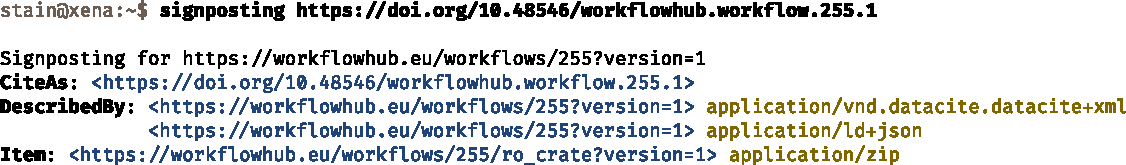
\includegraphics[width=\textwidth]{figures/ch04/signposting.pdf}
  \caption[FAIR Signposting]{~\textbf{FAIR Signposting}.
  FAIR Signposting on a workflow PID \cite{Bayarri 2022} 
  discovered from HTTP \texttt{Link:} headers using the
  Signposting tool\footnotemark{} shows
  machine-actionable navigation to content-negotiate for the metadata
  FDOs, as well as download bit sequence (FDOF3) as an RO-Crate zip.
  JSON-LD\footnotemark{} from
  workflowhub.eu follows the BioSchemas
  ComputationalWorkflow
  profile\footnotemark{}
  to give workflow details not included in DataCite's general 
  JSON-LD\footnotemark.
  }
  \label{fig:signposting}
\end{figure} 
% Evil goes here
\addtocounter{footnote}{-4}
\addtocounter{footnote}{1}\footnotetext{\url{https://pypi.org/project/signposting/}}
\addtocounter{footnote}{1}\footnotetext{\url{https://workflowhub.eu/workflows/255.jsonld}}
\addtocounter{footnote}{1}\footnotetext{\url{https://bioschemas.org/profiles/ComputationalWorkflow/1.0-RELEASE}}
\addtocounter{footnote}{1}\footnotetext{\url{https://data.crosscite.org/application/ld+json/10.48546/workflowhub.workflow.255.1}}
%%

Further work on RO-Crate profiles include to formalise links to the API
operations and repositories (FDOF5,FDOF7), to include PIDs of
profiles and types in the FAIR Signposting, and HTTP navigation to
individual resources within the RO-Crate.

RO-Crate has shown a broad adoption by communities across many
scientific disciplines, providing a lightweight, and therefore easy to
adopt, approach to generating FAIR Digital Objects. It is rapidly
becoming an integral part of the interoperability fabric between the
different components as demonstrated here for WorkflowHub, contributing
to building the European Open Science Cloud.

%\section{Packaging research artefacts with
RO-Crate}\label{packaging-research-artefacts-with-ro-crate}

An increasing number of researchers support reproducibility by including
pointers to and descriptions of datasets, software and methods in their
publications. However, scientific articles may be ambiguous, incomplete
and difficult to process by automated systems. In this paper we
introduce RO-Crate, an open, community-driven, and lightweight approach
to packaging research artefacts along with their metadata in a machine
readable manner. RO-Crate is based on Schema.org annotations in JSON-LD,
aiming to establish best practices to formally describe metadata in an
accessible and practical way for their use in a wide variety of
situations.

An RO-Crate is a structured archive of all the items that contributed to
a research outcome, including their identifiers, provenance, relations
and annotations. As a general purpose packaging approach for data and
their metadata, RO-Crate is used across multiple areas, including
bioinformatics, digital humanities and regulatory sciences. By applying
``just enough'' Linked Data standards, RO-Crate simplifies the process
of making research outputs FAIR while also enhancing research
reproducibility.

\subsection{Introduction}\label{introduction}

The move towards Open Science has increased the need and demand for the
publication of artefacts of the research process
\cite{Sefton 2021}. This is
particularly apparent in domains that rely on computational experiments;
for example, the publication of software, datasets and records of the
dependencies that such experiments rely on
\cite{Stodden 2016}.

It is often argued that the publication of these assets, and
specifically software
\cite{Lamprecht 2019}, workflows
\cite{ch5-55} and data, should
follow the FAIR principles
\cite{Wilkinson 2016}; namely, that
they are Findable, Accessible, Interoperable and Reusable. These
principles are agnostic to the \emph{implementation} strategy needed to
comply with them. Hence, there has been an increasing amount of work in
the development of platforms and specifications that aim to fulfil these
goals \cite{ch5-91}.

Important examples include data publication with rich metadata
(e.g.~Zenodo \cite{Dillen 2019}),
domain-specific data deposition (e.g.~PDB
\cite{Berman 2007}) and following
practices for reproducible research software
\cite{ch5-101} (e.g.~use
of containers). While these platforms are useful, experience has shown
that it is important to put greater emphasis on the interconnection of
the multiple artefacts that make up the research process
\cite{ch5-71}.

The notion of \textbf{Research Objects}
\cite{ch5-12}
(RO) was introduced to address this connectivity, providing semantically
rich \emph{aggregations} of (potentially distributed) resources with a
layer of structure over a research study; this is then to be delivered
in a \emph{machine-readable format}.

A Research Object combines the ability to bundle multiple types of
artefacts together, such as spreadsheets, code, examples, and figures.
The RO is augmented with annotations and relationships that describe the
artefacts' \emph{context} (e.g.~a CSV being used by a script, a figure
being a result of a workflow).

This notion of ROs provides a compelling vision as an approach for
implementing FAIR data. However, existing Research Object
implementations require a large technology stack
\cite{Belhajjame 2015}, are
typically tailored to a particular platform and are also not easily
usable by end-users.

To address this gap, a new community came together
\cite{Ó Carragáin 2019} to develop
\textbf{RO-Crate} --- an \emph{approach to package and aggregate
research artefacts with their metadata and relationships}. The aim of
this paper is to introduce RO-Crate and assess it as a strategy for
making multiple types of research artefacts FAIR. Specifically, the
contributions of this paper are as follows:

\begin{enumerate}
  \item[1.] An introduction to RO-Crate, its purpose and context;
  \item[2.] A guide to the RO-Crate community and tooling;
  \item[3.] Examples of RO-Crate usage, demonstrating its value as connective tissue for different artefacts from different communities.
\end{enumerate}

The rest of this paper is organised as follows. We first describe
RO-Crate through its development methodology that formed the RO-Crate
concept, showing its foundations in Linked Data and emerging principles.
We then define RO-Crate technically, before we introduce the community
and tooling. We move to analyse RO-Crate with respect to usage in a
diverse set of domains. Finally, we present related work and conclude
with some remarks including RO-Crate highlights and future work. The
appendix adds a formal definition of RO-Crate using First-Order logic.

\subsection{RO-Crate}\label{rocrate}

RO-Crate aims to provide an approach to packaging research artefacts
with their metadata that can be easily adopted. To illustrate this, let
us imagine a research paper reporting on the sequence analysis of
proteins obtained from an experiment on mice. The sequence output files,
sequence analysis code, resulting data and reports summarising
statistical measures are all important and inter-related research
artefacts, and consequently would ideally all be co-located in a
directory and accompanied with their corresponding metadata. In reality,
some of the artefacts (e.g.~data or software) will be recorded as
external reference to repositories that are not necessarily following
the FAIR principles. This conceptual directory, along with the
relationships between its constituent digital artefacts, is what the
RO-Crate model aims to represent, linking together all the elements of
an experiment that are required for the experiment's reproducibility and
reusability.

The question then arises as to how the directory with all this material
should be packaged in a manner that is accessible and usable by others.
This means programmatically and automatically accessible by machines and
human readable. A de facto approach to sharing collections of resources
is through compressed archives (e.g.~a zip file). This solves the
problem of ``packaging'', but it does not guarantee downstream access to
all artefacts in a programmatic fashion, nor describe the role of each
file in that particular research. Both features, the ability to
automatically access and reason about an object, are crucial and lead to
the need for explicit metadata about the contents of the folder,
describing each and linking them together.

Examples of metadata descriptions across a wide range of
domains\footnote{\url{https://rdamsc.bath.ac.uk/scheme-index}} abound within the
literature, both in research data management
\cite{Amorim 2016,ch5-46,ch5-75}
and within library and information
systems\footnote{\url{https://www.loc.gov/librarians/standards}} \cite{Mai Chan 1995,ch5-127}. However, many of these approaches require
knowledge of metadata schemas, particular annotation systems, or the
use of complex software stacks. Indeed, particularly within research,
these requirements have led to a lack of adoption and growing
frustration with current tooling and specifications
\cite{ch5-94,ch5-119,ch5-102}.

RO-Crate seeks to address this complexity by:

\begin{enumerate}
  \item[1.] being conceptually simple and easy to understand for developers;
  \item[2.] providing strong, easy tooling for integration into community projects;
  \item[3.] providing a strong and opinionated guide regarding current best practices;
  \item[4.] adopting de-facto standards that are widely used on the Web.
\end{enumerate}

In the following sections we demonstrate how the RO-Crate specification
and ecosystem achieve these goals.

\subsubsection{Development Methodology}\label{methodology}

It is a good question as to what base level we assume for `conceptually
simple'. We take simplicity to apply at two levels: for the
\emph{developers} who produce the platforms and for the \emph{data
practitioners} and users of those platforms.

For our development methodology we followed the mantra of working
closely with a small group to really get a deep understanding of
requirements and ensure rapid feedback loops. We created a pool of early
adopter projects from a range of disciplines and groups, primarily
addressing developers of platforms. Thus the base level for simplicity
was \textbf{developer friendliness}.

We assumed a developer familiar with making Web applications with JSON
data (who would then learn how to make \emph{RO-Crate JSON-LD}), which
informed core design choices for our JSON-level documentation approach
and RO-Crate serialization (section \vref{sec:implementation}). Our group of early
adopters, growing as the community evolved, drove the RO-Crate
requirements and provided feedback through our multiple communication
channels including bi-monthly meetings, which we describe in section \vref}sec:community} along with the established norms.

Addressing the simplicity of understanding and engaging with RO-Crate by
data practitioners is through the platforms, for example with
interactive tools (section \vref{sec:tooling}) like
Describo\footnote{\url{https://arkisto-platform.github.io/describo/}} \cite{ch5-78} and
Jupyter notebooks
\cite{ch5-70}, and by
close discussions with domain scientists on how to appropriately capture
what they determine to be relevant metadata. This ultimately requires a
new type of awareness and learning material separate from developer
specifications, focusing on the simplicity of extensibility to serve the
user needs, along with user-driven development of new RO-Crate Profiles
specific for their needs (section \vref{sec:inuse}).

\subsubsection{Conceptual Definition}\label{conceptual}

A key premise of RO-Crate is the existence of a wide variety of
resources on the Web that can help describe research. As such, RO-Crate
relies on the Linked Data principles
\cite{ch5-63}.
Figure \vref{fig:conceptual} shows the main conceptual
elements involved in an RO-Crate: The RO-Crate Metadata File (top)
describes the Research Object using structured metadata including
external references, coupled with the contained artefacts (bottom)
bundled and described by the RO-Crate.

The conceptual notion of a \emph{Research Object}
\cite{ch5-12}
is thus realised with the RO-Crate model and serialised using Linked
Data constructs within the RO-Crate metadata file.

\begin{figure}%[t!]
  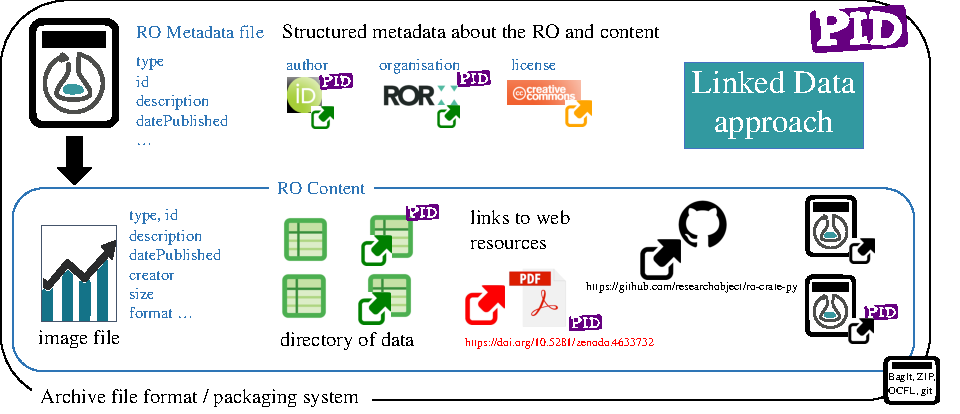
\includegraphics{content/images/ro-crate-overview.pdf}
  \caption{Conceptual overview of RO-Crate. A \emph{Persistent
  Identifier} (PID) \cite{ch5-86} points to a
  \emph{Research Object} (RO), which may be archived using different
  packaging approaches like BagIt \cite{ch5-74}, OCFL \cite
  {ch5-96}, git or ZIP. The RO is described within a \emph{RO-Crate
  Metadata File}, providing identifiers for \emph{authors} using ORCID,
  \emph{organisations} using Research Organization Registry (ROR) \cite
  {ch5-79} and licences such as Creative Commons using SPDX
  identifiers. The \emph{RO-Crate content} is further described with
  additional metadata following a Linked Data approach. Data can be
  embedded files and directories, as well as links to external Web
  resources, PIDs and nested RO-Crates.}
  \label{fig:conceptual}
\end{figure}

\subsubsubsection{Linked Data as a foundation}\label{linkeddata}

The \textbf{Linked Data} principles \cite{Bizer 2011}
(use of IRIs\footnote{\textbf{IRI}s \cite{rfc3987} are a generalisation
 of \textit{URI}s
(which include well-known http/https URLs), permitting international
Unicode characters without percent encoding, commonly used on the
browser address bar and in HTML5.} to identify resources (i.e. artefacts), resolvable via
HTTP, enriched with metadata and linked to each other) are core to
RO-Crate; therefore IRIs are used to identify an RO-Crate, its
constituent parts and metadata descriptions, and the properties and
classes used in the metadata.

RO-Crates are \emph{self-described} and follow the Linked Data
principles to describe all of their resources in both human and machine
readable manner. Hence, resources are identified using global
identifiers (absolute IRIs) where possible; and relationships between
two resources are defined with links.

The foundation of Linked Data and shared vocabularies also means that
multiple RO-Crates and other Linked Data resources can be indexed,
combined, queried, validated or transformed using existing Semantic Web
technologies such as SPARQL,\footnote{\url{https://www.w3.org/TR/sparql11-overview}}
SHACL\footnote{\url{https://www.w3.org/TR/shacl/}} and well established \textit{knowledge
graph} triple stores like Apache Jena\footnote{\url{https://jena.apache.org/}} and
OntoText GraphDB.\footnote{\url{https://www.ontotext.com/products/graphdb/}}

The possibilities of consuming\footnote{Some consideration is needed in processing of RO-Crates as
knowledge graphs, e.g. establishing absolute IRIs for files inside a
ZIP archive, detailed in the RO-Crate specification: \url
{https://www.researchobject.org/ro-crate/1.1/appendix/relative-uris.html}.} RO-Crate metadata with such
powerful tools gives another strong reason for using Linked Data as a
foundation. This use of mature Web\footnote{Note that an RO-Crate is not required to be published on the
Web, see Section~\ref{sec:selfdescribed}.} technologies also means its
developers and consumers are not restricted to the Research Object
aspects that have already been specified by the RO-Crate community, but
can extend and integrate RO-Crate in multiple standardised ways.


\subsubsubsection{RO-Crate is a self-described container}\label{selfdescribed}

An RO-Crate is defined\footnote{\url{https://www.researchobject.org/ro-crate/1.1/structure.html\#ro-crate-metadata-file-ro-crate-metadatajson}} as a self-described \textbf{Root Data Entity} that describes
and contains \emph{data entities}, which are further described by
referencing \emph{contextual entities}. A \textbf{data entity} is either
a \emph{file} (i.e.~a byte sequence stored on disk somewhere) or a
\emph{directory} (i.e.~set of named files and other directories). A file
does not need to be stored inside the RO-Crate root, it can be
referenced via a PID/IRI. A \textbf{contextual entity} exists outside
the information system (e.g.~a Person, a workflow language) and is
stored solely by its metadata. The representation of a \emph{data
entity} as a byte sequence makes it possible to store a variety of
research artefacts including not only data but also, for instance,
software and text.

The Root Data Entity is a directory, the \emph{RO-Crate Root},
identified by the presence of the \textbf{RO-Crate Metadata File}
\texttt{ro-crate-metadata.json} (top of Figure \vref{fig:conceptual}). This file describes the
RO-Crate using Linked Data, its content and related metadata using
Linked Data in JSON-LD format \cite{ch5-112}. This
is a W3C standard RDF serialisation that has become popular; it is easy
to read by humans while also offering some advantages for data exchange
on the Internet. JSON-LD, a subset of the widely supported and
well-known JSON format, has tooling available for many programming languages.\footnote{\url{https://json-ld.org/\#developers}}

The minimal requirements for the root data entity
metadata\footnote{\url{https://www.researchobject.org/ro-crate/1.1/root-data-entity.html\#direct-properties-of-the-root-data-entity}}
are \texttt{name}, \texttt{description} and \texttt{datePublished}, as well as a contextual
entity identifying its \texttt{license} -- additional metadata are commonly
added to entities depending on the purpose of the particular RO-Crate.

RO-Crates can be stored, transferred or published in multiple ways,
e.g.~BagIt \cite{ch5-74}, Oxford
Common File Layout \cite{ch5-96} (OCFL),
downloadable ZIP archives in Zenodo or through dedicated online
repositories, as well as published directly on the Web, e.g.~using
GitHub Pages.\footnote{\url{https://pages.github.com/}} Combined with Linked Data identifiers, this caters for a diverse set of storage and access
requirements across different scientific domains, from metagenomics
workflows producing hundreds of gigabytes of genome data to cultural
heritage records with access restrictions for personally identifiable
data. Specific \emph{RO-Crate profiles} (Section~\ref{sec:profiles}) may constrain serialization
and publication expectations, and require additional contextual types
and properties.

\subsubsubsection{Data Entities are described using Contextual
Entities}\label{contextualentities}

RO-Crate distinguishes between data and contextual
entities\footnote{\url{https://www.researchobject.org/ro-crate/1.1/contextual-entities.html\#contextual-vs-data-entities}} in a similar way to HTTP terminology's early
attempt to separate \emph{information} (data) and \emph{non-information}
(contextual) resources \cite{ch5-120}. Data entities are usually files and directories located by relative IRI
references within the RO-Crate Root, but they can also be Web resources
or restricted data identified with absolute IRIs, including
\emph{Persistent Identifiers} (PIDs)
\cite{ch5-86}.

As both types of entities are identified by IRIs, their distinction is
allowed to be blurry; data entities can be located anywhere and be
complex, while contextual entities can have a Web presence beyond their
description inside the RO-Crate. For instance
\texttt{https://orcid.org/0000-0002-1825-0097} is primarily an
identifier for a person, but secondarily it is also a Web page and a way
to refer to their academic work.

A particular IRI may appear as a contextual entity in one RO-Crate and
as a data entity in another; the distinction lies in the fact that data
entities can be considered to be \emph{contained} or captured by that
RO-Crate (\textit{RO Content} in Fig.~\ref{fig:conceptual}), while contextual entities mainly \emph{explain} an RO-Crate or its
content (although this distinction is not a formal requirement).

In RO-Crate, a referenced contextual entity (e.g.~a person identified by
ORCID) should always be described within the RO-Crate Metadata File with
at least a \emph{type} and \emph{name}, even where their PID might
resolve to further Linked Data. This is so that clients are not required
to follow every link for presentation purposes, for instance HTML
rendering. Similarly any imported extension
terms\footnote{\url{https://www.researchobject.org/ro-crate/1.1/appendix/jsonld.html\#extending-ro-crate}} would themselves also have a human-readable description in the
case where their PID does not directly resolve to human-readable
documentation.

Figure \vref{fig:uml} shows a simplified UML class
diagram of RO-Crate, highlighting the different types of data entities
and contextual entities that can be aggregated and related. While an
RO-Crate would usually contain one or more data entities
(\texttt{hasPart}), it may also be a pure aggregation of contextual
entities (\texttt{mentions}).

\begin{figure}%[t!]
  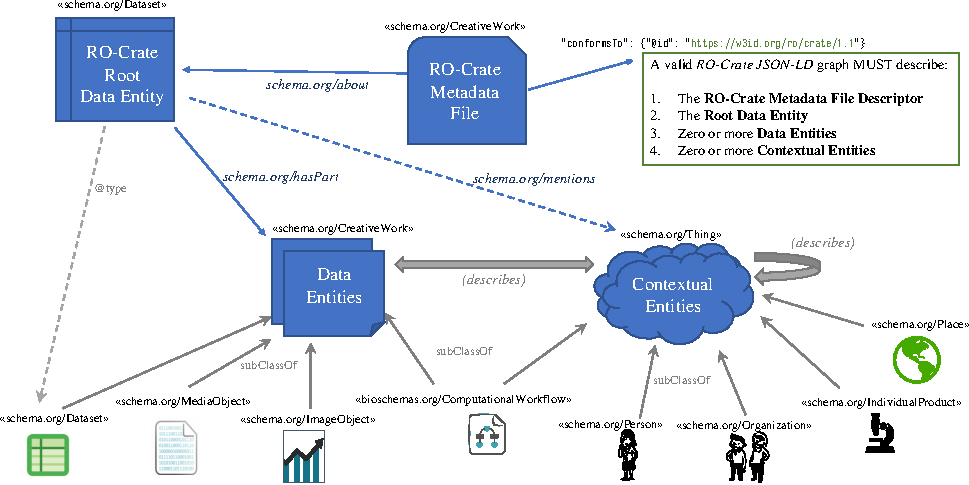
\includegraphics[width=0.9\textwidth]{content/images/ro-crate-uml.pdf}
  \caption{Simplified UML class diagram of RO-Crate. The \emph
  {RO-Crate Metadata File} conforms to a version of the specification;
  and contains a JSON-LD graph \cite{ch5-112} that describes the
  entities that make up the RO-Crate. The \emph{RO-Crate Root Data
  Entity} represent the Research Object as a dataset. The RO-Crate
  aggregates \emph{data entities} (\texttt{hasPart}) which are further
  described using \emph{contextual entities} (which may include
  aggregated and non-aggregated data entities). Multiple types and
  relations from Schema.org allow annotations to be more specific,
  including figures, nested datasets, computational workflows, people,
  organisations, instruments and places. Contextual entities not
  otherwise cross-referenced from other entities' properties (\emph
  {describes}) can be grouped under the root entity (\texttt{mentions}).}
  \label{fig:uml}
\end{figure}

%%% SYNCED 


\subsubsubsection{Guide through Recommended
Practices}\label{recommendedpractices}

RO-Crate as a specification aims to build a set of recommended practices
on how to practically apply existing standards in a common way to
describe research outputs and their provenance, without having to learn
each of the underlying technologies in detail.

As such, the \href{https://w3id.org/ro/crate/1.1}{RO-Crate 1.1}
specification \cite{ch5-106}
can be seen as an opinionated and example-driven guide to writing
\href{https://schema.org/}{Schema.org}
\cite{ch5-62} metadata as
JSON-LD
\href{https://www.w3.org/TR/2014/REC-json-ld-20140116/}{{[}112{]}} (see
section on \protect\hyperlink{implementation}{implementation}, which
leaves it open for implementers to include additional metadata using
other Schema.org types and properties, or even additional Linked Data
vocabularies/ontologies or their own ad-hoc terms.

However the primary purpose of the RO-Crate specification is to assist
developers in leveraging Linked Data principles for the focused purpose
of describing Research Objects in a structured language, while reducing
the steep learning curve otherwise associated with Semantic Web
adaptation, like development of ontologies, identifiers, namespaces, and
RDF serialization choices.

\subsubsection{Ensuring Simplicity}\label{simplicity}

One aim of RO-Crate is to be conceptually simple. This simplicity has
been repeatedly checked and confirmed through an informal community
review process. For instance, in the discussion on supporting
\href{https://github.com/ResearchObject/ro-crate/issues/71}{ad-hoc
vocabularies} in RO-Crate, the community explored potential Linked Data
solutions. The conventional wisdom in
\href{https://www.w3.org/TR/swbp-vocab-pub/}{RDF best practices} is to
establish a vocabulary with a new IRI namespace, formalised using
\href{http://www.w3.org/TR/2014/REC-rdf-schema-20140225/}{RDF Schema} or
\href{http://www.w3.org/TR/2012/REC-owl2-overview-20121211/}{OWL}
ontologies. However, this may seem an excessive learning curve for
non-experts in semantic knowledge representation, and the RO-Crate
community instead agreed on a dual lightweight approach: (i)
\href{https://www.researchobject.org/ro-crate/1.1/appendix/jsonld.html\#adding-new-or-ad-hoc-vocabulary-terms}{Document}
how projects with their own Web-presence can make a pure HTML-based
vocabulary, and (ii) provide a community-wide PID namespace under
\texttt{https://w3id.org/ro/terms} that redirect to simple CSV files
\href{https://github.com/ResearchObject/ro-terms}{maintained in GitHub}.

To further verify this idea of simplicity, we have formalised the
RO-Crate definition (see Appendix on
\protect\hyperlink{formaldefinition}{Formal Definition}). An important
result of this exercise is that the underlying data structure of
RO-Crate, although conceptually a graph, is represented as a
depth-limited tree. This formalisation also emphasises the
\emph{boundedness} of the structure; namely, the fact that elements are
specifically identified as being either semantically \emph{contained} by
the RO-Crate as \emph{Data Entities} (\texttt{hasPart}) or mainly
referenced (\texttt{mentions}) and typed as \emph{external} to the
Research Object as \emph{Contextual Entities}. It is worth pointing out
that this semantic containment can extend beyond the physical
containment of files residing within the RO-Crate Root directory on a
given storage system, as the RO-Crate data entities may include any data
resource globally identifiable using IRIs.

\subsubsection{Extensibility and RO-Crate profiles}\label{profiles}

The RO-Crate specification provides a core set of conventions to
describe research outputs using types and properties applicable across
scientific domains. However we have found that domain-specific use of
RO-Crate will, implicitly or explicitly, form a specialised
\textbf{profile} of RO-Crate; i.e., \emph{a set of conventions, types
and properties that are minimally required and one can expect to be
present in that subset of RO-Crates}. For instance, RO-Crates used for
exchange of workflows will have to contain a data entity of type
\texttt{ComputationalWorkflow}, or cultural heritage records should have
a \texttt{contentLocation}.

Making such profiles explicit allow further reliable programmatic
consumption and generation of RO-Crates beyond the core types defined in
the RO-Crate specification. Following the RO-Crate mantra of
\emph{guidance over strictness}, profiles are mainly \emph{duck-typing}
rather than strict syntactic or semantic types, but may also have
corresponding machine-readable schemas at multiple levels (file formats,
JSON, RDF shapes, RDFS/OWL semantics).

The next version of the RO-Crate specification 1.2 will define a
\href{https://www.researchobject.org/ro-crate/1.2-DRAFT/profiles}{formalization}
for publishing and declaring conformance to RO-Crate profiles. Such a
profile is primarily a human-readable document of before-mentioned
expectations and conventions, but may also define a machine-readable
profile as a \textbf{Profile Crate}: Another RO-Crate that describe the
profile and in addition can list schemas for validation, compatible
software, applicable repositories, serialization/packaging formats,
extension vocabularies, custom JSON-LD contexts and examples (see for
example the
\href{https://w3id.org/workflowhub/workflow-ro-crate/}{Workflow RO-Crate
profile}).

In addition, there are sometimes existing domain-specific metadata
formats, but they are either not RDF-based (and thus time-consuming to
construct terms for in JSON-LD) or are at a different granularity level
that might become overwhelming if represented directly in the RO-Crate
Metadata file (e.g.~W3C PROV bundle detailing every step execution of a
workflow run
\cite{ch5-68}). RO-Crate
allows such \emph{alternative metadata files} to co-exist, and be
described as data entities with references to the standards and
vocabularies they conform to. This simplifies further programmatic
consumption even where no filename or file extension conventions have
emerged for those metadata formats.

Section on \protect\hyperlink{inuse}{in use} examines the observed
specializations of RO-Crate use in several domains and their emerging
profiles.

\subsubsection{Technical implementation of the RO-Crate
model}\label{implementation}

The RO-Crate conceptual model has been realised using JSON-LD and
Schema.org in a prescriptive form as discussed in section on
\protect\hyperlink{conceptual}{conceptual definition}. These technical
choices were made to cater for simplicity from a developer perspective
(as introduced in section on
\protect\hyperlink{methodology}{methodology}).

\href{https://json-ld.org/}{JSON-LD}
\href{https://www.w3.org/TR/2014/REC-json-ld-20140116/}{{[}112{]}}
provides a way to express Linked Data as a JSON structure, where a
\emph{context} provides mapping to RDF properties and classes. While
JSON-LD cannot map arbitrary JSON structures to RDF, we found that it
does lower the barrier compared to other RDF syntaxes, as the JSON
syntax nowadays is a common and popular format for data exchange on the
Web.

However, JSON-LD alone has too many degrees of freedom and hidden
complexities for software developers to reliably produce and consume
without specialised expertise or large RDF software frameworks. A large
part of the RO-Crate specification is therefore dedicated to describing
the acceptable subset of JSON structures.

\subsubsubsection{RO-Crate JSON-LD}\label{jsonld}

RO-Crate
\href{https://www.researchobject.org/ro-crate/1.1/appendix/jsonld.html}{mandates}
the use of flattened, compacted JSON-LD in the RO-Crate Metadata file
\texttt{ro-crate-metadata.json}\footnote{The avid reader may spot that
  the RO-Crate Metadata file use the extension \texttt{.json} instead of
  \texttt{.jsonld}, this is to emphasise the developer expectations as a
  JSON format, while the file's JSON-LD nature is secondary. See
  \href{https://github.com/ResearchObject/ro-crate/issues/82}{ResearchObject/ro-crate\#82}.}
where a single \texttt{@graph} array contains all the data and
contextual entities in a flat list. An example can be seen in the
JSON-LD snippet in Listing 1 below, describing a simple RO-Crate
containing data entities described using contextual entities:

\begin{Shaded}
\begin{Highlighting}[]
\FunctionTok{\{} \DataTypeTok{"@context"}\FunctionTok{:} \StringTok{"https://w3id.org/ro/crate/1.1/context"}\FunctionTok{,}
  \DataTypeTok{"@graph"}\FunctionTok{:} \OtherTok{[}
      \FunctionTok{\{} \DataTypeTok{"@id"}\FunctionTok{:} \StringTok{"ro{-}crate{-}metadata.json"}\FunctionTok{,}      
        \DataTypeTok{"@type"}\FunctionTok{:} \StringTok{"CreativeWork"}\FunctionTok{,}
        \DataTypeTok{"conformsTo"}\FunctionTok{:} \FunctionTok{\{}\DataTypeTok{"@id"}\FunctionTok{:} \StringTok{"https://w3id.org/ro/crate/1.1"}\FunctionTok{\},}
        \DataTypeTok{"about"}\FunctionTok{:} \FunctionTok{\{}\DataTypeTok{"@id"}\FunctionTok{:} \StringTok{"./"}\FunctionTok{\}}
      \FunctionTok{\}}\OtherTok{,}
      \FunctionTok{\{} \DataTypeTok{"@id"}\FunctionTok{:} \StringTok{"./"}\FunctionTok{,}
        \DataTypeTok{"@type"}\FunctionTok{:} \StringTok{"Dataset"}\FunctionTok{,}
        \DataTypeTok{"name"}\FunctionTok{:} \StringTok{"A simplified RO{-}Crate"}\FunctionTok{,}
        \DataTypeTok{"author"}\FunctionTok{:} \FunctionTok{\{}\DataTypeTok{"@id"}\FunctionTok{:} \StringTok{"\#alice"}\FunctionTok{\},}
        \DataTypeTok{"license"}\FunctionTok{:} \FunctionTok{\{}\DataTypeTok{"@id"}\FunctionTok{:} \StringTok{"https://spdx.org/licenses/CC{-}BY{-}4.0"}\FunctionTok{\},}
        \DataTypeTok{"datePublished"}\FunctionTok{:} \StringTok{"2021{-}11{-}02T16:04:43Z"}\FunctionTok{,}
        \DataTypeTok{"hasPart"}\FunctionTok{:} \OtherTok{[}
          \FunctionTok{\{}\DataTypeTok{"@id"}\FunctionTok{:} \StringTok{"survey{-}responses{-}2019.csv"}\FunctionTok{\}}\OtherTok{,}
          \FunctionTok{\{}\DataTypeTok{"@id"}\FunctionTok{:} \StringTok{"https://example.com/pics/5707039334816454031\_o.jpg"}\FunctionTok{\}}
        \OtherTok{]}
      \FunctionTok{\}}\OtherTok{,}
      \FunctionTok{\{} \DataTypeTok{"@id"}\FunctionTok{:} \StringTok{"survey{-}responses{-}2019.csv"}\FunctionTok{,}
        \DataTypeTok{"@type"}\FunctionTok{:} \StringTok{"File"}\FunctionTok{,}
        \DataTypeTok{"about"}\FunctionTok{:} \FunctionTok{\{}\DataTypeTok{"@id"}\FunctionTok{:} \StringTok{"https://example.com/pics/5707039334816454031\_o.jpg"}\FunctionTok{\},}
        \DataTypeTok{"author"}\FunctionTok{:} \FunctionTok{\{}\DataTypeTok{"@id"}\FunctionTok{:} \StringTok{"\#alice"}\FunctionTok{\}}
      \FunctionTok{\}}\OtherTok{,}
      \FunctionTok{\{} \DataTypeTok{"@id"}\FunctionTok{:} \StringTok{"https://example.com/pics/5707039334816454031\_o.jpg"}\FunctionTok{,}
        \DataTypeTok{"@type"}\FunctionTok{:} \OtherTok{[}\StringTok{"File"}\OtherTok{,} \StringTok{"ImageObject"}\OtherTok{]}\FunctionTok{,}
        \DataTypeTok{"contentLocation"}\FunctionTok{:} \FunctionTok{\{}\DataTypeTok{"@id"}\FunctionTok{:} \StringTok{"http://sws.geonames.org/8152662/"}\FunctionTok{\},}
        \DataTypeTok{"author"}\FunctionTok{:} \FunctionTok{\{}\DataTypeTok{"@id"}\FunctionTok{:} \StringTok{"https://orcid.org/0000{-}0002{-}1825{-}0097"}\FunctionTok{\}}
      \FunctionTok{\}}\OtherTok{,}
      \FunctionTok{\{} \DataTypeTok{"@id"}\FunctionTok{:} \StringTok{"\#alice"}\FunctionTok{,}
        \DataTypeTok{"@type"}\FunctionTok{:} \StringTok{"Person"}\FunctionTok{,}
        \DataTypeTok{"name"}\FunctionTok{:} \StringTok{"Alice"}
      \FunctionTok{\}}\OtherTok{,}
      \FunctionTok{\{} \DataTypeTok{"@id"}\FunctionTok{:} \StringTok{"https://orcid.org/0000{-}0002{-}1825{-}0097"}\FunctionTok{,}
        \DataTypeTok{"@type"}\FunctionTok{:} \StringTok{"Person"}\FunctionTok{,}
        \DataTypeTok{"name"}\FunctionTok{:} \StringTok{"Josiah Carberry"}
      \FunctionTok{\}}\OtherTok{,}
      \FunctionTok{\{} \DataTypeTok{"@id"}\FunctionTok{:} \StringTok{"http://sws.geonames.org/8152662/"}\FunctionTok{,}
        \DataTypeTok{"@type"}\FunctionTok{:} \StringTok{"Place"}\FunctionTok{,}
        \DataTypeTok{"name"}\FunctionTok{:} \StringTok{"Catalina Park"}
      \FunctionTok{\}}\OtherTok{,}
      \FunctionTok{\{} \DataTypeTok{"@id"}\FunctionTok{:} \StringTok{"https://spdx.org/licenses/CC{-}BY{-}4.0"}\FunctionTok{,}
        \DataTypeTok{"@type"}\FunctionTok{:} \StringTok{"CreativeWork"}\FunctionTok{,}
        \DataTypeTok{"name"}\FunctionTok{:} \StringTok{"Creative Commons Attribution 4.0"}
      \FunctionTok{\}}
  \OtherTok{]}
\FunctionTok{\}}
\end{Highlighting}
\end{Shaded}

\textbf{Listing 1}: Simplified\footnote{Recommended properties for types
  shown in Listing 1 also include \texttt{affiliation},
  \texttt{citation}, \texttt{contactPoint}, \texttt{description},
  \texttt{encodingFormat}, \texttt{funder}, \texttt{geo},
  \texttt{identifier}, \texttt{keywords}, \texttt{publisher}; these
  properties and corresponding contextual entities are excluded here for
  brevity. See
  \href{https://www.researchobject.org/2021-packaging-research-artefacts-with-ro-crate/listing1/}{complete
  example}.} RO-Crate metadata file showing the flattened compacted
JSON-LD \texttt{@graph} array containing the data entities and
contextual entities, cross-referenced using \texttt{@id}. The
\texttt{ro-crate-metadata.json} entity self-declares conformance with
the RO-Crate specification using a versioned persistent identifier,
further RO-Crate descriptions are on the root data entity \texttt{./} or
any of the referenced data or contextual entities. This is exemplified
by the data entity \texttt{ImageObject} referencing contextual entities
for \texttt{contentLocation} and \texttt{author} that differs from that
of the overall RO-Crate. In this crate, \texttt{about} of the CSV data
entity reference the \texttt{ImageObject}, which then take the roles of
both a data entity and contextual entity. While \texttt{Person} entities
ideally are identified with ORCID PIDs as for Josiah, \texttt{\#alice}
is here in contrast an RO-Crate local identifier, highlighting the
pragmatic ``just enough'' Linked Data approach. \normalsize

In this flattened profile of JSON-LD, each \texttt{\{entity\}} are
directly under \texttt{@graph} and represents the RDF triples with a
common \emph{subject} (\texttt{@id}), mapped \emph{properties} like
\texttt{hasPart}, and \emph{objects} --- as either literal
\texttt{"string"} values, referenced \texttt{\{objects\}} (which
properties are listed in its own entity), or a JSON \texttt{{[}list{]}}
of these. If processed as JSON-LD, this forms an RDF graph by matching
the \texttt{@id} IRIs and applying the \texttt{@context} mapping to
Schema.org terms. \normalsize

\hypertarget{flattened-json-ld}{%
\paragraph{Flattened JSON-LD}\label{flattened-json-ld}}

When JSON-LD 1.0
\href{https://www.w3.org/TR/2014/REC-json-ld-20140116/}{{[}112{]}} was
proposed, one of the motivations was to seamlessly apply an RDF nature
on top of regular JSON as frequently used by Web APIs. JSON objects in
APIs are frequently nested with objects at multiple levels, and the
perhaps most common form of JSON-LD is the
\href{https://json-ld.org/spec/REC/json-ld/20140116/\#compacted-document-form}{compacted
form} which follows this expectation
(\href{https://www.w3.org/TR/2020/REC-json-ld11-20200716/}{JSON-LD 1.1}
further expands these capabilities, e.g.~allowing nested
\texttt{@context} definitions).

While this feature of JSON-LD can be seen as a way to ``hide'' its RDF
nature, we found that the use of nested trees (e.g.~a \texttt{Person}
entity appearing as \texttt{author} of a \texttt{File} which nests under
a \texttt{Dataset} with \texttt{hasPart}) counter-intuitively forces
consumers to consider the JSON-LD as an RDF Graph, since an identified
\texttt{Person} entity can appear at multiple and repeated points of the
tree (e.g.~author of multiple files), necessitating node merging or
duplication, which can become complicated as this approach also invites
the use of \emph{blank nodes} (entities missing \texttt{@id}).

By comparison, a single flat \texttt{@graph} array approach, as required
by RO-Crate, means that applications can choose to process and edit each
entity as pure JSON by a simple lookup based on \texttt{@id}. At the
same time, lifting all entities to the same level reflects the Research
Object principles
\cite{ch5-12}
in that describing the context and provenance is just as important as
describing the data, and the requirement of \texttt{@id} of every entity
forces RO-Crate generators to consciously
\href{https://www.researchobject.org/ro-crate/1.1/appendix/jsonld.html\#describing-entities-in-json-ld}{consider
existing IRIs and identifiers}.

\hypertarget{json-ld-context}{%
\paragraph{JSON-LD context}\label{json-ld-context}}

In JSON-LD, the \texttt{@context} is a reference to another JSON-LD
document that provides mapping from JSON keys to Linked Data term IRIs,
and can enable various JSON-LD directives to cater for customised JSON
structures for translating to RDF.

RO-Crate reuses vocabulary terms and IRIs from Schema.org, but provides
its own versioned \href{https://w3id.org/ro/crate/1.1/context}{JSON-LD
context}, which has a flat list with the mapping from JSON-LD keys to
their IRI equivalents (e.g.~key \texttt{"author"} maps to the
\url{http://schema.org/author} property).

The rationale behind this decision is to support JSON-based RO-Crate
applications that are largely unaware of JSON-LD, that still may want to
process the \texttt{@context} to find or add Linked Data definitions of
otherwise unknown properties and types. Not reusing the official
Schema.org context means RO-Crate is also able to map in additional
vocabularies where needed, namely the \emph{Portland Common Data Model}
(PCDM) \href{https://github.com/duraspace/pcdm/wiki}{{[}Cossu 2018{]}} for
repositories and Bioschemas
\href{https://iswc2017.semanticweb.org/paper-579/}{{[}58{]}} for
describing computational workflows. RO-Crate profiles may
\href{https://www.researchobject.org/ro-crate/1.1/appendix/jsonld.html\#extending-ro-crate}{extend}
the \texttt{@context} to re-use additional domain-specific ontologies.

Similarly, while the Schema.org context
\href{https://schema.org/version/13.0/schemaorg-current-http.jsonld}{currently}
have \texttt{"@type":\ "@id"} annotations for implicit object
properties, RO-Crate JSON-LD distinguishes explicitly between references
to other entities (\texttt{\{"@id":\ "\#alice"\}}) and string values
(\texttt{"Alice"}) --- meaning RO-Crate applications can find references
for corresponding entities and IRIs without parsing the
\texttt{@context} to understand a particular property. Notably this is
exploited by the \emph{ro-crate-html-js}
\href{https://www.npmjs.com/package/ro-crate-html-js}{{[}95{]}} tool to
provide reliable HTML rendering for otherwise unknown properties and
types.

\hypertarget{community}{%
\subsubsection{RO-Crate Community}\label{community}}

The RO-Crate conceptual model, implementation and best practices are
developed by a growing community of researchers, developers and
publishers. RO-Crate's community is a key aspect of its effectiveness in
making research artefacts FAIR. Fundamentally, the community provides
the overall context of the implementation and model and ensures its
interoperability.

The RO-Crate community consists of:

\begin{enumerate}
\def\labelenumi{\arabic{enumi}.}
\tightlist
\item
  a diverse set of people representing a variety of stakeholders;
\item
  a set of collective norms;
\item
  an open platform that facilitates communication (GitHub, Google Docs,
  monthly teleconferences).
\end{enumerate}

\hypertarget{people}{%
\paragraph{People}\label{people}}

The initial concept of RO-Crate was formed at the first Workshop on
Research Objects
(\href{https://www.researchobject.org/ro2018/}{RO2018}), held as part of
the IEEE conference on eScience. This workshop followed up on
considerations made at a
\href{https://rd-alliance.org/approaches-research-data-packaging-rda-11th-plenary-bof-meeting}{Research
Data Alliance (RDA) meeting on Research Data Packaging} that found
similar goals across multiple data packaging efforts
\cite{Ó Carragáin 2019}: simplicity,
structured metadata and the use of JSON-LD.

An important outcome of discussions that took place at RO2018 was the
conclusion that the original Wf4Ever Research Object ontologies
\cite{Belhajjame 2015}, in
principle sufficient for packaging research artefacts with rich
descriptions, were, in practice, considered inaccessible for regular
programmers (e.g., Web developers) and in danger of being
incomprehensible for domain scientists due to their reliance on Semantic
Web technologies and other ontologies.

DataCrate \cite{ch5-103} was
presented at RO2018 as a promising lightweight alternative approach, and
an agreement was made by a group of volunteers to attempt building what
was initially called \emph{``RO Lite''} as a combination of DataCrate's
implementation and Research Object's principles.

This group, originally made up of library and Semantic Web experts, has
subsequently grown to include domain scientists, developers, publishers
and more. This perspective of multiple views led to the specification
being used in a variety of domains, from bioinformatics and regulatory
submissions to humanities and cultural heritage preservation.

The RO-Crate community is strongly engaged with the European-wide
biology/bioinformatics collaborative e-Infrastructure ELIXIR
\cite{Crosswell 2012}, along
with \href{https://eosc.eu/}{European Open Science Cloud} (EOSC)
projects including \href{https://www.eosc-life.eu/}{EOSC-Life},
\href{https://fairplus-project.eu/}{FAIRplus},
\href{https://cs3mesh4eosc.eu/}{CS3MESH4EOSC} and
\href{https://by-covid.eu/}{BY-COVID}. RO-Crate has also established
collaborations with Bioschemas
\href{https://iswc2017.semanticweb.org/paper-579/}{{[}58{]}}, GA4GH
\cite{ch5-99}, OpenAIRE
\href{https://doi.org/10.5860/crln.76.6.9326}{{[}100{]}} and multiple
H2020 projects.

A key set of stakeholders are developers: the RO-Crate community has
made a point of attracting developers who can implement the
specifications but, importantly, keeps ``developer user experience'' in
mind. This means that the specifications are straightforward to
implement and thus do not require expertise in technologies that are not
widely deployed.

This notion of catering to ``developer user experience'' is an example
of the set of norms that have developed and now define the community.

\hypertarget{norms}{%
\paragraph{Norms}\label{norms}}

The RO-Crate community is driven by informal conventions and notions
that are prevalent but not neccessarily written down. Here, we distil
what we as authors believe are the critical set of norms that have
facilitated the development of RO-Crate and contributed to the ability
for RO-Crate research packages to be FAIR. This is not to say that there
are no other norms within the community nor that everyone in the
community holds these uniformly. Instead, what we emphasise is that
these norms are helpful and also shaped by community practices.

\begin{enumerate}
\def\labelenumi{\arabic{enumi}.}
\tightlist
\item
  Simplicity
\item
  Developer friendliness
\item
  Focus on examples and best practices rather than rigorous
  specification
\item
  Reuse ``just enough'' Web standards
\end{enumerate}

A core norm of RO-Crate is that of \textbf{simplicity}, which sets the
scene for how we guide developers to structure metadata with RO-Crate.
We focus mainly on documenting simple approaches to the most common use
cases, such as authors having an affiliation. This norm also influences
our take on \textbf{developer friendliness}; for instance, we are using
the Web-native JSON format, allowing only a few of JSON-LD's flexible
Linked Data features. Moreover, the RO-Crate documentation is largely
built up by \textbf{examples} showcasing \textbf{best practices}, rather
than rigorous specifications. We build on existing \textbf{Web
standards} that themselves are defined rigorously, which we utilise
\emph{``\textbf{just enough}''} in order to benefit from the advantages
of Linked Data (e.g., extensions by namespaced vocabularies), without
imposing too many developer choices or uncertainties (e.g., having to
choose between the many RDF syntaxes).

While the above norms alone could easily lead to the creation of ``yet
another'' JSON format, we keep the goal of \textbf{FAIR
interoperability} of the captured metadata, and therefore follow closely
FAIR best practices and current developments such as data citations,
PIDs, open repositories and recommendations for sharing research outputs
and software.

\hypertarget{open-platforms}{%
\paragraph{Open Platforms}\label{open-platforms}}

The critical infrastructure that enables the community around RO-Crate
is the use of open development platforms. This underpins the importance
of open community access to supporting FAIR. Specifically, it is
difficult to build and consume FAIR research artefacts without being
able to access the specifications, understand how they are developed,
know about any potential implementation issues, and discuss usage to
evolve best practices.

The development of RO-Crate was driven by capturing documentation of
real-life examples and best practices rather than creating a rigorous
specification. At the same time, we agreed to be opinionated on the
syntactic form to reduce the jungle of implementation choices; we wanted
to keep the important aspects of Linked Data to adhere to the FAIR
principles while retaining the option of combining and extending the
structured metadata using the existing Semantic Web stack, not just
build a standalone JSON format.

Further work during 2019 started adapting the DataCrate documentation
through a more collaborative and exploratory \emph{RO Lite} phase,
initially using Google Docs for review and discussion, then moving to
GitHub as a collaboration space for developing what is now the RO-Crate
specification,
\href{https://github.com/researchobject/ro-crate/}{maintained} as
Markdown in GitHub Pages and published through Zenodo.

In addition to the typical Open Source-style development with GitHub
issues and pull requests, the RO-Crate Community have, at time of
writing, two regular monthly calls, a Slack channel and a mailing list
for coordinating the project; also many of its participants collaborate
on RO-Crate at multiple conferences and coding events such as the
\href{https://biohackathon-europe.org/}{ELIXIR BioHackathon}. The
community is jointly developing the RO-Crate specification and Open
Source tools, as well as providing support and considering new use
cases. The
\href{https://www.researchobject.org/ro-crate/community}{RO-Crate
Community} is open for anyone to join, to equally participate under a
code of conduct, and as of October 2021 has more than 50 members (see
Appendix \protect\hyperlink{communitylist}{RO-Crate Community}).

\hypertarget{tooling}{%
\subsection{RO-Crate Tooling}\label{tooling}}

The work of the community has led to the development of a number of
tools for creating and using RO-Crates. Table 1 shows the current set of
implementations. Reviewing this list, one can see support for commonly
used programming languages, including Python, JavaScript, and Ruby.
Additionally, the tools can be integrated into commonly used research
environments, in particular, the command line tool
\emph{ro-crate-html-js}
\href{https://www.npmjs.com/package/ro-crate-html-js}{{[}95{]}} for
creating a human-readable preview of an RO-Crate as a sidecar HTML file.
Furthermore, there are tools that cater to end-users (\emph{Describo}
\href{https://arkisto-platform.github.io/describo/}{{[}78{]}},
\emph{WorkflowHub} \href{https://w3id.org/workflowhub/}{{[}124{]}}), in
order to simplify creating and managing RO-Crate. For example, Describo
was developed to help researchers of the Australian
\href{https://criminalcharacters.com/}{Criminal Characters project} to
annotate historical prisoner records for greater insight into the
history of Australia
\cite{ch5-97}.

While the development of these tools is promising, our analysis of their
maturity status shows that the majority of them are in the Beta stage.
This is partly due to the fact that the RO-Crate specification itself
only recently reached 1.0 status, in November 2019
\cite{ch5-105}. Now that there
is a fixed point of reference: With version 1.1 (October 2020)
\cite{ch5-107} RO-Crate has
stabilised based on feedback from application development, and now we
are seeing a further increase in the maturity of these tools, along with
the creation of new ones.

Given the stage of the specification, these tools have been primarily
targeting developers, essentially providing them with the core libraries
for working with RO-Crate. Another target has been that of research data
managers who need to manage and curate large amounts of data.

\begin{longtable}[]{@{}
  >{\raggedright\arraybackslash}p{(\columnwidth - 8\tabcolsep) * \real{0.15}}
  >{\raggedright\arraybackslash}p{(\columnwidth - 8\tabcolsep) * \real{0.11}}
  >{\raggedright\arraybackslash}p{(\columnwidth - 8\tabcolsep) * \real{0.34}}
  >{\raggedright\arraybackslash}p{(\columnwidth - 8\tabcolsep) * \real{0.09}}
  >{\raggedright\arraybackslash}p{(\columnwidth - 8\tabcolsep) * \real{0.30}}@{}}
\toprule
Tool Name & Targets & Language /Platform & Status & Brief Description \\
\midrule
\endhead
Describo \href{https://arkisto-platform.github.io/describo/}{{[}78{]}} &
Research Data Managers & NodeJS (Desktop) & RC & Interactive desktop
application to create, update and export RO-Crates for different
profiles \\
Describo Online
\href{https://arkisto-platform.github.io/describo-online/}{{[}77{]}} &
Platform developers & NodeJS (Web) & Alpha & Web-based application to
create RO-Crates using cloud storage \\
ro-crate-excel
\href{https://www.npmjs.com/package/ro-crate-excel}{{[}84{]}} & Data
managers & JavaScript & Beta & Command-line tool to create/edit
RO-Crates with spreadsheets \\
ro-crate-html-js
\href{https://www.npmjs.com/package/ro-crate-html-js}{{[}95{]}} &
Developers & JavaScript & Beta & HTML rendering of RO-Crate \\
ro-crate-js
\href{https://github.com/UTS-eResearch/ro-crate-js}{{[}49{]}} & Research
Data Managers & JavaScript & Alpha & Library for creating/manipulating
crates; basic validation code \\
ro-crate-ruby
\href{https://github.com/ResearchObject/ro-crate-ruby}{{[}Bacall 2022b{]}} &
Developers & Ruby & Beta & Ruby library for reading/writing RO-Crate,
with workflow support \\
ro-crate-py \href{https://doi.org/10.5281/zenodo.3956493}{{[}Droesbeke 2022{]}}) &
Developers & Python & Alpha & Object-oriented Python library for
reading/writing RO-Crate and use by Jupyter Notebook \\
WorkflowHub \href{https://w3id.org/workflowhub/}{{[}124{]}} & Workflow
users & Ruby & Beta & Workflow repository; imports and exports Workflow
RO-Crate \\
Life Monitor \href{https://about.lifemonitor.eu/}{{[}CRS4 2022{]}} & Workflow
developers & Python & Alpha & Workflow testing and monitoring service;
Workflow Testing profile of RO-Crate \\
SCHeMa \href{https://arxiv.org/abs/2103.13138v1}{{[}118{]}} & Workflow
users & PHP & Alpha & Workflow execution using RO-Crate as exchange
mechanism
\cite{10.5281/zenodo.4671709} \\
galaxy2cwl \href{https://github.com/workflowhub-eu/galaxy2cwl}{{[}50{]}}
& Workflow developers & Python & Alpha & Wraps Galaxy workflow as
Workflow RO-Crate \\
Modern PARADISEC \href{https://github.com/CoEDL/modpdsc/}{{[}51{]}} &
Repository managers & Platform & Beta & Cultural Heritage portal based
on OCFL and RO-Crate \\
ONI express
\href{https://arkisto-platform.github.io/tools/portal/}{{[}115{]}} &
Repository managers & Platform & Beta & Platform for publishing data and
documents stored in an OCFL repository via a Web interface \\
ocfl-tools \href{https://github.com/CoEDL/ocfl-tools}{{[}52{]}} &
Developers & JavaScript (CLI) & Beta & Tools for managing RO-Crates in
an OCFL repository \\
RO Composer
\href{https://esciencelab.org.uk/projects/ro-composer/}{{[}Bacall 2019{]}} &
Repository developers & Java & Alpha & REST API for gradually building
ROs for given profile. \\
RDA maDMP Mapper \cite{Arfaoui 2020}
& Data Management Plan users & Python & Beta & Mapping between
machine-actionable data management plans (maDMP) and RO-Crate
\cite{ch5-87} \\
Ro-Crate\_2\_ma-DMP
\cite{Brenner 2020} & Data
Management Plan users & Python & Beta & Convert between
machine-actionable data management plans (maDMP) and RO-Crate \\
CheckMyCrate
\href{https://github.com/KockataEPich/CheckMyCrate}{{[}Belchev 2021{]}} &
Developers & Python (CLI) & Alpha & Validation according to Workflow
RO-Crate profile \\
RO-Crates-and-Excel
\cite{ch5-126} & Data Managers
& Java (CLI) & Alpha & Describe column/data details of spreadsheets as
RO-Crate using DataCube vocabulary \\
\bottomrule
\end{longtable}

Table 1: Applications and libraries implementing RO-Crate, targeting
different types of users across multiple programming languages. Status
is indicative as assessed by this work (Alpha \textless{} Beta
\textless{} Release Candidate (RC) \textless{} Release).

\hypertarget{inuse}{%
\subsection{Profiles of RO-Crate in use}\label{inuse}}

RO-Crate fundamentally forms part of an infrastructure to help build
FAIR research artefacts. In other words, the key question is whether
RO-Crate can be used to share and (re)use research artefacts. Here we
look at three research domains where RO-Crate is being applied:
Bioinformatics, Regulatory Science and Cultural Heritage. In addition,
we note how RO-Crate may have an important role as part of
machine-actionable data management plans and institutional repositories.

From these varied uses of RO-Crate we observe natural differences in
their detail level and the type of entities described by the RO-Crate.
For instance, on submission of an RO-Crate to a workflow repository, it
is reasonable to expect the RO-Crate to contain at least one workflow,
ideally with a declared licence and workflow language. Specific
additional recommendations such as on identifiers is also needed to meet
the emerging requirements of \href{https://fairdo.org/}{FAIR Digital
Objects}.
\href{https://github.com/ResearchObject/ro-crate/issues/153}{Work has
now begun} to formalise these different \emph{profiles} of RO-Crates,
which may impose additional constraints based on the needs of a specific
domain or use case.

\hypertarget{workflows}{%
\subsubsection{Bioinformatics workflows}\label{workflows}}

\href{https://workflowhub.eu/}{WorkflowHub.eu} is a European
cross-domain registry of computational workflows, supported by European
Open Science Cloud projects,
e.g.~\href{https://www.eosc-life.eu/}{EOSC-Life}, and research
infrastructures including the pan-European bioinformatics network
\href{https://elixir-europe.org/}{ELIXIR}
\cite{ch5-34}. As part
of promoting workflows as reusable tools, WorkflowHub includes
documentation and high-level rendering of the workflow structure
independent of its native workflow definition format. The rationale is
that a domain scientist can browse all relevant workflows for their
domain, before narrowing down their workflow engine requirements. As
such, the WorkflowHub is intended largely as a registry of workflows
already deposited in repositories specific to particular workflow
languages and domains, such as UseGalaxy.eu
\cite{Baker 2020} and
Nextflow nf-core
\cite{Ewels 2020}.

We here describe three different RO-Crate profiles developed for use
with WorkflowHub.

\hypertarget{profile-for-describing-workflows}{%
\paragraph{Profile for describing
workflows}\label{profile-for-describing-workflows}}

Being cross-domain, WorkflowHub has to cater for many different workflow
systems. Many of these, for instance Nextflow
\cite{Di Tommaso 2017} and Snakemake
\cite{ch5-73}, by
virtue of their script-like nature, reference multiple neighbouring
files typically maintained in a GitHub repository. This calls for a data
exchange method that allows keeping related files together. WorkflowHub
has tackled this problem by adopting RO-Crate as the packaging mechanism
\cite{Bietrix 2021}, typing and
annotating the constituent files of a workflow and --- crucially ---
marking up the workflow language, as many workflow engines use common
file extensions like \texttt{*.xml} and \texttt{*.json}. Workflows are
further described with authors, license, diagram previews and a listing
of their inputs and outputs. RO-Crates can thus be used for
interoperable deposition of workflows to WorkflowHub, but are also used
as an archive for downloading workflows, embedding metadata registered
with the WorkflowHub entry and translated workflow files such as
abstract Common Workflow Language (CWL)
\cite{Crusoe 2022} definitions and
diagrams \cite{ch5-56}.

RO-Crate acts therefore as an interoperability layer between registries,
repositories and users in WorkflowHub. The iterative development between
WorkflowHub developers and the RO-Crate community heavily informed the
creation of the Bioschemas
\href{https://iswc2017.semanticweb.org/paper-579/}{{[}58{]}} profile for
\href{https://bioschemas.org/profiles/ComputationalWorkflow/1.0-RELEASE/}{Computational
Workflows}, which again informed the
\href{https://www.researchobject.org/ro-crate/1.1/workflows.html}{RO-Crate
1.1 specification on workflows} and led to the RO-Crate Python library
\href{https://doi.org/10.5281/zenodo.3956493}{{[}Droesbeke 2022{]}} and
WorkflowHub's
\href{https://w3id.org/workflowhub/workflow-ro-crate/1.0}{\textbf{Workflow
RO-Crate profile}}, which, in a similar fashion to RO-Crate itself,
recommends which workflow resources and descriptions are required. This
co-development across project boundaries exemplifies the drive for
simplicity and for establishing best practices.

\hypertarget{profile-for-recording-workflow-runs}{%
\paragraph{Profile for recording workflow
runs}\label{profile-for-recording-workflow-runs}}

RO-Crates in WorkflowHub have so far been focused on workflows that are
ready to be run, and development of WorkflowHub is now creating a
\textbf{Workflow Run RO-Crate profile} for the purposes of benchmarking,
testing and executing workflows. As such, RO-Crate serves as a container
of both a \emph{workflow definition} that may be executed and of a
particular \emph{workflow execution with test results}.

This workflow run profile is a continuation of our previous work with
capturing workflow provenance in a Research Object in CWLProv
\cite{ch5-68} and
TavernaPROV \cite{ch5-110}.
In both cases, we used the PROV Ontology
\href{https://www.w3.org/TR/2013/REC-prov-o-20130430/}{{[}81{]}},
including details of every task execution with all the intermediate
data, which required significant workflow engine integration.\footnote{CWLProv
  and TavernaProv predate RO-Crate, but use RO-Bundle
  \cite{ch5-111}, a similar
  Research Object packaging method with JSON-LD metadata.}

Simplifying from the CWLProv approach, the planned Workflow Run RO-Crate
profile will use a high level
\href{https://www.researchobject.org/ro-crate/1.1/provenance.html\#software-used-to-create-files}{Schema.org
provenance} for the input/output boundary of the overall workflow
execution. This \emph{Level 1 workflow provenance}
\cite{ch5-68} can be
expressed generally across workflow languages with minimal workflow
engine changes, with the option of more detailed provenance traces as
separate PROV artefacts in the RO-Crate as data entities. In the current
development of \href{https://github.com/DiSSCo/SDR}{Specimen Data
Refinery} \cite{ch5-122} these
RO-Crates will document the text recognition workflow runs of digitised
biological specimens, exposed as FAIR Digital Objects
\cite{De Smedt 2020}.

WorkflowHub has recently enabled minting of Digital Object Identifiers
(DOIs), a PID commonly used for scholarly artefacts, for registered
workflows, e.g.~\texttt{10.48546/workflowhub.workflow.56.1}
\cite{ch5-83},
lowering the barrier for citing workflows as computational methods along
with their FAIR metadata -- captured within an RO-Crate. While it is not
an aim for WorkflowHub to be a repository of workflow runs and their
data, RO-Crates of \emph{exemplar workflow runs} serve as useful
workflow documentation, as well as being an exchange mechanism that
preserves FAIR metadata in a diverse workflow execution environment.

\hypertarget{profile-for-testing-workflows}{%
\paragraph{Profile for testing
workflows}\label{profile-for-testing-workflows}}

The value of computational workflows, however, is potentially undermined
by the ``collapse'' over time of the software and services they depend
upon: for instance, software dependencies can change in a
non-backwards-compatible manner, or active maintenance may cease; an
external resource, such as a reference index or a database query
service, could shift to a different URL or modify its access protocol;
or the workflow itself may develop hard-to-find bugs as it is updated.
This \emph{workflow decay} can take a big toll on the workflow's
reusability and on the reproducibility of any processes it evokes
\cite{ch5-125}.

For this reason, WorkflowHub is complemented by a monitoring and testing
service called LifeMonitor
\href{https://about.lifemonitor.eu/}{{[}CRS4 2022{]}}, also supported by
EOSC-Life. LifeMonitor's main goal is to assist in the creation,
periodic execution and monitoring of workflow tests, enabling the early
detection of software collapse in order to minimise its detrimental
effects. The communication of metadata related to workflow testing is
achieved through the adoption of a
\href{https://lifemonitor.eu/workflow_testing_ro_crate}{\textbf{Workflow
Testing RO-Crate profile}} stacked on top of the \emph{Workflow
RO-Crate} profile. This further specialisation of Workflow RO-Crate
allows to specify additional testing-related entities (test suites,
instances, services, etc.), leveraging
\href{https://www.researchobject.org/ro-crate/1.1/appendix/jsonld.html\#extending-ro-crate}{RO-Crate's
extension mechanism} through the addition of terms from custom
namespaces.

In addition to showcasing RO-Crate's extensibility, the testing profile
is an example of the format's flexibility and adaptability to the
different needs of the research community. Though ultimately related to
a computational workflow, in fact, most of the testing-specific entities
are more about describing a protocol for interacting with a monitoring
service than a set of research outputs and its associated metadata.
Indeed, one of LifeMonitor's main functionalities is monitoring and
reporting on test suites running on existing Continuous Integration (CI)
services, which is described in terms of service URLs and job
identifiers in the testing profile. In principle, in this context, data
could disappear altogether, leading to an RO-Crate consisting entirely
of contextual entities. Such an RO-Crate acts more as an exchange format
for communication between services (WorkflowHub and LifeMonitor) than as
an aggregator for research data and metadata, providing a good example
of the format's high versatility.

\hypertarget{regulatorysciences}{%
\subsubsection{Regulatory Sciences}\label{regulatorysciences}}

\href{https://biocomputeobject.org/}{BioCompute Objects} (BCO)
\cite{Alterovitz 2018} is a
community-led effort to standardise submissions of computational
workflows to biomedical regulators. For instance, a genomics sequencing
pipeline, as part of a personalised cancer treatment study, can be
submitted to the US Food and Drugs Administration (FDA) for approval.
BCOs are formalised in the standard IEEE 2791-2020
\cite{ch5-64}
as a combination of \href{https://w3id.org/ieee/ieee-2791-schema/}{JSON
Schemas} that define the structure of JSON metadata files describing
exemplar workflow runs in detail, covering aspects such as the usability
and error domain of the workflow, its runtime requirements, the
reference datasets used and representative output data produced.

BCOs provide a structured view over a particular workflow, informing
regulators about its workings independently of the underlying workflow
definition language. However, BCOs have only limited support for
additional metadata.\footnote{IEEE 2791-2020 do permit user extensions
  in the \emph{extension domain} by referencing additional JSON Schemas.}
For instance, while the BCO itself can indicate authors and
contributors, and in particular regulators and their review decisions,
it cannot describe the provenance of individual data files or workflow
definitions.

As a custom JSON format, BCOs cannot be extended with Linked Data
concepts, except by adding an additional top-level JSON object
formalised in another JSON Schema. A BCO and workflow submitted by
upload to a regulator will also frequently consist of multiple
cross-related files. Crucially, there is no way to tell whether a given
\texttt{*.json} file is a BCO file, except by reading its content and
check for its \texttt{spec\_version}.

We can then consider how a BCO and its referenced artefacts can be
packaged and transferred following FAIR principles.
\href{https://biocompute-objects.github.io/bco-ro-crate/}{\textbf{BCO
RO-Crate}} \cite{ch5-109},
part of the BioCompute Object user guides, defines a set of best
practices for wrapping a BCO with a workflow, together with its exemplar
outputs in an RO-Crate, which then provides typing and additional
provenance metadata of the individual files, workflow definition,
referenced data and the BCO metadata itself.

Here the BCO is responsible for describing the \emph{purpose} of a
workflow and its run at an abstraction level suitable for a domain
scientist, while the more open-ended RO-Crate describes the surroundings
of the workflow, classifying and relating its resources and providing
provenance of their existence beyond the BCO. This emerging
\emph{separation of concerns} is shown in
\protect\hyperlink{fig:sep_concerns}{Figure 3}, and highlights how
RO-Crate is used side-by-side of existing standards and tooling, even
where there are apparent partial overlaps.

A similar separation of concerns can be found if considering the
RO-Crate as a set of files, where the \emph{transport-level} metadata,
such as checksum of files, are delegated to separate
\href{https://www.researchobject.org/ro-crate/1.1/appendix/implementation-notes.html\#adding-ro-crate-to-bagit}{BagIt}
manifests, a standard focusing on the preservation challenges of digital
libraries \cite{ch5-74}. As such,
RO-Crate metadata files are not required to iterate all the files in
their folder hierarchy, only those that benefit from being described.

Specifically, a BCO description alone is insufficient for reliable
re-execution of a workflow, which would need a compatible workflow
engine depending on the original workflow definition language, so IEEE
2791 recommends using Common Workflow Language (CWL)
\cite{Crusoe 2022} for interoperable
pipeline execution. CWL itself relies on tool packaging in software
containers using \href{https://www.docker.com/}{Docker} or
\href{https://docs.conda.io/}{Conda}. Thus, we can consider BCO RO-Crate
as a stack: transport-level manifests of files (BagIt), provenance,
typing and context of those files (RO-Crate), workflow overview and
purpose (BCO), interoperable workflow definition (CWL) and tool
distribution (Docker).

\{\{\textless{} figure src=``ro-crate-bco-sep-of-concerns.svg''
link=``ro-crate-bco-sep-of-concerns.svg'' id=``fig:sep\_concerns''
width=``100\%'' title=``Separation of Concerns in BCO RO-Crate''
caption=``BioCompute Object (IEEE2791) is a JSON file that structurally
explains the purpose and implementation of a computational workflow, for
instance implemented in Common Workflow Language (CWL), that installs
the workflow's software dependencies as Docker containers or BioConda
packages. An example execution of the workflow shows the different kinds
of result outputs, which may be external, using GitHub LFS
\href{https://docs.github.com/en/repositories/working-with-files/managing-large-files}{{[}85{]}}
to support larger data. RO-Crate gathers all these local and external
resources, relating them and giving individual descriptions, for
instance permanent DOI identifiers for reused datasets accessed from
Zenodo, but also adding external identifiers to attribute authors using
ORCID or to identify which licences apply to individual resources. The
RO-Crate and its local files are captured in a BagIt whose checksum
ensures completeness, combined with Big Data Bag
\cite{Chard 2016}
features to ``complete'' the bag with large external files such as the
workflow outputs." \textgreater\}\}

\hypertarget{culturalheritage}{%
\subsubsection{Digital Humanities: Cultural
Heritage}\label{culturalheritage}}

The Pacific And Regional Archive for Digital Sources in Endangered
Cultures (\href{https://www.paradisec.org.au/}{PARADISEC})
\cite{ch5-114} maintains a
repository of more than 500,000 files documenting endangered languages
across more than 16,000 items, collected and digitised over many years
by researchers interviewing and recording native speakers across the
region.

The \href{https://mod.paradisec.org.au/}{Modern PARADISEC demonstrator}
has been
\href{https://arkisto-platform.github.io/case-studies/paradisec/}{proposed}
as an update to the 18 year old infrastructure, to also help long-term
preservation of these artefacts in their digital form. The demonstrator
uses RO-Crate to describe the overall structure and to capture the
metadata of each item. The existing PARADISEC data collection has been
ported and captured as RO-Crates. A Web portal then exposes the
repository and its entries by indexing the RO-Crate metadata files,
presenting a domain-specific view of the items --- the RO-Crate is
``hidden'' and does not change the user interface.

The PARADISEC use case takes advantage of several RO-Crate features and
principles. Firstly, the transcribed metadata are now independent of the
PARADISEC platform and can be archived, preserved and processed in its
own right, using Schema.org as base vocabulary and extended with
PARADISEC-specific terms.

In this approach, RO-Crate is the holder of itemised metadata, stored in
regular files that are organised using
\href{https://ocfl.io/1.0/spec/}{Oxford Common File Layout} (OCFL)
\href{https://ocfl.io/1.0/spec/}{{[}96{]}}, which ensures file integrity
and versioning on a regular shared file system. This lightweight
infrastructure also gives flexibility for future developments and
maintenance. For example a consumer can use Linked Data software such as
a graph database and query the whole corpora using SPARQL triple
patterns across multiple RO-Crates. For long term digital preservation,
beyond the lifetime of PARADISEC portals, a ``last resort'' fallback is
storing the generic RO-Crate HTML preview
\href{https://www.npmjs.com/package/ro-crate-html-js}{{[}95{]}}. Such
human-readable rendering of RO-Crates can be hosted as static files by
any Web server, in line with the approach taken by the Endings
Project.\footnote{The \href{https://endings.uvic.ca/}{Endings Project}
  is a five-year project funded by the Social Sciences and Humanities
  Research Council (SSHRC) that is creating tools, principles, policies
  and recommendations for digital scholarship practitioners to create
  accessible, stable, long-lasting resources in the humanities.}

\hypertarget{dmp}{%
\subsubsection{Machine-actionable Data Management Plans}\label{dmp}}

Machine-actionable Data Management Plans (maDMPs) have been proposed as
an improvement to automate FAIR data management tasks in research
\cite{ch5-88}; maDMPs
use PIDs and controlled vocabularies to describe what happens to data
over the research life cycle
\cite{Cardoso 2020a}. The
Research Data Alliance's \emph{DMP Common Standard} for maDMPs
\cite{ch5-121} is one such
formalisation for expressing maDMPs, which can be expressed as Linked
Data using the DMP Common Standard Ontology
\cite{Cardoso 2020b}, a
specialisation of the W3C Data Catalog Vocabulary (DCAT)
\href{https://www.w3.org/TR/2020/REC-vocab-dcat-2-20200204/}{{[}DCAT2 2020{]}}.
RDA maDMPs are usually expressed using regular JSON, conforming to the
DMP JSON Schema.

A mapping has been produced between Research Object Crates and
Machine-actionable Data Management Plans
\cite{ch5-87}, implemented by
the RO-Crate RDA maDMP Mapper
\cite{ch5-7}. A similar
mapping has been implemented by \emph{RO-Crate\_2\_ma-DMP}
\cite{Brenner 2020}. In both cases,
a maDMP can be converted to a RO-Crate, or vice versa. In
\cite{ch5-87} this
functionality caters for two use cases:

\begin{enumerate}
\def\labelenumi{\arabic{enumi}.}
\tightlist
\item
  Start a skeleton data management plan based on an existing RO-Crate
  dataset, e.g.~an RO-Crate from WorkflowHub.
\item
  Instantiate an RO-Crate based on a data management plan.
\end{enumerate}

An important nuance here is that data management plans are (ideally)
written in \emph{advance} of data production, while RO-Crates are
typically created to describe data \emph{after} it has been generated.
What is significant to note in this approach is the importance of
\textbf{templating} in order to make both tasks automatable and
achievable, and how RO-Crate can fit into earlier stages of the research
life cycle.

\hypertarget{institutionalrepos}{%
\subsubsection{Institutional data repositories -- Harvard Data
Commons}\label{institutionalrepos}}

The concept of a \textbf{Data Commons} for research collaboration was
originally defined as \emph{``cyber-infrastructure that co-locates data,
storage, and computing infrastructure with commonly used tools for
analysing and sharing data to create an interoperable resource for the
research community''}
\cite{ch5-59}. More recently,
Data Commons has been established to mean integration of active
data-intensive research with data management and archival best
practices, along with a supporting computational infrastructure.
Furthermore, the Commons features tools and services, such as
computation clusters and storage for scalability, data repositories for
disseminating and preserving regular, but also large or sensitive
datasets, and other research assets. Multiple initiatives were
undertaken to create Data Commons on national, research, and
institutional levels. For example, the Australian Research Data Commons
(\href{https://ardc.edu.au}{ARDC})
\cite{Barker 2019} is a national
initiative that enables local researchers and industries to access
computing infrastructure, training, and curated datasets for
data-intensive research. NCI's \href{https://gdc.cancer.gov/}{Genomic
Data Commons} (GDC)
\cite{ch5-65} provides
the cancer research community with access to a vast volume of genomic
and clinical data. Initiatives such as
\href{https://www.rd-alliance.org/groups/global-open-research-commons-ig}{Research
Data Alliance (RDA) Global Open Research Commons} propose standards for
the implementation of Data Commons to prevent them becoming ``data
silos'' and thus, enable interoperability from one Data Commons to
another.

\textbf{Harvard Data Commons}
\cite{Crosas 2020} aims to address the
challenges of data access and cross-disciplinary research within a
research institution. It brings together multiple institutional schools,
libraries, computing centres and the
\href{https://dataverse.harvard.edu/}{Harvard Dataverse} data
repository. \href{https://dataverse.org/}{Dataverse}
\cite{Crosas 2011} is a free
and open-source software platform to archive, share and cite research
data. The Harvard Dataverse repository is the largest of 70 Dataverse
installations worldwide, containing over 120K datasets with about 1.3M
data files (as of 2021-11-16). Working toward the goal of facilitating
collaboration and data discoverability and management within the
university, Harvard Data Commons has the following primary objectives:

\begin{enumerate}
\def\labelenumi{\arabic{enumi}.}
\tightlist
\item
  the integration of Harvard Research Computing with Harvard Dataverse
  by leveraging Globus endpoints
  \cite{Chard 2014}; this will allow
  an automatic transfer of large datasets to the repository. In some
  cases, only the metadata will be transferred while the data stays
  stored in remote storage;
\item
  support for advanced research workflows and providing packaging
  options for assets such as code and workflows in the Harvard Dataverse
  repository to enable reproducibility and reuse, and
\item
  interation of repositories supported by Harvard, which include
  \href{https://dash.harvard.edu/}{DASH}, the open access institutional
  repository, the Digital Repository Services (DRS) for preserving
  digital asset collections, and the Harvard Dataverse.
\end{enumerate}

Particularly relevant to this article is the second objective of the
Harvard Data Commons, which aims to support the deposit of research
artefacts to Harvard Dataverse with sufficient information in the
metadata to allow their future reuse (\protect\hyperlink{fig:hdc}{Figure
4}). To support the incorporation of data, code, and other artefacts
from various institutional infrastructures, Harvard Data Commons is
currently working on RO-Crate adaptation. The RO-Crate metadata provides
the necessary structure to make all research artefacts FAIR. The
Dataverse software already has
\href{https://guides.dataverse.org/en/latest/user/appendix.html}{extensive
support for metadata}, including the Data Documentation Initiative
(DDI), Dublin Core, DataCite, and Schema.org. Incorporating RO-Crate,
which has the flexibility to describe a wide range of research
resources, will facilitate their seamless transition from one
infrastructure to the other within the Harvard Data Commons.

Even though the Harvard Data Commons is specific to Harvard University,
the overall vision and the three objectives can be abstracted and
applied to other universities or research organisations. The Commons
will be designed and implemented using standards and commonly-used
approaches to make it interoperable and reusable by others.

\{\{\textless{} figure src=``data-commons-ro-crate-figure-5.svg''
link=``data-commons-ro-crate-figure-5.svg'' width=``100\%''
id=``fig:hdc'' title=``One aspect of Harvard Data Commons''
caption=``Automatic encapsulation and deposit of artefacts from data
management tools used during active research at the Harvard Dataverse
repository.'' \textgreater\}\}

\hypertarget{relatedwork}{%
\subsection{Related Work}\label{relatedwork}}

With the increasing digitisation of research processes, there has been a
significant call for the wider adoption of interoperable sharing of data
and its associated metadata. We refer to
\cite{ch5-72} for a
comprehensive overview and recommendations, in particular for data;
notably that review highlights the wide variety of metadata and
documentation that the literature prescribes for enabling data reuse.
Likewise, we suggest
\cite{Leipzig 2021} that
covers the importance of metadata standards in reproducible
computational research.

Here we focus on approaches for bundling research artefacts along with
their metadata. This notion of publishing compound objects for scholarly
communication has a long history behind it
\cite{Claerbout 1992}
\href{http://icl.utk.edu/ctwatch/quarterly/articles/2007/08/interoperability-for-the-discovery-use-and-re-use-of-units-of-scholarly-communication/}{{[}117{]}},
but recent approaches have followed three main strands: 1) publishing to
centralised repositories; 2) packaging approaches similar to RO-Crate;
and 3) bundling the computational workflow around a scientific
experiment.

\hypertarget{bundling-and-packaging-digital-research-artefacts}{%
\subsubsection{Bundling and Packaging Digital Research
Artefacts}\label{bundling-and-packaging-digital-research-artefacts}}

Early work making the case for publishing compound scholarly
communication units
\href{http://icl.utk.edu/ctwatch/quarterly/articles/2007/08/interoperability-for-the-discovery-use-and-re-use-of-units-of-scholarly-communication/}{{[}117{]}}
led to the development of the
\href{http://www.openarchives.org/ore/1.0/primer}{Object Re-Use and
Exchange model} (OAI-ORE), providing a structured \textbf{resource map}
of the digital artefacts that together support a scholarly output.

The challenge of describing computational workflows was one of the main
motivations for the early proposal of \emph{Research Objects} (RO)
\cite{Bechhofer 2013}
as first-class citizens for sharing and publishing. The RO approach
involves bundling datasets, workflows, scripts and results along with
traditional dissemination materials like journal articles and
presentations, forming a single package. Crucially, these resources are
not just gathered, but also individually typed, described and related to
each other using semantic vocabularies. As pointed out in
\cite{Bechhofer 2013} an
open-ended \emph{Linked Data} approach is not sufficient for scholarly
communication: a common data model is also needed in addition to common
and best practices for managing and annotating lifecycle, ownership,
versioning and attributions.

Considering the FAIR principles
\cite{ch5-123}, we can say with
hindsight that the initial RO approaches strongly targeted
\emph{Interoperability}, with a particular focus on the reproducibility
of \emph{in-silico experiments} involving computational workflows and
the reuse of existing RDF vocabularies.

The first implementation of Research Objects for sharing workflows in
myExperiment \cite{ch5-57} was
based on RDF ontologies
\href{http://ceur-ws.org/Vol-523/Newman.pdf}{{[}93{]}}, building on
Dublin Core, FOAF, SIOC, Creative Commons and OAI-ORE to form
myExperiment ontologies for describing social networking, attribution
and credit, annotations, aggregation packs, experiments, view
statistics, contributions, and workflow components
\href{https://web.archive.org/web/20091115080336/http\%3a\%2f\%2frdf.myexperiment.org/ontologies}{{[}92{]}}.

This initially workflow-centric approach was further formalised as the
Wf4Ever Research Object Model
\cite{Belhajjame 2015}, which is
a general-purpose research artefact description framework. This model is
based on existing ontologies (FOAF, Dublin Core Terms, OAI-ORE and
AO/OAC precursors to the W3C Web Annotation Model
\href{https://www.w3.org/TR/2017/REC-annotation-model-20170223/}{{[}Ciccarese 2017{]}})
and adds specializations for workflow models and executions using W3C
PROV-O \href{https://www.w3.org/TR/2013/REC-prov-o-20130430/}{{[}81{]}}.
The Research Object statements are saved in a \emph{manifest} (the
OAI-ORE \emph{resource map}), with additional annotation resources
containing user-provided details such as title and description.

We now claim that one barrier for wider adoption of the Wf4Eer Research
Object model for general packaging digital research artefacts was
exactly this re-use of multiple existing vocabularies (FAIR principle
I2: \emph{Metadata use vocabularies that follow FAIR principles}), which
in itself is recognized as a challenge
\cite{ch5-67}. Adapters
of the Wf4Ever RO model would have to navigate documentation of multiple
overlapping ontologies, in addition to facing the usual Semantic Web
development choices for RDF serialization formats, identifier minting
and publishing resources on the Web.

Several developments for Research Objects improved on this situation,
such as ROHub used by Earth Sciences
\cite{ch5-48}, which provides a
user-interface for making Research Objects, along with Research Object
Bundle \cite{ch5-111} (RO
Bundle), which is a ZIP-archive embedding data files and a JSON-LD
serialization of the manifest with mappings for a limited set of terms.
RO Bundle was also used for storing detailed workflow run provenance
(TavernaPROV
\cite{ch5-110}).

RO-Bundle evolved to \href{https://w3id.org/ro/bagit}{Research Object
BagIt archives}, a variant of RO Bundle as a BagIt archive
\cite{ch5-74}, used by Big Data Bags
\cite{Chard 2016},
CWLProv \cite{ch5-68} and
WholeTale \cite{ch5-76}
\cite{Chard 2019}.

\hypertarget{fair-digital-objects}{%
\subsubsection{FAIR Digital Objects}\label{fair-digital-objects}}

FAIR Digital Objects (FDO)
\cite{De Smedt 2020} have been
proposed as a conceptual framework for making digital resources
available in a Digital Objects (DO) architecture which encourages active
use of the objects and their metadata. In particular, an FDO has five
parts: (i) The FDO \emph{content}, bit sequences stored in an accessible
repository; (ii) a \emph{Persistent Identifier} (PID) such as a DOI that
identifies the FDO and can resolve these same parts; (iii) Associated
rich \emph{metadata}, as separate FDOs; (iv) Type definitions, also
separate FDOs; (v) Associated \emph{operations} for the given types. A
Digital Object typed as a Collection aggregates other DOs by reference.

The Digital Object Interface Protocol \cite{DONA 2018}
can be considered an ``abstract protocol'' of requirements, DOs could be
implemented in multiple ways. One suggested implementation is the
\href{https://fairdigitalobjectframework.org/}{FAIR Digital Object
Framework}, based on HTTP and the Linked Data Principles. While there is
agreement on using PIDs based on DOIs, consensus on how to represent
common metadata, core types and collections as FDOs has not yet been
reached. We argue that RO-Crate can play an important role for FDOs:

\begin{enumerate}
\def\labelenumi{\arabic{enumi}.}
\tightlist
\item
  By providing a predictable and extensible serialisation of structured
  metadata.
\item
  By formalising how to aggregate digital objects as collections (and
  adding their context).
\item
  By providing a natural Metadata FDO in the form of the RO-Crate
  Metadata File.
\item
  By being based on Linked Data and Schema.org vocabulary, meaning that
  PIDs already exist for common types and properties.
\end{enumerate}

At the same time, it is clear that the goal of FDO is broader than that
of RO-Crate; namely, FDOs are active objects with distributed
operations, and add further constraints such as PIDs for every element.
These features improve FAIR features of digital objects and are also
useful for RO-Crate, but they also severely restrict the infrastructure
that needs to be implemented and maintained in order for FDOs to remain
accessible. RO-Crate, on the other hand, is more flexible: it can
minimally be used within any file system structure, or ideally exposed
through a range of Web-based scenarios. A \emph{FAIR profile of
RO-Crate} (e.g.~enforcing PID usage) will fit well within a FAIR Digital
Object ecosystem.

\hypertarget{packaging-workflows}{%
\subsubsection{Packaging Workflows}\label{packaging-workflows}}

The use of computational workflows, typically combining a chain of tools
in an analytical pipeline, has gained prominence in particular in the
life sciences. Workflows might be used primarily to improve
computational scalability, as well as to assist in making computed data
results FAIR \cite{ch5-55}, for
instance by improving reproducibility
\cite{Cohen-Boulakia 2017}, but also
because programmatic data usage help propagate their metadata and
provenance \cite{ch5-69}. At the
same time, workflows raise additional FAIR challenges, since they can be
considered important research artefacts themselves. This viewpoint poses
the problem of capturing and explaining the computational methods of a
pipeline in sufficient machine-readable detail
\cite{ch5-80}.

Even when researchers follow current best practices for workflow
reproducibility
\cite{ch5-60}
\cite{Cohen-Boulakia 2017}, the
communication of computational outcomes through traditional academic
publishing routes effectively adds barriers as authors are forced to
rely on a textual manuscript representations. This hinder
reproducibility and FAIR use of the knowledge previously captured in the
workflow.

As a real-life example, let us look at a metagenomics article
\cite{Almeida 2019} that describes
a computational pipeline. Here the authors have gone to extraordinary
efforts to document the individual tools that have been reused,
including their citations, versions, settings, parameters and
combinations. The \emph{Methods} section is two pages in tight
double-columns with twenty four additional references, supported by the
availability of data on an FTP server (60 GB)
\href{http://ftp.ebi.ac.uk/pub/databases/metagenomics/umgs_analyses/}{{[}EMBL-EBI 2019{]}}
and of open source code in GitHub
\href{https://github.com/Finn-Lab/MGS-gut}{Finn-Lab/MGS-gut}
\href{https://github.com/Finn-Lab/MGS-gut}{{[}EMBL-EBI 2020{]}}, including the
pipeline as shell scripts and associated analysis scripts in R and
Python.

This attention to reporting detail for computational workflows is
unfortunately not yet the norm, and although bioinformatics journals
have strong \emph{data availability} requirements, they frequently do
not require authors to include or cite \emph{software, scripts and
pipelines} used for analysing and producing results \cite{ch5-108}.
Indeed, in the absence of a specific requirement and an editorial policy
to back it up -- such as eliminating the reference limit -- authors are
effectively discouraged from properly and comprehensively citing
software \cite{ch5-53}.

However detailed this additional information might be, another
researcher who wants to reuse a particular computational method may
first want to assess if the described tool or workflow is Re-runnable
(executable at all), Repeatable (same results for original inputs on
same platform), Reproducible (same results for original inputs with
different platform or newer tools) and ultimately Reusable (similar
results for different input data), Repurposable (reusing parts of the
method for making a new method) or Replicable (rewriting the workflow
following the method description)
\cite{Benureau 2017,ch5-54}.

Following the textual description alone, researchers would be forced to
jump straight to evaluate ``Replicable'' by rewriting the pipeline from
scratch. This can be expensive and error-prone. They would firstly need
to install all the software dependencies and download reference
datasets. This can be a daunting task, which may have to be repeated
multiple times as workflows typically are developed at small scale on
desktop computers, scaled up to local clusters, and potentially put into
production using cloud instances, each of which will have different
requirements for software installations.

In recent years the situation has been greatly improved by software
packaging and container technologies like Docker and Conda, these
technologies have been increasingly adopted in life sciences
\cite{ch5-90} thanks to
collaborative efforts such as BioConda
\cite{ch5-61} and
BioContainers
\cite{da Veiga Leprevost 2017}, and
support by Linux distributions (e.g.~Debian Med
\cite{ch5-89}). As of
November 2021, more than 9,000 software packages are available
\href{https://anaconda.org/bioconda/}{in BioConda alone}, and 10,000
containers \href{https://biocontainers.pro/\#/registry}{in
BioContainers}.

Docker and Conda have been integrated into workflow systems such as
Snakemake
\cite{ch5-73}, Galaxy
\cite{Afgan 2018} and Nextflow
\cite{Di Tommaso 2017}, meaning a downloaded
workflow definition can now be executed on a ``blank'' machine (except
for the workflow engine) with the underlying analytical tools installed
on demand. Even with using containers there is a reproducibility
challenge, for instance
\href{https://www.docker.com/blog/docker-hub-image-retention-policy-delayed-and-subscription-updates/}{Docker
Hub's retention policy will expire container images after six months},
or a lack of recording versions of transitive dependencies of Conda
packages could cause incompatibilities if the packages are subsequently
updated.

These container and package systems only capture small amounts of
metadata\footnote{Docker and Conda can use \emph{build recipes}, a set
  of commands that construct the container image through downloading and
  installing its requirements. However these recipes are effectively
  another piece of software code, which may itself decay and become
  difficult to rerun.}. In particular, they do not capture any of the
semantic relationships between their content. Understanding these
relationships is made harder by the opaque wrapping of arbitrary tools
with unclear functionality, licenses and attributions.

From this we see that computational workflows are themselves complex
digital objects that need to be recorded not just as files, but in the
context of their execution environment, dependencies and analytical
purpose in research -- as well as other metadata (e.g.~version, license,
attribution and identifiers).

It is important to note that having all these computational details in
order to represent them in an RO-Crate is an ideal scenario -- in
practice there will always be gaps of knowledge, and exposing all
provenance details automatically would require improvements to the data
sources, workflow, workflow engine and its dependencies. RO-Crate can be
seen as a flexible annotation mechanism for augmenting automatic
workflow provenance. Additional metadata can be added manually, e.g.~for
sensitive clinical data that cannot be publicly exposed\footnote{FAIR
  principle A2: \emph{Metadata are accessible, even when the data are no
  longer available.}
  \cite{ch5-123}}, or to cite
software that lack persistent identifiers. This inline \emph{FAIRifying}
allows researchers to achieve ``just enough FAIR'' to explain their
computational experiments.

\hypertarget{conclusion}{%
\subsection{Conclusion}\label{conclusion}}

RO-Crate has been established as an approach to packaging digital
research artefacts with structured metadata. This approach assists
developers and researchers to produce and consume FAIR archives of their
research.

RO-Crate is formed by a set of best practice recommendations, developed
by an open and broad community. These guidelines show how to use ``just
enough'' standards in a consistent way. The use of structured metadata
with a rich base vocabulary can cover general-purpose contextual
relations, with a Linked Data foundation that ensures extensibility to
domain- and application-specific uses. We can therefore consider an
RO-Crate not just as a structured data archive, but as a multimodal
scholarly knowledge graph that can help ``FAIRify'' and combine metadata
of existing resources.

The adoption of simple Web technologies in the RO-Crate specification
has helped a rapid development of a wide variety of supporting open
source tools and libraries. RO-Crate fits into the larger landscape of
open scholarly communication and FAIR Digital Object infrastructure, and
can be integrated into data repository platforms. RO-Crate can be
applied as a data/metadata exchange mechanism, assist in long-term
archival preservation of metadata and data, or simply used at a small
scale by individual researchers. Thanks to its strong community support,
new and improved profiles and tools are being continuously added to the
RO-Crate landscape, making it easier for adopters to find examples and
support for their own use case.

\hypertarget{strictness-vs-flexibility}{%
\subsubsection{Strictness vs
flexibility}\label{strictness-vs-flexibility}}

There is always a tradeoff between flexibility and strictness
{[}{[}116{]}(https://www.persistent-identifier.nl/urn:nbn:nl:ui:18-14511{]}
when deciding on semantics of metadata models. Strict requirements make
it easier for users and code to consume and populate a model, by
reducing choices and having mandated ``slots'' to fill in. But such
rigidity can also restrict richness and applicability of the model, as
it in turn enforce the initial assumptions about what can be described.

RO-Crate attempts to strike a balance between these tensions, and
provides a common metadata framework that encourages extensions.
However, just like the RO-Crate specification can be thought of as a
\emph{core profile} of Schema.org in JSON-LD, we cannot stress the
importance of also establishing domain-specific RO-Crate profiles and
conventions, as explored in sections
\protect\hyperlink{profiles}{extensibility} and
\protect\hyperlink{inuse}{profiles in use}. Specialization comes
hand-in-hand with the principle of \emph{graceful degradation}; RO-Crate
applications and users are free to choose the semantic detail level they
participate at, as long as they follow the common syntactic
requirements.

\hypertarget{futurework}{%
\subsection{Future Work}\label{futurework}}

The direction of future RO-Crate work is determined by the community
around it as a collaborative effort. We currently plan on further
outreach, building training material (including a comprehensive
entry-level tutorial) and maturing the reference implementation
libraries. We will also collect and build examples of RO-Crate
\emph{consumption}, e.g.~Jupyter Notebooks that query multiple crates
using knowledge graphs. In addition, we are exploring ways to support
some entity types requested by users, e.g.~detailed workflow runs or
container provenance, which do not have a good match in Schema.org. Such
support could be added, for instance, by integrating other vocabularies
or by having separated (but linked) metadata files.

Furthermore, we want to better understand how the community uses
RO-Crate in practice and how it contrasts with other related efforts;
this will help us to improve our specification and tools. By discovering
commonalities in emerging usage (e.g.~additional Schema.org types), the
community helps to reduce divergence that could otherwise occur with
proliferation of further RO-Crate profiles. We plan to gather feedback
via user studies, with the Linked Open Data community or as part of EOSC
Bring-your-own-Data training events.

We operate in an open community where future and potential users of
RO-Crate are actively welcomed to participate and contribute feedback
and requirements. In addition, we are targeting a wider audience through
extensive
\href{https://www.researchobject.org/ro-crate/outreach.html}{outreach
activities} and by initiating new connections. Recent contacts include
American Geophysical Union (AGU) on Data Citation Reliquary
\cite{Agarwal 2021}, National
Institute of Standards and Technology (NIST) on material science, and
\href{https://inveniosoftware.org/products/rdm/}{InvenioRDM} used by the
Zenodo data repository. New Horizon Europe projects adapting RO-Crate
include \href{https://by-covid.org/}{BY-COVID}, which aims to improve
FAIR access to data on COVID-19 and other infectious diseases.

The main addition in the upcoming 1.2 release of the RO-Crate
specifications will be the formalization of
\href{https://www.researchobject.org/ro-crate/1.2-DRAFT/profiles}{profiles}
for different categories of crates. Additional entity types have been
requested by users, e.g.~workflow runs, business workflows, containers
and software packages, tabular data structures; these are not always
matched well with existing Schema.org types but may benefit from other
vocabularies or even separate metadata files, e.g.~from
\href{https://frictionlessdata.io/}{Frictionless Data}. We will be
further aligning and collaborating with related research artefact
description efforts like \href{https://codemeta.github.io/}{CodeMeta}
for software metadata,
\href{https://science-on-schema.org/}{Science-on-Schema.org}
\cite{ch5-66} for datasets,
\href{https://fairdo.org/}{FAIR Digital Objects}
\cite{De Smedt 2020} and
activities in \href{https://www.eosc.eu/task-force-faq}{EOSC task
forces} including the EOSC Interoperability Framework
\cite{ch5-75}.
\section{Packaging research artefacts with
RO-Crate}\label{packaging-research-artefacts-with-ro-crate}



An increasing number of researchers support reproducibility by including
pointers to and descriptions of datasets, software and methods in their
publications. However, scientific articles may be ambiguous, incomplete
and difficult to process by automated systems. In this paper we
introduce RO-Crate, an open, community-driven, and lightweight approach
to packaging research artefacts along with their metadata in a machine
readable manner. RO-Crate is based on Schema.org annotations in JSON-LD,
aiming to establish best practices to formally describe metadata in an
accessible and practical way for their use in a wide variety of
situations.

An RO-Crate is a structured archive of all the items that contributed to
a research outcome, including their identifiers, provenance, relations
and annotations. As a general purpose packaging approach for data and
their metadata, RO-Crate is used across multiple areas, including
bioinformatics, digital humanities and regulatory sciences. By applying
``just enough'' Linked Data standards, RO-Crate simplifies the process
of making research outputs FAIR while also enhancing research
reproducibility.

\subsubsection{Introduction}\label{introduction}

The move towards Open Science has increased the need and demand for the
publication of artefacts of the research process
\cite{sefton_blog_post_2021}. This is particularly apparent in domains that
rely on computational experiments; for example, the publication of
software, datasets and records of the dependencies that such
experiments rely on \cite{doi:10.1126/science.aah6168}.

It is often argued that the publication of these assets, and
specifically software
\cite{doi:10.3233/DS-190026}, workflows \cite{doi:10.1162/dint_a_00033} and
data, should follow the FAIR principles \cite{doi:10.1038/sdata.2016.18};
namely, that they are Findable, Accessible, Interoperable and Reusable.
These principles are agnostic to the \textit{implementation} strategy needed
to comply with them. Hence, there has been an increasing amount of work
in the development of platforms and specifications that aim to fulfil
these goals \cite{isbn:9781315351148}.

Important examples include data publication with rich metadata (e.g.
Zenodo \cite{doi:10.3897/biss.3.37080}), domain-specific data deposition
(e.g. PDB \cite{doi:10.1093/nar/gkl971}) and following practices for
reproducible research software \cite{doi:10.1371/journal.pcbi.1003285}
(e.g. use of containers). While these platforms are useful, experience
has shown that it is important to put greater emphasis on the
interconnection of the multiple artefacts that make up the research
process \cite{doi:10.1016/j.ijhcs.2020.102562}.

The notion of \textbf{Research Objects} \cite{doi:10.1016/j.future.2011.08.004}
(RO) was introduced to address this connectivity, providing
semantically rich \textit{aggregations} of (potentially distributed) resources
with a layer of structure over a research study; this is then to be
delivered in a \textit{machine-readable format}.

A Research Object combines the ability to bundle multiple types of
artefacts together, such as spreadsheets, code, examples, and figures.
The RO is augmented with annotations and relationships that describe
the artefacts' \textit{context} (e.g. a CSV being used by a script, a figure
being a result of a workflow).

This notion of ROs provides a compelling vision as an approach for
implementing FAIR data. However, existing Research Object
implementations require a large technology stack
\cite{doi:10.1016/j.websem.2015.01.003}, are typically tailored to a
particular platform and are also not easily usable by end-users.

To address this gap, a new community came together
\cite{doi:10.5281/zenodo.3250687} to develop \textbf{RO-Crate} -- an \textit{approach
to package and aggregate research artefacts with their metadata and
relationships}. The aim of this paper is to introduce RO-Crate and
assess it as a strategy for making multiple types of research artefacts
FAIR. Specifically, the contributions of this paper are as follows:
%
\begin{enumerate}
\item[1.] An introduction to RO-Crate, its purpose and context;
\item[2.] A guide to the RO-Crate community and tooling;
\item[3.] Examples of RO-Crate usage, demonstrating its value as connective
tissue for different artefacts from different communities.
\end{enumerate}

The rest of this paper is organised as follows. We first describe
RO-Crate through its development methodology that formed the RO-Crate
concept, showing its foundations in Linked Data and emerging
principles. We then define RO-Crate technically, before we introduce
the community and tooling. We move to analyse RO-Crate with respect to
usage in a diverse set of domains. Finally, we present related work and
conclude with some remarks including RO-Crate highlights and future
work. The appendix adds a formal definition of RO-Crate using
First-Order logic.

\subsection{RO-Crate} %{#rocrate}

\label{sec:rocrate}

RO-Crate aims to provide an approach to packaging research artefacts
with their metadata that can be easily adopted. To illustrate this, let
us imagine a research paper reporting on the sequence analysis of
proteins obtained from an experiment on mice. The sequence output
files, sequence analysis code, resulting data and reports summarising
statistical measures are all important and inter-related research
artefacts, and consequently would ideally all be co-located in a
directory and accompanied with their corresponding metadata. In
reality, some of the artefacts (e.g. data or software) will be recorded
as external reference to repositories that are not necessarily
following the FAIR principles. This conceptual directory, along with
the relationships between its constituent digital artefacts, is what
the RO-Crate model aims to represent, linking together all the elements
of an experiment that are required for the experiment's reproducibility
and reusability.

The question then arises as to how the directory with all this material
should be packaged in a manner that is accessible and usable by others.
This means programmatically and automatically accessible by machines
and human readable. A de facto approach to sharing collections of
resources is through compressed archives (e.g. a zip file). This solves
the problem of ``packaging'', but it does not guarantee downstream
access to all artefacts in a programmatic fashion, nor describe the
role of each file in that particular research. Both features, the
ability to automatically access and reason about an object, are crucial
and lead to the need for explicit metadata about the contents of the
folder, describing each and linking them together.

Examples of metadata descriptions across a wide range of
domains\footnote{\url{https://rdamsc.bath.ac.uk/scheme-index}} abound within the
literature, both in research data management
\cite{doi:10.1007/s10209-016-0475-y,farnel_2014,doi:10.2777/620649}
and within library and information
systems\footnote{\url{https://www.loc.gov/librarians/standards}} \cite{chan_1995,doi:10.1515/9783598441844}. However, many of these approaches require
knowledge of metadata schemas, particular annotation systems, or the
use of complex software stacks. Indeed, particularly within research,
these requirements have led to a lack of adoption and growing
frustration with current tooling and specifications
\cite{neylon_blog_post_2017,doi:10.1007/s00267-014-0258-2,doi:10.1038/s41597-020-0524-5}.

RO-Crate seeks to address this complexity by:
%
\begin{enumerate}
\item[1.] being conceptually simple and easy to understand for developers;
\item[2.] providing strong, easy tooling for integration into community projects;
\item[3.] providing a strong and opinionated guide regarding current best practices;
\item[4.] adopting de-facto standards that are widely used on the Web.
\end{enumerate}

In the following sections we demonstrate how the RO-Crate specification
and ecosystem achieve these goals.

%% sub-subsections below to cater for figures in
%% markdown vs LaTex
\subsubsection{Development methodology}

\label{sec:methodology}

It is a good question as to what base level we assume for `conceptually
simple'. We take simplicity to apply at two levels: for the
\textit{developers} who produce the platforms and for the \textit{data practitioners}
and users of those platforms.

For our development methodology we followed the mantra of working
closely with a small group to get a deep understanding of
requirements and ensure rapid feedback loops. We created a pool of
early adopter projects from a range of disciplines and groups,
primarily addressing developers of platforms. Thus the base level for
simplicity was \textbf{developer friendliness}.

We assumed a developer familiar with making Web applications with JSON
data (who would then learn how to make \textit{RO-Crate JSON-LD}), which
informed core design choices for our JSON-level documentation approach
and RO-Crate serialization (Section~\ref{sec:implementation}). Our
group of early adopters, growing as the community evolved, drove the
RO-Crate requirements and provided feedback through our multiple
communication channels including bi-monthly meetings, which we describe
in Section~\ref{sec:community} along with the established norms.

Addressing the simplicity of understanding and engaging with RO-Crate
by data practitioners is through the platforms, for example with
interactive tools (Section~\ref{sec:tooling}) like
Describo\footnote{\url{https://arkisto-platform.github.io/describo/}} \cite{describo} and
Jupyter notebooks \cite{doi:10.3233/978-1-61499-649-1-87}, and by close
discussions with domain scientists on how to appropriately capture what
they determine to be relevant metadata. This ultimately requires a new
type of awareness and learning material separate from developer
specifications, focusing on the simplicity of extensibility to serve
the user needs, along with user-driven development of new RO-Crate
Profiles specific for their needs (Section~\ref{sec:inuse}).

\subsubsection{Conceptual definition}% {#conceptual}

\label{sec:conceptual}

A key premise of RO-Crate is the existence of a wide variety of
resources on the Web that can help describe research. As such, RO-Crate
relies on the Linked Data principles
\cite{doi:10.2200/S00334ED1V01Y201102WBE001}. Figure~\ref{fig:conceptual}
shows the main conceptual elements involved in an RO-Crate: The
RO-Crate Metadata File (top) describes the Research Object using
structured metadata including external references, coupled with the
contained artefacts (bottom) bundled and described by the RO-Crate.

The conceptual notion of a \textit{Research Object}
\cite{doi:10.1016/j.future.2011.08.004} is thus realised with the RO-Crate
model and serialised using Linked Data constructs within the RO-Crate
metadata file.

\begin{figure}%[t!]
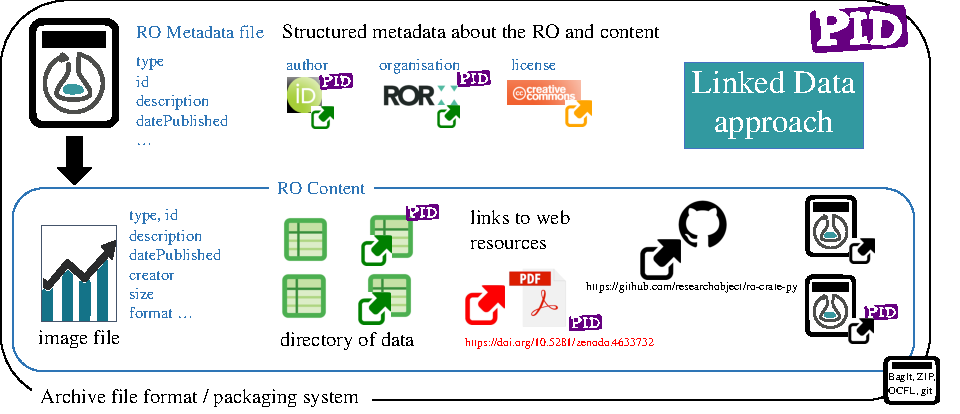
\includegraphics{content/images/ro-crate-overview.pdf}
\caption{Conceptual overview of RO-Crate. A \emph{Persistent
Identifier} (PID) \cite{doi:10.1371/journal.pbio.2001414} points to a
\emph{Research Object} (RO), which may be archived using different
packaging approaches like BagIt \cite{doi:10.17487/rfc8493}, OCFL \cite
{ocfl_2020}, git or ZIP. The RO is described within a \emph{RO-Crate
Metadata File}, providing identifiers for \emph{authors} using ORCID,
\emph{organisations} using Research Organization Registry (ROR) \cite
{doi:10.6087/kcse.192} and licences such as Creative Commons using SPDX
identifiers. The \emph{RO-Crate content} is further described with
additional metadata following a Linked Data approach. Data can be
embedded files and directories, as well as links to external Web
resources, PIDs and nested RO-Crates.}
\label{fig:conceptual}
\end{figure}

\subsubsection{Linked Data as a foundation}% {#linkeddata}

\label{sec:linkeddata}

The \textbf{Linked Data} principles \cite{doi:10.4018/978-1-60960-593-3.ch008}
(use of IRIs\footnote{\textbf{IRI}s \cite{doi:10.17487/rfc3987} are a generalisation
 of \textit{URI}s
(which include well-known http/https URLs), permitting international
Unicode characters without percent encoding, commonly used on the
browser address bar and in HTML5.} to identify resources (i.e. artefacts), resolvable via
HTTP, enriched with metadata and linked to each other) are core to
RO-Crate; therefore IRIs are used to identify an RO-Crate, its
constituent parts and metadata descriptions, and the properties and
classes used in the metadata.

RO-Crates are \textit{self-described} and follow the Linked Data principles to
describe all of their resources in both human and machine readable
manner. Hence, resources are identified using global identifiers
(absolute IRIs) where possible; and relationships between two resources
are defined with links.

The foundation of Linked Data and shared vocabularies also means that
multiple RO-Crates and other Linked Data resources can be indexed,
combined, queried, validated or transformed using existing Semantic Web
technologies such as SPARQL,\footnote{\url{https://www.w3.org/TR/sparql11-overview}}
SHACL\footnote{\url{https://www.w3.org/TR/shacl/}} and well established \textit{knowledge
graph} triple stores like Apache Jena\footnote{\url{https://jena.apache.org/}} and
OntoText GraphDB.\footnote{\url{https://www.ontotext.com/products/graphdb/}}

The possibilities of consuming\footnote{Some consideration is needed in processing of RO-Crates as
knowledge graphs, e.g. establishing absolute IRIs for files inside a
ZIP archive, detailed in the RO-Crate specification: \url
{https://www.researchobject.org/ro-crate/1.1/appendix/relative-uris.html}.} RO-Crate metadata with such
powerful tools gives another strong reason for using Linked Data as a
foundation. This use of mature Web\footnote{Note that an RO-Crate is not required to be published on the
Web, see Section~\ref{sec:selfdescribed}.} technologies also means its
developers and consumers are not restricted to the Research Object
aspects that have already been specified by the RO-Crate community, but
can extend and integrate RO-Crate in multiple standardised ways.

\subsubsection{RO-Crate is a self-described container}% {#selfdescribed}

\label{sec:selfdescribed}

An RO-Crate is defined\footnote{\url{https://www.researchobject.org/ro-crate/1.1/structure.html\#ro-crate-metadata-file-ro-crate-metadatajson}}
as a self-described \textbf{Root Data Entity} that describes and contains
\textit{data entities}, which are further described by referencing \textit{contextual
entities}. A \textbf{data entity} is either a \textit{file} (i.e. a byte sequence
stored on disk somewhere) or a \textit{directory} (i.e. set of named files and
other directories). A~file does not need to be stored inside the
RO-Crate root, it can be referenced via a PID/IRI. A \textbf{contextual
entity} exists outside the information system (e.g. a Person, a
workflow language) and is stored solely by its metadata. The
representation of a \textit{data entity} as a byte sequence makes it
possible to store a variety of research artefacts including not only
data but also, for instance, software and text.

The Root Data Entity is a directory, the \textit{RO-Crate Root}, identified by
the presence of the \textbf{RO-Crate Metadata File} \texttt{ro-crate-metadata.json}
(top of Fig.~\ref{fig:conceptual}). This file
describes the RO-Crate, its content and related metadata using Linked
Data in JSON-LD format \cite{sporny_2014}. This is a W3C standard RDF serialisation that has become
popular; it is easy to read by humans while also offering some
advantages for data exchange on the Internet. JSON-LD, a subset of the
widely supported and well-known JSON format, has tooling available for
many programming languages.\footnote{\url{https://json-ld.org/\#developers}}

The minimal requirements for the root data entity
metadata\footnote{\url{https://www.researchobject.org/ro-crate/1.1/root-data-entity.html\#direct-properties-of-the-root-data-entity}}
are \texttt{name}, \texttt{description} and \texttt{datePublished}, as well as a contextual
entity identifying its \texttt{license} -- additional metadata are commonly
added to entities depending on the purpose of the particular RO-Crate.

RO-Crates can be stored, transferred or published in multiple ways,
e.g. BagIt \cite{doi:10.17487/rfc8493}, Oxford Common File Layout
\cite{ocfl_2020} (OCFL), downloadable ZIP archives in Zenodo or through
dedicated online repositories, as well as published directly on the
Web, e.g. using GitHub Pages.\footnote{\url{https://pages.github.com/}} Combined
with Linked Data identifiers, this caters for a diverse set of storage
and access requirements across different scientific domains, from
metagenomics workflows producing hundreds of gigabytes of genome data
to cultural heritage records with access restrictions for personally
identifiable data. Specific \textit{RO-Crate profiles} (Section~\ref{sec:profiles}) may constrain serialization and publication
expectations, and require additional contextual types and properties.

\subsubsection{Data entities are described using contextual entities}% {#contextualentities}

\label{sec:contextualentities}

RO-Crate distinguishes between data and contextual
entities\footnote{\url{https://www.researchobject.org/ro-crate/1.1/contextual-entities.html\#contextual-vs-data-entities}}
in a similar way to HTTP terminology's early attempt to separate
\textit{information} (data) and \textit{non-information} (contextual) resources
\cite{httprange14}. Data entities are usually files and directories located
by relative IRI references within the RO-Crate Root, but they can also
be Web resources or restricted data identified with absolute IRIs,
including \textit{Persistent Identifiers} (PIDs) \cite{doi:10.1371/journal.pbio.2001414}.

As both types of entities are identified by IRIs, their distinction is
allowed to be blurry; data entities can be located anywhere and be
complex, while contextual entities can have a Web presence beyond their
description inside the RO-Crate. For instance
\texttt{https://orcid.org/0000-0002-1825-0097} is primarily an identifier for
a person, but secondarily it is also a Web page and a way to refer to
their academic work.

A particular IRI may appear as a contextual entity in one RO-Crate and
as a data entity in another; the distinction lies in the fact that data
entities can be considered to be \textit{contained} or captured by that
RO-Crate (\textit{RO Content} in Fig.~\ref{fig:conceptual}), while
contextual entities mainly \textit{explain} an RO-Crate or its content
(although this distinction is not a formal requirement).

In RO-Crate, a referenced contextual entity (e.g. a person identified
by ORCID) should always be described within the RO-Crate Metadata File
with at least a \textit{type} and \textit{name}, even where their PID might resolve
to further Linked Data. This is so that clients are not required to
follow every link for presentation purposes, for instance HTML
rendering. Similarly any imported extension
terms\footnote{\url{https://www.researchobject.org/ro-crate/1.1/appendix/jsonld.html\#extending-ro-crate}}
would themselves also have a human-readable description in the case
where their PID does not directly resolve to human-readable documentation.

Figure~\ref{fig:uml} shows a simplified UML class diagram of RO-Crate,
highlighting the different types of data entities and contextual
entities that can be aggregated and related. While an RO-Crate would
usually contain one or more data entities (\texttt{hasPart}), it may also be a
pure aggregation of contextual entities (\texttt{mentions}).

\begin{figure}%[t!]
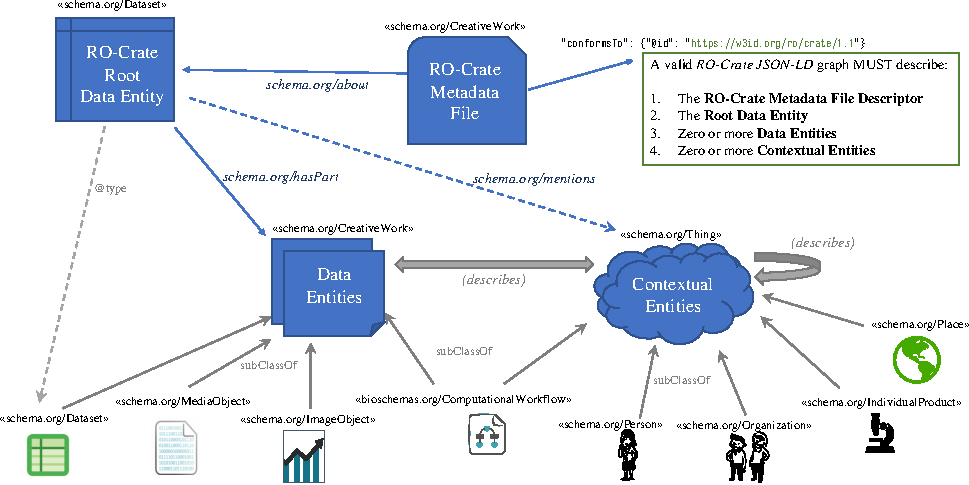
\includegraphics[width=0.9\textwidth]{content/images/ro-crate-uml.pdf}
\caption{Simplified UML class diagram of RO-Crate. The \emph
{RO-Crate Metadata File} conforms to a version of the specification;
and contains a JSON-LD graph \cite{sporny_2014} that describes the
entities that make up the RO-Crate. The \emph{RO-Crate Root Data
Entity} represent the Research Object as a dataset. The RO-Crate
aggregates \emph{data entities} (\texttt{hasPart}) which are further
described using \emph{contextual entities} (which may include
aggregated and non-aggregated data entities). Multiple types and
relations from Schema.org allow annotations to be more specific,
including figures, nested datasets, computational workflows, people,
organisations, instruments and places. Contextual entities not
otherwise cross-referenced from other entities' properties (\emph
{describes}) can be grouped under the root entity (\texttt{mentions}).}
\label{fig:uml}
\end{figure}

\subsubsection{Guide through recommended practices}% {#recommendedpractices}

\label{sec:recommendedpractices}

RO-Crate as a specification aims to build a set of recommended
practices on how to practically apply existing standards in a common
way to describe research outputs and their provenance, without having
to learn each of the underlying technologies in detail.

As such, the RO-Crate 1.1\footnote{\url{https://w3id.org/ro/crate/1.1}}
specification \cite{doi:10.5281/zenodo.4541002} can be seen as an
opinionated and example-driven guide to writing
Schema.org\footnote{\url{https://schema.org/}} \cite{doi:10.1145/2857274.2857276}
metadata as JSON-LD \cite{sporny_2014} (see Section~\ref{sec:implementation}), which leaves it open for implementers to include
additional metadata using other Schema.org types and properties, or
even additional Linked Data vocabularies/ontologies or their own ad-hoc terms.

However the primary purpose of the RO-Crate specification is to assist
developers in leveraging Linked Data principles for the focused purpose
of describing Research Objects in a structured language, while reducing
the steep learning curve otherwise associated with Semantic Web
adaptation, like development of ontologies, identifiers, namespaces,
and RDF serialization choices.
\subsubsection{Ensuring simplicity}% {#simplicity}

\label{sec:implicitly}

One aim of RO-Crate is to be conceptually simple. This simplicity has
been repeatedly checked and confirmed through an informal community
review process. For instance, in the discussion on supporting ad-hoc
vocabularies\footnote{\url{https://github.com/ResearchObject/ro-crate/issues/71}} in
RO-Crate, the community explored potential Linked Data solutions. The
conventional wisdom in RDF best
practices\footnote{\url{https://www.w3.org/TR/swbp-vocab-pub/}} is to establish a
vocabulary with a new IRI namespace, formalised using RDF
Schema\footnote{\url{http://www.w3.org/TR/2014/REC-rdf-schema-20140225/}} or
OWL\footnote{\url{http://www.w3.org/TR/2012/REC-owl2-overview-20121211/}}
ontologies. However, this may seem an excessive learning curve for
non-experts in semantic knowledge representation, and the RO-Crate
community instead agreed on a dual lightweight approach: (i)
Document\footnote{\url{https://www.researchobject.org/ro-crate/1.1/appendix/jsonld.html\#adding-new-or-ad-hoc-vocabulary-terms}}
how projects with their own Web-presence can make a pure HTML-based
vocabulary, and (ii) provide a community-wide PID namespace under
\texttt{https://w3id.org/ro/terms} that redirect to simple CSV files
maintained in GitHub.\footnote{\url{https://github.com/ResearchObject/ro-terms}}

To further verify this idea of simplicity, we have formalised the
RO-Crate definition (see \textit{Appendix~\ref{sec:formaldefinition}}). An
important result of this exercise is that the underlying data structure
of RO-Crate, although conceptually a graph, is represented as a
depth-limited tree. This formalisation also emphasises the
\textit{boundedness} of the structure; namely, the fact that elements are
specifically identified as being either semantically \textit{contained} by the
RO-Crate as \textit{Data Entities} (\texttt{hasPart}) or mainly referenced
(\texttt{mentions}) and typed as \textit{external} to the Research Object as
\textit{Contextual Entities}. It is worth pointing out that this semantic
containment can extend beyond the physical containment of files
residing within the RO-Crate Root directory on a given storage system,
as the RO-Crate data entities may include any data resource globally
identifiable using IRIs.
\subsubsection{Extensibility and RO-Crate profiles}% {#profiles}

\label{sec:profiles}

The RO-Crate specification provides a core set of conventions to
describe research outputs using types and properties applicable across
scientific domains. However we have found that domain-specific use of
RO-Crate will, implicitly or explicitly, form a specialised \textbf{profile}
of RO-Crate; i.e., {a set of conventions, types and properties that are
minimally required and one can expect to be present in that subset of
RO-Crates}. For instance, RO-Crates used for exchange of workflows will
have to contain a data entity of type \texttt{ComputationalWorkflow}, or
cultural heritage records should have a \texttt{contentLocation}.

Making such profiles explicit allow further reliable programmatic
consumption and generation of RO-Crates beyond the core types defined
in the RO-Crate specification. Following the RO-Crate mantra of
\textit{guidance over strictness}, profiles are mainly \textit{duck-typing} rather
than strict syntactic or semantic types, but may also have
corresponding machine-readable schemas at multiple levels (file
formats, JSON, RDF shapes, RDFS/OWL semantics).

The next version of the RO-Crate specification 1.2 will define a
formalization\footnote{\url{https://www.researchobject.org/ro-crate/1.2-DRAFT/profiles}}
for publishing and declaring conformance to RO-Crate profiles. Such a
profile is primarily a human-readable document of before-mentioned
expectations and conventions, but may also define a machine-readable
profile as a \textbf{Profile Crate}: Another RO-Crate that describe the
profile and in addition can list schemas for validation, compatible
software, applicable repositories, serialization/packaging formats,
extension vocabularies, custom JSON-LD contexts and examples (see for
example the Workflow RO-Crate
profile\footnote{\url{https://w3id.org/workflowhub/workflow-ro-crate/}}).

In addition, there are sometimes existing domain-specific metadata
formats, but they are either not RDF-based (and thus time-consuming to
construct terms for in JSON-LD) or are at a different granularity level
that might become overwhelming if represented directly in the RO-Crate
Metadata file (e.g. W3C PROV bundle detailing every step execution of a
workflow run \cite{doi:10.1093/gigascience/giz095}). RO-Crate allows such
\textit{alternative metadata files} to co-exist, and be described as data
entities with references to the standards and vocabularies they conform
to. This simplifies further programmatic consumption even where no
filename or file extension conventions have emerged for those metadata formats.

Section~\ref{sec:inuse} examines the observed specializations of
RO-Crate use in several domains and their emerging profiles.

\subsubsection{Technical implementation of the RO-Crate model}% {#implementation}

\label{sec:implementation}

The RO-Crate conceptual model has been realised using JSON-LD and
Schema.org in a prescriptive form as discussed in Section~\ref{sec:conceptual}. These technical choices were made to cater for
simplicity from a developer perspective (as introduced in Section~\ref{sec:methodology}).

JSON-LD\footnote{\url{https://json-ld.org/}} \cite{sporny_2014} provides a way to
express Linked Data as a JSON structure, where a \textit{context} provides
mapping to RDF properties and classes. While JSON-LD cannot map
arbitrary JSON structures to RDF, we found that it does lower the
barrier compared to other RDF syntaxes, as the JSON syntax nowadays is
a common and popular format for data exchange on the Web.

However, JSON-LD alone has too many degrees of freedom and hidden
complexities for software developers to reliably produce and consume
without specialised expertise or large RDF software frameworks. A large
part of the RO-Crate specification is therefore dedicated to describing
the acceptable subset of JSON structures.

\subsubsection{RO-Crate JSON-LD}% {#jsonld}

\label{sec:jsonld}

RO-Crate
mandates\footnote{\url{https://www.researchobject.org/ro-crate/1.1/appendix/jsonld.html}}
the use of flattened, compacted JSON-LD in the RO-Crate Metadata file
\texttt{ro-crate-metadata.json}\footnote{The avid reader may spot that the RO-Crate Metadata file use the
extension \texttt{.json} instead of \texttt{.jsonld}, this is to emphasise the
developer expectations as a JSON format, while the file's JSON-LD
nature is secondary. See \url
{https://github.com/ResearchObject/ro-crate/issues/82}.}
where a single \texttt{@graph} array contains all
the data and contextual entities in a flat list. An example can be seen
in the JSON-LD snippet in Listing \ref{lis1} below, describing a simple RO-Crate
containing data entities described using contextual entities.

\begin{listing}
%\includegraphics{210053i02}
\footnotesize
\begin{verbatim}
{ "@context": "https://w3id.org/ro/crate/1.1/context",
  "@graph": [
    { "@id": "ro-crate-metadata.json",      
      "@type": "CreativeWork",
      "conformsTo": {"@id": "https://w3id.org/ro/crate/1.1"},
      "about": {"@id": "./"}
    },
    { "@id": "./",
      "@type": "Dataset",
      "name": "A simplified RO-Crate",
      "author": {"@id": "#alice"},
      "license": {"@id": "https://spdx.org/licenses/CC-BY-4.0"},
      "datePublished": "2021-11-02T16:04:43Z",
      "hasPart": [
        {"@id": "survey-responses-2019.csv"},
        {"@id": "https://example.com/pics/5707039334816454031_o.jpg"}
      ]
    },
    { "@id": "survey-responses-2019.csv",
      "@type": "File",
      "about": {"@id": "https://example.com/pics/5707039334816454031_o.jpg"},
      "author": {"@id": "#alice"}
    },
    { "@id": "https://example.com/pics/5707039334816454031_o.jpg",
      "@type": ["File", "ImageObject"],
      "contentLocation": {"@id": "http://sws.geonames.org/8152662/"},
      "author": {"@id": "https://orcid.org/0000-0002-1825-0097"}
    },
    { "@id": "#alice",
      "@type": "Person",
      "name": "Alice"
    },
    { "@id": "https://orcid.org/0000-0002-1825-0097",
      "@type": "Person",
      "name": "Josiah Carberry"
    },
    { "@id": "http://sws.geonames.org/8152662/",
      "@type": "Place",
      "name": "Catalina Park"
    },
    { "@id": "https://spdx.org/licenses/CC-BY-4.0",
      "@type": "CreativeWork",
      "name": "Creative Commons Attribution 4.0"
    }
  ]
}    
\end{verbatim}    
\caption{%\qq{}\protect\footnotemark[31]
Simplified\protect\footnote{Recommended properties for types shown in
Listing \ref{lis1} also include
\texttt{affiliation}, \texttt{citation}, \texttt{contactPoint},
\texttt{description},
\texttt{encodingFormat}, \texttt{funder}, \texttt{geo}, \texttt{identifier},
\texttt{keywords},
\texttt{publisher}; these properties and corresponding contextual
entities are
excluded here for brevity. See complete example
\url
{https://www.researchobject.org/2021-packaging-research-artefacts-with-ro-crate/listing1/}.}
RO-Crate metadata file showing the
flattened compacted JSON-LD \texttt{@graph} array containing the data entities
and contextual entities, cross-referenced using \texttt{@id}. The
\texttt{ro-crate-metadata.json} entity self-declares conformance with the
RO-Crate specification using a versioned persistent identifier, further
RO-Crate descriptions are on the root data entity \texttt{./} or any of the
referenced data or contextual entities. This is exemplified by the data
entity \texttt{ImageObject} referencing contextual entities for
\texttt{contentLocation} and \texttt{author} that differs from that of the overall
RO-Crate. In this crate, \texttt{about} of the CSV data entity reference the
\texttt{ImageObject}, which then take the roles of both a data entity and
contextual entity. While \texttt{Person} entities ideally are identified with
ORCID PIDs as for Josiah, \texttt{\#alice} is here in contrast an RO-Crate
local identifier, highlighting the pragmatic ``just enough'' Linked
Data approach.}\label{lis1}
\end{listing}


In\footnotetext{Recommended properties for types shown in
Listing \ref{lis1} also include
\texttt{affiliation}, \texttt{citation}, \texttt{contactPoint},
\texttt{description},
\texttt{encodingFormat}, \texttt{funder}, \texttt{geo}, \texttt{identifier},
\texttt{keywords},
\texttt{publisher}; these properties and corresponding contextual
entities are
excluded here for brevity. See complete example
\url
{https://www.researchobject.org/2021-packaging-research-artefacts-with-ro-crate/listing1/}.} this flattened profile of JSON-LD, each \texttt{\{entity\}} is directly
under \texttt{@graph} and represents the RDF triples with a common \textit{subject}
(\texttt{@id}), mapped \textit{properties} like \texttt{hasPart}, and \textit{objects} -- as
either literal \texttt{"string"} values, referenced \texttt{\{objects\}} (which
properties are listed in its own entity), or a JSON \texttt{[list]} of these.
If processed as JSON-LD, this forms an RDF graph by matching the \texttt{@id}
IRIs and applying the \texttt{@context} mapping to Schema.org terms.
\normalsize

 \subsubsection{Flattened JSON-LD}

When JSON-LD 1.0 \cite{sporny_2014} was proposed, one of the motivations
was to seamlessly apply an RDF nature on top of regular JSON as
frequently used by Web APIs. JSON objects in APIs are frequently nested
with objects at multiple levels, and the perhaps most common form of
JSON-LD is the compacted
form\footnote{\url{https://json-ld.org/spec/REC/json-ld/20140116/\#compacted-document-form}}
which follows this expectation (JSON-LD
1.1\footnote{\url{https://www.w3.org/TR/2020/REC-json-ld11-20200716/}} further
expands these capabilities, e.g. allowing nested \texttt{@context} definitions).

While this feature of JSON-LD can be seen as a way to ``hide'' its RDF
nature, we found that the use of nested trees (e.g. a \texttt{Person} entity
appearing as \texttt{author} of a \texttt{File} which nests under a \texttt{Dataset} with
\texttt{hasPart}) counter-intuitively forces consumers to consider the JSON-LD
as an RDF Graph, since an identified \texttt{Person} entity can appear at
multiple and repeated points of the tree (e.g. author of multiple
files), necessitating node merging or duplication, which can become
complicated as this approach also invites the use of \textit{blank nodes}
(entities missing \texttt{@id}).

By comparison, a single flat \texttt{@graph} array approach, as required by
RO-Crate, means that applications can choose to process and edit each
entity as pure JSON by a simple lookup based on \texttt{@id}. At the same
time, lifting all entities to the same level reflects the Research
Object principles \cite{doi:10.1016/j.future.2011.08.004} in that
describing the context and provenance is just as important as
describing the data, and the requirement of \texttt{@id} of every entity
forces RO-Crate generators to consciously consider existing IRIs and
identifiers.\footnote{\url{https://www.researchobject.org/ro-crate/1.1/appendix/jsonld.html\#describing-entities-in-json-ld}}

\subsubsection{JSON-LD context}

In JSON-LD, the \texttt{@context} is a reference to another JSON-LD document
that provides mapping from JSON keys to Linked Data term IRIs, and can
enable various JSON-LD directives to cater for customised JSON
structures for translating to RDF.

RO-Crate reuses vocabulary terms and IRIs from Schema.org, but provides
its own versioned JSON-LD
context,\footnote{\url{https://w3id.org/ro/crate/1.1/context}} which has a flat list
with the mapping from JSON-LD keys to their IRI equivalents (e.g. key
\texttt{"author"} maps to the \url{http://schema.org/author} property).

The rationale behind this decision is to support JSON-based RO-Crate
applications that are largely unaware of JSON-LD, that still may want
to process the \texttt{@context} to find or add Linked Data definitions of
otherwise unknown properties and types. Not reusing the official
Schema.org context means RO-Crate is also able to map in additional
vocabularies where needed, namely the \textit{Portland Common Data Model}
(PCDM) \cite{pcdm} for repositories and Bioschemas \cite{bioschemas_2017} for
describing computational workflows. RO-Crate profiles may
extend\footnote{\url{https://www.researchobject.org/ro-crate/1.1/appendix/jsonld.html\#extending-ro-crate}}
the \texttt{@context} to re-use additional domain-specific ontologies.

Similarly, while the Schema.org context
currently\footnote{\url{https://schema.org/version/13.0/schemaorg-current-http.jsonld}}
have \texttt{"@type": "@id"} annotations for implicit object properties, RO-Crate
JSON-LD distinguishes explicitly between references to other entities
\texttt{\{"@id": "\#alice"}\}
and string values \texttt{"Alice"} -- meaning
RO-Crate applications can find references for corresponding entities
and IRIs without parsing the \texttt{@context} to understand a particular
property. Notably this is exploited by the \textit{ro-crate-html-js}
\cite{ro-crate-html-js} tool to provide reliable HTML rendering for
otherwise unknown properties and types.





\subsubsection{RO-Crate community}% {#community}

\label{sec:community}

The RO-Crate conceptual model, implementation and best practices are
developed by a growing community of researchers, developers and
publishers. RO-Crate's community is a key aspect of its effectiveness
in making research artefacts FAIR. Fundamentally, the community
provides the overall context of the implementation and model and
ensures its interoperability.

The RO-Crate community consists of:
\begin{enumerate}
\item[1.] a diverse set of people representing a variety of stakeholders;
\item[2.] a set of collective norms;
\item[3.] an open platform that facilitates communication (GitHub, Google
Docs, monthly teleconferences).
\end{enumerate}
\subsubsection{People}

The initial concept of RO-Crate was formed at the first Workshop on
Research Objects (RO2018\footnote{\url{https://www.researchobject.org/ro2018/}}),
held as part of the IEEE conference on eScience. This workshop followed
up on considerations made at a Research Data Alliance (RDA) meeting on
Research Data
Packaging\footnote{\url{https://rd-alliance.org/approaches-research-data-packaging-rda-11th-plenary-bof-meeting}}
that found similar goals across multiple data packaging efforts
\cite{doi:10.5281/zenodo.3250687}: simplicity, structured metadata and the
use of JSON-LD.

An important outcome of discussions that took place at RO2018 was the
conclusion that the original Wf4Ever Research Object ontologies
\cite{doi:10.1016/j.websem.2015.01.003}, in principle sufficient for
packaging research artefacts with rich descriptions, were, in practice,
considered inaccessible for regular programmers (e.g., Web developers)
and in danger of being incomprehensible for domain scientists due to
their reliance on Semantic Web technologies and other ontologies.

DataCrate \cite{doi:10.5281/zenodo.1445817} was presented at RO2018 as a
promising lightweight alternative approach, and an agreement was made
by a group of volunteers to attempt building what was initially called
\textit{``RO Lite''} as a combination of DataCrate's implementation and
Research Object's principles.

This group, originally made up of library and Semantic Web experts, has
subsequently grown to include domain scientists, developers, publishers
and more. This perspective of multiple views led to the specification
being used in a variety of domains, from bioinformatics and regulatory
submissions to humanities and cultural heritage preservation.

The RO-Crate community is strongly engaged with the European-wide
biology/bioinformatics collaborative e-Infrastructure ELIXIR
\cite{doi:10.1016/j.tibtech.2012.02.002}, along with European Open Science
Cloud\footnote{\url{https://eosc.eu/}} (EOSC) projects including
EOSC-Life,\footnote{\url{https://www.eosc-life.eu/}}
FAIRplus,\footnote{\url{https://fairplus-project.eu/}}
CS3MESH4EOSC\footnote{\url{https://cs3mesh4eosc.eu/}} and
BY-COVID.\footnote{\url{https://by-covid.eu/}} RO-Crate has also established
collaborations with Bioschemas \cite{bioschemas_2017}, GA4GH
\cite{doi:10.1016/j.xgen.2021.100029}, OpenAIRE \cite{rettberg_2015_openaire}
and multiple H2020 projects.

A key set of stakeholders are developers: the RO-Crate community has
made a point of attracting developers who can implement the
specifications but, importantly, keeps ``developer user experience'' in
mind. This means that the specifications are straightforward to
implement and thus do not require expertise in technologies that are
not widely deployed.

This notion of catering to ``developer user experience'' is an example
of the set of norms that have developed and now define the community.

\subsubsection{Norms}

The RO-Crate community is driven by informal conventions and notions
that are prevalent but not neccessarily written down. Here, we distil
what we as authors believe are the critical set of norms that have
facilitated the development of RO-Crate and contributed to the ability
for RO-Crate research packages to be FAIR. This is not to say that
there are no other norms within the community nor that everyone in the
community holds these uniformly. Instead, what we emphasise is that
these norms are helpful and also shaped by community practices.
\begin{enumerate}
\item[1.] Simplicity
\item[2.] Developer friendliness
\item[3.] Focus on examples and best practices rather than rigorous specification
\item[4.] Reuse ``just enough'' Web standards
\end{enumerate}

A core norm of RO-Crate is that of \textbf{simplicity}, which sets the scene
for how we guide developers to structure metadata with RO-Crate. We
focus mainly on documenting simple approaches to the most common use
cases, such as authors having an affiliation. This norm also influences
our take on \textbf{developer friendliness}; for instance, we are using the
Web-native JSON format, allowing only a few of JSON-LD's flexible
Linked Data features. Moreover, the RO-Crate documentation is largely
built up by \textbf{examples} showcasing \textbf{best practices}, rather than
rigorous specifications. We build on existing \textbf{Web standards} that
themselves are defined rigorously, which we utilise \textit{``\textbf{just
enough}''} in order to benefit from the advantages of Linked Data
(e.g., extensions by namespaced vocabularies), without imposing too
many developer choices or uncertainties (e.g., having to choose between
the many RDF syntaxes).

While the above norms alone could easily lead to the creation of ``yet
another'' JSON format, we keep the goal of \textbf{FAIR interoperability} of
the captured metadata, and therefore follow closely FAIR best practices
and current developments such as data citations, PIDs, open
repositories and recommendations for sharing research outputs and software.

\subsubsection{Open platforms}

The critical infrastructure that enables the community around RO-Crate
is the use of open development platforms. This underpins the importance
of open community access to supporting FAIR. Specifically, it is
difficult to build and consume FAIR research artefacts without being
able to access the specifications, understand how they are developed,
know about any potential implementation issues, and discuss usage to
evolve best practices.

The development of RO-Crate was driven by capturing documentation of
real-life examples and best practices rather than creating a rigorous
specification. At the same time, we agreed to be opinionated on the
syntactic form to reduce the jungle of implementation choices; we
wanted to keep the important aspects of Linked Data to adhere to the
FAIR principles while retaining the option of combining and extending
the structured metadata using the existing Semantic Web stack, not just
build a standalone JSON format.

Further work during 2019 started adapting the DataCrate documentation
through a more collaborative and exploratory \textit{RO Lite} phase, initially
using Google Docs for review and discussion, then moving to GitHub as a
collaboration space for developing what is now the RO-Crate
specification, maintained\footnote{\url{https://github.com/researchobject/ro-crate/}} as
Markdown in GitHub Pages
and published through Zenodo.

In addition to the typical Open Source-style development with GitHub
issues and pull requests, the RO-Crate Community have, at time of
writing, two regular monthly calls, a Slack channel and a mailing list
for coordinating the project; also many of its participants collaborate
on RO-Crate at multiple conferences and coding events such as the
ELIXIR BioHackathon.\footnote{\url{https://biohackathon-europe.org/}} The community
is jointly developing the RO-Crate specification and Open Source tools,
as well as providing support and considering new use cases. The
RO-Crate Community\footnote{\url{https://www.researchobject.org/ro-crate/community}}
is open for anyone to join, to equally participate under a code of
conduct, and as of October 2021 has more than 50 members (see Appendix~\ref{sec:communitylist}).

% Please update in 31.tooling-table.md first!
%
\begin{table}[t!]%[htbp]
\tabcolsep=0pt
\caption{Applications and libraries implementing RO-Crate, targeting
different types of users across multiple programming languages. Status
is indicative as assessed by this work (Alpha $<$ Beta $<$ Release
Candidate (RC) $<$ Release)}
\label{tab1}
%
\begin{tabular*}{\textwidth}{@{\extracolsep{4in minus 4in}}llcc@{}}
\hline
\textbf{Tool name} & \multicolumn{1}{c}{\multirow{2}{*}{Targets}}
& \multirow{2}{*}{Language/Platform} & \multirow{2}{*}{Status} \\
\textit{Brief Description}&&& \\
\hline
\textbf{Describo} \cite{describo}                                                                                                          & Research Data Managers     & NodeJS (Desktop) & RC    \\
\multicolumn{4}{@{}l@{}}{\textit{Interactive desktop application to create, update and export RO-Crates for different profiles}}                                                                               \\
\textbf{Describo Online} \cite{describo-online}                                                                                            & Platform developers        & NodeJS (Web)     & Alpha \\
\multicolumn{4}{@{}l@{}}{\textit{Web-based application to create RO-Crates using cloud storage}}                                                                                                               \\
\textbf{ro-crate-excel} \cite{ro-crate-excel}                                                                                              & Data managers              & JavaScript       & Beta  \\
\multicolumn{4}{@{}l@{}}{\textit{Command-line tool to create/edit RO-Crates with spreadsheets}}                                                                                                                \\
\textbf{ro-crate-html-js} \cite{ro-crate-html-js}                                                                                          & Developers                 & JavaScript       & Beta  \\
\multicolumn{4}{@{}l@{}}{\textit{HTML rendering of RO-Crate}}                                                                                                                                                  \\
\textbf{ro-crate-js} \cite{ro-crate-js}                                                                                                    & Research Data Managers     & JavaScript       & Alpha \\
\multicolumn{4}{@{}l@{}}{\textit{Library for creating/manipulating crates; basic validation code}}                                                                                                             \\
\textbf{ro-crate-ruby} \cite{ro-crate-ruby}                                                                                                & Developers                 & Ruby             & Beta  \\
\multicolumn{4}{@{}l@{}}{\textit{Ruby library for reading/writing RO-Crate, with workflow support}}                                                                                                            \\
\textbf{ro-crate-py} \cite{ro-crate-py}                                                                                                    & Developers                 & Python           & Beta  \\
\multicolumn{4}{@{}l@{}}{\textit{Object-oriented Python library for reading/writing RO-Crate and use by Jupyter Notebook}}                                                                                     \\
\textbf{WorkflowHub} \cite{about-workflowhub}                                                                                              & Workflow users             & Ruby             & Beta  \\
\multicolumn{4}{@{}l@{}}{\textit{Workflow repository; imports and exports Workflow RO-Crate}}                                                                                                                  \\
\textbf{Life Monitor} \cite{about-lifemonitor}                                                                                             & Workflow developers        & Python           & Alpha \\
\multicolumn{4}{@{}l@{}}{\textit{Workflow testing and monitoring service; Workflow Testing profile of RO-Crate}}                                                                                               \\
\textbf{SCHeMa} \cite{vergoulis2021schema}                                                                                                 & Workflow users             & PHP              & Alpha \\
\multicolumn{4}{@{}l@{}}{\textit{Workflow execution using RO-Crate as exchange mechanism}}                                                                                                                     \\
\textbf{galaxy2cwl} \cite{galaxy2cwl}                                                                                                      & Workflow developers        & Python           & Alpha \\
\multicolumn{4}{@{}l@{}}{\textit{Wraps Galaxy workflow as Workflow RO-Crate}}                                                                                                                                  \\
\textbf{Modern PARADISEC} \cite{modpdsc}                                                                                                   & Repository managers        & Platform         & Beta  \\
\multicolumn{4}{@{}l@{}}{\textit{Cultural Heritage portal based on OCFL and RO-Crate}}                                                                                                                        \\
\textbf{ONI express} \cite{arkisto-data-portal}                                                                                            & Repository managers        & Platform         & Beta  \\
\multicolumn{4}{@{}l@{}}{\textit{Platform for publishing data and documents stored in an OCFL repository via a Web interface}}                                                                                 \\
\textbf{ocfl-tools} \cite{ocfl-tools}                                                                                                      & Developers                 & JavaScript (CLI) & Beta  \\
\multicolumn{4}{@{}l@{}}{\textit{Tools for managing RO-Crates in an OCFL repository}}                                                                                                                          \\
\textbf{RO Composer} \cite{ro-composer}                                                                                                    & Repository developers      & Java             & Alpha \\
\multicolumn{4}{@{}l@{}}{\textit{REST API for gradually building ROs for given profile}}                                                                                                                       \\
\textbf{RDA maDMP Mapper} \cite{doi:10.5281/zenodo.3922136}                                                                                & Data Management Plan users & Python           & Beta  \\
\multicolumn{4}{@{}l@{}}{\textit{Mapping between machine-actionable data management plans (maDMP) and RO-Crate \cite{doi:10.4126/frl01-006423291}}}                                                         \\
\textbf{Ro-Crate\_2\_ma-DMP} \cite{doi:10.5281/zenodo.3903463}                                                                             & Data Management Plan users & Python           & Beta  \\
\multicolumn{4}{@{}l@{}}{\textit{Convert between machine-actionable data management plans (maDMP) and RO-Crate}}                                                                                              \\
\textbf{CheckMyCrate} \cite{CheckMyCrate}                                                                                                  & Developers                 & Python (CLI)     & Alpha \\
\multicolumn{4}{@{}l@{}}{\textit{Validation according to Workflow RO-Crate profile}}                                                                                                                           \\
\textbf{RO-Crates-and-Excel} \cite{doi:10.5281/zenodo.5068950}                                                                             & Data Managers              & Java (CLI)       & Alpha \\
\multicolumn{4}{@{}l@{}}{\textit{Describe column/data details of spreadsheets as RO-Crate using DataCube vocabulary}}                                                                                          \\
\hline
\end{tabular*}\vspace*{10pt}
\end{table}


\subsection{RO-Crate tooling}% {#tooling}

\label{sec:tooling}

The work of the community has led to the development of a number of
tools for creating and using RO-Crates. Table~\ref{tab1} shows the current set
of implementations. Reviewing this list, one can see support for
commonly used programming languages, including Python, JavaScript, and
Ruby. Additionally, the tools can be integrated into commonly used
research environments, in particular, the command line tool
\textit{ro-crate-html-js} \cite{ro-crate-html-js} for creating a human-readable
preview of an RO-Crate as a sidecar HTML file. Furthermore, there are
tools that cater to end-users (\textit{Describo} \cite{describo}, \textit{WorkflowHub}
\cite{about-workflowhub}), in order to simplify creating and managing
RO-Crate. For example, Describo was developed to help researchers of
the Australian Criminal Characters
project\footnote{\url{https://criminalcharacters.com/}} to annotate historical prisoner
records for greater insight into the history of Australia
\cite{doi:10.1080/14490854.2020.1796500}.

While the development of these tools is promising, our analysis of
their maturity status shows that the majority of them are in the Beta
stage. This is partly due to the fact that the RO-Crate specification
itself only recently reached 1.0 status, in November 2019
\cite{doi:10.5281/zenodo.3541888}. Now that there is a fixed point of
reference: With version 1.1 (October 2020)
\cite{doi:10.5281/zenodo.4031327} RO-Crate has stabilised based on feedback
from application development, and now we are seeing a further increase
in the maturity of these tools, along with the creation of new ones.

Given the stage of the specification, these tools have been primarily
targeting developers, essentially providing them with the core
libraries for working with RO-Crate. Another target has been that of
research data managers who need to manage and curate large amounts of data.

\subsection{Profiles of RO-Crate in use}% {#inuse}

\label{sec:inuse}

RO-Crate fundamentally forms part of an infrastructure to help build
FAIR research artefacts. In other words, the key question is whether
RO-Crate can be used to share and (re)use research artefacts. Here we
look at three research domains where RO-Crate is being applied:
Bioinformatics, Regulatory Science and Cultural Heritage. In addition,
we note how RO-Crate may have an important role as part of
machine-actionable data management plans and institutional repositories.

From these varied uses of RO-Crate we observe natural differences in
their detail level and the type of entities described by the RO-Crate.
For instance, on submission of an RO-Crate to a workflow repository, it
is reasonable to expect the RO-Crate to contain at least one workflow,
ideally with a declared licence and workflow language. Specific
additional recommendations such as on identifiers is also needed to
meet the emerging requirements of FAIR Digital
Objects.\footnote{\url{https://fairdo.org/}} Work has now
begun\footnote{\url{https://github.com/ResearchObject/ro-crate/issues/153}} to
formalise these different \textit{profiles} of RO-Crates, which may impose
additional constraints based on the needs of a specific domain or use case.

\subsubsection{Bioinformatics workflows}% {#workflows}

\label{sec:workflows}

WorkflowHub.eu\footnote{\url{https://workflowhub.eu/}} is a European cross-domain
registry of computational workflows, supported by European Open Science
Cloud projects, e.g. EOSC-Life,\footnote{\url{https://www.eosc-life.eu/}} and
research infrastructures including the pan-European bioinformatics
network ELIXIR\footnote{\url{https://elixir-europe.org/}}
\cite{doi:10.1016/j.tibtech.2012.02.002}. As part of promoting workflows as
reusable tools, WorkflowHub includes documentation and high-level
rendering of the workflow structure independent of its native workflow
definition format. The rationale is that a domain scientist can browse
all relevant workflows for their domain, before narrowing down their
workflow engine requirements. As such, the WorkflowHub is intended
largely as a registry of workflows already deposited in repositories
specific to particular workflow languages and domains, such as
UseGalaxy.eu \cite{doi:10.1371/journal.ppat.1008643} and Nextflow nf-core
\cite{doi:10.1038/s41587-020-0439-x}.

We here describe three different RO-Crate profiles developed for use
with WorkflowHub.

\subsubsection{Profile for describing workflows}

Being cross-domain, WorkflowHub has to cater for many different
workflow systems. Many of these, for instance Nextflow
\cite{doi:10.1038/nbt.3820} and Snakemake
\cite{doi:10.1093/bioinformatics/bts480}, by virtue of their script-like
nature, reference multiple neighbouring files typically maintained in a
GitHub repository. This calls for a data exchange method that allows
keeping related files together. WorkflowHub has tackled this problem by
adopting RO-Crate as the packaging mechanism
\cite{doi:10.5281/zenodo.4705078}, typing and annotating the constituent
files of a workflow and -- crucially -- marking up the workflow
language, as many workflow engines use common file extensions like
\texttt{*.xml} and \texttt{*.json}. Workflows are further described with authors,
license, diagram previews and a listing of their inputs and outputs.
RO-Crates can thus be used for interoperable deposition of workflows to
WorkflowHub, but are also used as an archive for downloading workflows,
embedding metadata registered with the WorkflowHub entry and translated
workflow files such as abstract Common Workflow Language (CWL)
\cite{doi:10.1145/3486897} definitions and diagrams \cite{doi:10.5281/zenodo.4605654}.

RO-Crate acts therefore as an interoperability layer between
registries, repositories and users in WorkflowHub. The iterative
development between WorkflowHub developers and the RO-Crate community
heavily informed the creation of the Bioschemas \cite{bioschemas_2017}
profile for Computational
Workflows,\footnote{\url{https://bioschemas.org/profiles/ComputationalWorkflow/1.0-RELEASE/}}
which again informed the RO-Crate 1.1 specification on
workflows\footnote{\url{https://www.researchobject.org/ro-crate/1.1/workflows.html}}
and led to the RO-Crate Python library \cite{ro-crate-py} and WorkflowHub's
\textbf{Workflow RO-Crate
profile},\footnote{\url{https://w3id.org/workflowhub/workflow-ro-crate/1.0}} which,
in a similar fashion to RO-Crate itself, recommends which workflow
resources and descriptions are required. This co-development across
project boundaries exemplifies the drive for simplicity and for
establishing best practices.

\subsubsection{Profile for recording workflow runs}

RO-Crates in WorkflowHub have so far been focused on workflows that are
ready to be run, and development of WorkflowHub is now creating a
\textbf{Workflow Run RO-Crate profile} for the purposes of benchmarking,
testing and executing workflows. As such, RO-Crate serves as a
container of both a \textit{workflow definition} that may be executed and of a
particular \textit{workflow execution with test results}.

This workflow run profile is a continuation of our previous work with
capturing workflow provenance in a Research Object in CWLProv
\cite{doi:10.1093/gigascience/giz095} and TavernaPROV
\cite{doi:10.5281/zenodo.51314}. In both cases, we used the PROV Ontology
\cite{PROVO}, including details of every task execution with all the
intermediate data, which required significant workflow engine
integration.\footnote{CWLProv and TavernaProv predate RO-Crate, but use
RO-Bundle\cite{doi:10.5281/zenodo.12586}, a similar Research Object
packaging method with JSON-LD metadata.}

Simplifying from the CWLProv approach, the planned Workflow Run
RO-Crate profile will use a high level Schema.org
provenance\footnote{\url{https://www.researchobject.org/ro-crate/1.1/provenance.html\#software-used-to-create-files}}
for the input/output boundary of the overall workflow execution. This
\textit{Level 1 workflow provenance} \cite{doi:10.1093/gigascience/giz095} can be
expressed generally across workflow languages with minimal workflow
engine changes, with the option of more detailed provenance traces as
separate PROV artefacts in the RO-Crate as data entities. In the
current development of Specimen Data
Refinery\footnote{\url{https://github.com/DiSSCo/SDR}} \cite{doi:10.3897/rio.6.e57602}
these RO-Crates will document the text recognition workflow runs of
digitised biological specimens, exposed as FAIR Digital Objects
\cite{doi:10.3390/publications8020021}.

WorkflowHub has recently enabled minting of Digital Object Identifiers
(DOIs), a PID commonly used for scholarly artefacts, for registered
workflows, e.g. \texttt{10.48546/workflowhub.workflow.56.1}
\cite{doi:10.48546/workflowhub.workflow.56.1}, lowering the barrier for
citing workflows as computational methods along with their FAIR
metadata -- captured within an RO-Crate. While it is not an aim for
WorkflowHub to be a repository of workflow runs and their data,
RO-Crates of \textit{exemplar workflow runs} serve as useful workflow
documentation, as well as being an exchange mechanism that preserves
FAIR metadata in a diverse workflow execution environment.

\subsubsection{Profile for testing workflows}

The value of computational workflows, however, is potentially
undermined by the ``collapse'' over time of the software and services
they depend upon: for instance, software dependencies can change in a
non-backwards-compatible manner, or active maintenance may cease; an
external resource, such as a reference index or a database query
service, could shift to a different URL or modify its access protocol;
or the workflow itself may develop hard-to-find bugs as it is updated.
This \textit{workflow decay} can take a big toll on the workflow's reusability
and on the reproducibility of any processes it evokes
\cite{doi:10.1109/eScience.2012.6404482}.

For this reason, WorkflowHub is complemented by a monitoring and
testing service called LifeMonitor \cite{about-lifemonitor}, also supported
by EOSC-Life. LifeMonitor's main goal is to assist in the creation,
periodic execution and monitoring of workflow tests, enabling the early
detection of software collapse in order to minimise its detrimental
effects. The communication of metadata related to workflow testing is
achieved through the adoption of a \textbf{Workflow Testing RO-Crate
profile}\footnote{\url{https://lifemonitor.eu/workflow_testing_ro_crate}} stacked on
top of the \textit{Workflow RO-Crate} profile. This further specialisation of
Workflow RO-Crate allows to specify additional testing-related entities
(test suites, instances, services, etc.), leveraging RO-Crate's
extension
mechanism\footnote{\url{https://www.researchobject.org/ro-crate/1.1/appendix/jsonld.html\#extending-ro-crate}}
through the addition of terms from custom namespaces.

In addition to showcasing RO-Crate's extensibility, the testing profile
is an example of the format's flexibility and adaptability to the
different needs of the research community. Though ultimately related to
a computational workflow, in fact, most of the testing-specific
entities are more about describing a protocol for interacting with a
monitoring service than a set of research outputs and its associated
metadata. Indeed, one of LifeMonitor's main functionalities is
monitoring and reporting on test suites running on existing Continuous
Integration (CI) services, which is described in terms of service URLs
and job identifiers in the testing profile. In principle, in this
context, data could disappear altogether, leading to an RO-Crate
consisting entirely of contextual entities. Such an RO-Crate acts more
as an exchange format for communication between services (WorkflowHub
and LifeMonitor) than as an aggregator for research data and metadata,
providing a good example of the format's high versatility.


\subsubsection{Regulatory sciences}% {#regulatorysciences}

\label{sec:regulatorysciences}

BioCompute Objects\footnote{\url{https://biocomputeobject.org/}} (BCO)
\cite{doi:10.1371/journal.pbio.3000099} is a community-led effort to
standardise submissions of computational workflows to biomedical
regulators. For instance, a genomics sequencing pipeline, as part of a
personalised cancer treatment study, can be submitted to the US Food
and Drugs Administration (FDA) for approval. BCOs are formalised in the
standard IEEE 2791-2020 \cite{doi:10.1109/IEEESTD.2020.9094416} as a
combination of JSON
Schemas\footnote{\url{https://w3id.org/ieee/ieee-2791-schema/}}
that define the structure of JSON metadata files describing exemplar
workflow runs in detail, covering aspects such as the usability and
error domain of the workflow, its runtime requirements, the reference
datasets used and representative output data produced.

BCOs provide a structured view over a particular workflow, informing
regulators about its workings independently of the underlying workflow
definition language. However, BCOs have only limited support for
additional metadata.\footnote{IEEE 2791-2020 do permit user extensions in the \textit{extension
domain} by referencing additional JSON Schemas.} For instance, while the BCO itself can
indicate authors and contributors, and in particular regulators and
their review decisions, it cannot describe the provenance of individual
data files or workflow definitions.

As a custom JSON format, BCOs cannot be extended with Linked Data
concepts, except by adding an additional top-level JSON object
formalised in another JSON Schema. A BCO and workflow submitted by
upload to a regulator will also frequently consist of multiple
cross-related files. Crucially, there is no way to tell whether a given
\texttt{*.json} file is a BCO file, except by reading its content and check
for its \texttt{spec\_version}.

We can then consider how a BCO and its referenced artefacts can be
packaged and transferred following FAIR principles. \textbf{BCO
RO-Crate}\footnote{\url{https://biocompute-objects.github.io/bco-ro-crate/}} \cite{doi:10.5281/zenodo.4633732},
part of the BioCompute Object user guides, defines a set of best
practices for wrapping a BCO with a workflow, together with its
exemplar outputs in an RO-Crate, which then provides typing and
additional provenance metadata of the individual files, workflow
definition, referenced data and the BCO metadata itself.

Here the BCO is responsible for describing the \textit{purpose} of a workflow
and its run at an abstraction level suitable for a domain scientist,
while the more open-ended RO-Crate describes the surroundings of the
workflow, classifying and relating its resources and providing
provenance of their existence beyond the BCO. This emerging \textit{separation
of concerns} is shown in Fig.~\ref{fig:sep_concerns}, and highlights
how RO-Crate is used side-by-side of existing standards and tooling,
even where there are apparent partial overlaps.

A similar separation of concerns can be found if considering the
RO-Crate as a set of files, where the \textit{transport-level} metadata, such
as checksum of files, are delegated to separate
BagIt\footnote{\url{https://www.researchobject.org/ro-crate/1.1/appendix/implementation-notes.html\#adding-ro-crate-to-bagit}}
manifests, a standard focusing on the preservation challenges of
digital libraries \cite{doi:10.17487/rfc8493}. As such, RO-Crate metadata
files are not required to iterate all the files in their folder
hierarchy, only those that benefit from being described.

Specifically, a BCO description alone is insufficient for reliable
re-execution of a workflow, which would need a compatible workflow
engine depending on the original workflow definition language, so IEEE
2791 recommends using Common Workflow Language (CWL)
\cite{doi:10.1145/3486897} for interoperable pipeline execution. CWL itself
relies on tool packaging in software containers using
Docker\footnote{\url{https://www.docker.com/}} or Conda.\footnote{\url{https://docs.conda.io/}}
Thus, we can consider BCO RO-Crate as a stack: transport-level
manifests of files (BagIt), provenance, typing and context of those
files (RO-Crate), workflow overview and purpose (BCO), interoperable
workflow definition (CWL) and tool distribution (Docker).

%
\begin{figure}%[t]
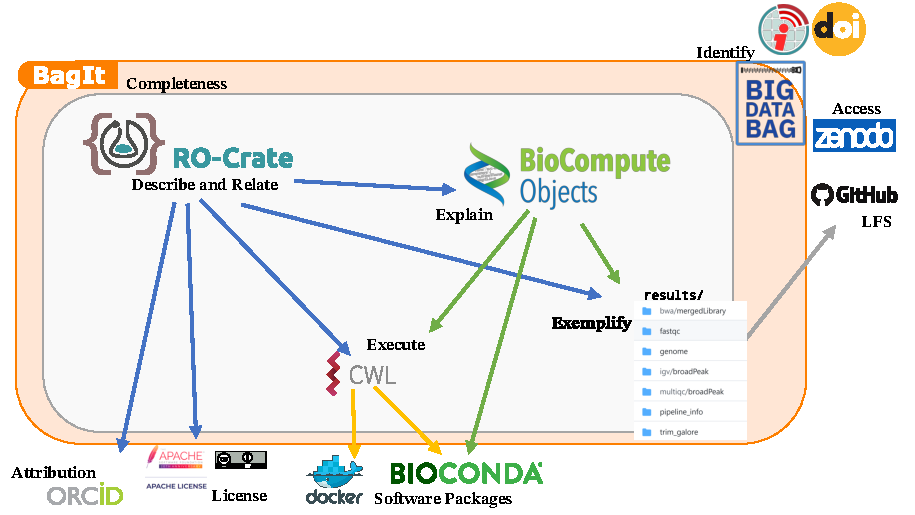
\includegraphics{content/images/ro-crate-bco-sep-of-concerns.pdf}
\caption{Separation of Concerns in BCO RO-Crate. BioCompute
Object (IEEE2791) is a JSON file that structurally explains the purpose
and implementation of a computational workflow, for instance
implemented in Common Workflow Language (CWL), that installs the
workflow's software dependencies as Docker containers or BioConda
packages. An example execution of the workflow shows the different
kinds of result outputs, which may be external, using GitHub LFS \cite
{github-lfs} to support larger data. RO-Crate gathers all these local
and external resources, relating them and giving individual
descriptions, for instance permanent DOI identifiers for reused
datasets accessed from Zenodo, but also adding external identifiers to
attribute authors using ORCID or to identify which licences apply to
individual resources. The RO-Crate and its local files are captured in
a BagIt whose checksum ensures completeness, combined with Big Data Bag
\cite{doi:10.1109/BigData.2016.7840618} features to ``complete'' the
bag with large external files such as the workflow outputs.}
\label{fig:sep_concerns}
\end{figure}
%
\subsubsection{Digital humanities: Cultural heritage}% {#culturalheritage}

\label{sec:culturalheritage}

The Pacific And Regional Archive for Digital Sources in Endangered
Cultures (PARADISEC\footnote{\url{https://www.paradisec.org.au/}}) \cite{doi:10125/4567}
maintains a repository of more than 500,000 files documenting
endangered languages across more than 16,000 items, collected and
digitised over many years by researchers interviewing and recording
native speakers across the region.

The Modern PARADISEC demonstrator\footnote{\url{https://mod.paradisec.org.au/}} has
been
proposed\footnote{\url{https://arkisto-platform.github.io/case-studies/paradisec/}}
as an update to the 18 year old infrastructure, to also help long-term
preservation of these artefacts in their digital form. The demonstrator
uses RO-Crate to describe the overall structure and to capture the
metadata of each item. The existing PARADISEC data collection has been
ported and captured as RO-Crates. A Web portal then exposes the
repository and its entries by indexing the RO-Crate metadata files,
presenting a domain-specific view of the items -- the RO-Crate is
``hidden'' and does not change the user interface.

The PARADISEC use case takes advantage of several RO-Crate features and
principles. Firstly, the transcribed metadata are now independent of
the PARADISEC platform and can be archived, preserved and processed in
its own right, using Schema.org as base vocabulary and extended with
PARADISEC-specific terms.

In this approach, RO-Crate is the holder of itemised metadata, stored
in regular files that are organised using Oxford Common File
Layout\footnote{\url{https://ocfl.io/1.0/spec/}} (OCFL) \cite{ocfl_2020}, which ensures
file integrity and versioning on a regular shared file system. This
lightweight infrastructure also gives flexibility for future
developments and maintenance. For example a consumer can use Linked
Data software such as a graph database and query the whole corpora
using SPARQL triple patterns across multiple RO-Crates. For long term
digital preservation, beyond the lifetime of PARADISEC portals, a
``last resort'' fallback is storing the generic RO-Crate HTML preview
\cite{ro-crate-html-js}. Such human-readable rendering of RO-Crates can be
hosted as static files by any Web server, in line with the approach
taken by the Endings Project.\footnote{The Endings Project \url{https://endings.uvic.ca/} is a five-year
project funded by the Social Sciences and Humanities Research Council
(SSHRC) that is creating tools, principles, policies and
recommendations for digital scholarship practitioners to create
accessible, stable, long-lasting resources in the humanities.}

\subsubsection{Machine-actionable Data Management Plans}% {#dmp}

\label{sec:dmp}

Machine-actionable Data Management Plans (maDMPs) have been proposed as
an improvement to automate FAIR data management tasks in research
\cite{doi:10.1371/journal.pcbi.1006750}; maDMPs use PIDs and controlled
vocabularies to describe what happens to data over the research life
cycle \cite{doi:10.1007/978-3-030-45442-5_15}. The Research Data Alliance's
\textit{DMP Common Standard} for maDMPs \cite{doi:10.15497/rda00039} is one such
formalisation for expressing maDMPs, which can be expressed as Linked
Data using the DMP Common Standard Ontology
\cite{doi:10.4126/frl01-006423289}, a specialisation of the W3C Data
Catalog Vocabulary (DCAT) \cite{dcat2}. RDA maDMPs are usually expressed
using regular JSON, conforming to the DMP JSON Schema.

A mapping has been produced between Research Object Crates and
Machine-actionable Data Management Plans
\cite{doi:10.4126/frl01-006423291}, implemented by the RO-Crate RDA maDMP
Mapper \cite{doi:10.5281/zenodo.3922136}. A similar mapping has been
implemented by \textit{RO-Crate\_2\_ma-DMP} \cite{doi:10.5281/zenodo.3903463}. In
both cases, a maDMP can be converted to a RO-Crate, or vice versa. In
\cite{doi:10.4126/frl01-006423291} this functionality caters for two use cases:
\begin{enumerate}
\item[1.] Start a skeleton data management plan based on an existing RO-Crate
dataset, e.g. an RO-Crate from WorkflowHub.
\item[2.] Instantiate an RO-Crate based on a data management plan.
\end{enumerate}

An important nuance here is that data management plans are (ideally)
written in \textit{advance} of data production, while RO-Crates are typically
created to describe data \textit{after} it has been generated. What is
significant to note in this approach is the importance of
\textbf{templating} in order to make both tasks automatable and achievable,
and how RO-Crate can fit into earlier stages of the research life cycle.
\subsubsection{Institutional data repositories -- Harvard Data Commons}% {#institutionalrepos}

\label{sec:institutionalrepos}

The concept of a \textbf{Data Commons} for research collaboration was
originally defined as \textit{``cyber-infrastructure that co-locates data,
storage, and computing infrastructure with commonly used tools for
analysing and sharing data to create an interoperable resource for the
research community''} \cite{doi:10.1109/MCSE.2016.92}. More recently, Data
Commons has been established to mean integration of active
data-intensive research with data management and archival best
practices, along with a supporting computational infrastructure.
Furthermore, the Commons features tools and services, such as
computation clusters and storage for scalability, data repositories for
disseminating and preserving regular, but also large or sensitive
datasets, and other research assets. Multiple initiatives were
undertaken to create Data Commons on national, research, and
institutional levels. For example, the Australian Research Data
Commons (ARDC)\footnote{\url{https://ardc.edu.au/}} \cite{doi:10.5334/dsj-2019-044} is a
national initiative that enables local researchers and industries to
access computing infrastructure, training, and curated datasets for
data-intensive research. NCI's Genomic Data
Commons\footnote{\url{https://gdc.cancer.gov/}} (GDC)
\cite{doi:10.1182/blood-2017-03-735654} provides the cancer research
community with access to a vast volume of genomic and clinical data.
Initiatives such as Research Data Alliance (RDA) Global Open Research
Commons\footnote{\url{https://www.rd-alliance.org/groups/global-open-research-commons-ig}}
propose standards for the implementation of Data Commons to prevent
them becoming ``data silos'' and thus, enable interoperability from one
Data Commons to another.

\textbf{Harvard Data Commons} \cite{doi:10.7557/5.5422} aims to address the
challenges of data access and cross-disciplinary research within a
research institution. It brings together multiple institutional
schools, libraries, computing centres and the Harvard
Dataverse\footnote{\url{https://dataverse.harvard.edu/}} data repository.
Dataverse\footnote{\url{https://dataverse.org/}} \cite{doi:10.1045/january2011-crosas}
is a free and open-source software platform to archive, share and cite
research data. The Harvard Dataverse repository is the largest of 70
Dataverse installations worldwide, containing over 120K datasets with
about 1.3M data files (as of 2021-11-16). Working toward the goal of
facilitating collaboration and data discoverability and management
within the university, Harvard Data Commons has the following primary
objectives:\looseness=1
\begin{enumerate}
\item[1.] the integration of Harvard Research Computing with Harvard Dataverse
by leveraging Globus endpoints \cite{doi:10.1109/MCC.2014.52}; this will
allow an automatic transfer of large datasets to the repository. In
some cases, only the metadata will be transferred while the data stays
stored in remote storage;
\item[2.] support for advanced research workflows and providing packaging
options for assets such as code and workflows in the Harvard Dataverse
repository to enable reproducibility and reuse, and
\item[3.] interation of repositories supported by Harvard, which include
DASH,\footnote{\url{https://dash.harvard.edu/}} the open access institutional
repository, the Digital Repository Services (DRS) for preserving
digital asset collections, and the Harvard Dataverse.
\end{enumerate}

Particularly relevant to this article is the second objective of the
Harvard Data Commons, which aims to support the deposit of research
artefacts to Harvard Dataverse with sufficient information in the
metadata to allow their future reuse (Fig.~\ref{fig:hdc}). To support
the incorporation of data, code, and other artefacts from various
institutional infrastructures, Harvard Data Commons is currently
working on RO-Crate adaptation. The RO-Crate metadata provides the
necessary structure to make all research artefacts FAIR. The Dataverse
software already has extensive support for metadata\footnote{\url{https://guides.dataverse.org/en/latest/user/appendix.html}}, including the Data
Documentation Initiative (DDI), Dublin Core, DataCite, and Schema.org.
Incorporating RO-Crate, which has the flexibility to describe a wide
range of research resources, will facilitate their seamless transition
from one infrastructure to the other within the Harvard Data Commons.

Even though the Harvard Data Commons is specific to Harvard University,
the overall vision and the three objectives can be abstracted and
applied to other universities or research organisations. The Commons
will be designed and implemented using standards and commonly-used
approaches to make it interoperable and reusable by others.

\begin{figure}%[t!]
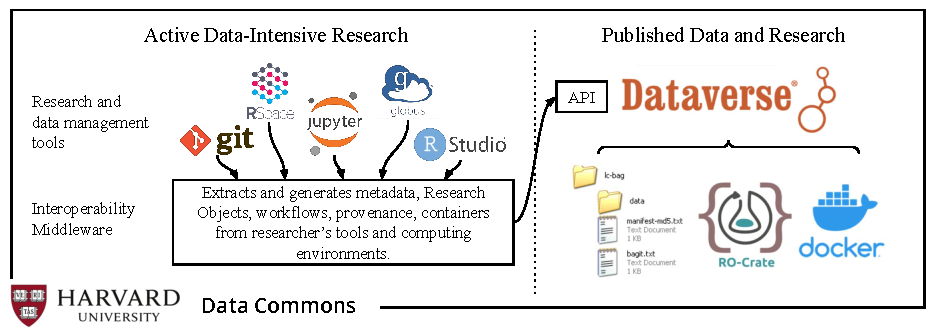
\includegraphics{content/images/data-commons-ro-crate-figure-5.pdf}
\caption{One aspect of Harvard Data Commons. Automatic
encapsulation and deposit of artefacts from data management tools used
during active research at the Harvard Dataverse repository.}
\label{fig:hdc}
\end{figure}

 \subsection{Related work}% {#relatedwork}

\label{sec:relatedwork}

With the increasing digitisation of research processes, there has been
a significant call for the wider adoption of interoperable sharing of
data and its associated metadata. We refer to
\cite{doi:10.1016/j.patter.2020.100136} for a comprehensive overview and
recommendations, in particular for data; notably that review highlights
the wide variety of metadata and documentation that the literature
prescribes for enabling data reuse. Likewise, we suggest
\cite{doi:10.1016/j.patter.2021.100322} that covers the importance of
metadata standards in reproducible computational research.

Here we focus on approaches for bundling research artefacts along with
their metadata. This notion of publishing compound objects for
scholarly communication has a long history behind it
\cite{doi:10.1190/1.1822162,vandesompel_2007}, but recent approaches
have followed three main strands: (1) publishing to centralised
repositories; (2) packaging approaches similar to RO-Crate; and (3)
bundling the computational workflow around a scientific experiment.

 \subsubsection{Bundling and packaging digital research artefacts}

Early work making the case for publishing compound scholarly
communication units \cite{vandesompel_2007} led to the development of the
Object Re-Use and Exchange
model\footnote{\url{http://www.openarchives.org/ore/1.0/primer}} (OAI-ORE), providing
a structured \textbf{resource map} of the digital artefacts that together
support a scholarly output.

The challenge of describing computational workflows was one of the main
motivations for the early proposal of \textit{Research Objects} (RO)
\cite{doi:10.1016/j.future.2011.08.004} as first-class citizens for sharing
and publishing. The RO approach involves bundling datasets, workflows,
scripts and results along with traditional dissemination materials like
journal articles and presentations, forming a single package.
Crucially, these resources are not just gathered, but also individually
typed, described and related to each other using semantic vocabularies.
As pointed out in \cite{doi:10.1016/j.future.2011.08.004} an open-ended
\textit{Linked Data} approach is not sufficient for scholarly communication: a
common data model is also needed in addition to common and best
practices for managing and annotating lifecycle, ownership, versioning
and attributions.

Considering the FAIR principles \cite{doi:10.1038/sdata.2016.18}, we can
say with hindsight that the initial RO approaches strongly targeted
\textit{Interoperability}, with a particular focus on the reproducibility of
\textit{in-silico experiments} involving computational workflows and the reuse
of existing RDF vocabularies.

The first implementation of Research Objects for sharing workflows in
myExperiment \cite{doi:10.1093/nar/gkq429} was based on RDF ontologies
\cite{newman2009}, building on Dublin Core, FOAF, SIOC, Creative Commons
and OAI-ORE to form myExperiment ontologies for describing social
networking, attribution and credit, annotations, aggregation packs,
experiments, view statistics, contributions, and workflow components
\cite{myExperimentOntology2009}.

This initially workflow-centric approach was further formalised as the
Wf4Ever Research Object Model \cite{doi:10.1016/j.websem.2015.01.003},
which is a general-purpose research artefact description framework.
This model is based on existing ontologies (FOAF, Dublin Core Terms,
OAI-ORE and AO/OAC precursors to the W3C Web Annotation Model
\cite{Ciccarese:17:WAD}) and adds specializations for workflow models and
executions using W3C PROV-O \cite{PROVO}. The Research Object statements
are saved in a \textit{manifest} (the OAI-ORE \textit{resource map}), with additional
annotation resources containing user-provided details such as title and
description.

We now claim that one barrier for wider adoption of the Wf4Eer Research
Object model for general packaging digital research artefacts was
exactly this re-use of multiple existing vocabularies (FAIR principle
I2: \textit{Metadata use vocabularies that follow FAIR principles}), which in
itself is recognised as a challenge \cite{doi:10.3233/978-1-61499-660-6-9}.
Adapters of the Wf4Ever RO model would have to navigate documentation
of multiple overlapping ontologies, in addition to facing the usual
Semantic Web development choices for RDF serialization formats,
identifier minting and publishing resources on the Web.

Several developments for Research Objects improved on this situation,
such as ROHub used by Earth Sciences
\cite{doi:10.1016/j.future.2019.03.046}, which provides a 
user-interface for making Research Objects, along with Research Object
Bundle \cite{doi:10.5281/zenodo.12586} (RO Bundle), which is a ZIP-archive
embedding data files and a JSON-LD serialization of the manifest with
mappings for a limited set of terms. RO Bundle was also used for
storing detailed workflow run provenance (TavernaPROV
\cite{doi:10.5281/zenodo.51314}).

RO-Bundle evolved to Research Object BagIt
archives,\footnote{\url{https://w3id.org/ro/bagit}} a variant of RO Bundle as a BagIt
archive \cite{doi:10.17487/rfc8493}, used by Big Data Bags
\cite{doi:10.1109/BigData.2016.7840618}, CWLProv
\cite{doi:10.1093/gigascience/giz095} and WholeTale
\cite{doi:10.3233/APC200107,doi:10.1109/eScience.2019.00068}.

\subsubsection{FAIR Digital Objects}

FAIR Digital Objects (FDO) \cite{doi:10.3390/publications8020021} have been
proposed as a conceptual framework for making digital resources
available in a Digital Objects (DO) architecture which encourages
active use of the objects and their metadata. In particular, an FDO has
five parts: (i) The FDO \textit{content}, bit sequences stored in an
accessible repository; (ii) a \textit{Persistent Identifier} (PID) such as a
DOI that identifies the FDO and can resolve these same parts; (iii)
Associated rich \textit{metadata}, as separate FDOs; (iv) Type definitions,
also separate FDOs; (v) Associated \textit{operations} for the given types. A
Digital Object typed as a Collection aggregates other DOs by reference.

The Digital Object Interface Protocol \cite{doip2.0} can be considered an
``abstract protocol'' of requirements, DOs could be implemented in
multiple ways. One suggested implementation is the FAIR Digital Object
Framework,\footnote{\url{https://fairdigitalobjectframework.org/}} based on HTTP and
the Linked Data Principles. While there is agreement on using PIDs
based on DOIs, consensus on how to represent common metadata, core
types and collections as FDOs has not yet been reached. We argue that
RO-Crate can play an important role for FDOs:
\begin{enumerate}
\item[1.] By providing a predictable and extensible serialisation of
structured metadata.
\item[2.] By formalising how to aggregate digital objects as collections (and
adding their context).
\item[3.] By providing a natural Metadata FDO in the form of the RO-Crate
Metadata File.
\item[4.] By being based on Linked Data and the Schema.org vocabulary, meaning
that PIDs already exist for common types and properties.
\end{enumerate}

At the same time, it is clear that the goal of FDO is broader than that
of RO-Crate; namely, FDOs are active objects with distributed
operations, and add further constraints such as PIDs for every element.
These features improve FAIR features of digital objects and are also
useful for RO-Crate, but they also severely restrict the infrastructure
that needs to be implemented and maintained in order for FDOs to remain
accessible. RO-Crate, on the other hand, is more flexible: it can
minimally be used within any file system structure, or ideally exposed
through a range of Web-based scenarios. A \textit{FAIR profile of RO-Crate}
(e.g. enforcing PID usage) will fit well within a FAIR Digital Object ecosystem.

 \subsubsection{Packaging workflows}

The use of computational workflows, typically combining a chain of
tools in an analytical pipeline, has gained prominence in particular in
the life sciences. Workflows might be used primarily to improve
computational scalability, as well as to assist in making computed
data results FAIR \cite{doi:10.1162/dint_a_00033}, for instance by
improving reproducibility \cite{doi:10.1016/j.future.2017.01.012}, but also
because programmatic data usage help propagate their metadata and
provenance \cite{doi:10.1002/cpe.1228}. At the same time, workflows raise
additional FAIR challenges, since they can be considered important
research artefacts themselves. This viewpoint poses the problem of
capturing and explaining the computational methods of a pipeline in
sufficient machine-readable detail \cite{doi:10.3233/DS-190026}.

Even when researchers follow current best practices for workflow
reproducibility \cite{doi:10.1016/j.cels.2018.03.014,doi:10.1016/j.future.2017.01.012}, the communication of computational
outcomes through traditional academic publishing routes effectively
adds barriers as authors are forced to rely on a textual manuscript
representations. This hinder reproducibility and FAIR use of the
knowledge previously captured in the workflow.

As a real-life example, let us look at a metagenomics article
\cite{doi:10.1038/s41586-019-0965-1} that describes a computational
pipeline. Here the authors have gone to extraordinary efforts to
document the individual tools that have been reused, including their
citations, versions, settings, parameters and combinations. The
\textit{Methods} section is two pages in tight double-columns with twenty four
additional references, supported by the availability of data on an FTP
server (60 GB) \cite{ebi_ftp_umgs2019} and of open source code in GitHub
Finn-Lab/MGS-gut\footnote{\url{https://github.com/Finn-Lab/MGS-gut}}
\cite{finn-lab-mgsgut}, including the pipeline as shell scripts and
associated analysis scripts in R and Python.

This attention to reporting detail for computational workflows is
unfortunately not yet the norm, and although bioinformatics journals
have strong \textit{data availability} requirements, they frequently do not
require authors to include or cite \textit{software, scripts and pipelines}
used for analysing and producing results \cite{soilandreyes_tweet_2020}.
Indeed, in the absence of a specific requirement and an editorial
policy to back it up -- such as eliminating the reference limit --
authors are effectively discouraged from properly and comprehensively
citing software \cite{doi:10.1038/s41592-019-0350-x}.

However detailed this additional information might be, another
researcher who wants to reuse a particular computational method may
first want to assess if the described tool or workflow is Re-runnable
(executable at all), Repeatable (same results for original inputs on
same platform), Reproducible (same results for original inputs with
different platform or newer tools) and ultimately Reusable (similar
results for different input data), Repurposable (reusing parts of the
method for making a new method) or Replicable (rewriting the workflow
following the method description)
\cite{doi:10.3389/fninf.2017.00069,goble_presentation_2016}.

Following the textual description alone, researchers would be forced to
jump straight to evaluate ``Replicable'' by rewriting the pipeline from
scratch. This can be expensive and error-prone. They would firstly need
to install all the software dependencies and download reference
datasets. This can be a daunting task, which may have to be repeated
multiple times as workflows typically are developed at small scale on
desktop computers, scaled up to local clusters, and potentially put
into production using cloud instances, each of which will have
different requirements for software installations.

In recent years the situation has been greatly improved by software
packaging and container technologies like Docker and Conda, these
technologies have been increasingly adopted in life sciences
\cite{doi:10.1007/s41019-017-0050-4} thanks to collaborative efforts such
as BioConda \cite{doi:10.1038/s41592-018-0046-7} and BioContainers
\cite{doi:10.1093/bioinformatics/btx192}, and support by Linux
distributions (e.g. Debian Med \cite{doi:10.1186/1471-2105-11-S12-S5}). As
of November 2021, more than 9,000 software packages are available in
BioConda alone,\footnote{\url{https://anaconda.org/bioconda/}} and 10,000 containers
in BioContainers.\footnote{\url{https://biocontainers.pro/\#/registry}}

Docker and Conda have been integrated into workflow systems such as
Snakemake \cite{doi:10.1093/bioinformatics/bts480}, Galaxy
\cite{doi:10.1093/nar/gky379} and Nextflow \cite{doi:10.1038/nbt.3820}, meaning
a downloaded workflow definition can now be executed on a ``blank''
machine (except for the workflow engine) with the underlying analytical
tools installed on demand. Even with using containers there is a
reproducibility challenge, for instance Docker Hub's retention policy
will expire container images after six
months,\footnote{\url{https://www.docker.com/blog/docker-hub-image-retention-policy-delayed-and-subscription-updates/}}
or a lack of recording versions of transitive dependencies of Conda
packages could cause incompatibilities if the packages are subsequently updated.

These container and package systems only capture small amounts of
metadata.\footnote{Docker and Conda can use \textit{build recipes}, a set of commands
that construct the container image through downloading and installing
its requirements. However these recipes are effectively another piece
of software code, which may itself decay and become difficult to rerun.} In particular, they do not capture any of the semantic
relationships between their content. Understanding these relationships
is made harder by the opaque wrapping of arbitrary tools with unclear
functionality, licenses and attributions.

From this we see that computational workflows are themselves complex
digital objects that need to be recorded not just as files, but in the
context of their execution environment, dependencies and analytical
purpose in research -- as well as other metadata (e.g. version,
license, attribution and identifiers).

It is important to note that having all these computational details in
order to represent them in an RO-Crate is an ideal scenario -- in
practice there will always be gaps of knowledge, and exposing all
provenance details automatically would require improvements to the data
sources, workflow, workflow engine and its dependencies. RO-Crate can
be seen as a flexible annotation mechanism for augmenting automatic
workflow provenance. Additional metadata can be added manually, e.g.
for sensitive clinical data that cannot be publicly exposed\footnote{FAIR principle A2: \textit{Metadata are accessible, even when the
data are no longer available} \cite{doi:10.1038/sdata.2016.18}.}, or
to cite software that lack persistent identifiers. This inline
\textit{FAIRifying} allows researchers to achieve ``just enough FAIR'' to
explain their computational experiments.

\subsection{Conclusion}

\label{sec:conclusion}

RO-Crate has been established as an approach to packaging digital
research artefacts with structured metadata. This approach assists
developers and researchers to produce and consume FAIR archives of
their research.

RO-Crate is formed by a set of best practice recommendations, developed
by an open and broad community. These guidelines show how to use ``just
enough'' standards in a consistent way. The use of
structured metadata with a rich base vocabulary can cover
general-purpose contextual relations, with a Linked Data foundation
that ensures extensibility to domain- and application-specific uses. We
can therefore consider an RO-Crate not just as a structured data
archive, but as a multimodal scholarly knowledge graph that can help
``FAIRify'' and combine metadata of existing resources.

The adoption of simple Web technologies in the RO-Crate specification
has helped a rapid development of a wide variety of supporting open
source tools and libraries. RO-Crate fits into the larger landscape of
open scholarly communication and FAIR Digital Object infrastructure,
and can be integrated into data repository platforms. RO-Crate can be
applied as a data/metadata exchange mechanism, assist in long-term
archival preservation of metadata and data, or simply used at a small
scale by individual researchers. Thanks to its strong community
support, new and improved profiles and tools are being continuously
added to the RO-Crate landscape, making it easier for adopters
to find examples and support for their own use case.

\subsubsection{Strictness vs flexibility}

There is always a tradeoff between flexibility and strictness
\cite{doi:10.1007/s11042-009-0397-2} when deciding on semantics of metadata
models. Strict requirements make it easier for users and code to
consume and populate a model, by reducing choices and having mandated
``slots'' to fill in. But such rigidity can also restrict richness and
applicability of the model, as it in turn enforce the initial
assumptions about what can be described.

RO-Crate attempts to strike a balance between these tensions, and
provides a common metadata framework that encourages extensions.
However, just like the RO-Crate specification can be thought of as a
\textit{core profile} of Schema.org in JSON-LD, we cannot stress the
importance of also establishing domain-specific RO-Crate profiles and
conventions, as explored in Sections~\ref{sec:profiles} and \ref
{sec:inuse}. Specialization comes hand-in-hand with the principle of
\textit{graceful degradation}; RO-Crate applications and users are free to
choose the semantic detail level they participate at, as long as they
follow the common syntactic requirements.

 \subsection{Future work}% {#futurework}

\label{sec:futurework}

The direction of future RO-Crate work is determined by the community
around it as a collaborative effort. We currently plan on further
outreach, building training material (including a comprehensive
entry-level tutorial) and maturing the reference implementation
libraries. We will also collect and build examples of RO-Crate
\textit{consumption}, e.g. Jupyter Notebooks that query multiple crates using
knowledge graphs. In addition, we are exploring ways to support some
entity types requested by users, e.g. detailed workflow runs or
container provenance, which do not have a good match in Schema.org.
Such support could be added, for instance, by integrating other
vocabularies or by having separated (but linked) metadata files.

Furthermore, we want to better understand how the community uses
RO-Crate in practice and how it contrasts with other related efforts;
this will help us to improve our specification and tools. By
discovering commonalities in emerging usage (e.g. additional Schema.org
types), the community helps to reduce divergence that could otherwise
occur with proliferation of further RO-Crate profiles. We plan to
gather feedback via user studies, with the Linked Open Data community
or as part of EOSC Bring-your-own-Data training events.

We operate in an open community where future and potential users of
RO-Crate are actively welcomed to participate and contribute feedback
and requirements. In addition, we are targeting a wider audience through
extensive outreach
activities\footnote{\url{https://www.researchobject.org/ro-crate/outreach.html}} and
by initiating new connections. Recent contacts include American
Geophysical Union (AGU) on Data Citation Reliquary
\cite{doi:10.5281/zenodo.4916734}, National Institute of Standards and
Technology (NIST) on material science, and
InvenioRDM\footnote{\url{https://inveniosoftware.org/products/rdm/}} used by the
Zenodo data repository. New Horizon Europe projects adapting RO-Crate
include BY-COVID,\footnote{\url{https://by-covid.org/}} which aims to improve FAIR
access to data on COVID-19 and other infectious diseases.

The main addition in the upcoming 1.2 release of the RO-Crate
specifications will be the formalization of
profiles\footnote{\url{https://www.researchobject.org/ro-crate/1.2-DRAFT/profiles}}
for different categories of crates. Additional entity types have been
requested by users, e.g. workflow runs, business workflows, containers
and software packages, tabular data structures; these are not always
matched well with existing Schema.org types, but may benefit from other
vocabularies or even separate metadata files, e.g. from Frictionless
Data.\footnote{\url{https://frictionlessdata.io/}} We will be further aligning
and collaborating with related research artefact description efforts
like CodeMeta\footnote{\url{https://codemeta.github.io/}} for software metadata,
Science-on-Schema.org\footnote{\url{https://science-on-schema.org/}}
\cite{doi:10.5281/zenodo.4477164} for datasets, FAIR Digital
Objects\footnote{\url{https://fairdo.org/}} \cite{doi:10.3390/publications8020021} and
activities in EOSC task forces\footnote{\url{https://www.eosc.eu/task-force-faq}}
including the EOSC Interoperability Framework \cite{doi:10.2777/620649}.
\section{Formalizing RO-Crate in First Order Logic}
\label{ch5:formaldefinition}

Below is a formalization of the concept of RO-Crate as a set of relations using First Order Logic:

\subsection{Language}

Definition of language $\mathcal{L}_{rocrate}$:

\begin{eqnarray*}
    \mathcal{L}_{rocrate}   & = & \big\{ Property(p), Class(c),
                            Value(x), \mathbb{R}, \mathbb{S} \big\} \\
    \mathbb{D}              & = & \mathbb{IRI} \\
    \mathbb{IRI}            & \equiv & { \text{IRIs as defined in RFC3987 \cite{Duerst 2005} } } \\
    \mathbb{R}              & \equiv & { \text{real or integer numbers} } \\
    \mathbb{S}              & \equiv & { \text{literal strings} }
\end{eqnarray*}


The domain of discourse $\mathbb{D}$ is the set of $\mathbb{IRI}$ identifiers (notation $\texttt{<http://example.com/>}$)\footnote{
    For simplicity, blank nodes are not included in this formalisation, as RO-Crate
    recommends the use of IRI identifiers: \url{https://www.researchobject.org/ro-crate/1.1/appendix/jsonld.html\#describing-entities-in-json-ld}
}, with additional descriptions using numbers $\mathbb{R}$ (notation $13.37$) and literal strings $\mathbb{S}$ (notation $\text{“Hello”}$).

From this formalised language $\mathcal{L}_{rocrate}$ we can interpret an RO-Crate in any representation that can gather these descriptions, their properties, classes, and literal attributes.

\subsection{Minimal RO-Crate}

The definitions \vpageref[below]{ch5:minimalcrate} use $\mathcal{L}_{rocrate}$ for a minimal\footnote{
    The full list of types, relations and attribute properties from the RO-Crate specification are not included. Examples shown include $datePublished$, $CreativeWork$ and $name$.
} RO-Crate:


\small
\begin{eqnarray*}
\label{ch5:minimalcrate}
ROCrate(R)                                  & \models & Root(R) \land Mentions(R, R) \land hasPart(R, d) \land \\
                                            & & Mentions(R, d) \land DataEntity(d) \land \\
                                            & & Mentions(R, c) \land ContextualEntity(c) \\
\forall r \ Root(r)                         & \Rightarrow & Dataset(r) \land name(r, n) \land description(r, d) \land \\
                                            & &             datePublished(r, date) \land license(e, l) \\
\forall e \forall n \ name(e, n)            & \Rightarrow & Value(n) \\
\forall e \forall s \ description(e, s)     & \Rightarrow & Value(s) \\
\forall e \forall d \ datePublished(e, d)   & \Rightarrow & Value(d) \\
\forall e \forall l \ license(e, l)         & \Rightarrow & ContextualEntity(l) \\
DataEntity(e)                               & \equiv &      File(e) \oplus Dataset(e) \\
Entity(e)                                   & \equiv &      DataEntity(e) \lor ContextualEntity(e) \\
\forall e \ Entity(e)                       & \Rightarrow & type(e, c) \land Class(c) \\
\forall e \ ContextualEntity(e)             & \Rightarrow & name(e, n)  \\
Mentions(R, s)                              & \models &     Relation(s, p, e) \oplus Attribute(s,  p, l) \\
Relation(s, p, o)                           & \models &     Entity(s) \land Property(p) \land  Entity(o) \\
Attribute(s, p, v)                          & \models &     Entity(s) \land Property(p) \land Value(v) \\
Value(v)                                    & \equiv &      v \in \mathbb{R} \oplus v \in \mathbb{S}
\end{eqnarray*}
\normalsize

An $ROCrate(R)$ is defined as a self-described \emph{Root Data Entity}, which contains parts (\emph{data entities}), which are further described in \emph{contextual entities}.  These terms align with their use in the RO-Crate 1.1 terminology\footnote{
    \url{https://www.researchobject.org/ro-crate/1.1/terminology}}.

The $Root(r)$ is a type of $Dataset(r)$, and must as metadata have at least the attributes $name$, $description$ and $datePublished$, as well as a contextual entity that identify its $license$. These predicates correspond to the RO-Crate 1.1 minimal requirements for the root data entity\footnote{
    \url{https://www.researchobject.org/ro-crate/1.1/root-data-entity.html\#direct-properties-of-the-root-data-entity}
}.

The concept of an $Entity(e)$ is introduced as being either a $DataEntity(e)$, a $ContextualEntity(e)$, or both\footnote{
    \url{https://www.researchobject.org/ro-crate/1.1/contextual-entities.html\#contextual-vs-data-entities}
}. Any $Entity(e)$ must be typed with at least one $Class(c)$, and every $ContextualEntity(e)$ must also have a $name(e,n)$; this corresponds to expectations for any \emph{referenced contextual entity} (section \vref{ch5:contextualentities}). 

For simplicity in this formalization (and to assist production rules below) $R$ is a constant representing a single RO-Crate, typically written to independent RO-Crate Metadata files. $R$ is used by $Mentions(R, e)$ to indicate that $e$ is an Entity described by the RO-Crate and therefore its metadata (a set of $Relation$ and $Attribute$ predicates) form part of the RO-Crate serialization. $Relation(s, p, o)$ and $Attribute(s, p, x)$ are defined as a \emph{subject—predicate—object} triple pattern from an $Entity(s)$ using a $Property(p)$ to either another $Entity(o)$ or a $Value(x)$ value.

\subsection{Example of formalized RO-Crate}

The below is an example RO-Crate represented using the above formalisation, assuming a base IRI of \texttt{<http://example.com/ro/123/>}:

\allowdisplaybreaks
\small
\begin{eqnarray*}
&& ROCrate(\texttt{<http://example.com/ro/123/>}) \\
&& name(\texttt{<http://example.com/ro/123/>}, \\
&& \ \ \ \ \ \text{“Data files associated with the manuscript:Effects of …”}) \\
&& description(\texttt{<http://example.com/ro/123/}, \\
&& \ \ \ \ \ \text{“Palliative care planning for nursing home residents …”}) \\
&& license(\texttt{<http://example.com/ro/123/>}, \\
&& \ \ \ \ \ \texttt{<https://spdx.org/licenses/CC-BY-4.0>}) \\
&& datePublished(\texttt{<http://example.com/ro/123/>}, \text{“2017-02-23”}) \\
&& hasPart(\texttt{<http://example.com/ro/123/>}, \\
&& \ \ \ \ \ \texttt{<http://example.com/ro/123/file.txt>}) \\
&& hasPart(\texttt{<http://example.com/ro/123/>}, \\
&& \ \ \ \ \ \texttt{<http://example.com/ro/123/interviews/>}) \\
\\
&& ContextualEntity(\texttt{<https://spdx.org/licenses/CC-BY-4.0>}) \\
&& name(\texttt{<https://spdx.org/licenses/CC-BY-4.0>},  \\
&& \ \ \ \ \  \text{“Creative Commons Attribution 4.0”}) \\
\\
&& ContextualEntity(\texttt{<https://spdx.org/licenses/CC-BY-NC-4.0>}) \\
&& name(\texttt{<https://spdx.org/licenses/CC-BY-NC-4.0>},  \\
&& \ \ \ \ \  \text{“Creative Commons Attribution Non Commercial 4.0”}) \\
\\
&& File(\texttt{<http://example.com/ro/123/survey.csv>}) \\
&& name(\texttt{<http://example.com/ro/123/survey.csv>},
        \text{“Survey of care providers”}) \\
\\
&& Dataset(\texttt{<http://example.com/ro/123/interviews/>}) \\
&& name(\texttt{<http://example.com/ro/123/interviews/>},  \\
&& \ \ \ \ \  \text{“Audio recordings of care provider interviews”}) \\
&& license(\texttt{<http://example.com/ro/123/interviews/>}, \\
&& \ \ \ \ \ \texttt{<https://spdx.org/licenses/CC-BY-NC-4.0>})
\end{eqnarray*}
\normalsize

Notable from this triple-like formalization is that a RO-Crate $R$ is fully represented as a tree at depth 2 helped by the use of $\mathbb{IRI}$  nodes. For instance the aggregation from the root entity $hasPart(\texttt{…interviews/>})$ is at same level as the data entity’s property $license(\texttt{…CC-BY-NC-4.0>})$ and that contextual entity’s attribute $ name(\text{…Non Commercial 4.0”})$. As shown in section \vref{ch5:jsonld}, the RO-Crate Metadata File serialization is an equivalent shallow tree, although at depth 3 to cater for the JSON-LD preamble of \texttt{"@context"} and \texttt{"@graph"}.

In reality many additional attributes and contextual types from Schema.org types like \url{http://schema.org/affiliation} and \url{http://schema.org/Organization} would be used to further describe the RO-Crate and its entities, but as these are optional (\textit{SHOULD} requirements) they do not form part of this formalization.


\subsection{Mapping to RDF with Schema.org}

A formalized RO-Crate in $\mathcal{L}_{rocrate}$ can be mapped to different serializations.
Assume a simplified\footnote{
 This simplification and mapping does not cover the extensive list of literal datatypes built into RDF 1.1, only strings and decimal real numbers. Likewise, $LanguageTag$ is deliberately not utillised below.
} language $\mathcal{L}_{RDF}$
based on the RDF abstract syntax \cite{RDF 1.1 2014}:

\small
\begin{eqnarray*}
\mathcal{L}_{RDF}           & \equiv &      \big\{ Triple(s,p,o), IRI(i), BlankNode(b), Literal(s),
    \mathbb{IRI}, \mathbb{S}, \mathbb{R}    \big\} \\
\mathbb{D}_{RDF}            & \equiv &      \mathbb{S} \\
\forall i \ IRI(i)          & \Rightarrow & i \in \mathbb{IRI} \\
\forall s \forall p \forall o \
    Triple(s,p,o)           & \Rightarrow & \Big( IRI(s) \lor BlankNode(s) \Big) \land  \\
                            & &             IRI(p) \land  \\
                            & &             \Big(IRI(o) \lor BlankNode(o) \lor Literal(o) \Big) \\
Literal(v)                  & \models &     Value(v) \land Datatype(v,t) \land IRI(t) \\
\forall v \ Value(v)        & \Rightarrow & v \in \mathbb{S} \\
LanguageTag(v, l)           & \equiv &      Datatype\big(v, \\
    && \texttt{<http://www.w3.org/1999/02/22-rdf-syntax-ns\#langString>}\big)
\end{eqnarray*}
\normalsize

Below follows a mapping from $\mathcal{L}_{rocrate}$ to $\mathcal{L}_{RDF}$ using Schema.org as vocabulary:

\small
\begin{eqnarray*}
Property(p)         & \Rightarrow &     type(p, \texttt{<http://www.w3.org/2000/01/rdf-schema\#Property>})   \\
Class(c)            & \Rightarrow &     type(c, \texttt{<http://www.w3.org/2000/01/rdf-schema\#Class>})  \\
Dataset(d)          & \Rightarrow &     type(d, \texttt{<http://schema.org/Dataset>})   \\
File(f)             & \Rightarrow &     type(f, \texttt{<http://schema.org/MediaObject>})   \\
ContextualEntity(e) & \Rightarrow &     type(f, \texttt{<http://schema.org/Thing>})   \\
CreativeWork(e)     & \Rightarrow &     ContextualEntity(e) \\
                    & & \land type(e, \texttt{<http://schema.org/CreativeWork>})  \\
hasPart(e, t)       & \Rightarrow &     Relation(e, \texttt{<http://schema.org/hasPart>}, t)    \\
name(e, n)          & \Rightarrow &     Attribute(e, \texttt{<http://schema.org/name>}, n)  \\
description(e, s)   & \Rightarrow &     Attribute(e, \texttt{<http://schema.org/description>}, s)   \\
datePublished(e, d) & \Rightarrow &     Attribute(e, \texttt{<http://schema.org/datePublished>}, d) \\
license(e, l)       & \Rightarrow &     Relation(e, \texttt{<http://schema.org/license>}, l) \land CreativeWork(l) \\
type(e, t)          & \Rightarrow &     Relation(e, \texttt{<http://www.w3.org/1999/02/22-rdf-syntax-ns\#type>}, t) \\
                    & & \land Class(t)   \\
String(s)           & \equiv &          Value(s) \land  s \in \mathbb{S} \\
String(s)           & \Rightarrow &     Datatype(s, \texttt{<http://www.w3.org/2001/XMLSchema\#string>}) \\
Decimal(d)          & \equiv &          Value(d) \land  d \in \mathbb{R} \\
Decimal(d)          & \Rightarrow &     Datatype(d, \texttt{<http://www.w3.org/2001/XMLSchema\#decimal>}) \\
Relation(s,p,o)     & \Rightarrow &     Triple(s,p,o) \land IRI(s) \land IRI(o) \\
Attribute(s,p,o)    & \Rightarrow &     Triple(s,p,o) \land IRI(s) \land Literal(o) \\
\end{eqnarray*}
\normalsize

Note that in the JSON-LD serialization of RO-Crate, the expression of $Class$ and $Property$ is typically indirect: The JSON-LD \texttt{@context} maps to Schema.org IRIs, which, when resolved as Linked Data, embed their formal definition as RDFa. Extensions may however include such term definitions directly in the RO-Crate.

\subsection{RO-Crate 1.1 Metadata File Descriptor}

An important RO-Crate principle is that of being \textbf{self-described}. Therefore the serialisation of the RO-Crate into a file should also describe itself in a Metadata File Descriptor\footnote{
    \url{https://www.researchobject.org/ro-crate/1.1/root-data-entity.html\#ro-crate-metadata-file-descriptor}
}, indicating it is $about$ (describing) the RO-Crate root data entity, and that it $conformsTo$ a particular version of the RO-Crate specification:

\small
\begin{eqnarray*}
about(s,o)      & \Rightarrow & Relation(s, \texttt{<http://schema.org/about>}, o)   \\
conformsTo(s,o) & \Rightarrow & Relation(s, \texttt{<http://purl.org/dc/terms/conformsTo>}, o)   \\
MetadataFile(m) & \Rightarrow & CreativeWork(m) \land about(m,R) \land ROCrate(R) \land    \\
                &             & conformsTo(m, \texttt{<https://w3id.org/ro/crate/1.1>})
\end{eqnarray*}
\normalsize

Note that although the metadata file necessarily is an \emph{information resource} written to disk or served over the network (as JSON-LD), it is not considered to be a contained \emph{part} of the RO-Crate in the form of a \emph{data entity}, rather it is described only as a \emph{contextual entity}.

In the conceptual model, the \emph{RO-Crate Metadata File} can be seen as the top-level node that describes the \emph{RO-Crate Root}, however in the formal model (and the JSON-LD format) the metadata file descriptor is an additional contextual entity that is not affecting the depth-limit of the RO-Crate.

\subsection{Forward-chained Production Rules for JSON-LD}

Combining the above predicates and Schema.org mapping with rudimentary JSON templates, these forward-chaining production rules can output JSON-LD according to the RO-Crate 1.1 specification\footnote{
    \textbf{Limitations:} Contextual entities not related from the RO-Crate (e.g. using inverse relations to a data entity) would not be covered by the single direction $Mentions(R, s)$ production rule; see GitHub issue ResearchObject/ro-crate\#122 (\url{https://github.com/ResearchObject/ro-crate/issues/122}).\\
    The $datePublished(e, d)$ rule do not include syntax checks for the ISO 8601 datetime format. Compared with RO-Crate examples, this generated JSON-LD does not use a $@context$ as the IRIs are produced unshortened, a post-step could do JSON-LD Flattening with a versioned RO-Crate context. The \texttt{@type} expansion is included for clarity, even though this is also implied by the $type(e, t)$ expansion to $Relation(e, \texttt{xsd:type})$.
}:

\small
\begin{eqnarray*}
Mentions(R, s) \land Relation(s,p,o)
                        & \Rightarrow & Mentions(R, o) \\
IRI(i)                  & \Rightarrow & \texttt{"} i \texttt{"} \\
Decimal(d)              & \Rightarrow & d \\
String(s)               & \Rightarrow & \texttt{"} s \texttt{"} \\
\forall e \forall t
\ type(e, t)            & \Rightarrow & \texttt{\{"@id":}  e \texttt{,} \\
&&                               \ \  \texttt{"@type":} t \\
&&                              \texttt{\}} \\
\forall s \forall p \forall o
\ Relation(s,p,o)
                        & \Rightarrow &  \texttt{\{"@id":}  s \texttt{,} \\
&&                               \ \  p \texttt{: \{ "@id":} o \texttt{\}} \\
&&                              \texttt{\}} \\
\forall s \forall p \forall v
\ Attribute(s,p,v)    & \Rightarrow &  \texttt{\{"@id":} s \texttt{,} \\
&&                               \ \ p \texttt{:} v  \\
&&                               \texttt{\}} \\
\forall r  \forall c
    ROCrate(r)      & \Rightarrow &  \texttt{\{ "@graph": [} \\
&& \ \ \ \ Mentions(r, c)* \\
&& \ \ \ \texttt{]} \\
&& \texttt{\}} \\
R   & \equiv & \texttt{<./>}  \\
R   & \Rightarrow &  MetadataFile(\texttt{<ro-crate-metadata.json>}) \\
\end{eqnarray*}
\normalsize

This exposes the first order logic domain of discourse of IRIs, with rational numbers and strings as their corresponding JSON-LD representation. These production rules first grow the graph of $R$ by adding a transitive rule – anything described in $R$ which is related to $o$, means that $o$ is also mentioned by the $ROCrate(R)$. For simplicity this rule is one-way; in theory the graph can also contain free-standing contextual entities that have outgoing relations to data- and contextual entities, but these are proposed to be bound to the root data entity with Schema.org relation \footurl{http://schema.org/mentions}{mentions}.


\chapter{Workflows}
\section{Making Canonical Workflow Building Blocks interoperable across
workflow
languages}
\label{making-canonical-workflow-building-blocks-interoperable-across-workflow-languages}

We introduce the concept of \emph{Canonical Workflow Building Blocks}
(CWBB), a methodology of describing and wrapping computational tools, in
order for them to be utilised in a reproducible manner from multiple
workflow languages and execution platforms. The concept is implemented
and demonstrated with the BioExcel Building Blocks library (BioBB), a
collection of tool wrappers in the field of computational biomolecular
simulation. Interoperability across different workflow languages is
showcased through a protein Molecular Dynamics setup transversal
workflow, built using this library and run with 5 different Workflow
Manager Systems (WfMS). We argue such practice is a necessary
requirement for FAIR Computational Workflows and an element of Canonical
Workflow Frameworks for Research (CWFR) in order to improve widespread
adoption and reuse of computational methods across workflow language
barriers.

\subsection{Introduction}\label{introduction-1}

The need for \emph{reproducibility} of research software usage is well
established \cite{Stodden 2016,Leipzig 2021,ch6-3}, and adaptation of \emph{workflow management
systems} (\textbf{WfMS}) together with \emph{software packaging and
containers} \cite{ch6-4} have been proposed as key ingredients for making
research software usage \emph{FAIR} and reproducible \cite{Cohen-Boulakia 2017,Gruning 2018b,Lamprecht 2019}.
Recently it is also argued that computational workflows should also be
treated as FAIR Digital Objects \cite{De Smedt 2020} in their own right, with
identifier, metadata \cite{Leipzig 2021} and interoperability requirements \cite{Goble 2020}.

\href{https://bioexcel.eu/}{BioExcel}, a European Centre of Excellence
for Computational Biomolecular Research, has a particular focus on the
research domains molecular dynamics simulations and bioinformatics with
use of \emph{High Performance Computing} (\textbf{HPC}) to approach
Exascale performance, while also improving usability. The \emph{BioExcel
Building Blocks} (\textbf{BioBB}) \cite{ch6-10} have been created as portable
wrappers of open-source computational tools identified as useful for
BioExcel workflows, forming several \emph{families} of documented and
interoperable operations that can be called from multiple workflow
systems. This interoperability is shown with the BioBB demonstrator
workflows, along with multiple tutorials and notebooks.

We propose that these building blocks and their families can themselves
be considered \emph{composite Digital Objects}: collections of software
packages and their source code, guides and tutorials, as well as
workflow management system integrations and workflow examples. In
addition, the building blocks, as wrappers of upstream open source
tools, benefit from and refer to the tools' existing documentation,
support forums, academic publications and wider development context.

Given BioBB as a starting point, we define a generalized methodology of
\emph{Canonical Workflow Building Blocks} (\textbf{CWBB}), through the
definition of a set of requirements and recommendations for how to
formalize and develop a family of compatible computational tools as
Digital Objects. These building blocks let researchers instantiate a
Canonical Workflow in multiple workflow management systems, while also
benefiting from the FAIR aspects of the CWBB Digital Objects.

\subsection{Methods}\label{methods}

The \href{http://mmb.irbbarcelona.org/biobb/}{BioExcel Building Blocks}
library \cite{ch6-10}, created and implemented within the BioExcel CoE, is a
collection of portable wrappers of common biomolecular simulation tools.
The BioBB library is designed to i) increase the \emph{interoperability}
between the tools wrapped; ii) \emph{ease the implementation} of
biomolecular simulation workflows; and iii) increase the
\emph{reusability and reproducibility} of the generated workflows. To
achieve these main goals, the library was designed following the FAIR
principles for research software development best practices \cite{Lamprecht 2019}.

The result is a collection of building block modules, divided in sets of
tool wrappers focused on similar functionalities (e.g.~Molecular
Dynamics, Virtual Screening). Each of the modules is built from a
combination of (i) software packaging
(\href{https://pypi.org/project/biobb/}{Pip},
\href{https://bioconda.github.io/search.html?q=biobb}{BioConda},
\href{https://biocontainers.pro/}{BioContainers}), (ii) documentation
(\href{https://biobb.readthedocs.io/}{ReadTheDocs}), (iii) interactive
tutorials
(\href{http://mmb.irbbarcelona.org/biobb/workflows/tutorials/md_setup}{Jupyter
Notebooks},
\href{https://bioexcel-binder.tsi.ebi.ac.uk/v2/gh/bioexcel/biobb_wf_md_setup/master?filepath=biobb_wf_md_setup\%2Fnotebooks\%2Fbiobb_MDsetup_tutorial.ipynb}{Binder}),
(iv) registry \& findability (\href{https://bio.tools/biobb}{bio.tools},
\href{https://bioschemas.org/profiles/ComputationalTool/0.5-DRAFT/}{BioSchemas},
\href{https://workflowhub.eu/programmes/2}{WorkflowHub}), (v) WfMS
integration stubs
(\href{https://github.com/bioexcel/biobb_adapters/tree/v0.1.4/biobb_adapters/cwl}{CWL},
\href{https://toolshed.g2.bx.psu.edu/repository?repository_id=e23296b413014cfc}{Galaxy},
\href{https://github.com/bioexcel/biobb_adapters/tree/v0.1.4/biobb_adapters/pycompss}{PyCOMPSs}),
(vi) source Code (\href{https://github.com/bioexcel/biobb}{GitHub}) and
(vii) REST APIs
(\href{https://mmb.irbbarcelona.org/biobb-api/rest}{OpenAPI},
\href{https://mmb.irbbarcelona.org/biobb-api/rest/swagger.json}{Swagger}).
Notably all building blocks follow the same pattern of installation,
configuration and interaction.

Since the publication of the library, several
\href{https://mmb.irbbarcelona.org/biobb/documentation/source}{new
building block modules} (Chemistry, Machine Learning, AMBER MD, Virtual
Screening, etc.) have been added, and the set of operations for the
existing BioBB families have been expanded. While we previously provided
curated adapters (Figure \vref{ch6:figure1}) for running BioBB in workflow systems using
Common Workflow Language (CWL) and PyCOMPSs, along with Galaxy Toolshed
bindings, we have now started auto-generating these bindings, along with
command line wrappers and REST web service APIs, using annotations
within BioBB's Python docstrings as source. These annotations include
sufficient information for a WfMS to launch a particular building block:
\emph{input} and \emph{output} parameters (including
\emph{mandatory/optional} flags), compatible \emph{formats} (including
from EDAM ontology \cite{ch6-11}), \emph{example} files (essential for
testing purposes), default values and \emph{dependencies}. This ensures
human-readable documentation, FAIR metadata and programmatic
accessibility can be generated consistently and comparably.

\begin{figure}%[t]
  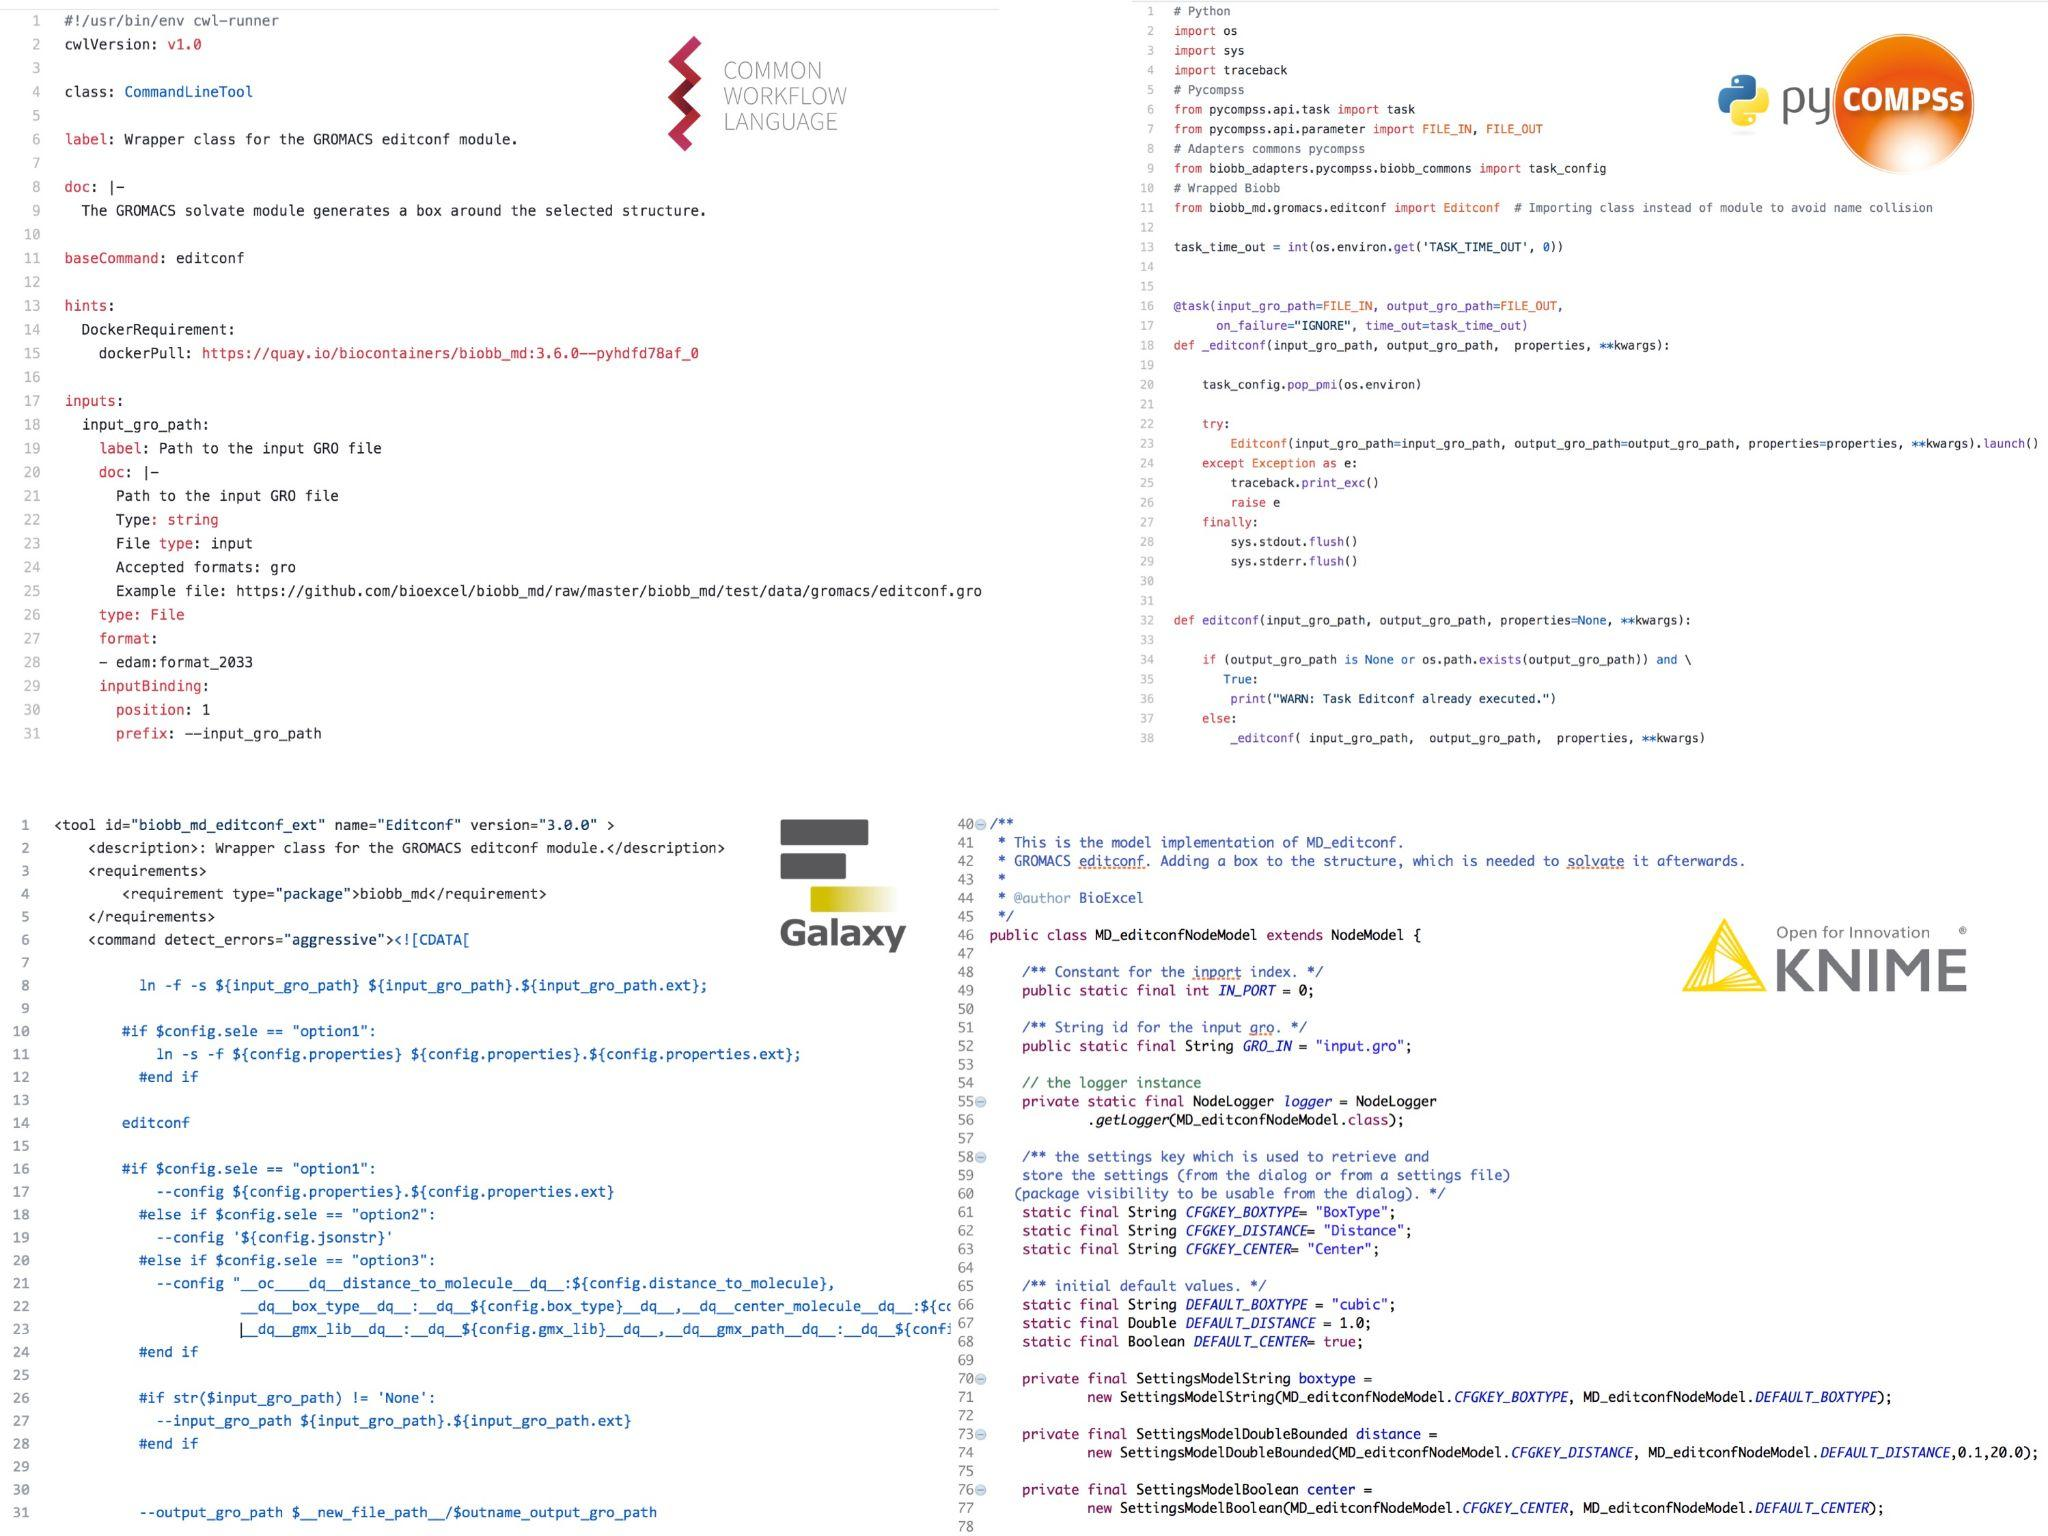
\includegraphics[width=\textwidth]{figures/ch06/figure1.jpg}
	\caption[Code snippets for the BioBB
  WfMS bindings]{\textbf{Code snippets for the BioBB
  WfMS bindings}: CWL, PyCOMPSs, Galaxy and KNIME.}
  \label{ch6:figure1}
\end{figure}

The library is showcased through a collection of
\href{http://mmb.irbbarcelona.org/biobb/workflows}{demonstration
workflows} \cite{ch6-12}. Here, each workflow introduces individual building
blocks as needed to explain a particular scientific computational
method. We primarily expose the workflows as Jupyter Notebooks \cite{Kluyver 2016},
which has been highlighted as a valuable tool for reproducible
scientific workflows \cite{ch6-14}. This offers a graphical interactive
interface, including documentation (integrated markdown) related to the
workflow and the building blocks used, but also to the biomolecular
simulation methods used in the pipeline. Moreover, as we have
demonstrated with our own
\href{https://hub-bioexcel-binder.tsi.ebi.ac.uk/}{Binder} \cite{ch6-15}
hosting, these workflows are reproducible across platforms, assisted by
BioConda \cite{Gruning 2018a} packaging of the building blocks and their software
dependencies.

This assembly of available demonstration workflows have been
successfully used in the BioExcel CoE for dissemination with a range of
\href{https://mmb.irbbarcelona.org/biobb/about/training}{training
events} (e.g.~BioExcel Summer \& Winter School, webinars and virtual
training). In training we particularly utilised the Binder
infrastructure of the BioExcel Cloud portal \cite{ch6-17} to give users a
web-based first experience of the building blocks before they try them
in other workflow systems.

We can observe that workflow building blocks such as BioBB are
necessarily composed of a comprehensive list of digital objects,
encompassing source code, packaging, containerization, documentation,
attributions, citations, registry entries, WfMS integrations and REST
APIs.

We propose to consider building blocks as \emph{composite digital
objects} in their own right: gathering the above software components
along with their metadata, identifiers and operations then forms a
\emph{Canonical Workflow Building Block} (\textbf{CWBB}). We suggest
this concept as a fundamental element of FAIR Digital Objects for
Computational Workflows: researchers use the building blocks
computationally as functional operations across WfMSs, while the FAIR
aspect of CWBB propagates information and resources that are essential
for reproducibility, reuse and understanding by anyone discovering the
workflow.

\subsubsection{Interoperability across different workflow
languages}\label{interoperability-across-different-workflow-languages}

The concept of Canonical Workflow Building Blocks is here showcased with
the BioBB library, by using a transversal workflow present in many
different computational biomolecular projects: a
\href{http://mmb.irbbarcelona.org/biobb/workflows/tutorials/md_setup}{Molecular
Dynamics (MD) protein setup}. This workflow prepares a protein structure
to be used as input for an MD simulation, going through a series of
steps where the protein is completed (adding hydrogen and missing
atoms), optionally introducing a residue mutation, then submerging the
protein in a virtual box of water molecules with a particular ionic
concentration, and finally energetically equilibrating the system (so
that solvent and ions are well accommodated around the protein at the
desired temperature).

This simulation process involves a non-negligible number of steps, using
a variety of biomolecular tools. The BioBB library was used to assemble
this workflow, interconnecting building blocks using Python functions
(Jupyter Notebook, Command Line Interface), auto-generated bindings
(Galaxy \cite{Afgan 2018}, CWL \cite{Crusoe 2022}, PyCOMPSs \cite{ch6-20}) or manually generated
bindings (KNIME \cite{ch6-21}). Corresponding workflows for the different
WfMS can be found in
\href{https://workflowhub.eu/collections/3}{WorkflowHub} \cite{ch6-22,ch6-23,ch6-24,ch6-25,ch6-26}
and graphical extracts can be seen in Figure \vref{ch6:figure2}.

This example demonstrates how the same canonical building blocks can be
used in different WfMS. Wrappers and tools executed behind the workflows
are exactly the same, but the workflows are built using different WfMS,
some of them in a graphical way (drag \& drop, Galaxy, KNIME), some in a
command line way (Jupyter Notebook, PyCOMPSs, CWL); workflows can be
focused on short/interactive executions (Jupyter Notebook), or on High
Throughput/High Performance Computing (HT-HPC) executions (PyCOMPSs);
some of them prepared for a particular WfMS installation (Galaxy),
others completely system-agnostic (CWL).

The current number of available WfMS bindings include Jupyter Notebook,
PyCOMPSs, CWL, Galaxy and KNIME WfMS, in addition to a
\href{http://mmb.irbbarcelona.org/biobb/availability/tutorials/command-line}{command
line} mechanism. Thanks to the extensive documentation added in the
source code as Python docstrings, new bindings for available WfMS can be
generated. We are also experimenting with generating a REST API exposing
the building services as Web services. However, it should be noted that
such automatic generation of bindings is not always practically
feasible. As an example, KNIME nodes require a complete Java skeleton
code, as well as a definition of new data types for all inputs/outputs
required, which makes their automatic generation a heavy and potentially
error-prone task. Bindings for workflow languages with a
\emph{domain-specific language} (DSL) for tool definitions (e.g.~Galaxy,
CWL) can on the other hand be generated in a more straightforward
fashion.

\begin{figure}%[t]
  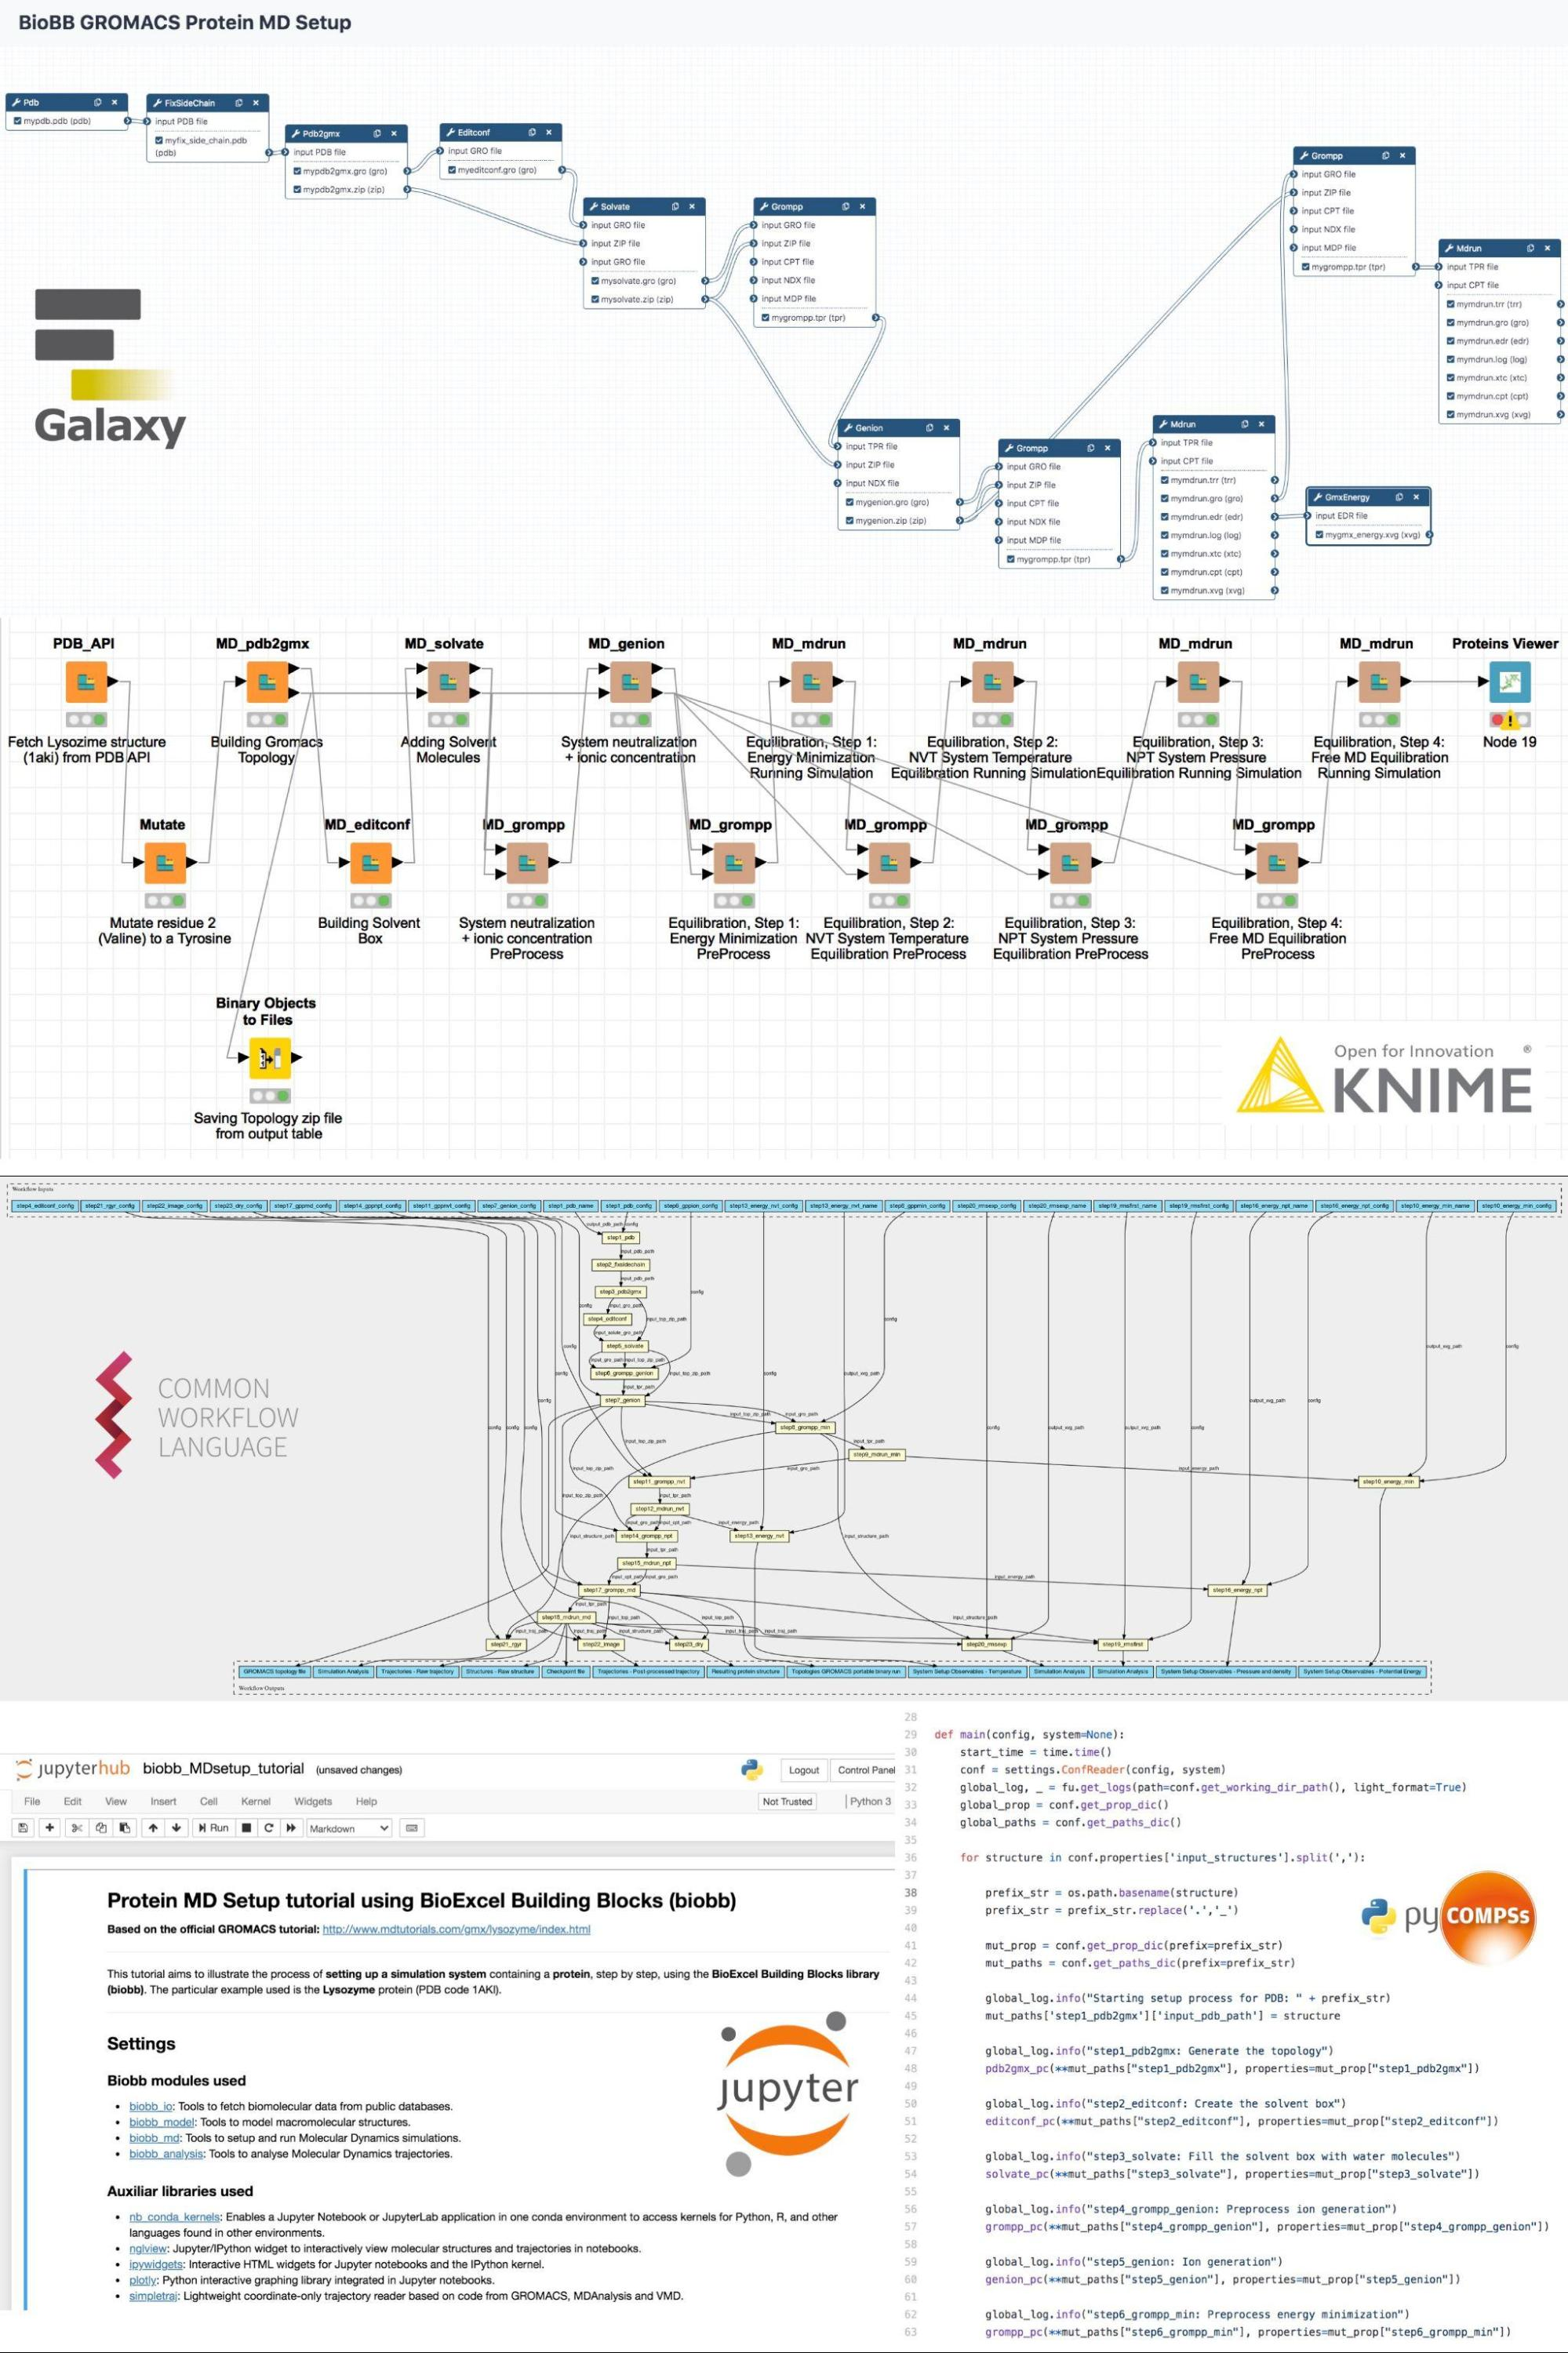
\includegraphics[width=\textwidth]{figures/ch06/figure2.png}
	\caption[Protein MD Setup transversal workflow]{\textbf{Protein MD Setup
  transversal workflow}. Assembled in with 5 different workflow
  managers using BioBB canonical building blocks. From top-left: Galaxy
  \cite{ch6-22}, KNIME \cite{ch6-23}, CWL \cite{ch6-24}, Jupyter Notebook \cite{ch6-25},
  PyCOMPSs \cite{ch6-26}.}
  \label{ch6:figure2}
\end{figure}

The transversal \href{https://workflowhub.eu/collections/3}{protein MD
setup workflow} was chosen as a real example that is readily
understandable by domain experts. More
\href{https://mmb.irbbarcelona.org/biobb/workflows}{complex pipelines}
involving a broader set of wrapped biomolecular tools have been
developed using the BioBB library, primarily as Jupyter Notebooks. A
selection of these have similarly been assembled for different WfMS
using the auto-generated bindings and uploaded to the
\href{https://workflowhub.eu/projects/11\#workflows}{WorkflowHub
repository}.

\subsection{Discussion}\label{discussion-1}

Early work on libraries of workflows fragments include Web Service-based
approaches where tools are wrapped and exposed using common,
interoperable data types in \href{http://biomoby.open-bio.org/}{BioMoby}
\cite{ch6-27} for bioinformatics and similarly
\href{https://en.wikipedia.org/wiki/CaBIG}{caBIG} \cite{ch6-28} for cancer
genomics. While these efforts were interoperable across WfMSs they
required a large up-front investment in agreeing to and adapting native
data to common RDF or XML representations.

The notion of \emph{abstract workflows} \cite{ch6-29}, structural workflow
descriptions separated from their concrete execution realisations and
augmented with Linked Data annotations, have been emphasised as
essential for reuse and consistency across workflow systems. Identifying
\emph{common motifs} for workflow operations \cite{ch6-30} (e.g.~Data
preparation, Format transformation, Filter, Combine) are important to
simplify and understand otherwise fine-grained workflow provenance
traces.

Most other efforts to standardise a set of disparate analytical tools
have been done within the scope of a single WfMS, allowing customised
user interaction, data visualisation, configuration and findability, for
instance
\href{http://www.taverna.org.uk/documentation/taverna-2-x/components/}{Taverna
components} had prototypical building blocks \cite{ch6-31} which were
instantiated at runtime by reference from a registry.
\href{https://docs.knime.com/2020-07/analytics_platform_components_guide/index.html}{KNIME
components and metanodes}, shared on the
\href{https://hub.knime.com/}{KNIME Hub} are frequently designed to be
interoperable, but with a perhaps weaker notion of component families.
The \href{https://toolshed.g2.bx.psu.edu/}{Galaxy toolshed} \cite{ch6-32} is
likewise populated with different sets of tool wrappers that are largely
made to be interoperable within a category.

The \emph{Common Workflow Language} (\textbf{CWL}) \cite{Crusoe 2022} has a strong
emphasis on interoperable command line tool descriptions, with
\href{https://www.commonwl.org/user_guide/07-containers/}{support for
containers} and Conda packaging, as well as
\href{https://www.commonwl.org/user_guide/17-metadata/}{support for FAIR
metadata} like contributors, license and EDAM ontology type annotations.
With multiple leading workflow engines now supporting CWL, and
experimental Galaxy support, this seems perhaps the most promising
candidate for both making and describing canonical workflow building
blocks, however we've identified a few stumbling blocks.

One obvious challenge is that the implementing WfMS needs to have CWL
support, along with support for either containers or Conda packaging to
find the described executables. While it is possible to run a CWL tool
directly using a \texttt{\#!/usr/bin/env\ cwl-runner}
\href{https://en.wikipedia.org/wiki/Shebang_(Unix)}{shebang} on POSIX
systems, this still requires pre-installation and possibly configuration
of a CWL engine like \href{https://pypi.org/project/cwltool/}{cwltool}
or \href{https://toil.readthedocs.io/en/latest/running/cwl.html}{Toil}
\cite{ch6-33}. However workflow engines have multiple dependencies and often
cannot easily be run from a container themselves\footnote{To execute the
  wrapped tool, a containerized workflow engine would need \emph{nested
  containers} which are not generally recommended for security reasons.
  It is possible to work around this limitation using
  \href{https://sylabs.io/singularity/}{Singularity} or
  \href{https://docs.bioexcel.eu/cwl-best-practice-guide/devpractice/containers/conda.html}{Conda}.}.

Within the CWL community it was originally envisioned that a wider set
of workflow systems would adopt CWL for tool description/execution, with
a subset implementing full CWL workflow support. This would allow shared
community effort for describing tools, say in the
\href{https://github.com/common-workflow-library/}{Common Workflow
Library}, rather than each WfMS needing to duplicate this tool wrapping
in separate repositories and languages. However, with the exception of
experimental tool support in Galaxy, in practice all CWL implementers
have gone for full workflow support.

Another challenge is that making a set of building blocks frequently
requires the use of \emph{shims}, for instance file conversion, small
search/replace operations or file renames. In a CWL approach these can
either be performed with an
\href{https://www.commonwl.org/v1.2/Workflow.html\#Expressions_(Optional)}{Expression}
using JavaScript snippets which only has limited access to file content,
or as an additional workflow step added before or after the main tool
step. This combination could then be nested as a subworkflow, similar to
KNIME's \emph{metanodes}, and would also be flexible by allowing
different containers or packages for any pre- or post-steps. Such a CWL
building block however becomes harder to access from a non-CWL WfMS,
because of lack of control over configuration/execution options for the
now nested CWL tools. In practice\footnote{It is worth mentioning that
  it would also be possible to generate WfMS-specific bindings from CWL
  descriptions (e.g.~as demonstrated with
  \href{https://github.com/common-workflow-lab/cwl2script}{cwl2script}
  for Bash,
  \href{https://github.com/common-workflow-lab/gxargparse}{gxargparse}
  for Galaxy,
  \href{https://github.com/common-workflow-lab/cwl2wdl}{cwl2wdl} for
  WDL), although this necessitates constraining the tool and workflow
  definitions to a limited mappable subset of CWL.}, executing a nested
CWL workflow from a native WfMS language would require the engine to
implement full CWL Workflow support (or delegate to a CWL engine).

For the main BioBB building blocks we implemented
\href{http://mmb.irbbarcelona.org/biobb/workflows}{demonstrator
workflows} that highlight how the tools should be used in different
workflow management systems; each having a primary exemplar using
Jupyter Notebook, which can be explored interactively using the
\href{https://hub-bioexcel-binder.tsi.ebi.ac.uk/h}{BioExcel Binder}. If
we consider the abstract demonstrator workflows as \emph{canonical
workflows} they are therefore very much active objects, but can also be
seen as \emph{workflow templates}, as any real use case will need to
specialise the workflow to tweak parameters, data selection etc.

We therefore also provide such workflow templates for multiple WfMS,
including CWL, PyCOMPSs and Galaxy. These are fairly disparate workflow
languages, yet by the use of the same canonical workflow building blocks
(which again invoke the same software binaries), such WfMS-specific
workflows effectively are instantiations of the same canonical workflow.

One challenge found is how to publish such canonical workflows in
registries like the \href{https://workflowhub.eu/}{WorkflowHub}. The hub
supports the registration of Digital Objects in the form of RO-Crate
\cite{Soiland-Reyes 2022}, with the option of abstract CWL for describing the canonical
workflow template, along with direct references to the workflow's GitHub
repository.

For instance in the RO-Crate for
\url{https://doi.org/10.48546/workflowhub.workflow.200.1} \cite{ch6-26},
which can also be
\href{https://rawcdn.githack.com/bioexcel/biobb_hpc_workflows/53958e7c278e53c277a7217057b785482f193f7f/ro-crate-preview.html}{rendered}
from GitHub, we have an entry for the
\emph{\href{https://rawcdn.githack.com/bioexcel/biobb_hpc_workflows/53958e7c278e53c277a7217057b785482f193f7f/ro-crate-preview.html\#workflows/MD/md_list.py}{main
workflow}} according to the
\href{https://w3id.org/workflowhub/workflow-ro-crate/1.0}{Workflow
RO-Crate profile}, detailing each canonical workflow building block used
(e.g.~\href{https://rawcdn.githack.com/bioexcel/biobb_hpc_workflows/53958e7c278e53c277a7217057b785482f193f7f/ro-crate-preview.html\#https\%3A//pypi.org/project/biobb-md/3.6.0/}{biobb-md
metadata}). Here the FAIR aspect of the building blocks to help software
citation is exercised, as the building block wrapper has one set of
authors, documentation and licence (Apache-2.0), while the wrapped
software
(e.g.~\href{https://rawcdn.githack.com/bioexcel/biobb_hpc_workflows/53958e7c278e53c277a7217057b785482f193f7f/ro-crate-preview.html\#https\%3A//doi.org/10.5281/zenodo.2564764}{GROMACS
metadata}) has different authors, licence (GPL-2.1+) and documentation.

However, the deposit of such RO-Crates in WorkflowHub results in one
registration entry per workflow language, which are not otherwise
related and may not even share the same source code repository. Thus,
we've identified the need for adding an overall \emph{canonical workflow
entry}, which can bring in workflow documentation and references shared
across WfMS implementations, including a set of links to the more
granular canonical workflow building blocks used by the workflow, but
also to the individual WfMS implementations as separate digital objects.

A similar question of granularity applies at the workflow tool level
\cite{ch6-4}, particularly for Findability and Accessibility, as we can
consider at lowest granularity the \emph{scientific method} in general
(e.g.~any algorithm for sequence alignment), followed by an
\emph{application suite} (bio.tools entry \cite{ch6-35}, homepage,
documentation), instantiated as a particular \emph{software
installation} (Debian package, Docker container) with its dependencies
at same level. The installation includes one or more \emph{software
executables} (a particular binary, a running service service), providing
at the highest detailed granularity level the specific types of
\emph{software functionality} (a particular mode of operation, choice of
analysis), for instance using certain command line flags.

For canonical workflow building blocks, with a focus on pluggable
composability, this is mainly defined at this high granularity level of
specific software functionality: explicit operations from an installed
tool, which are then combined in a workflow. This is indeed the level
WfMS tool definitions are typically done, e.g.~a CWL Command Line Tool
specifies a particular way to run a particular software binary. However,
to be an actionable CWBB, the building block needs to additionally
convey the lower granularity levels; particularly to support multiple
options for interoperable installation and execution, as well as
metadata at the most general level, such as documentation and scholarly
citations.

While workflow management systems typically only operate at the highest
granularity levels for execution details, and are frequently unaware of
(or not exposing metadata at) the more general levels, we argue that in
order for a Canonical Workflow \cite{cwfr} to follow and support FAIR
principles for itself and its data, the workflow management system need
to \emph{propagate structured metadata} about the tools used by the
workflow. We propose that in order to support the workflow's
applicability to multiple WfMS, the tools themselves must also have a
consistent packaging and formal description that enables consistent
computational invocation.

At the most general level, a canonical workflow built using such CWBBs
is even conceptually reproducible because the FAIR documentation of the
workflow, through its canonical workflow building blocks, identifies how
individual tools and software applications are composed, which in worst
case can be rebuilt using different installation methods in a different
WfMS, or in best case inspected to detect and cross-link the same
canonical workflow appearing in different WfMS instantiations. This view
of software as composition of other software typically also applies at
individual tool level, which themselves depend on programming language
runtimes, libraries, services and reference data.

\subsection{Requirements for Canonical Workflow Building
Blocks}\label{requirements-for-canonical-workflow-building-blocks}

Building on the experiences with BioBB, we here propose requirements and
recommendations for establishing Canonical Workflow Building Blocks
(CWBB) as implementations of \emph{canonical steps} introduced for
Canonical Workflow Frameworks for Research \cite{cwfr}.

The core purpose of a CWBB is to wrap a command line tool or other
software that can perform an operation as part of a computational
workflow. As such, the general advice for making software workflow-ready
applies \cite{ch6-37} (e.g.~easy to install, documented, parallelizable,
reproducible output), however a CWBB is also permitted to make use of
additional scripts or \emph{shims} to further adapt a third-party tool
for workflow use and for data interoperability across blocks.

The way tools are installed or invoked varies slightly across WfMS and
operating systems, therefore a CWBB should provide multiple methods for
distributing software; currently containers (Docker, Singularity) and
distribution-independent packaging (e.g.~Conda, Homebrew) are promising
by having reproducible install recipes and a wide range of open source
dependencies (e.g.~Java, Python). Additionally building blocks should
allow overriding execution paths, e.g.~for use with HPC module system
and hardware-optimised binaries.

The CWBBs should have sufficient annotations to be able to generate
bindings for different WfMSs and REST APIs, e.g.~parameter names and
descriptions, types and default values; enumerators for options, file
formats for inputs/outputs.

Building blocks should be grouped into families that are interoperable
through common data structures and file formats, as well as having joint
naming conventions for configuration options. A CWBB family should be
released as a single version following
\href{https://semver.org/spec/v2.0.0.html}{semantic versioning} rules,
which should have a corresponding persistent identifier (PID) \cite{McMurry 2017}.

Metadata for CWBBs should be captured following FAIR guidelines, and
distributed as part of the block family and resolvable from the PID as a
FAIR Digital Object. Metadata should include references to the CWBB
software distributions (e.g.~\href{https://quay.io/search}{quay.io}
container URL) as well as attributions, citations and documentation for
the wrapped tool.

Example workflows showing CWBB usage should be included in a
WfMS-neutral language such as Jupyter Notebooks, which may have
equivalent variants for each workflow binding. These workflows should be
registered in a workflow registry like WorkflowHub or Dockstore, and
assigned their own PIDs.

\subsection{Conclusions}\label{conclusions}

The proposed concept of Canonical Workflow Building Blocks can bridge
the gap between FAIR Computational Workflows, interoperable
reproducibility and for building canonical workflow descriptions to be
used and described FAIRly across WfMSs.

The realisation of CWBBs can be achieved in many ways, not necessarily
using the Python programming language together with RO-Crate as explored
here. In particular if the envisioned Canonical Workflow Frameworks for
Research become established in multiple WfMSs with the use of FAIR
Digital Objects, the different implementations will need to agree on
object types, software packaging and metadata formats in order to reuse
tools and provide interoperable reproducibility for canonical workflows.

Likewise, to build a meaningful collection of building blocks for a
given research domain, a directed collaborative effort is needed to
consistently wrap tools for a related set of WfMSs, chosen to target
particular use cases (a family of canonical workflows).

For individual users, a library of Canonical Workflow Building Blocks
simplifies many aspects of building pipelines, beyond the FAIR aspects
and data compatibility across blocks. For instance, they can benefit
from training of a CWBB family using Jupyter Notebooks, and then use
this knowledge to utilise the same building blocks in a scalable HPC
workflow with a CWL engine like Toil, knowing they will perform
consistently thanks to the use of containers.

While we have demonstrated CWBB in the biomedical domain, this approach
is generally applicable to a wide range of sciences that execute
pipelines of multiple file-based command line tools, however it may be
harder to achieve with more algebraic ``in memory'' types of
computational workflows, where steps could be challenging to
containerize and distinguish as separate block.

We admit that biomolecular research is quite a homogenous field with
respect to computational analyses and now becoming relatively mature in
terms of tool composability in workflows, building on the experiences of
the ``FAIR pioneers'' in the field of bioinformatics. Other fields, such
as social sciences or ecology, can have a wider variety of methods and
computational tools, often with human interactions, and may have to
adapt the software to be workflow-ready \cite{ch6-37} before using them as
Canonical Workflow Building Blocks. Domains adapting CWBB approach (or
workflow systems in general) should take note of the great benefits of
hosting collaborative events where developers meet each other and their
potential users, demonstrated in our field with events such WorkflowsRI
\cite{ch6-39} and Biohackathons \cite{ch6-40}.

The Common Workflow Language shows promise as a general canonical
workflow building blocks mechanism: gathering execution details of tools
along with their metadata and references, augmented with
\href{https://docs.bioexcel.eu/cwl-best-practice-guide/devpractice/partial.html\#using-abstract-operations-as-placeholders}{abstract
workflows} to represent canonical workflows. However, this would need
further work to implement our CWBB recommendations in full. Future work
for the Canonical Workflow Building Blocks concept includes formalising
and automating publication practises, to make individual blocks
available as FAIR Digital Objects on their own or as part of an
aggregate collection like RO-Crate.

\section{Incrementally building FAIR Digital Objects with Specimen Data
Refinery
workflows}
\label{ch7:incrementally-building-fair-digital-objects-with-specimen-data-refinery-workflows}

\emph{Specimen Data Refinery} (SDR) is a developing platform for
automating transcription of specimens from natural history collections
\cite{Hardisty 2022} (section \vref{ch8:the-specimen-data-refinery}). SDR is
based on computational workflows and digital twins using FAIR Digital
Objects.

We show our recent experiences with building SDR using the Galaxy
workflow system and combining two FDO methodologies with open digital
specimens (openDS) and RO-Crate data packaging. We suggest FDO
improvements for incremental building of digital objects in
computational workflows.

\subsection{SDR workflows}\label{ch7:sdr-workflows}

SDR\footnote\url{https://sdr.nhm.ac.uk/} is realised as the workflow system
Galaxy \cite{Afgan 2018} with
SDR tools\footnote\url{https://github.com/DiSSCo/SDR} installed. An Open
Research challenge is that some tools have machine learning models with
a commercial licence. This complicates publishing to
Galaxy toolshed\footnote\url{https://toolshed.g2.bx.psu.edu/}, however we
created Ansible\footnote{\url{https://www.ansible.com/}} scripts to install
equivalent Galaxy servers, including tools and dependencies, accounts
and workflows. SDR workflows are
published\footnote\url{https://workflowhub.eu/projects/72} in WorkflowHub as
FDOs.

We implemented the use case \emph{De novo digitization} in Galaxy \cite{Brack 2022}.
Shown in Figure \vref{ch7:figure1} the
workflow steps exchange openDS JSON \cite{Hardisty 2019}, for
incremental completion of a digital specimen. Initial stages build a
template openDS from a CSV with metadata and image references --
subsequent analysis completes the rest of the JSON with \emph{regions}
of interest, \emph{text} digitised from handwriting, and recognized
\emph{named entities}.

\begin{figure}%[t]
    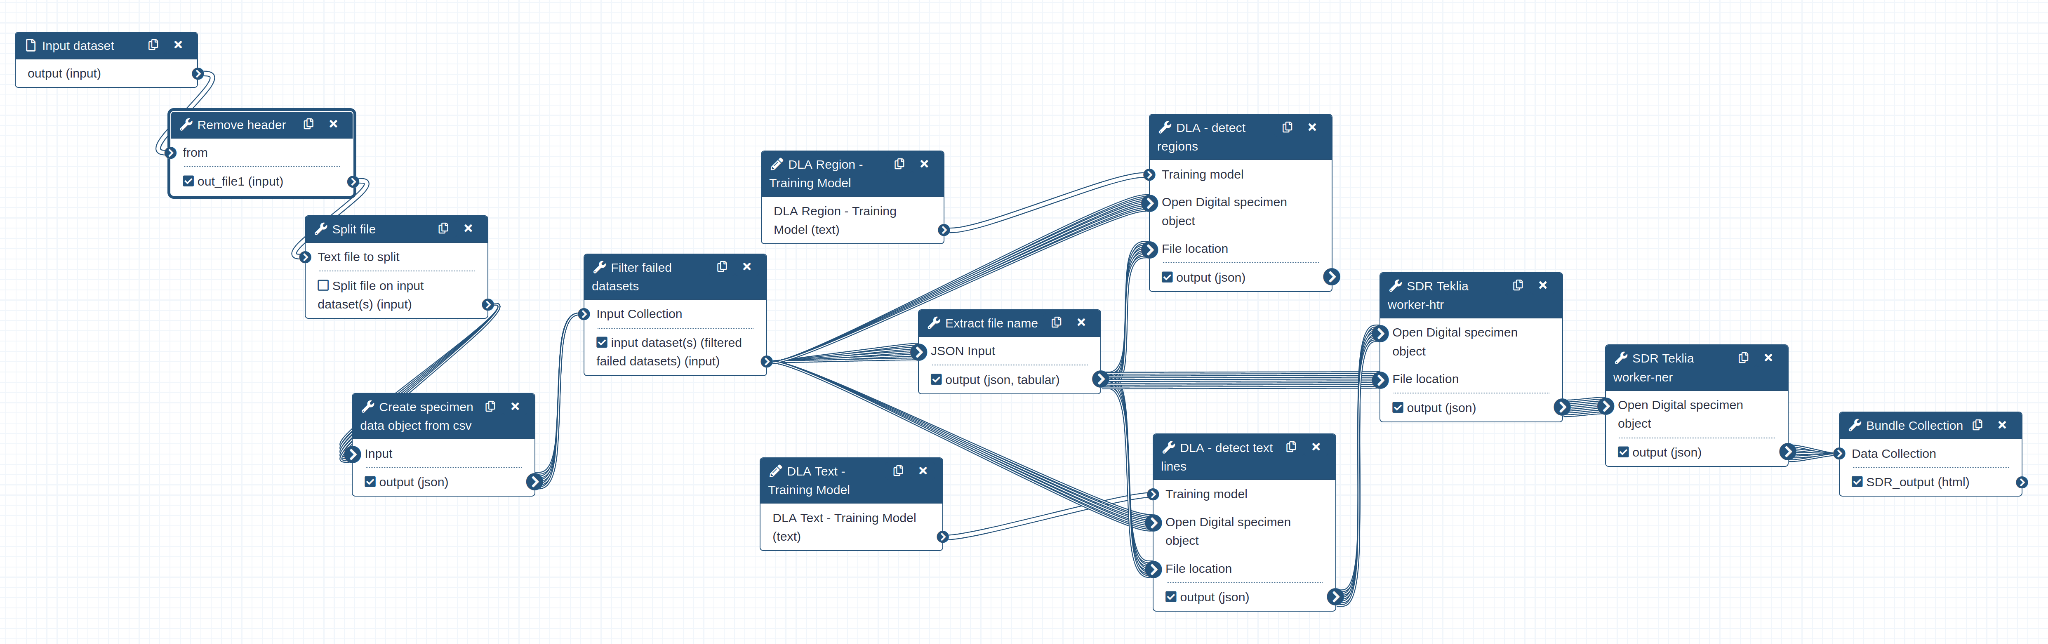
\includegraphics[width=\textwidth]{figures/ch07/figure1.png}
	\caption[FDO propagation in workflow]{\textbf{FDO propagation in workflow}. 
    Draft Galaxy workflow \cite{Brack 2022} 
    shows propagation of partial Open Digital Specimen FDOs between
    individual canonical workflow building blocks. First steps process a CSV
    file to create the initial openDS, where referenced images are analysed
    to detect text lines which are OCRed and then recognized as named
    entities. Bands indicate flow of collections of openDS, processed
    concurrently by each step. The final step bundles the collection of
    openDS FDOs as JSON files in a ZIP archive.}
    \label{ch7:figure1}
  \end{figure}

Galaxy can visualise outputs of each step
(Figure \vref{ch7:figure2}), important to make the
FDOs understandable by domain experts and to verify accuracy of SDR.

\begin{figure}%[t]
    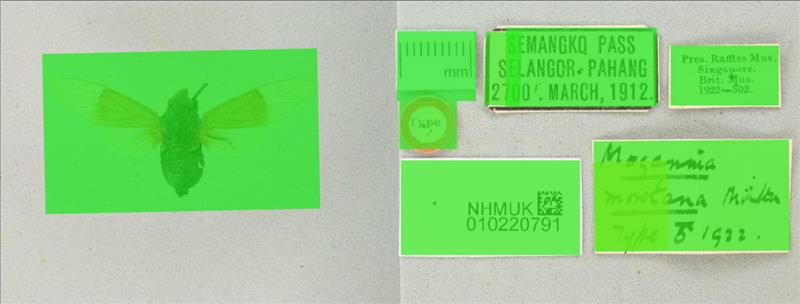
\includegraphics[width=\textwidth]{figures/ch07/figure2.jpg}
	\caption[Visualising openDS FDO within Galaxy]{\textbf{Visualising openDS FDO within Galaxy}.
    Showing detected regions of interest
    (specimen, labels and scale bar) for a pinned insect.}
    \label{ch7:figure2}
\end{figure}

We are adding workflows for partial stages, e.g.~detection of regions
\cite{Livermore 2022a} and hand-written text recognition
\cite{Livermore 2022b}, which we'll combine with scalability testing and wider
testing by project users. Additional workflows will enhance existing
FDOs and use new tools such as barcode detection of museums' internal
identifiers.

We are now ready to publish digital specimens as FAIR Digital Objects,
with registration into DiSSCO repositories\footnote\url{https://www.dissco.eu/dissco/technical-infrastructure/}, PID assignment and workflow provenance. However, even at
this early stage we have identified several challenges that need to be
addressed.

\subsection{FDO lessons}\label{ch7:fdo-lessons}

We highlight the \emph{De novo} use case because this workflow is
exchanging \emph{partial} FDOs -- openDS objects which are not fully
completed and not yet assigned persistent identifiers.
openDS schemas\footnote\url{https://github.com/DiSSCo/openDS} are still in
development, therefore SDR uses a
more flexible
JSON schema\footnote\url{https://github.com/DiSSCo/SDR/blob/main/galaxy-workflow/config/opends-schema.json} where only the initial metadata (populated from CSV) are
required. Each step validates the partial FDO before passing it to the
underlying command line tool.

Although workflow steps exchange openDS objects, they cannot be combined
in any order. For instance, \emph{named entity recognition} requires
digitised text in the FDO. We can consider these intermediate steps as
\emph{sub-profiles} of an FDO Type. Unlike hierarchical subclasses,
these FDO profiles are more like
\href{https://en.wikipedia.org/wiki/Duck_typing}{ducktyping}. For
instance a \emph{text detection} step may only require the
\texttt{regions} key, but semantically there is no requirement for say
\texttt{OpenDSWithText} to be a subclass of \texttt{OpenDSWithRegion},
as text also can be transcribed manually without regions.

Similarly, we found that some steps can be executed in parallel, but
this requires merging of partial FDOs. This can be achieved by combining
JSON queries and JSON Schemas, but indicates that it may be more
beneficial to have FDO fragments as separate objects. Adding openDS
fragment steps would however complicate workflows.

Several of our tools process the referenced images, currently https URLs
in openDS. We added a caching layer to avoid repeated image downloading,
coupled with local file-paths wiring in the workflow. A similar
challenge occurs if accessing image data using DOIP, which unlike HTTP,
has no caching mechanisms.

\subsection{RO-Crate lessons}\label{ch7:ro-crate-lessons}

Galaxy is developing support for importing and
exporting Workflow
Run Crates\footnote\url{https://www.researchobject.org/workflow-run-crate/}, a profile of RO-Crate \cite{Soiland-Reyes 2022} to
captures execution history of a workflow, including its definition and
intermediate data \cite{De Geest 2022}. SDR is adopting this support to
combine openDS FDOs with workflow provenance, as envisioned by
\cite{Walton 2020}.

Our prototype \emph{de novo} workflow returns results as a ZIP file of
openDS objects. End-users should also get copies of the referenced
images and generated visualisations, along with workflow execution
metadata. We are investigating ways to embed the preliminary Galaxy
workflow history before the final step, so that this result can be an
enriched RO-Crate.

\subsection{Conclusions}\label{ch7:conclusions}

SDR is an example of machine-assisted construction of FDOs, which
highlight the needs for intermediate digital objects that are not yet
FDO compliant. The passing of such ``local FDOs'' is beneficial not just
for efficiency and visual inspection, but also to simplify workflow
composition of canonical workflow building blocks. At the same time we
see that it is insufficient to only pass FDOs as JSON objects, as they
also have references to other data such as images, which should not need
to be re-downloaded.

Further work will investigate the use of RO-Crate as a wrapper of
partial FDOs, but this needs to be coupled with more flexible FDO types
as profiles, in order to restrict ``impossible'' ordering of steps
depending on particular inner FDO fragments. A distinction needs to be
made between open digital specimens that are in ``draft'' state and
those that can be pushed to DiSSCo registries.

We are experimenting with changing the SDR components into Canonical
Workflow Building Blocks \cite{Soiland-Reyes 2022a}
(\vref{ch6:making-canonical-workflow-building-blocks-interoperable-across-workflow-languages}) 
using the Common Workflow Language \cite{Crusoe 2022}. This gives
flexibility to scalably execute SDR workflows on different compute
backends such as HPC or local cluster, without the additional setup of
Galaxy servers.


\section{The Specimen Data Refinery}
\label{the-specimen-data-refinery}

\subsection*{A canonical workflow framework and FAIR Digital Object
approach to speeding up digital mobilisation of natural history
collections}

A key limiting factor in organising and using information from physical
specimens curated in natural science collections is making that
information computable, with institutional digitization tending to focus
more on imaging the specimens themselves than on efficiently capturing
computable data about them. Label data are traditionally manually
transcribed today with high cost and low throughput, rendering such a
task constrained for many collection-holding institutions at current
funding levels.

We show how computer vision, optical character recognition, handwriting
recognition, named entity recognition and language translation
technologies can be implemented into canonical workflow component
libraries with findable, accessible, interoperable, and reusable (FAIR)
characteristics. These libraries are being developed in a cloud-based
workflow platform -- the `Specimen Data Refinery' (SDR) -- founded on
Galaxy workflow engine, Common Workflow Language, Research Object Crates
(RO-Crate) and WorkflowHub technologies. The SDR can be applied to
specimens' labels and other artefacts, offering the prospect of greatly
accelerated and more accurate data capture in computable form.

Two kinds of FAIR Digital Objects (FDO) are created by packaging outputs
of SDR workflows and workflow components as digital objects with
metadata, a persistent identifier, and a specific type definition. The
first kind of FDO are computable Digital Specimen (DS) objects that can
be consumed/produced by workflows, and other applications. A single DS
is the input data structure submitted to a workflow that is modified by
each workflow component in turn to produce a refined DS at the end. The
Specimen Data Refinery provides a library of such components that can be
used individually, or in series. To cofunction, each library component
describes the fields it requires from the DS and the fields it will in
turn populate or enrich. The second kind of FDO, RO-Crates gather and
archive the diverse set of digital and real-world resources,
configurations, and actions (the provenance) contributing to a unit of
research work, allowing that work to be faithfully recorded and
reproduced.

Here we describe the Specimen Data Refinery with its motivating
requirements, focusing on what is essential in the creation of canonical
workflow component libraries and its conformance with the requirements
of an emerging FDO Core Specification being developed by the FDO Forum.

\hypertarget{introduction-2}{%
\subsection{Introduction}\label{introduction-2}}

A key limiting factor in organising and using information from physical
specimens curated in natural history collections is making that
information computable (`machine-actionable') and extendable. More than
85\% of available information currently resides on labels attached to
specimens or in physical ledgers \cite{ch8-1}. Label data are commonly
transcribed manually with high cost and low throughput, rendering such a
task constraining for many institutions at current funding levels.
However, the advent of rapid, high-quality digital imaging has meant
that digitizing specimens, including their labels, is now faster and
cheaper \cite{ch8-2}. With initiatives such as Advancing Digitization of
Biological Collections (ADBC), integrated Digitized Biocollections
(iDigBio) and the Distributed System of Scientific Collections (DiSSCo)
\cite{ch8-3,ch8-4,ch8-5,ch8-6} aiming to increase the rate and accuracy of both mass and
on-demand digitization of natural history collections, the gap between
expectations of what should be digitally available and computable, and
what can be achieved using traditional transcription approaches is
widening. Modern, highly efficient workflow tools and approaches can
play a role to address this.

Collection digitization began towards the end of the 20th century by
typing basic data from labels into the collection (asset) management
systems of collection-holding institutions such as natural history
museums, herbaria and universities. Initially, this was to facilitate
indexing and cataloguing and locating the physical specimens, but with
the addition of photographic images of specimens and the public
availability of specimen data records, through data portals of the
institutions themselves as well as international data infrastructures
like the Global Biodiversity Information Facility (GBIF), such bodies of
data have been rapidly exploited for research \cite{ch8-7,ch8-8}. It has become
clear that widespread digitization of data about physical specimens in
collections and the advent of high-throughput digitization processes
\cite{ch8-9,ch8-10,ch8-11,ch8-12,ch8-13} is transforming and will radically further transform the
range of scientific research opportunities and questions that can be
addressed \cite{ch8-14,ch8-15}. Scientific conclusions and policy decisions
evidenced by digital specimen data enhance humankind's ability to
conserve, protect, and predict the biodiversity of our world
\cite{ch8-16,ch8-17}.

Harnessing technologies developed to harvest, organise, analyse and
enhance information from sources such as scholarly literature,
third-party databases, data aggregators, data linkage services and
geocoders and reapplying these approaches to specimens' labels and other
artefacts offers the prospect of greatly accelerated data capture in a
computable form \cite{ch8-18}. Tools of particular interest span the fields
of computer vision, optical character recognition, handwriting
recognition, named entity recognition and language translation.

Workflow technologies from the ELIXIR Research Infrastructure \cite{ch8-19},
including Galaxy \cite{ch8-20}, Common Workflow Language \cite{ch8-21}, Research
Object Crates (RO-Crates) \cite{OCarragain 2019,ch8-23} and WorkflowHub \cite{ch8-24}, and
selected tools are integrated in a cloud-based workflow platform for
natural history specimens -- the `Specimen Data Refinery' \cite{ch8-1} that
will become one of the main services to be offered by the planned DiSSCo
research infrastructure \cite{ch8-25}. The tools themselves, implemented with
findable, accessible, interoperable, and reusable (FAIR) characteristics
\cite{ch8-26} are packaged into canonical workflow component libraries
\cite{ch8-27}, rendering them reusable, and interoperable with one another.
FAIR Digital Objects are adopted as the common input/output pattern,
fully compatible with digital objects at the core of DiSSCo data
management \cite{ch8-28}.

The Refinery brings together domain-specific workflows for processing
specimen images and extracting text and data from images with canonical
forms for components and interactions between components that can lead
to improved FAIR characteristics for both the workflows themselves and
the data resulting from workflow execution.

FAIR Digital Objects (FDO) are created by packaging outputs of workflows
and workflow components as digital objects with metadata, a persistent
identifier, and a specific type definition against which operations can
be executed \cite{ch8-29}. The Refinery uses two kinds of FDOs:

\begin{itemize}
\item
  \textbf{computable Digital Specimen (DS) objects} \cite{ch8-30} from DISSCo
  for the scientific input/output data that can be consumed/produced by
  workflows and other applications.
\item
  \textbf{workflow objects, implemented as RO-Crates} \cite{ch8-23}, from
  ELIXIR gather and archive the diverse set of workflow process data --
  the digital and real-world resources, configurations and actions (the
  provenance) contributing to a unit of digitization or other work
  producing the Digital Specimen digital objects, allowing that work to
  be scrutinised and faithfully reproduced if necessary.
\end{itemize}

We first summarise related work before describing the problem to be
addressed by the Specimen Data Refinery. We then explain our Canonical
Workflows for Research (CWFR) approach using these FDOs in the design of
the SDR, the experimental setup, and results so far from the work in
progress. While future work will clarify full results and challenges of
implementing a robust, reliable, and easy-to-use production-capability
SDR, in this early report following SDR prototyping and
conceptualization, we focus on what we found to be essential in the use
of FDOs and CWFR canonical step libraries, and on the compliance of
canonical workflow (component) inputs and outputs with the requirements
of the FDO Framework \cite{ch8-31}.

\hypertarget{related-work}{%
\subsection{Related Work}\label{related-work}}

\hypertarget{workflows-for-processing-specimen-images-and-extracting-data}{%
\subsubsection{Workflows for processing specimen images and
extracting
data}\label{workflows-for-processing-specimen-images-and-extracting-data}}

While natural history collections are heterogeneous in size and shape,
often they are mass digitized using standardised workflows \cite{ch8-9,ch8-10,ch8-11,ch8-12,ch8-13}.
In pursuit of higher throughput at lower cost, yet with higher accuracy
and richer metadata, further automation will increasingly rely on
techniques of object detection and segmentation, optical character
recognition (OCR) and semantic processing of labels, and automated
taxonomic identification and visual feature analysis \cite{ch8-1,ch8-18}.

Although there is a great deal of variety among images of different
kinds of collection objects that are digitized (see figure 1) there are
visual similarities between them. Most images contain labels, scale bars
and often, colour charts as well as the specimen itself. This makes them
amenable to improved approaches to object detection \cite{ch8-32} and
segmentation into `regions of interest' \cite{ch8-33} as precursive steps for
multiple kinds of workflows.

\{\{\textless{} figure src=``figure1.png'' link=``figure1.png''
id=``fig:specimens'' width=``100\%'' title=" A range of specimen images"
caption=``From the Natural History Museum, London, demonstrating the
diversity of collection objects, which include handwritten, typed, and
printed labels. (a) Microscope slide
(\href{https://data.nhm.ac.uk/object/c65d9a3c-d8f6-4fac-a418-05c3b697cece}{NHMUK010671647}),
(b) Herbarium specimen
(\href{https://data.nhm.ac.uk/object/be595f07-73c5-4764-a96c-8b377e3d1507}{BM000546829}),
(c) pinned insect
(\href{https://data.nhm.ac.uk/object/745febc7-8222-498a-9969-5f6b12f85ef3}{NHMUK013383979})''
\textgreater\}\}

Segmentation, specifically, can be employed as an early step in a
workflow to send just the relevant region(s) of interest from an image
to later workflow steps. Not only does this decrease data transfer time
and minimise computational overheads but it can also substantially
increase the accuracy of subsequent OCR processing and semantic
recognition steps \cite{ch8-18}.

Much of the data about specimens is stored on their handwritten, typed
or printed labels or in registers/ledgers \cite{ch8-34}. Direct manual
transcription into local databases with manual georeferencing is the
primary method used today to capture this data. Potentially, OCR can
significantly increase transcription speeds whilst reducing cost;
although it sacrifices accuracy and disambiguation that are today
achieved with specialist knowledge provided by humans during the
process. Returning character strings from OCR is useful, but
semantically placing this data in its context as information specific to
natural history specimens and linking that back to the original physical
specimens is of much higher value, improving the utility of natural
history collections. Shortfalls in accuracy and disambiguation can be
made up by exploiting Natural Language Processing (NLP) advances such as
named entity recognition to identify text segments belonging to
predefined categories (for example, species name, collector, locality,
date) \cite{ch8-18}. Nevertheless, this only works well on a small proportion
of captured data in the absence of `human in the loop' input. To better
automate disambiguation of people's names, for example, access to other
contextual `helper' data are needed (e.g., biographical data in
Wikidata) as well as cross-comparison with other data from the specimen,
such as the date of collection and location \cite{ch8-35}.

Automated identification of species from images of living organisms has
achieved impressive levels of accuracy 
\cite{ch8-36,ch8-37,ch8-38,ch8-39,ch8-40,ch8-41} with techniques
translated to an increasing range of enthusiastically received consumer
applications for plant and animal identification using mobile phones
(e.g., \href{https://www.plantsnap.com/}{Plantsnap},
\href{https://www.picturethisai.com/}{PictureThis},
\href{https://www.inaturalist.org/pages/seek_app}{iNaturalist SEEK}).
Automated identification of \emph{preserved specimens}, however,
presents different challenges. Although identification might be made
more accurately because a specimen is presented in a standard manner,
separated from other organisms and the complexity of a natural
background, the loss of colour and distortion of the shape of the
organism arising from preparation and preservation processes can lead to
the loss of important identification clues that might be present on a
living example.

\hypertarget{workflow-management-systems-and-canonical-workflows-for-research}{%
\subsubsection{Workflow management systems and canonical workflows
for
research}\label{workflow-management-systems-and-canonical-workflows-for-research}}

A workflow chains together atomised and executable components with the
relationships between them to clearly define a control flow and a data
flow. Their significant defining characteristics are (i) abstraction,
through the separation of the workflow specification (the work to be
done) from its execution (how it is done), and (ii) composition whereby
the components can be cleanly combined and reused and workflows
themselves can be neatly packaged as components \cite{ch8-42}. Workflow
management systems typically provide the necessary mechanisms for
explicitly defining workflows in a reusable way together with a workflow
engine that executes the workflow steps and keeps an accountable record
of the processing -- logging the codes executed and the data lineage of
the results. In the past decade there has been a rise in popularity in
both the development of WfMS and their use, driven by the increasing
scales of data and the accompanying complexity of its processing
\cite{ch8-42}.

Workflow management systems typically vary in the features they provide
for supporting: workflow programming language and control flow
expressivity; data type management; code wrapping, containerisation and
integration with software management tools; exploitation of
computational architectures; availability of development and logging
tools; licensing and so on. Although several hundred kinds of such
systems exist \cite{ch8-43}, communities tend to cluster around a few popular
systems based on their ``plugged-in'' availability of data type
specialist codes, the catered-for skills level of the workflow
developers, and its documentation, community support and perceived
sustainability. For the Specimen Data Refinery, the Galaxy workflow
system \cite{ch8-20} in conjunction with Common Workflow Language (CWL)
\cite{ch8-21} has been chosen. CWL is a workflow specification standard
geared towards supporting interoperable and scalable production
pipelines, abstracting away from the internal data structures of some of
the language-specific workflow systems.

Originally designed for computational biology and with many available
tool components, Galaxy \cite{ch8-20} supports multiple domains. Workflows
can be built by manually experimenting with data manipulations in a
`data playground' and subsequently converting histories of those to
workflows, or by a more traditional drag-and-drop composition approach.
New components can be created by wrapping existing programs, with
in-built dependency management and automated conversion to executable
containers. As such, Galaxy and CWL offer possibilities for a rich
canonical workflow component landscape with a workflow management regime
that can be both easily FAIR compliant and efficient internally
\cite{ch8-27}. The WorkflowHub, which facilitates CWL and enables workflows
to be registered, shared and published, is mutually coupled with Galaxy
so that workflows can be discovered in the Hub and immediately executed
in a public-use Galaxy instance.

In the context of the SDR, users can construct institution or
project-specific variants of digitization workflows to suit their
specific needs. As collections are heterogeneous, different specimen
types or specific sets of specimens are likely to have variations and
idiosyncrasies in the digitization and processing needed. Tools for
automated identification of specimens are likely to be taxon-specific,
and as such it seems likely that taxon-specific workflows will become
common. In addition, institutions have specific data exchange
requirements for their individual collection management systems.
Ensuring that workflows can be easily modified in a common environment
bridges the gap between community contribution to shared tooling and the
bespoke needs of specific institutions/collections.

Although computational workflows typically emphasize scalable automated
processing, in practice many also combine automation with manual steps.
This feature is also supported by Galaxy and CWL, allowing (for example)
manual geocoding and verification during the digitization process of the
locations where specimens were collected.

\hypertarget{fair-digital-objects-1}{%
\subsubsection{FAIR Digital Objects}\label{fair-digital-objects-1}}

Galaxy/CWL environments offer the possibility to integrate generic
digital object methods \cite{ch8-44,ch8-45,ch8-46} for the interactions between
workflow components, thus making them able to meet the need and ease the
burden of compiling FAIR compliant data throughout the research
lifecycle \cite{ch8-27}.

A digital object exhibiting FAIR characteristics is a FAIR Digital
Object \cite{ch8-29} and is defined formally as ``a unit composed of data
and/or metadata regulated by structures or schemas, and with an assigned
globally unique and persistent identifier (PID), which is findable,
accessible, interoperable and reusable both by humans and computers for
the reliable interpretation and processing of the data represented by
the object''.

Supporting `FAIRness' internally and acting as glue between the steps of
canonical workflows, FDOs record and can represent the state of a
workflow, its inputs and outputs, and the component steps performed in a
comprehensive manner \cite{ch8-27}. Each FDO is anchored by a globally unique
and resolvable, persistent identifier (PID) (such as a DOI®, for
example) that clearly refers to one digital entity. The PID resolution
offers persistent references to find, access and reuse all information
entities that are relevant to access and interpret the content of an
FDO. In doing so, the FDO creates a new kind of machine-actionable,
meaningful and technology independent unit of information. This is both
immediately available and amenable for further use, as well as being
comparable to the role of the classical archival storage box when
necessary.

\hypertarget{computable-digital-specimens-as-a-kind-of-fair-digital-object}{%
\paragraph{Computable Digital Specimens as a kind of FAIR Digital
Object}\label{computable-digital-specimens-as-a-kind-of-fair-digital-object}}

Digital Specimens (DS) are a specific class of FDO that group, manage
and allow processing of fragments of information relating to physical
natural history specimens. On a one-to-one correspondence a DS
authoritatively collates data about a physical specimen (i.e.,
information extracted and captured from labels by digitization
workflows) with other data -- often to be found from third-party sources
-- derived from analysis and use of the specimen.

openDS \cite{ch8-47} is the developing specification for open Digital
Specimens and other related object types, defining: 

\begin{itemize}
  \item The logical
  structure and content of Digital Specimen (DS), Basic Image Object (BIO)
  and other object types, and the operations permitted on them
  \item The
  handling rules and behaviors governing digital specimen object
  operations in general
  \item Serialization and packaging as
  JavaScript Object Notation (JSON) for lightweight data interchange
  between systems, sub-systems and components of systems (for which, read
  `workflow components' \cite{ch8-48}. 
\end{itemize}

openDS is essential to future FAIR
digitization of natural history collections and to Digital Specimens as
self-standing digital objects on the Internet, amenable to computer
processing. It contributes to the new transformative generation of FAIR
infrastructure and applications based on Digital Object Architecture
that is planned for the Distributed System of Scientific Collections
(DiSSCo) \cite{ch8-6,ch8-25,ch8-30} European research infrastructure.

Henceforth we refer to these as openDS FDOs.

\paragraph{FAIR packaging of research/workflow objects with
RO-Crate}\label{fair-packaging-of-researchworkflow-objects-with-ro-crate}

The useful outcomes of research are not just traditional publications
nor data products but everything that goes into and supports an
investigative work or production pipelining activity. This includes
input and intermediate data, parameter settings, final outputs, software
programs and workflows, and configuration information sufficient to make
the work reproducible. Research objects \cite{ch8-49} are a general approach
to describing and associating all of this content together in a
machine-readable form so that it can be easily preserved, shared and
exchanged. Workflow objects are a specific subclass of research objects.

RO-Crate \cite{OCarragain 2019,ch8-23} has been established as a community standard to
practically achieve FAIR packaging of research objects with their
structured metadata. Based on well-established Web standards, RO-Crate
uses JSON-LD \cite{ch8-50} with \href{https://schema.org/}{Schema.org}
\cite{ch8-51} for its common metadata representation. It is extensible with
domain-specific vocabularies in a growing range of specializing RO-Crate
profiles, e.g., for domains such as earth sciences \cite{ch8-52}, biosciences
\cite{ch8-53}; for object types such as data or workflow \cite{ch8-54}; or for
workflow runs). RO-Crate has been proposed for the implementation of
FAIR Digital Objects on the World Wide Web as a common representation of
the FDO Metadata objects foreseen by the FDO Framework \cite{ch8-53,ch8-31}.
Combined with FAIR Signposting \cite{ch8-55} for resolving persistent
identifiers (PID) to FDOs on the World Wide Web, these RO-Crates are
findable, accessible, interoperable, and reusable by machines to both
create and obtain the information they need to function.

Henceforth, we refer to RO-Crate FDOs.

\subsection{Problem Description}\label{problem-description}

\subsubsection{Automating digitization and capturing the
process}\label{automating-digitization-and-capturing-the-process}


In the lengthy history of collectors and museums curating artefacts and
specimens, we see that there have been and always will be ambiguities,
uncertainties, and inaccuracies in interpretations of recorded
information and attached labels \cite{ch8-56}. The practices of different
collectors and curators vary and change over time. There are constraints
of the label medium itself arising from the specifics of accepted
preparation and preservation processes (e.g., tiny, handwritten labels
pinned to butterflies).

Although systematic digitization of label and other recorded data can
help to unify otherwise diverse information (e.g., species names,
locations) the digital process and the resulting digital specimen data
carry their own assumptions, simplifications, inconsistencies, and
limitations. Over time, tools and methods, workflows and data models all
evolve and improve. In particular, increasing automation for throughput
and accuracy often involves increased assistance from computers and
software.

Just as manual curation and improvement work implies the need for good
record keeping, so too does working digitally imply the importance of
ensuring that sufficient records are captured about the
computer-assisted digitization and curation processes (provenance).
These justify the produced digital specimen data and propagate credit
for work done to their analogue equivalents, and also allow
retrospective review, revision or recomputation of the produced data as
future needs, practices or knowledge change.

Globally, there is underinvestment and missing technical expertise for
wide-scale automated mass digitization. Sharing proven digitization
workflows via a repository or registry linked to an individual published
journal article presents significant barriers to re-use. Exploiting
hosted community environments -- in this case Galaxy and WorkflowHub --
for the deployed tooling lowers barriers and provides rapid and easy
access for institutions with limited capabilities and capacities for
digitization. Hosted workflows represent ``primacy of method'' for a
community evolving towards a new research culture that is becoming
increasingly dependent on working digitally and collaboratively
\cite{ch8-57,ch8-58}.

\hypertarget{users-user-stories-and-specimen-categories}{%
\subsubsection{Users, user stories and specimen
categories}\label{users-user-stories-and-specimen-categories}}

Initially, two kinds of users must be supported: digitizer technicians
and collections managers/curators. Five high-level user stories describe
and broadly encompass the functionality these users need:

\begin{enumerate}
\def\labelenumi{\arabic{enumi}.}
\item
  As a digitizer, I want to construct a workflow from a set of
  predefined components, so I can use that workflow to digitize
  specimens to a predefined specification.
\item
  As a digitizer, I want to run one or many specimen images through a
  workflow so I can create new digital specimens.
\item
  As a collection manager/curator, I want to run one or many digital
  specimens through a workflow to enrich my digital specimens with
  further data.
\item
  As a collection manager/curator, I want to view the metadata of a
  digitization workflow run so I can understand what happened on that
  run.
\item
  As a digitizer, I want to export the output of a digitization run, so
  I can consume the output of a digitization run into my institution's
  collection management system.
\end{enumerate}

To prove the SDR concept, three categories of preserved specimen types
have been selected to be supported initially: herbarium sheets,
microscope slides and pinned insects (see figure 1).

\hypertarget{the-fdo-and-cwfr-approach-in-the-specimen-data-refinery}{%
\subsection{The FDO and CWFR approach in the Specimen Data
Refinery}\label{the-fdo-and-cwfr-approach-in-the-specimen-data-refinery}}

Workflows will be designed to support the user categories and stories
given above. The performance of the SDR will be evaluated against these
specimen types, eventually using several thousand different specimen and
label images. This is in anticipation of SDR becoming part of the
pivotal technology to achieve high rates of mass FAIR digitization
expected through the planned DiSSCo research infrastructure \cite{ch8-6,ch8-25,ch8-30}.

\hypertarget{fdo-types}{%
\subsubsection{FDO types}\label{fdo-types}}

In the Specimen Data Refinery (see figure 2) the role of openDS FDOs is
planned as the basis for the primary workflow inputs and outputs, and
for data transfer and interactions between components within SDR
workflows. A single openDS FDO submitted to the beginning of the
workflow (or a \emph{de novo} digitization that is immediately wrapped
as a new openDS FDO) becomes modified by each workflow component to
produce an incrementally refined openDS FDO. FDOs are acting as the unit
of data communication between canonical workflow components, in that
each step is immediately creating an FDO with associated FAIR compliant
documentation.

\{\{\textless{} figure src=``figure2.png'' link=``figure2.png''
id=``fig:approach'' width=``100\%'' title=``CWFR approach''
caption=``Adopted for the SDR as a Galaxy workflow management system
implementation with `\emph{de novo} digitization' and `enrichment' entry
points.'' \textgreater\}\}

RO-Crate FDOs capture two aspects of a workflow:

\begin{enumerate}
\def\labelenumi{\alph{enumi})}
\item
  A \textbf{Workflow-RO-Crate} contains the workflow definition, the
  computational tools and configuration, graphical image of the
  workflow, etc; this is the \emph{method} registered in the WorkflowHub
  and activated in the Specimen Data Refinery for execution.
\item
  A \textbf{Workflow-Run-RO-Crate} references (a) and records the
  details of a specific computational workflow run and its runtime
  information, with relations to the used and generated FDOs. This
  captures the digitization provenance that is generated as the openDS
  FDO makes its journey through a workflow.
\end{enumerate}

The final step in SDR workflows can be a data exporter tool, allowing
users to export the entire openDS object as is, or to convert and export
it in another format, such as CSV, DarwinCore Archive, etc. This
reconfigurable nature of data export allows users to define their own
transformer function to allow export to match formats specific to
specific collection management systems in use by their institution, such
that refined data can be repatriated. The provenance exporter transforms
Galaxy workflow history data into a Workflow-Run-RO-Crate FDO.

All FDO types are serialized as JSON.

\hypertarget{canonical-components}{%
\subsubsection{Canonical components}\label{canonical-components}}

Each workflow component from a canonical library (to be built,
illustrated as tools \#1 - \#4 in figure 2) describes what attributes it
requires from the openDS FDO to be able to function, and the attributes
it will in turn populate or enrich. The interface between the component
and the openDS FDO is formed by the wrapper (orange in figure 2) around
the (optionally) containerized command-line tool (blue/green in figure
2). Canonical components can be used individually, or in series. The
openDS FDO data flows between components will always be of the same
type, being modified as the workflow proceeds.

This allows tools to function both as standalone components and as part
of any sequence of chained tools, provided that the specific openDS FDO
attributes required for a tool to work are pre-populated. This keeps the
SDR flexible and customisable for different digitization pipelines.

Two entry points are provided for users of the SDR. One is named as the
`\emph{de novo} digitization' entry point (figure 2) fulfilling the
needs of user story (2) where specimens are being newly digitized for
the first time. The second entry point, named as the `enrichment' entry
point (figure 2) fulfils the needs of user story (3) where an existing
openDS FDO (or reference to it) can be provided to the SDR as part of
the input data.

In parallel to manipulating openDS FDOs, the Refinery gathers the
minimum inputs and workflow components required to produce deterministic
output and produces a Workflow-Run-RO-Crate FDO.

\hypertarget{experiments-and-analysis}{%
\subsection{Experiments and
analysis}\label{experiments-and-analysis}}

\hypertarget{experimental-workflows}{%
\subsubsection{Experimental
workflows}\label{experimental-workflows}}

The workflows of the SDR compose different functional components
according to specific need: image segmentation, barcode reading, optical
character recognition, text contextualisation/entity recognition,
geocoding, taxonomic linkage, people linkage, specimen condition
checking, automated identification, and data export/conversion. Broadly
speaking there are two main kinds of workflow: (i) specimen workflows,
where the specimen itself is analysed for morphological traits, colour
analysis, condition checking and automated identification; and (ii) text
and label workflows, where handwritten, typed or printed text from the
image is read, named entities are classified, then linked to identifiers
or enhanced through post processing.

Both kinds of workflow can begin with initial openDS object creation
based on the submission of specimen image files and accompanying input
parameters through a forms-based user interface (\emph{de novo}
digitization entry point); or, alternatively, a pre-existing openDS
object with accompanying image object(s)can be supplied as the input
(enrichment entry point). Both kinds of workflow also rely on the image
segmentation component as the precursor for subsequent workflow steps.
Similarly, and if needed both kinds might use a format conversion and
export component as their final step; for example, if an openDS FDO is
not a natively compatible output for the next consuming application.

Although not within the scope of the present proof-of-concept, other
more precise workflows for enhancing specific aspects of existing
records can be foreseen. There are many specimen records, for example
where locality text, although digitally available, is not yet geocoded.
There are records with unlinked or ambiguous collector names that could
be linked/disambiguated; and records where unknown specimens still need
identifying.

\hypertarget{experimental-data-and-evaluation}{%
\subsubsection{Experimental data and
evaluation}\label{experimental-data-and-evaluation}}

\hypertarget{evaluation-images-datasets}{%
\paragraph{Evaluation images
datasets}\label{evaluation-images-datasets}}

The Refinery will be evaluated using sets of images, each composed of at
least 1,000 unique specimens for each of the three categories of
preserved specimen types: herbarium sheets, microscope slides and pinned
insects. For herbarium sheet images we will reuse an existing benchmark
dataset of 1,800 herbarium specimen images with corresponding
transcribed data \cite{ch8-59}. For microscope slide and pinned insect
specimen images similar evaluation datasets will be prepared against the
same label characteristics: written in different languages; printed or
handwritten; covering a wide range of dates; both type specimens and
general collections and will provide specimens from different families
and different parts of the world. Each test dataset set will be composed
of images from different institutions to ensure representation of
heterogeneity. For the present proof of concept, we limit the scope to
Latin alphabet languages. These datasets will also be used to train
Refinery models for use in tools (e.g., segmentation, named entity
recognition, object/feature detection). All the datasets will be made
publicly available with documentation.

\hypertarget{component-functional-tests}{%
\paragraph{Component functional
tests}\label{component-functional-tests}}

Galaxy has a built-in functional test framework. Tools intended to
become components of an SDR canonical library (actually, a Galaxy
ToolShed repository) will need to pass previously defined tests within
this framework. These tests, based on pre-supplied openDS FDO input and
output files containing the properties expected to be populated by the
tool, include validating a tool's own openDS FDO outputs by comparison
against the expected output file. It will be necessary to register
openDS FDOs as Galaxy custom data types.

\hypertarget{results}{%
\subsection{Results}\label{results}}

openDS FDOs are the core data object at the heart of the SDR, playing
not only the workflow input/output role but acting also as a common data
structure between tool steps within the workflow. Users can launch the
workflow with either an openDS object, for further augmentation by the
SDR, or they can complete a form with the specimen information, which is
then converted to an openDS object before the workflow proper begins.

Each SDR Galaxy tool defines the properties it requires in JSONPath
syntax \cite{ch8-60}. The wrapper validates that these properties exist in
the openDS object, plucks them from the openDS JSON, makes them
available as named parameters, and passes these through to the tool
processing (via either a Docker or Python command line). The wrapper
validates the input openDS against the openDS schema, the tool performs
its processing and updates the openDS, and the wrapper validates the
changed openDS against the schema before writing to disk. For the
prototypical SDR, a static, local version of the openDS schema is used.
Future iterations will use referenceable versions of the openDS schema,
allowing for schema changes and for tools to validate their data input
and outputs against versions of the schema.

On ingestion, every openDS is assigned a persistent identifier, ensuring
unambiguity and referential integrity for every processed object. In
production, DOIs will be minted by the DiSSCo service; for the
proof-of-concept Handles with prefix \texttt{20.5000.1025/} will be
used.

\hypertarget{discussion-2}{%
\subsection{Discussion}\label{discussion-2}}

\hypertarget{what-is-being-achieved}{%
\subsubsection{What is being
achieved?}\label{what-is-being-achieved}}

The design of the Specimen Data Refinery uses two kinds of FAIR Digital
Object -- openDS FDOs and RO-Crate FDOs. Each plays a role to ensure
`FAIRer' automated digitization for natural history specimens and
associated provenance capture:

\begin{itemize}
\item
  openDS FDOs act both as the input/output interface of a workflow and
  as the common intermediary pattern (canonical state) between steps
  within a workflow. They comply with DiSSCo data management principles
  and needs as outlined in the DiSSCo Data Management Plan \cite{ch8-28}
  allowing specimen data to be processed and extended in a fully FAIR
  manner \cite{ch8-6}.
\item
  RO-Crate FDOs record both the workflow definition and information
  about its configuration (shared as a method object) together with the
  details and context of the work done during a workflow run; details
  that are captured proprietarily within the adopted Galaxy environment
  and transformed to a common pattern (as another kind of canonical
  state) of provenance for later scrutiny and reproducibility of the
  work. These kinds of Research Objects \cite{ch8-49} are an established
  mechanism whereby computational methods become first-class citizens
  alongside data, to be easily shared, discussed, reused and repurposed
  \cite{ch8-61}.
\end{itemize}

Both kinds of FDO are essential. They complement one another to support
implementation of the FAIR principles, especially the interoperable and
reusable principles by making workflows self-documenting. This renders
automated whole processes (or fragments thereof) for digitizing and
extending natural history specimens' data as FAIR without adding
additional load to the researchers that stand to benefit most from that
\cite{ch8-27}. Each FDO type originates from different Research
Infrastructures (ELIXIR, DiSSCo) with different implementation
frameworks. Yet, they interoperate effectively due to their clear roles,
common conceptual model and separation of concerns.

\hypertarget{different-fdo-implementations-working-together}{%
\subsubsection{Different FDO implementations working
together}\label{different-fdo-implementations-working-together}}

openDS FDOs have their heritage in distributed digital object services
\cite{ch8-46} and are implemented through Digital Object Architecture (DOA)
\cite{DONA 2018} with Digital Object Interface Protocol (DOIP) \cite{ch8-63}, Digital
Object Identifier Resolution Protocol (DO-IRP) \cite{ch8-64}, and
recommendations of the Research Data Alliance \cite{ch8-65}. Serialized as
JSON, they are machine-actionable and compatible with established
protocols of the World Wide Web.

RO-Crates are native to the World Wide Web, based on established web
protocols, machine-readable metadata using Linked Data Platform methods
\cite{ch8-66}, JSON-LD and Schema.org \cite{ch8-49}, and community-accepted
packaging mechanisms such as BagIt. This makes RO-Crates straightforward
to incorporate into pre-existing platforms such as Galaxy and data
repositories such as Zenodo and DataVerse.

Both kinds of FDO use Persistent identifiers (PID), allowing instances
to be both uniquely identified and their location to be determined;
RO-Crates, as web natives, use URIs whereas openDS, as DOA objects, use
Handle PIDs. Instances of both kinds are described by metadata and
contain or reference data.

RO-Crates are self-describing using a metadata file and use
openly-extensible profiles to type the Crates (profile-typing) to set
out expectations for their metadata and content. openDS uses an
object-oriented object typing and instance approach to define the
structure and content of data/metadata. Complex object types are
constructed from basic types, an extension-section basic type. Both
approaches seek to avoid locking objects into repository silos, ensuring
that FDO instances can be interpreted outside of the contexts in which
they were originally created/stored.

Structurally and semantically openDS FDOs and RO-Crate FDOs are
potentially isomorphic, although at different granularity levels. Their
main difference is in method calling. As a DOA object, openDS would
expect to respond to type-specific method calls if these were
implemented. RO-Crates delegate actionability to applications that
interpret their self-describing profile.

Within the SDR the two kinds of FDO fulfill distinct and interlocking
roles for data (openDS) and self-documented method (RO-Crate) so their
different forms is not an issue. In future there may be a need to map
and convert between the approaches (e.g., for reconstructing past
processing), which would be assisted by the common FDO conceptual model
\cite{ch8-31}.

\hypertarget{key-domain-challenges-ahead}{%
\subsubsection{Key domain challenges
ahead}\label{key-domain-challenges-ahead}}

For a digitized specimen to conform to FAIR principles, its data must be
linked to a vocabulary of terms, but choosing a single vocabulary is
likely to cause interoperability issues when cross-linking to resources
using another vocabulary, for example Darwin Core, Schema.org, or Access
to Biological Collection Data (ABCD). Whilst concepts can be mapped
across vocabularies (for example, using Simple Knowledge Organization
System (SKOS) matching), such an effort might rapidly become overly
complex and cumbersome, as the challenge of the Unified Medical Language
System (UMLS) demonstrates. The challenge remains - how is such a
mapping exercise maintained at a `just enough' level?

Different Earth Science domains have different use cases for digital
records. A digital record produced for biodiversity research is likely
to have different granularity, understanding and focus to one produced
for climate science. It remains to be seen if a single FAIR Digital
Object definition could be produced to satisfy multiple domains, and if
different objects could be produced for different domains, what would
they look like; and would this hinder future cross-compatibility?

The openDS FDO type produced by the SDR is a new object format for the
natural history domain that is foreseen to become an adopted standard
over time. Institutional collection management systems will need to be
upgraded before they can consume the FDO outputs from the SDR. Early
adopters may need assistance to produce SDR exporters matching
proprietary ingestion formats. For an interim period, there may be a
need for the SDR to output today's widely used Darwin Core Archives
format in parallel.

As the functional requirements of the SDR are emergent, a minimum viable
product has been scoped, but this should be contrasted with the notion
of a useful product. An MVP is a prototype; a tool to get a project off
the ground with enough features to be usable by early adopters, and to
build on to learn user requirements. But it is not intended to meet the
day-to-day requirements of all users. To nurture future development,
care must be taken to continue involving key stakeholders in eliciting
further requirements to make the SDR useful for the widest range of
users, and from there, develop a rich, configurable tool to allow simple
uptake and provide utility for resource-poor collections.

\hypertarget{conclusion-and-future-work}{%
\subsection{Conclusion and Future
Work}\label{conclusion-and-future-work}}

The Specimen Data Refinery is likely to garner widespread interest
across the Natural History community. Whilst the promise of a scalable,
community-driven digitization platform is tantalising for many natural
history professionals, the Specimen Data Refinery project is still in
its early stages, and, as discussed above key challenges lie ahead.

Although natural history collections are generally catalogued by the
taxonomic identity of the curated object, there remains a large
historical backlog of unidentified specimens. The Meise Botanic Garden
(BE), for example, has an estimated 4 million specimens with at least
11\% not yet identified to species level. Furthermore, it is calculated
that half of the World's estimated 70,000 plant species yet to be
described have already been collected and are waiting in collections
still to be `discovered' \cite{ch8-21}. The same is likely to be true for
other groups of organisms, especially insects. Unnamed specimens tend to
have lowest priority for digitization and their data are rarely shared.
Machine learning as canonical steps in SDR workflows presents a
tremendous opportunity to put an identification on these specimens and
potentially, to triage them for further taxonomic investigation.



  

%%%%%%%%%%%%%%%%%% CONCLUSIONS %%%%%%%%%%%%%%%%%%
\chapter{Conclusions}
(This thesis chapter will summarize this PhD study and give further
considerations)

\section{Main Findings}

\subsection{Making a predictable ecosystem of FAIR digital objects}

The main advantage of scholarly researchers publishing \emph{FAIR data} is to enable machine actionability \cite{Wilkinson 2016}, which again will accelerate further research, such as through computational workflows. 
In practice, data publishing is largely approached either by depositions in general and institutional repositories for Open Data such as Figshare and Zenodo \cite{Dillen 2019}, or to specialized domain-specific repositories such as GBIF in biodiversity \cite{ch8-7}. 

European research infrastructures supporting Open Science practices are coalescing their services to form the Europen Open Science Cloud (EOSC) \cite{10.2777/940154}, which are embracing FAIR principles \cite{Mons 2017} and building a common framework for interoperability \cite{eosc-interop-framework}. 

While existing practices for implementing FAIR have relied on the Linked Data stack, that is just one possible technology to achieve the benefits of interoperable machine actionability \cite{Mons 2017}. 

Chapter \ref{chapter:fdo} explored the concept of \emph{FAIR Digital Objects} (FDO) \cite{Schultes 2019} as a potential distributed object system for FAIR data, comparing its proposed principles and current practices with the established Linked Data approach. 
As detailed in section \vref{ch3:fdo}, FDO defines a handful of constraints and guides for a predictable way to organise complex machine actionable digital entities. 

Conceptually FDO can clearly be useful for realizing FAIR principles with more active digital objects that can form a consistent ecosystem, but this opens many questions on actual FDO implementations with regards to protocols and standards.

\subsubsection{Linked Data need more constraints and consistency to be FAIR}

Examined in section \vref{ch3:ld}, the principles of \emph{Linked Data} emerged from the Semantic Web as a more data-centric view with a focus on navigation and cross-site interoperability, rather than elaborate logical inferencing systems.  
Yet the bewildering landscape of technology choices for using RDF in data platforms means that the developers suffer and still face a steep learning curve. 
For clients consuming Linked Data from multiple sources (\emph{Linked Data Mashup} \cite{Tran 2014}), the situation is still baffling in that relatively small differences in identifiers, vocabularies and usage patterns across deployment result in incompatibilities that may require platform-specific workarounds and mappings \cite{Millard 2010}. 

The ecosystem of FAIR tooling is not currently mature enough to support Linked Data consumption in a user-friendly and efficient way \cite{Thompson 2020}, although recent metrics and tools for assessing \emph{FAIRness} \cite{Wilkinson 2018} can assist both data providers and consumers. 
Evaluations by EOSC has since found that FAIRness metrics can vary widely across the different assessment tools for the same data resource \cite{10.5281/zenodo.7463421}, showing that further definitions of conventions and practices are needed for consistent Linked Data publishing and consumption. 

Making the FAIR principles achieve practical benefits for researchers and platform developers thus requires more specific constraints and broader consistency.

\subsubsection{FDOs as a distributed object system on the Web}

The framework-based comparisons in section \vref{ch3:results} considered the implementation details of both FDO and Linked Data, and evaluated to what extent either can be considered a global distributed object system. 
The findings from this research show that FDO recommendations can benefit FAIR thinking to build machine actionable ecosystems and provide stronger promises of consistency and predictability across data platforms. 

These comparisons highlighted that the Web on the other hand has a flexible, scalable and mature technology stack, which could form a solid basis for implementing FDO. 
However, if such implementation is to use Linked Data technologies, these must be constrained sufficiently in order to practically realize such an ecosystem within the FDO guidelines and without degrading the developer experience.


\subsection{FDOs can be implemented on the Web using Signposting}

Section \vref{ch2:meeting-fdo-principles-using-linked-data-standards} explores how the FDO principles can be achieved for Linked Data as further constraints on existing standards. As this chapter \vref{chapter:fdo} has highlighted throughout, there are many technical details remaining to be specified for FDO to be consistently implemented according to its own principles.

If such conventions need to be evolved and specified no matter the protocol basis for FDO, this chapter argues, then it would be intuitive to build FDO on the mature Web stack, unless there was an compelling argument for alternative protocol stacks having other advantages. For instance, a de-centralized, resiliant architecture and long term preservation was the motivation for IPFS as a \emph{Decentralized Web} \cite{Trautwein 2022}.

Section \ref{ch2:discussion} also found that the basis of Web-based FDOs can be built using only Signposting \cite{vandesompel2015,Van de Sompel 2022}, adding a couple of non-intrusive HTTP headers 
that are agnostic to metadata standards and serializations. The Signposting approach has also been highlighted both by EOSC \cite{10.5281/zenodo.7463421} and as a possible FDO configuration type \cite{fdo-ConfigurationTypes}. The FAIR-IMPACT project has also launched an open call for building support for Signposting \cite{soilandreyes2023b} in data repositories and platforms.

\section{RO-Crate}



\subsection{RO-Crate is a developer-friendly approach to FAIR data packaging}

\textbf{TODO}: Summarize/discuss 
From \vref{ch5:packaging-research-artefacts-with-ro-crate}

RO-Crate has been established as an approach to packaging digital
research artefacts with structured metadata. This approach assists
developers and researchers to produce and consume FAIR archives of their
research.

RO-Crate is formed by a set of best practice recommendations, developed
by an open and broad community. These guidelines show how to use ``just
enough'' standards in a consistent way. The use of structured metadata
with a rich base vocabulary can cover general-purpose contextual
relations, with a Linked Data foundation that ensures extensibility to
domain- and application-specific uses. We can therefore consider an
RO-Crate not just as a structured data archive, but as a multimodal
scholarly knowledge graph that can help ``FAIRify'' and combine metadata
of existing resources.

The adoption of simple Web technologies in the RO-Crate specification
has helped a rapid development of a wide variety of supporting open
source tools and libraries. RO-Crate fits into the larger landscape of
open scholarly communication and FAIR Digital Object infrastructure, and
can be integrated into data repository platforms. RO-Crate can be
applied as a data/metadata exchange mechanism, assist in long-term
archival preservation of metadata and data, or simply used at a small
scale by individual researchers. Thanks to its strong community support,
new and improved profiles and tools are being continuously added to the
RO-Crate landscape, making it easier for adopters to find examples and
support for their own use case.

\subsubsection{Strictness vs
flexibility}\label{ch5:strictness-vs-flexibility}

There is always a tradeoff between flexibility and strictness \cite{ch5-116}
when deciding on semantics of metadata models. Strict requirements make
it easier for users and code to consume and populate a model, by
reducing choices and having mandated ``slots'' to fill in. But such
rigidity can also restrict richness and applicability of the model, as
it in turn enforce the initial assumptions about what can be described.

RO-Crate attempts to strike a balance between these tensions, and
provides a common metadata framework that encourages extensions.
However, just like the RO-Crate specification can be thought of as a
\emph{core profile} of Schema.org in JSON-LD, we cannot stress the
importance of also establishing domain-specific RO-Crate profiles and
conventions, as explored in Sections~\vref{ch5:profiles} and \vref
{ch5:inuse}. Specialization comes
hand-in-hand with the principle of \emph{graceful degradation}; RO-Crate
applications and users are free to choose the semantic detail level they
participate at, as long as they follow the common syntactic
requirements.

\subsubsection{Future Work}\label{ch5:futurework}

The direction of future RO-Crate work is determined by the community
around it as a collaborative effort. We currently plan on further
outreach, building training material (including a comprehensive
entry-level tutorial) and maturing the reference implementation
libraries. We will also collect and build examples of RO-Crate
\emph{consumption}, e.g.~Jupyter Notebooks that query multiple crates
using knowledge graphs. In addition, we are exploring ways to support
some entity types requested by users, e.g.~detailed workflow runs or
container provenance, which do not have a good match in Schema.org. Such
support could be added, for instance, by integrating other vocabularies
or by having separated (but linked) metadata files.

Furthermore, we want to better understand how the community uses
RO-Crate in practice and how it contrasts with other related efforts;
this will help us to improve our specification and tools. By discovering
commonalities in emerging usage (e.g.~additional Schema.org types), the
community helps to reduce divergence that could otherwise occur with
proliferation of further RO-Crate profiles. We plan to gather feedback
via user studies, with the Linked Open Data community or as part of EOSC
Bring-your-own-Data training events.

We operate in an open community where future and potential users of
RO-Crate are actively welcomed to participate and contribute feedback
and requirements. In addition, we are targeting a wider audience through
extensive
outreach
activities\footnote{\url{https://www.researchobject.org/ro-crate/outreach.html}} and by initiating new connections. Recent contacts include
American Geophysical Union (AGU) on Data Citation Reliquary
\cite{Agarwal 2021}, National
Institute of Standards and Technology (NIST) on material science, and
InvenioRDM\footnote{\url{https://inveniosoftware.org/products/rdm/}} used by the
Zenodo data repository. New Horizon Europe projects adapting RO-Crate
include BY-COVID,\footnote{\url{https://by-covid.org/}} which aims to improve FAIR
access to data on COVID-19 and other infectious diseases.

The main addition in the upcoming 1.2 release of the RO-Crate
specifications will be the formalization of
profiles\footnote{\url{https://www.researchobject.org/ro-crate/1.2-DRAFT/profiles}}
for different categories of crates. Additional entity types have been
requested by users, e.g. workflow runs, business workflows, containers
and software packages, tabular data structures; these are not always
matched well with existing Schema.org types, but may benefit from other
vocabularies or even separate metadata files, e.g. from Frictionless
Data.\footnote{\url{https://frictionlessdata.io/}} We will be further aligning
and collaborating with related research artefact description efforts
like CodeMeta\footnote{\url{https://codemeta.github.io/}} for software metadata,
Science-on-Schema.org\footnote{\url{https://science-on-schema.org/}}
\cite{ch5-66} for datasets, FAIR Digital
Objects\footnote{\url{https://fairdo.org/}} \cite{De Smedt 2020} and
activities in EOSC task forces\footnote{\url{https://www.eosc.eu/task-force-faq}}
including the EOSC Interoperability Framework \cite{eosc-interop-framework}.




\subsection{RO-Crate can be an FDO if you use Signposting}

\textbf{TODO}: Summarize/discuss 
From \vref{ch4:lightweight-fdo}

Further work on RO-Crate profiles include to formalise links to the API
operations and repositories (FDOF5,FDOF7), to include PIDs of
profiles and types in the FAIR Signposting, and HTTP navigation to
individual resources within the RO-Crate.

RO-Crate has shown a broad adoption by communities across many
scientific disciplines, providing a lightweight, and therefore easy to
adopt, approach to generating FAIR Digital Objects. It is rapidly
becoming an integral part of the interoperability fabric between the
different components as demonstrated here for WorkflowHub, contributing
to building the European Open Science Cloud.


\subsection{workflows can be FDO something?}

\textbf{TODO}: Summarize/discuss 
From \vref{ch6:making-canonical-workflow-building-blocks-interoperable-across-workflow-languages}

The proposed concept of Canonical Workflow Building Blocks can bridge
the gap between FAIR Computational Workflows, interoperable
reproducibility and for building canonical workflow descriptions to be
used and described FAIRly across WfMSs.

The realisation of CWBBs can be achieved in many ways, not necessarily
using the Python programming language together with RO-Crate as explored
here. In particular if the envisioned Canonical Workflow Frameworks for
Research become established in multiple WfMSs with the use of FAIR
Digital Objects, the different implementations will need to agree on
object types, software packaging and metadata formats in order to reuse
tools and provide interoperable reproducibility for canonical workflows.

Likewise, to build a meaningful collection of building blocks for a
given research domain, a directed collaborative effort is needed to
consistently wrap tools for a related set of WfMSs, chosen to target
particular use cases (a family of canonical workflows).

For individual users, a library of Canonical Workflow Building Blocks
simplifies many aspects of building pipelines, beyond the FAIR aspects
and data compatibility across blocks. For instance, they can benefit
from training of a CWBB family using Jupyter Notebooks, and then use
this knowledge to utilise the same building blocks in a scalable HPC
workflow with a CWL engine like Toil, knowing they will perform
consistently thanks to the use of containers.

While we have demonstrated CWBB in the biomedical domain, this approach
is generally applicable to a wide range of sciences that execute
pipelines of multiple file-based command line tools, however it may be
harder to achieve with more algebraic ``in memory'' types of
computational workflows, where steps could be challenging to
containerize and distinguish as separate block.

We admit that biomolecular research is quite a homogenous field with
respect to computational analyses and now becoming relatively mature in
terms of tool composability in workflows, building on the experiences of
the ``FAIR pioneers'' in the field of bioinformatics. Other fields, such
as social sciences or ecology, can have a wider variety of methods and
computational tools, often with human interactions, and may have to
adapt the software to be workflow-ready \cite{ch6-37} before using them as
Canonical Workflow Building Blocks. Domains adapting CWBB approach (or
workflow systems in general) should take note of the great benefits of
hosting collaborative events where developers meet each other and their
potential users, demonstrated in our field with events such WorkflowsRI
\cite{ch6-39} and Biohackathons \cite{ch6-40}.

The Common Workflow Language shows promise as a general canonical
workflow building blocks mechanism: gathering execution details of tools
along with their metadata and references, augmented with
\footurl{https://docs.bioexcel.eu/cwl-best-practice-guide/devpractice/partial.html\#using-abstract-operations-as-placeholders}{abstract
workflows} to represent canonical workflows. However, this would need
further work to implement our CWBB recommendations in full. Future work
for the Canonical Workflow Building Blocks concept includes formalising
and automating publication practises, to make individual blocks
available as FAIR Digital Objects on their own or as part of an
aggregate collection like RO-Crate.



\subsection{Combining multiple FDO types in workflows?}

\textbf{TODO}: Summarize/discuss 
From \vref{ch8:the-specimen-data-refinery}:



Both kinds of FDO are essential. They complement one another to support
implementation of the FAIR principles, especially the interoperable and
reusable principles by making workflows self-documenting. This renders
automated whole processes (or fragments thereof) for digitizing and
extending natural history specimens' data as FAIR without adding
additional load to the researchers that stand to benefit most from that
\cite{ch8-27}. Each FDO type originates from different Research
Infrastructures (ELIXIR, DiSSCo) with different implementation
frameworks. Yet, they interoperate effectively due to their clear roles,
common conceptual model and separation of concerns.


openDS FDOs have their heritage in distributed digital object services
\cite{ch8-46} and are implemented through Digital Object Architecture (DOA)
\cite{ch8-62} with Digital Object Interface Protocol (DOIP) \cite{DONA 2018}, Digital
Object Identifier Resolution Protocol (DO-IRP) \cite{rfc3652}, and
recommendations of the Research Data Alliance \cite{ch8-65}. Serialized as
JSON, they are machine-actionable and compatible with established
protocols of the World Wide Web.

RO-Crates are native to the World Wide Web, based on established web
protocols, machine-readable metadata using Linked Data Platform methods
\cite{ch8-66}, JSON-LD and Schema.org \cite{Bechhofer 2013}, and community-accepted
packaging mechanisms such as BagIt. This makes RO-Crates straightforward
to incorporate into pre-existing platforms such as Galaxy and data
repositories such as Zenodo and DataVerse.

Both kinds of FDO use Persistent identifiers (PID), allowing instances
to be both uniquely identified and their location to be determined;
RO-Crates, as web natives, use URIs whereas openDS, as DOA objects, use
Handle PIDs. Instances of both kinds are described by metadata and
contain or reference data.

RO-Crates are self-describing using a metadata file and use
openly-extensible profiles to type the Crates (profile-typing) to set
out expectations for their metadata and content. openDS uses an
object-oriented object typing and instance approach to define the
structure and content of data/metadata. Complex object types are
constructed from basic types, an extension-section basic type. Both
approaches seek to avoid locking objects into repository silos, ensuring
that FDO instances can be interpreted outside of the contexts in which
they were originally created/stored.

Structurally and semantically openDS FDOs and RO-Crate FDOs are
potentially isomorphic, although at different granularity levels. Their
main difference is in method calling. As a DOA object, openDS would
expect to respond to type-specific method calls if these were
implemented. RO-Crates delegate actionability to applications that
interpret their self-describing profile.

Within the SDR the two kinds of FDO fulfill distinct and interlocking
roles for data (openDS) and self-documented method (RO-Crate) so their
different forms is not an issue. In future there may be a need to map
and convert between the approaches (e.g., for reconstructing past
processing), which would be assisted by the common FDO conceptual model
\cite{bonino2019}.



\subsection{FDOs can be built incrementally with workflows}
\textbf{TODO}: Summarize/discuss 
From \vref{ch7:incrementally-building-fair-digital-objects-with-specimen-data-refinery-workflows}:


SDR is an example of machine-assisted construction of FDOs, which
highlight the needs for intermediate digital objects that are not yet
FDO compliant. The passing of such ``local FDOs'' is beneficial not just
for efficiency and visual inspection, but also to simplify workflow
composition of canonical workflow building blocks. At the same time we
see that it is insufficient to only pass FDOs as JSON objects, as they
also have references to other data such as images, which should not need
to be re-downloaded.

Further work will investigate the use of RO-Crate as a wrapper of
partial FDOs, but this needs to be coupled with more flexible FDO types
as profiles, in order to restrict ``impossible'' ordering of steps
depending on particular inner FDO fragments. A distinction needs to be
made between open digital specimens that are in ``draft'' state and
those that can be pushed to DiSSCo registries.

We are experimenting with changing the SDR components into Canonical
Workflow Building Blocks \cite{Soiland-Reyes 2022a}
(\vref{ch6:making-canonical-workflow-building-blocks-interoperable-across-workflow-languages}) 
using the Common Workflow Language \cite{Crusoe 2022}. This gives
flexibility to scalably execute SDR workflows on different compute
backends such as HPC or local cluster, without the additional setup of
Galaxy servers.



%%%%%%%%%%%%%%%%%%% Extra stuff %%%%%%%%%%%

\chapter{Contributions}
(This thesis chapter will show my contributions for each chapter and
list all the other contributors)

\hypertarget{my-contributions}{%
\subsection{My contributions}\label{my-contributions}}

Below are the author contributions to published articles that form part
of this thesis. Contributions are classified primarily according to the
Contributor Roles Taxonomy \href{https://casrai.org/credit/}{CASRAI
CrEDiT} {[}\href{https://doi.org/10.1087/20150211}{Brand 2015}{]}:

Except for chapter 8, I am the main author of the corresponding
manuscripts and have contributed to all aspects of the research.

For Chapter 4 and 5 I co-chair the
\href{https://www.researchobject.org/ro-crate/community}{RO-Crate
community} together with Peter Sefton.

For Chapter 6 I am deputy work package leader in BioExcel, with Adam
Hospital as work package leader.

For Chapter 7 I have contributed to all aspects of the research,
including supervision, and wrote the original manuscript.

In Chapter 8 my main contributions are to section 2.2, 2.3.2, 4.1, 7.1,
7.2. In the corresponding research I have contributed to designing,
technical advice, insight and supervision.

\hypertarget{chapter-contributions}{%
\subsubsection{Chapter contributions}\label{chapter-contributions}}

\textbf{Chapter 2}: \href{../updating-ld-for-fdo/}{\textbf{Updating
Linked Data practices for FAIR Digital Object principles}}:

\begin{description}
\tightlist
\item[Stian Soiland-Reyes]
Conceptualization, Formal Analysis, Funding acquisition, Investigation,
Software, Writing -- original draft, Writing -- review and editing
\item[Leyla Jael Castro]
Writing -- original draft
\item[Daniel Garijo]
Conceptualization, Funding acquisition, Writing -- review and editing
\item[Marc Portier]
Investigation, Writing -- original draft, Writing -- review and editing
\item[Carole Goble:]
Funding acquisition, Supervision
\item[Paul Groth]
Supervision
\end{description}

Presented as talk by Stian Soiland-Reyes at First International Conference on FAIR Digital Objects, Leiden, The Netherlands.

\begin{itemize}
\tightlist
\item
  Slides: \url{https://doi.org/10.5281/zenodo.7256428}
\end{itemize}

\textbf{Chapter 3}: \href{../evaluating-fdo/}{Evaluating FAIR Digital
Object as a distributed object system}

\begin{description}
\tightlist
\item[Stian Soiland-Reyes]
Conceptualization, Formal Analysis, Funding acquisition, Investigation,
Methodology, Software, Writing -- original draft, Writing -- review and
editing
\item[Carole Goble]
Funding acquisition, Supervision, Writing -- review and editing
\item[Paul Groth]
Methodology, Supervision, Writing -- original draft, Writing -- review
and editing
\end{description}

\textbf{Chapter 4}: \href{../fdo-with-ro-crate/}{Creating lightweight
FAIR Digital Objects with RO-Crate}

\begin{description}
\tightlist
\item[Stian Soiland-Reyes]
Conceptualization, Funding acquisition, Project administration,
Software, Writing -- original draft, Writing -- review \& editing
\item[Peter Sefton]
Funding acquisition, Project administration, Software
\item[Leyla Jael Castro]
Writing -- original draft, Writing -- review \& editing
\item[Frederik Coppens]
Funding acquisition, Supervision, Writing -- review \& editing
\item[Daniel Garijo]
Software, Writing -- review and editing
\item[Simone Leo]
Conceptualization, Project administration, Software, Writing -- original
draft
\item[Marc Portier]
Writing -- review \& editing
\item[Paul Groth]
Supervision
\end{description}





\textbf{Chapter 5}: \href{../ro-crate/}{Packaging research artefacts
with RO-Crate}

\begin{description}
\tightlist
\item[Stian Soiland-Reyes]
Conceptualization, Data curation, Formal Analysis, Funding acquisition,
Investigation, Methodology, Project administration, Software,
Visualization, Writing -- original draft, Writing -- review \& editing
\item[Peter Sefton]
Conceptualization, Investigation, Methodology, Project administration,
Resources, Software, Writing -- review \& editing
\item[Mercè Crosas]
Writing -- review \& editing
\item[Leyla Jael Castro]
Methodology, Writing -- review \& editing
\item[Frederik Coppens]
Writing -- review \& editing
\item[José M. Fernández]
Methodology, Software, Writing -- review \& editing
\item[Daniel Garijo]
Methodology, Writing -- review \& editing
\item[Björn Grüning]
Writing -- review \& editing
\item[Marco La Rosa]
Software, Methodology, Writing -- review \& editing
\item[Simone Leo]
Software, Methodology, Writing -- review \& editing
\item[Eoghan Ó Carragáin]
Investigation, Methodology, Project administration, Writing -- review \&
editing
\item[Marc Portier]
Methodology, Writing -- review \& editing
\item[Ana Trisovic]
Software, Writing -- review \& editing
\item[RO-Crate Community]
Investigation, Software, Validation, Writing -- review \& editing
\item[Paul Groth]
Methodology, Supervision, Writing -- original draft, Writing -- review
\& editing
\item[Carole Goble]
Conceptualization, Funding acquisition, Methodology, Project
administration, Supervision, Visualization, Writing -- review \& editing
\end{description}

\textbf{Chapter 6}: \href{../canonical-workflow-building-blocks/}{Making
Canonical Workflow Building Blocks interoperable across workflow
languages}

\begin{description}
\tightlist
\item[Stian Soiland-Reyes]
Conceptualization, Funding acquisition, Investigation, Methodology,
Project administration, Supervision, Writing -- original draft, Writing
-- review \& editing
\item[Genís Bayarri]
Software, Software Documentation
\item[Pau Andrio]
Methodology, Software, Validation, Software Documentation
\item[Robin Long]
Software, Software Documentation
\item[Douglas Lowe]
Software, Software Documentation
\item[Ania Niewielska]
Methodology, Resources, Software
\item[Adam Hospital]
Methodology, Project administration, Resuorces, Software, Validation,
Visualization, Writing -- original draft, Writing -- review \& editing
\item[Paul Groth]
Methodology, Supervision, Writing -- review \& editing
\end{description}

\textbf{Chapter 7}: \href{../incrementally-building-fdos/}{Incrementally
building FAIR Digital Objects with Specimen Data Refinery workflows}

\begin{description}
\tightlist
\item[Oliver Woolland]
Data curation, Resources, Software, Visualization, Writing -- review \&
editing
\item[Paul Brack]
Conceptualization, Software
\item[Stian Soiland-Reyes]
Investigation, Methodology, Supervision, Writing -- original draft,
Writing -- review \& editing
\item[Ben Scott]
Data curation, Software, Validation
\item[Laurence Livermore]
Conceptualization, Data curation, Funding acquisition, Methodology,
Project administration, Resources, Writing -- review \& editing
\end{description}

Presented as poster by Stian Soiland-Reyes at First International Conference on FAIR Digital Objects

\begin{itemize}
\tightlist
\item
  Poster: \url{https://doi.org/10.5281/zenodo.7233688}
\end{itemize}


\textbf{Chapter 8}: \href{../specimen-data-refinery/}{The Specimen Data
Refinery: A canonical workflow framework and FAIR Digital Object
approach to speeding up digital mobilisation of natural history
collections}

\begin{description}
\tightlist
\item[Alex Hardisty]
Conceptualization, Investigation, Supervision, Validation, Writing --
original draft, Writing -- review \& editing, Approval.
\item[Paul Brack]
Investigation, Writing -- original draft, Writing -- review \& editing.
\item[Carole Goble]
Conceptualization, Supervision, Writing -- review \& editing
\item[Laurence Livermore]
Conceptualization, Funding acquisition, Investigation, Writing --
original draft, Writing -- review \& editing.
\item[Ben Scott]
Investigation, Writing -- original draft, Writing -- review \& editing.
\item[Quentin Groom]
Funding acquisition, Investigation, Writing -- original draft, Writing
-- review \& editing.
\item[Stuart Owen]
Investigation, Writing -- original draft, Writing -- review \& editing.
\item[Stian Soiland-Reyes]
Investigation, Writing -- original draft, Writing -- review \& editing.
\end{description}

\hypertarget{supplementary-publications}{%
\subsubsection{Supplementary
publications}\label{supplementary-publications}}

I have also contributed as co-author to these articles during the PhD
period, provided as supplements:

\textbf{TODO}: Prune this list!

\href{../10-simple-rules-for-workflow-tools/}{Supplement 1: Ten Simple
Rules for making a software tool workflow-ready}

\href{../galaxy-ro-crate/}{Supplement 2: Enhancing RDM in Galaxy by
integrating RO-Crate}

\href{../workflow-collaboratory/}{Supplement 3: Implementing FAIR
Digital Objects in the EOSC-Life Workflow Collaboratory Zenodo white
paper}

\href{../methods-included/}{Supplement 4: Methods Included:
Standardizing Computational Reuse and Portability with the Common
Workflow Language}

\href{/2021/phd/nanopub/}{Supplement 5: Semantic micro-contributions
with decentralized nanopublication services}

\href{https://doi.org/10.12688/f1000research.54159.1}{Supplement 6:
Perspectives on automated composition of workflows in the life sciences}

\href{https://doi.org/10.1007/978-3-030-80960-7_16}{Supplement 7: ISO
23494: Biotechnology - Provenance Information Model for Biological
Specimen and Data}

\href{https://doi.org/10.5281/zenodo.5093125}{Supplement 8: Towards a
Common Standard for Data and Specimen Provenance in Life Sciences.}

\href{https://doi.org/10.1109/WORKS54523.2021.00016}{Supplement 9: A
Community Roadmap for Scientific Workflows Research and Development}

\href{https://doi.org/10.1162/dint_a_00025}{Supplement 10: Unique,
Persistent, Resolvable: Identifiers as the Foundation of FAIR}
\emph{(Main contribution pre-dates UvA affiliation)}

\href{https://doi.org/10.1162/dint_a_00033}{Supplement 11: FAIR
Computational Workflows} \emph{(Main contribution pre-dates UvA
affiliation)}

\href{https://doi.org/10.1093/gigascience/giz095}{Supplement 12: Sharing
interoperable workflow provenance: A review of best practices and their
practical application in CWLProv} \emph{(Main contribution pre-dates UvA
affiliation)}

\href{https://www.research.manchester.ac.uk/portal/en/publications/ieee-2791(936de52b-ac53-4f0e-9927-77fd7073e88d).html}{Supplement
14: IEEE Standard for Bioinformatics Analyses Generated by
High-Throughput Sequencing (HTS) to Facilitate Communication: IEEE Std
2791-2020}

I have been involved in All Aspects of the research for supplement 1, 2,
3, 4, 11, 12.

For Supplement 4 I am a member of the Common Workflow Language
\href{https://www.commonwl.org/governance/}{leadership team}.

For Supplement 14 I am a member of the
\href{https://www.biocomputeobject.org/}{BioCompute Object} technical
steering committee and was a member of the IEEE 2791-2020 working
group.

\hypertarget{contributor-affiliations}{%
\subsection{Contributor affiliations}\label{contributor-affiliations}}

\begin{description}
\tightlist
\item[Sanne Abeln \url{https://orcid.org/0000-0002-2779-7174}]
Department of Computer Science, VU Amsterdam, Amsterdam, The Netherlands
\item[Peter Amstutz \url{https://orcid.org/0000-0003-3566-7705}]
Curii Corporation, Sommerville, MA, USA
\item[Pau Andrio \url{https://orcid.org/0000-0003-2116-3880}]
The Spanish National Bioinformatics Institute (INB), Barcelona
Supercomputing Center (BSC), Barcelona, Spain
\item[Haris Antonatos]
SciFY, Athens, Greece
\item[Finn Bacall \url{https://orcid.org/0000-0002-0048-3300}]
Department of Computer Science, The University of Manchester,
Manchester, UK
\item[Genís Bayarri \url{https://orcid.org/0000-0003-0513-0288}]
Institute for Research in Biomedicine (IRB Barcelona), The Barcelona
Institute of Science and Technology (BIST), Barcelona, Spain
\item[Paul Brack \url{https://orcid.org/0000-0002-5432-2748}]
Department of Computer Science, The University of Manchester,
Manchester, UK
\item[Salvador Capella-Gutierrez
\url{https://orcid.org/0000-0002-0309-604X}]
Life Sciences Department. Barcelona Supercomputing Center (BSC),
Barcelona, Spain
\item[Eoghan Ó Carragáin \url{https://orcid.org/0000-0001-8131-2150}]
University College Cork, Ireland
\item[John Chilton \url{https://orcid.org/0000-0002-6794-0756},]
Department of Biochemistry and Molecular Biology, Pennsylvania State
University, PA, USA

Galaxy Project
\item[Frederik Coppens \url{https://orcid.org/0000-0001-6565-5145}]
Department of Plant Biotechnology and Bioinformatics, Ghent University,
Ghent, Belgium

VIB-UGent Center for Plant Systems Biology, Ghent, Belgium
\item[Mercè Crosas \url{https://orcid.org/0000-0003-1304-1939}]
Institute for Quantitative Social Science, Harvard University,
Cambridge, MA, USA

Secretària de Govern Obert, Catalunya, Barcelona, ES
\item[Peter Crowther \url{https://orcid.org/0000-0002-2222-9418}]
Melandra Limited, Stockport, UK
\item[Michael R. Crusoe \url{https://orcid.org/0000-0002-2961-9670}]
Department of Computer Science, VU Amsterdam, Amsterdam, The Netherlands

Common Workflow Language project, Software Freedom Conservancy,
Brooklyn, NY, USA
\item[Mathias Dillen \url{https://orcid.org/0000-0002-3973-1252}]
Meise Botanic Garden, Meise, Belgium
\item[Bert Droesbeke \url{https://orcid.org/0000-0003-0522-5674}]
Department of Plant Biotechnology and Bioinformatics, Ghent University,
Ghent, Belgium

VIB Center for Plant Systems Biology, Ghent, Belgium
\item[Michel Dumontier \url{https://orcid.org/0000-0003-4727-9435}]
Institute of Data Science, Maastricht University, Maastricht, The
Netherlands
\item[Ignacio Eguinoa \url{https://orcid.org/0000-0002-6190-122X}]
Department of Plant Biotechnology and Bioinformatics, Ghent University,
Ghent, Belgium

VIB-UGent Center for Plant Systems Biology, Ghent, Belgium
\item[Vincent Emonet \url{https://orcid.org/0000-0002-1501-1082}]
Institute of Data Science, Maastricht University, Maastricht, The
Netherlands
\item[Philip Ewels \url{https://orcid.org/0000-0003-4101-2502}]
Science for Life Laboratory (SciLifeLab), Department of Biochemistry and
Biophysics, Stockholm University, Stockholm, Sweden
\item[José Mª Fernández \url{https://orcid.org/0000-0002-4806-5140}]
Barcelona Supercomputing Center, Barcelona, Spain
\item[Daniel Garijo \url{https://orcid.org/0000-0003-0454-7145}]
Ontology Engineering Group, Universidad Politécnica de Madrid, Madrid,
Spain
\item[Bogdan Gavrilović \url{https://orcid.org/0000-0003-1550-1716}]
Seven Bridges, Charlestown, MA, USA
\item[Carole Goble \url{https://orcid.org/0000-0003-1219-2137}]
Department of Computer Science, The University of Manchester,
Manchester, UK
\item[Quentin Groom \url{https://orcid.org/0000-0002-0596-5376}]
Meise Botanic Garden, Meise, Belgium
\item[Paul Groth \url{https://orcid.org/0000-0003-0183-6910}]
Informatics Institute, University of Amsterdam, Amsterdam, The
Netherlands
\item[Björn Grüning \url{https://orcid.org/0000-0002-3079-6586}]
Bioinformatics Group, Department of Computer Science,
Albert-Ludwigs-University Freiburg, Freiburg, Germany
\item[Alex Hardisty \url{https://orcid.org/0000-0002-0767-4310}]
School of Computer Science and Informatics, Cardiff University, Cardiff,
UK
\item[Adam Hospital \url{https://orcid.org/0000-0002-8291-8071}]
Institute for Research in Biomedicine (IRB Barcelona), The Barcelona
Institute of Science and Technology (BIST), Barcelona, Spain
\item[Alexandru Iosup \url{https://orcid.org/0000-0001-8030-9398}¹,]
Department of Computer Science, VU Amsterdam, Amsterdam, The Netherlands
\item[Leyla Jael Castro \url{https://orcid.org/0000-0003-3986-0510}]
ZB MED Information Centre for Life Sciences, Cologne, Germany
\item[Tobias Kuhn \url{https://orcid.org/0000-0002-1267-0234}]
Department of Computer Science, VU Amsterdam, Amsterdam, The Netherlands
\item[Simone Leo \url{https://orcid.org/0000-0001-8271-5429}]
Center for Advanced Studies, Research, and Development in Sardinia
(CRS4), Pula (CA), Italy
\item[Laurence Livermore \url{https://orcid.org/0000-0002-7341-1842}]
The Natural History Museum, London, UK
\item[Robin Long \url{https://orcid.org/0000-0003-2249-645X}]
Lancaster University, Lancaster, UK

Research IT, The University of Manchester, Manchester, UK
\item[Douglas Lowe \url{https://orcid.org/0000-0002-1248-3594}]
Research IT, The University of Manchester, Manchester, UK
\item[Hervé Ménager \url{https://orcid.org/0000-0002-7552-1009}]
Hub de Bioinformatique et Biostatistique, Département Biologie
Computationnelle, Institut Pasteur, Paris, France
\item[Ania Niewielska \url{https://orcid.org/0000-0003-0989-3389}]
European Bioinformatics Institute (EMBL-EBI), Cambridge, UK
\item[Stuart Owen \url{https://orcid.org/0000-0003-2130-0865}]
Department of Computer Science, The University of Manchester,
Manchester, UK
\item[Luca Pireddu \url{https://orcid.org/0000-0002-4663-5613}]
Center for Advanced Studies, Research and Development in Sardinia
(CRS4), Pula, Italy
\item[Marc Portier \url{https://orcid.org/0000-0002-9648-6484}]
Vlaams Instituut voor de Zee (VLIZ), Oostende, Belgium
\item[Laura Rodriguez-Navas \url{https://orcid.org/0000-0003-4929-1219}]
Life Sciences Department. Barcelona Supercomputing Center (BSC),
Barcelona, Spain
\item[Marco La Rosa \url{https://orcid.org/0000-0001-5383-6993}]
PARADISEC, Melbourne, Australia
\item[Ben Scott \url{https://orcid.org/0000-0002-5590-7174}]
The Natural History Museum, London, UK
\item[Peter Sefton \url{https://orcid.org/0000-0002-3545-944X}]
Faculty of Science, University Technology Sydney, Australia

The University of Queensland School of Languages and Cultures, The
University of Queensland, Brisbane, Queensland, Australia
\item[Beatriz Serrano-Solano
\url{https://orcid.org/0000-0002-5862-6132}]
Bioinformatics Group, Albert-Ludwigs-University Freiburg, Freiburg,
Germany
\item[Stian Soiland-Reyes \url{https://orcid.org/0000-0001-9842-9718}]
Department of Computer Science, The University of Manchester,
Manchester, UK

Informatics Institute, University of Amsterdam, Amsterdam, The
Netherlands
\item[Ruben Taelman \url{https://orcid.org/0000-0001-5118-256X}]
IDLab, Ghent University, Ghent, Belgium
\item[Nebojša Tijanić \url{https://orcid.org/0000-0001-8316-4067}]
Seven Bridges, Charlestown, MA, USA
\item[Ana Trisovic \url{https://orcid.org/0000-0003-1991-0533}]
Institute for Quantitative Social Science, Harvard University,
Cambridge, MA, USA
\item[Alan R Williams \url{https://orcid.org/0000-0003-3156-2105}]
Department of Computer Science, The University of Manchester,
Manchester, UK
\item[Oliver Woolland \url{https://orcid.org/0000-0002-4565-9760}]
Research IT, The University of Manchester, Manchester, UK
\end{description}



\chapter{Acknowledgements}
\label{ch11:acknowledgements}

\hypertarget{personal-acknowledgements}{%
\section{Personal acknowledgements}\label{personal-acknowledgements}}

\hypertarget{community-acknowledgements}{%
\section{Community
acknowledgements}\label{community-acknowledgements}}

\subsection{RO-Crate Community}\label{communitylist}
\label{ro-crate-community}

As of 2023-02-05, the \emph{RO-Crate} Community members\footnote{\url{https://www.researchobject.org/ro-crate/community.html}} are:

\begin{longtable}{lll}
  Peter Sefton & \url{https://orcid.org/0000-0002-3545-944X} & (co-chair) 
\\
  Stian Soiland-Reyes & \url{https://orcid.org/0000-0001-9842-9718} & (co-chair) 
\\
  Eoghan Ó Carragáin & \url{https://orcid.org/0000-0001-8131-2150} & (emeritus chair) 
\\
  Oscar Corcho & \url{https://orcid.org/0000-0002-9260-0753}
\\
  Daniel Garijo & \url{https://orcid.org/0000-0003-0454-7145}
\\
  Raul Palma & \url{https://orcid.org/0000-0003-4289-4922}
\\
  Frederik Coppens & \url{https://orcid.org/0000-0001-6565-5145}
\\
  Carole Goble & \url{https://orcid.org/0000-0003-1219-2137}
\\
  José María Fernández & \url{https://orcid.org/0000-0002-4806-5140}
\\
  Kyle Chard & \url{https://orcid.org/0000-0002-7370-4805}
\\
  Jose Manuel Gomez-Perez & \url{https://orcid.org/0000-0002-5491-6431}
\\
  Michael R Crusoe & \url{https://orcid.org/0000-0002-2961-9670}
\\
  Ignacio Eguinoa & \url{https://orcid.org/0000-0002-6190-122X}
\\
  Nick Juty & \url{https://orcid.org/0000-0002-2036-8350}
\\
  Kristi Holmes & \url{https://orcid.org/0000-0001-8420-5254}
\\
  Jason A. Clark & \url{https://orcid.org/0000-0002-3588-6257}
\\
  Salvador Capella-Gutierrez & \url{https://orcid.org/0000-0002-0309-604X}
\\
  Alasdair J. G. Gray & \url{https://orcid.org/0000-0002-5711-4872}
\\
  Stuart Owen & \url{https://orcid.org/0000-0003-2130-0865}
\\
  Alan R Williams & \url{https://orcid.org/0000-0003-3156-2105}
\\
  Giacomo Tartari & \url{https://orcid.org/0000-0003-1130-2154}
\\
  Finn Bacall & \url{https://orcid.org/0000-0002-0048-3300}
\\
  Thomas Thelen & \url{https://orcid.org/0000-0002-1756-2128}
\\
  Hervé Ménager & \url{https://orcid.org/0000-0002-7552-1009}
\\
  Laura Rodríguez-Navas & \url{https://orcid.org/0000-0003-4929-1219}
\\
  Paul Walk & \url{https://orcid.org/0000-0003-1541-5631}
\\
  brandon whitehead & \url{https://orcid.org/0000-0002-0337-8610}
\\
  Mark Wilkinson & \url{https://orcid.org/0000-0001-6960-357X}
\\
  Paul Groth & \url{https://orcid.org/0000-0003-0183-6910}
\\
  Erich Bremer & \url{https://orcid.org/0000-0003-0223-1059}
\\
  LJ Garcia Castro & \url{https://orcid.org/0000-0003-3986-0510}
\\
  Karl Sebby & \url{https://orcid.org/0000-0001-6022-9825}
\\
  Alexander Kanitz & \url{https://orcid.org/0000-0002-3468-0652}
\\
  Ana Trisovic & \url{https://orcid.org/0000-0003-1991-0533}
\\
  Gavin Kennedy & \url{https://orcid.org/0000-0003-3910-0474}
\\
  Mark Graves & \url{https://orcid.org/0000-0003-3486-8193}
\\
  Jasper Koehorst & \url{https://orcid.org/0000-0001-8172-8981}
\\
  Simone Leo & \url{https://orcid.org/0000-0001-8271-5429}
\\
  Marc Portier & \url{https://orcid.org/0000-0002-9648-6484}
\\
  Paul Brack & \url{https://orcid.org/0000-0002-5432-2748}
\\
  Milan Ojsteršek & \url{https://orcid.org/0000-0003-1743-8300}
\\
  Bert Droesbeke & \url{https://orcid.org/0000-0003-0522-5674}
\\
  Chenxu Niu & \url{https://orcid.org/0000-0002-2142-1731}
\\
  Kosuke Tanabe & \url{https://orcid.org/0000-0002-9986-7223}
\\
  Tomasz Miksa & \url{https://orcid.org/0000-0002-4929-7875}
\\
  Marco La Rosa & \url{https://orcid.org/0000-0001-5383-6993}
\\
  Cedric Decruw & \url{https://orcid.org/0000-0001-6387-5988}
\\
  Andreas Czerniak & \url{https://orcid.org/0000-0003-3883-4169}
\\
  Jeremy Jay & \url{https://orcid.org/0000-0002-5761-7533}
\\
  Sergio Serra & \url{https://orcid.org/0000-0002-0792-8157}
\\
  Ronald Siebes & \url{https://orcid.org/0000-0001-8772-7904}
\\
  Shaun de Witt & \url{https://orcid.org/0000-0003-4196-3658}
\\
  Shady El Damaty & \url{https://orcid.org/0000-0002-2318-4477}
\\
  Douglas Lowe & \url{https://orcid.org/0000-0002-1248-3594}
\\
  Xuanqi Li & \url{https://orcid.org/0000-0003-1498-6205}
\\
  Sveinung Gundersen & \url{https://orcid.org/0000-0001-9888-7954}
\\
  Muhammad Radifar & \url{https://orcid.org/0000-0001-9156-9478}
\\
  Rudolf Wittner & \url{https://orcid.org/0000-0002-0003-2024}
\\
  Oliver Woolland & \url{https://orcid.org/0000-0002-4565-9760}
\\
  Paul De Geest & \url{https://orcid.org/0000-0002-8940-4946}
\\
  Douglas Fils & \url{https://orcid.org/0000-0002-2257-9127}
\\
  Florian Wetzels & \url{https://orcid.org/0000-0002-5526-7138}
\\
  Raül Sirvent & \url{https://orcid.org/0000-0003-0606-2512}
\\
  Abigail Miller & \url{https://orcid.org/0000-0001-9228-2882}
\\
  Jake Emerson & \url{https://orcid.org/0000-0003-0617-9219}
\\
  Davide Fucci & \url{https://orcid.org/0000-0002-0679-4361}
\\
  Bruno P. Kinoshita & \url{https://orcid.org/0000-0001-8250-4074}
\\
  Maciek Bąk & \url{https://orcid.org/0000-0003-1361-7301}  

\end{longtable}



\section{Funding}

My work presented in this thesis has been undertaken during 
several research projects at The University of Manchester, 
which funding is acknowledged below:

\begin{longtable}{rlll}
\multicolumn{3}{l}{\textbf{European Commission programme Horizon H2020}} 
\\
H2020-INFRAEDI-02-2018 & 
\href{https://doi.org/10.3030/823830}{823830} & 
\href{https://bioexcel.eu/}{BioExcel-2} & 
\\
H2020-INFRAEOSC-2018-2 & 
\href{https://doi.org/10.3030/824087}{824087} & 
\href{https://www.eosc-life.eu/}{EOSC-Life} & 
\\
H2020-INFRAIA-2017-1-two-stage & 
\href{https://doi.org/10.3030/730976}{730976} & 
\href{https://ibisba.eu/}{IBISBA 1.0}
\\
H2020-INFRAIA-2018-1 & 
\href{https://doi.org/10.3030/823827}{823827} & 
\href{https://www.synthesys.info/}{SyntheSys+}
\\
\\
\multicolumn{3}{l}{\textbf{European Commission programme Horizon Europe}} & \textbf{UKRI}\footnote{UK Research and Innovation under the UK government’s  \emph{Horizon Europe funding guarantee}} 
\\
HORIZON-INFRA-2021-EMERGENCY-01 & 101046203 & BY-COVID 
\\
HORIZON-INFRA-2021-EOSC-01 & 
\href{https://doi.org/10.3030/101057388}{101057388} & 
\href{http://eurosciencegateway.eu/}{EuroScienceGateway} & 
\href{https://gtr.ukri.org/projects?ref=10038963}{10038963}
\\
HORIZON-INFRA-2021-TECH-01 & 
\href{https://doi.org/10.3030/101057437}{101057437} & 
\href{https://biodt.eu/}{BioDT} & 
\href{https://gtr.ukri.org/projects?ref=10038930}{10038930}
\\
HORIZON-INFRA-2021-EOSC-01-05 & 
\href{https://doi.org/10.3030/101057344}{101057344} & 
\href{https://fair-impact.eu/}{FAIR-IMPACT} & 
\href{https://gtr.ukri.org/projects?ref=10038992}{10038992} 
\\

\\
\multicolumn{3}{l}{\textbf{UK Research and Innovation (UKRI)}} \\
MRC / \href{https://dareuk.org.uk/driver-project-tre-fx/}{DARE-UK}\footnote{Call: \textit{Inform design of cross-council trusted research environments}} & MC\_PC\_XXXX  & 
\href{https://trefx.uk/}{TRE-FX}

\end{longtable}

%% Chapter 2

\section{Acknowledgements for \textit{Updating Linked Data practices for FAIR Digital Object principles}}


Section \ref{ch2:updating-linked-data-practices-for-fair-digital-object-principles} is adapted from a published peer-reviewed conference abstract,
presented as talk by Stian Soiland-Reyes at 
First International Conference on FAIR Digital Objects\footnote{\url{https://www.fdo2022.org/}} 
(FDO2022) on
2022-08-26/--28 in Leiden, The Netherlands. 


\begin{itemize}
    \item Slides: \url{https://doi.org/10.5281/zenodo.7256428}
\end{itemize}

\subsection*{Published As}

Stian Soiland-Reyes, Leyla Jael Castro, Daniel Garijo, Marc Portier, Carole Goble, Paul Groth (2022):\\
\textbf{Updating Linked Data practices for FAIR Digital Object principles}.\\
1st International Conference on FAIR Digital Objects (FDO 2022) (abstract).\\
\textit{Research Ideas and Outcomes} \textbf{8}:e94501\\
\url{https://doi.org/10.3897/rio.8.e94501}


\subsection*{License and modifications}

\begin{itemize}
\tightlist
\item
  \textbf{License}: Creative Commons Attribution License
  (\href{https://spdx.org/licenses/CC-BY-4.0}{CC BY 4.0}).
\item
  \textbf{Modifications}: Formatting as Markdown and LaTeX; figure caption
  formatting; reference in s11 house style; citations merged and renumbered; 
  acknowledgements and references moved to separate chapters.
\end{itemize}

\subsection*{Acknowledgements}

We would like to acknowledge the
\href{https://www.researchobject.org/ro-crate/community.html}{RO-Crate
community} and the
\href{https://about.workflowhub.eu/project/acknowledgements/}{WorkflowHub
Club}. Thanks to Rudolf Wittner for valuable comments.

\subsection*{Funding}

European Commission Horizon 2020 (EOSC-Life
\href{https://cordis.europa.eu/project/id/824087}{824087}), Horizon
Europe (BY-COVID
\href{https://cordis.europa.eu/project/id/101046203}{101046203},
FAIR-IMPACT
\href{https://cordis.europa.eu/project/id/101057344}{101057344}).

Leyla Jael Castro is supported by a German Research Foundation DFG grant
for NFDI4DataScience.

Daniel Garijo is supported by the Madrid Government (Comunidad de
Madrid-Spain) under the Multiannual Agreement with Universidad
Politécnica de Madrid in the line Support for R\&D projects for Beatriz
Galindo researchers, in the context of the V PRICIT (Regional Programme
of Research and Technological Innovation)


\section{Acknowledgements for \textit{Evaluating FAIR Digital Object and Linked Data as distributed object systems}}

Setion \ref{ch3:evaluating-fdo-ld} is adapted from an arXiv preprint submitted to PeerJ CS for peer review.

\subsection*{Published As}

Stian Soiland-Reyes, Carole Goble, Paul Groth (2023):\\
\textbf{Evaluating FAIR Digital Object and Linked Data as distributed object systems}.\\
\emph{arXiv}
%\url{https://doi.org/10.48550/arXiv.FIXME.TODO}

\subsection*{Acknowledgements}

We would like to to acknowledge the \href{https://fairdo.org/}{FAIR Digital Object Forum} community and working groups.

\subsection*{License and modifications}

\begin{itemize}
\tightlist
\item
  \textbf{License}: Creative Commons Attribution License
  (\href{https://spdx.org/licenses/CC-BY-4.0}{CC BY 4.0}).
\item
  \textbf{Modifications}: Minor LaTeX changes; references in s11 house style; 
  citations merged and renumbered; 
  funding and references moved to separate chapters.
\end{itemize}

\subsection*{Funding}

This work was funded by the European Union programmes \emph{Horizon 2020} under grant agreements H2020-INFRAEDI-02-2018 823830 (BioExcel-2), H2020-INFRAEOSC-2018-2 824087 (EOSC-Life) and \emph{Horizon Europe} under grant agreements HORIZON-INFRA-2021-EMERGENCY-01 101046203 (BY-COVID), HORIZON-INFRA-2021-EOSC-01 101057388 (EuroScienceGateway), HORIZON-INFRA-2021-EOSC-01-05 101057344 (FAIR-IMPACT), HORIZON-INFRA-2021-TECH-01 101057437 (BioDT); and by UK Research and Innovation (UKRI) under the UK government’s \emph{Horizon Europe funding guarantee} grants 10038963 (EuroScienceGateway), 10038992(FAIR-IMPACT), 10038930 (BioDT).


%% Chapter 4

\section{Acknowledgements for \textit{Creating lightweight FAIR Digital Objects with RO-Crate}}

Section \ref{ch4:lightweight-fdo} is adapted from a published peer-reviewed conference abstract,
presented as poster by Stian Soiland-Reyes at 
First International Conference on FAIR Digital Objects\footnote{\url{https://www.fdo2022.org/}} 
(FDO2022) on
2022-08-26/--28 in Leiden, The Netherlands. 

\begin{itemize}
\item
  Poster: \url{https://doi.org/10.5281/zenodo.7245315}
\end{itemize}

\subsection*{Published As}
Stian Soiland-Reyes, Peter Sefton, Leyla Jael Castro, Frederik Coppens,
Daniel Garijo, Simone Leo, Marc Portier, Paul Groth (2022):\\
\textbf{Creating lightweight FAIR Digital Objects with RO-Crate}.\\
1st International Conference on FAIR Digital Objects
(\href{https://www.fdo2022.org/}{FDO 2022}) (poster)\\
\emph{Research Ideas and Outcomes} \textbf{8}:e93937\\
\url{https://doi.org/10.3897/rio.8.e93937}


\subsection*{License and modifications}

\begin{itemize}
\tightlist
\item
  \textbf{License}: Creative Commons Attribution License
  (\href{https://spdx.org/licenses/CC-BY-4.0}{CC BY 4.0}).
\item
  \textbf{Modifications}: Formatting as Markdown and LaTeX; figure caption
  formatting; references in s11 house style; citations merged and renumbered; 
  acknowledgements and references moved to separate chapters.
\end{itemize}

\subsection*{Acknowledgements}

We would like to acknowledge the
\href{https://www.researchobject.org/ro-crate/community.html}{RO-Crate
community} and the
\href{https://about.workflowhub.eu/project/acknowledgements/}{WorkflowHub
Club}.

\subsection*{Funding}

European Commission Horizon 2020 (BioExcel-2
\href{https://cordis.europa.eu/project/id/823830}{823830}, EOSC-Life
\href{https://cordis.europa.eu/project/id/824087}{824087}), Horizon
Europe (BY-COVID
\href{https://cordis.europa.eu/project/id/101046203}{101046203},
FAIR-IMPACT
\href{https://cordis.europa.eu/project/id/101057344}{101057344}).

Daniel Garijo is supported by the Madrid Government (Comunidad de
Madrid-Spain) under the Multiannual Agreement with Universidad
Politécnica de Madrid in the line Support for R\&D projects for Beatriz
Galindo researchers, in the context of the V PRICIT (Regional Programme
of Research and Technological Innovation).

Leyla Jael Castro is supported by a German Research Foundation DFG grant
for NFDI4DataScience.

Frederik Coppens is supported by Research Foundation - Flanders (FWO)
for ELIXIR Belgium (I002819N).


%% chapter 5

\section{Acknowledgements Chapter 5}

This chapter was published in the journal \emph{Data Science}.

\subsection*{Published As}

Stian Soiland-Reyes, Peter Sefton, Mercè Crosas, Leyla Jael Castro,
Frederik Coppens, José M. Fernández, Daniel Garijo, Björn Grüning, Marco
La Rosa, Simone Leo, Eoghan Ó Carragáin, Marc Portier, Ana Trisovic,
RO-Crate Community, Paul Groth, Carole Goble (2022):\\
\textbf{Packaging research artefacts with RO-Crate}.\\
\emph{Data Science} \textbf{5}(2)\\
\url{https://doi.org/10.3233/DS-210053}

An \href{https://w3id.org/ro/doi/10.5281/zenodo.5146227}{RO-Crate for
this article} is archived at
\url{https://doi.org/10.5281/zenodo.5146227}

\subsection*{License and modifications}

\begin{itemize}
\tightlist
\item
  \textbf{License}: Creative Commons Attribution License
  (\href{https://spdx.org/licenses/CC-BY-4.0}{CC BY 4.0}).
\item
  \textbf{Modifications}: Formatting as Markdown and LaTeX; figure caption
  formatting; reference in s11 house style; added identifiers, authors
  and years clarified where missing in citations; inline citation
  hyperlinks to open access version where available; citations merged and renumbered; 
  acknowledgements and references moved to separate chapters.
\end{itemize}


\subsection*{Funding}

This work has received funding from the European Commission's Horizon
2020 research and innovation programme for projects
\href{https://cordis.europa.eu/project/id/823830}{BioExcel-2}
(H2020-INFRAEDI-2018-1 823830),
\href{https://cordis.europa.eu/project/id/730976}{IBISBA 1.0}
(H2020-INFRAIA-2017-1-two-stage 730976),
\href{https://cordis.europa.eu/project/id/871118}{PREP-IBISBA}
(H2020-INFRADEV-2019-2 871118),
\href{https://cordis.europa.eu/project/id/824087}{EOSC-Life}
(H2020-INFRAEOSC-2018-2 824087),
\href{https://cordis.europa.eu/project/id/823827}{SyntheSys+}
(H2020-INFRAIA-2018-1 823827). From the Horizon Europe Framework
Programme this work has received funding for
\href{https://cordis.europa.eu/project/id/101046203}{BY-COVID}
(HORIZON-INFRA-2021-EMERGENCY-01 101046203).

Björn Grüning is supported by DataPLANT
(\href{https://gepris.dfg.de/gepris/projekt/442077441}{NFDI 7/1 --
42077441}), part of the German National Research Data Infrastructure
(NFDI), funded by the Deutsche Forschungsgemeinschaft (DFG).

Ana Trisovic is funded by the Alfred P. Sloan Foundation
\href{https://sloan.org/grant-detail/9555}{(grant number P-2020-13988)}.
Harvard Data Commons is supported by an award from Harvard University
Information Technology (HUIT).


\subsection*{Contributions}

We would also like to acknowledge contributions from:

\begin{description}
\tightlist
\item[Finn Bacall]
Software, Methodology
\item[Herbert Van de Sompel]
Writing -- review \& editing
\item[Ignacio Eguinoa]
Software, Methodology
\item[Nick Juty]
Writing -- review \& editing
\item[Oscar Corcho]
Writing -- review \& editing
\item[Stuart Owen]
Writing -- review \& editing
\item[Laura Rodríguez-Navas]
Software, Visualization, Writing -- review \& editing
\item[Alan R. Williams]
Writing -- review \& editing
\end{description}


\section{Acknowledgements Chapter 6}

Chapter \vref{making-canonical-workflow-building-blocks-interoperable-across-workflow-languages} is adapted from journal article published in \emph{Data Intelligence}.

\subsection*{Published As}

Stian Soiland-Reyes, Genís Bayarri, Pau Andrio, Robin Long, Douglas
Lowe, Ania Niewielska, Adam Hospital, Paul Groth (2022):\\
\textbf{Making Canonical Workflow Building Blocks interoperable across
workflow languages}.\\
\emph{Data Intelligence} \textbf{4}(2)\\
\url{https://doi.org/10.1162/dint_a_00135}

\hypertarget{acknowledgements-3}{%
\subsection*{Acknowledgements}}

This work has been done as part of the BioExcel CoE
(\url{https://www.bioexcel.eu/}), a project funded by the European Union
contracts
\href{https://cordis.europa.eu/project/id/823830}{H2020-INFRAEDI-02-2018
823830},
\href{https://cordis.europa.eu/project/id/675728}{H2020-EINFRA-2015-1
675728}. Additional work is funded through EOSC-Life
(\url{https://www.eosc-life.eu/}) contract
\href{https://cordis.europa.eu/project/id/824087}{H2020-INFRAEOSC-2018-2
824087}, and ELIXIR-CONVERGE (\url{https://elixir-europe.org/}) contract
\href{https://cordis.europa.eu/project/id/871075}{H2020-INFRADEV-2019-2
871075}.

The authors would also like to acknowledge contributions from: Felix
Amaladoss, Cibin Sadasivan Baby, Finn Bacall, Rosa M. Badia, Sarah
Butcher, Gerard Capes, Michael R. Crusoe, Alberto Eusebi, Carole Goble,
Josep Lluís Gelpí, Modesto Orozco, Geoff Williams, Felix Amaladoss


%% Chapter 7

\section{Acknowledgements Chapter 7}

This chapter was adapted from an abstract
presented as poster by Stian Soiland-Reyes at 
First International Conference on FAIR Digital Objects 
(FDO2022) on
2022-08-26/--28 in Leiden, The Netherlands. 
\url{https://www.fdo2022.org/}

\subsection*{Published As}

Oliver Woolland, Paul Brack, Stian Soiland-Reyes, Ben Scott, Laurence
Livermore (2022):\\
\textbf{Incrementally building FAIR Digital Objects with Specimen Data
Refinery workflows}.\\
1st International Conference on FAIR Digital Objects
(\href{https://www.fdo2022.org/}{FDO 2022}) (poster)\\
\emph{Research Ideas and Outcomes} \textbf{8}:e94349\\
\url{https://doi.org/10.3897/rio.8.e94349}


\subsection*{Acknowledgements}

We acknowledge the \href{https://www.synthesys.info/}{SYNTHESYS+} and
\href{https://www.dissco.eu/}{DiSSCO} project members who have been
invaluable in early evaluation and feedback on the development of SDR.

\hypertarget{funding-2}{%
\subsection*{Funding}\label{funding-2}}

This work has received funding from the European Union's Horizon 2020
research and innovation programme under grant agreement numbers
\href{https://doi.org/10.3030/https://doi.org/10.3030/}{823827}
(SYNTHESYS Plus), \href{https://doi.org/10.3030/871043}{871043} (DiSSCo
Prepare), \href{https://doi.org/10.3030/823830}{823830} (BioExcel-2),
\href{https://doi.org/10.3030/824087}{824087} (EOSC-Life).



%% Chapter 8

\section{Acknowledgements Chapter 8}

Chapter \vref{the-specimen-data-refinery} is adapted from a journal article published in \emph{Data Intelligence}.

\subsection*{Published As}

Alex Hardisty, Paul Brack, Carole Goble, Laurence Livermore, Ben Scott,
Quentin Groom, Stuart Owen, Stian Soiland-Reyes (2022):\\
\textbf{The Specimen Data Refinery: A canonical workflow framework and
FAIR Digital Object approach to speeding up digital mobilisation of
natural history collections.}\\
\emph{Data Intelligence} \textbf{4}(2)\\
\url{https://doi.org/10.1162/dint_a_00134}


\subsection*{Acknowledgements}

This work has received funding from the European Union's Horizon 2020
research and innovation programme under grant agreement numbers 823827
(SYNTHESYS Plus), 871043 (DiSSCo Prepare), 823830 (BioExcel-2), 824087
(EOSC-Life).


%% Chapter 9



%%%%%%%%%%%%%%%%%% REFERENCES %%%%%%%%%%%%%%%%%%
%%\printbibliography[title={References},heading=bibintoc] % a single list of references for the whole thesis

%% Combined references

\makeatletter
\interlinepenalty=10000

\begin{thebibliography}{9}

%\footnotesize		
\small

\bibitem[Addink 2019]{ch8-5}
Wouter Addink, Dimitrios Koureas, Ana Rubio~(2019):\\
\textbf{DiSSCo as a New Regional Model for Scientific Collections in Europe}.\\
\emph{Biodiversity Information Science and Standards}
\textbf{3}:e37502.\\
\url{https://doi.org/10.3897/biss.3.37502}

\bibitem[Afgan 2018]{Afgan 2018}
Enis Afgan, Dannon Baker, Bérénice Batut, Marius van
den Beek, Dave Bouvier, Martin Čech, John Chilton, Dave Clements, Nate
Coraor, Björn A Grüning, Aysam Guerler, Jennifer Hillman-Jackson, Saskia
Hiltemann, Vahid Jalili, Helena Rasche, Nicola Soranzo, Jeremy Goecks,
James Taylor, Anton Nekrutenko, Daniel Blankenberg~(2018):\\
\textbf{The Galaxy platform for accessible, reproducible and
collaborative biomedical analyses: 2018 update}.\\
\emph{Nucleic Acids Research} \textbf{46}(W1) W537--W544\\
\url{https://doi.org/10.1093/nar/gky379}

\bibitem[Agarwal 2021]{Agarwal 2021}
Deborah~Agarwal, Carole~Goble, Stian~Soiland-Reyes,
Ugis~Sarkans, Daniel~Noesgaard, Uwe~Schindler, Martin~Fenner,
Paolo~Manghi, Shelley~Stall, Caroline~Coward, Chris~Erdmann~(2021):\\
\textbf{Data Citation Community of Practice -- 8 June 2021 Workshop}.\\
\emph{Zenodo/AGU}\\
\url{https://data.agu.org/DataCitationCoP/2nd-workshop-data-citation}\\
\url{https://doi.org/10.5281/zenodo.4916734}

\bibitem[Albertoni 2020]{DCAT2 2020}
Riccardo~Albertoni, David~Browning, Simon~Cox,
Alejandra~Gonzalez Beltran, Andrea~Perego, Peter~Winstanley, Dataset
Exchange Working Group~(2020):\\
\textbf{Data Catalog Vocabulary (DCAT) -- Version 2}.\\
\emph{W3C Recommendation} (2020)\\
\url{https://www.w3.org/TR/2020/REC-vocab-dcat-2-20200204/}

\bibitem[Albertoni 2023]{w3-vocab-dcat-3}
Riccardo Albertonim, David Browning, Simon Cox, Alejandra Gonzalez Beltran, Andrea Perego, Peter Winstanley (2023): \\
\textbf{Data Catalog Vocabulary (DCAT)- Version 3}.\\
\url{https://www.w3.org/TR/2023/WD-vocab-dcat-3-20230307/}

\bibitem[Allan 2019]{ch8-10}
E Louise Allan, Laurence Livermore, Benjamin Price, Olha Shchedrina, Vincent Smith~(2019):\\
\textbf{A Novel Automated Mass Digitisation Workflow for Natural
History Microscope Slides}.\\
\emph{Biodiversity Data Journal} \textbf{7}:e32342.\\
\url{https://doi.org/10.3897/BDJ.7.e32342}

\bibitem[Allcock 2005]{allcockGlobusStripedGridFTP}
William Allcock, John Bresnahan, Rajkumar Kettimuthu, Michael Link, Catalin Dumitrescu, Ioan Raicu, Ian Foster (2005):\\
\textbf{The Globus Striped GridFTP Framework and Server}.\\
\emph{{SC '05: Proceedings of the 2005 ACM/IEEE Conference on Supercomputing}},
{Seattle, WA, USA}, {IEEE} \\
\url{https://doi.org/10.1109/sc.2005.72}

\bibitem[Almeida 2019]{Almeida 2019}
Alexandre Almeida, Alex L. Mitchell, Miguel Boland, Samuel C.
Forster, Gregory B. Gloor, Aleksandra Tarkowska, Trevor D. Lawley,
Robert D. Finn~(2019):\\
\textbf{A new genomic blueprint of the human gut microbiota}.\\
\emph{Nature} \textbf{568}(7753) 499--504.\\
\url{https://doi.org/10.1038/s41586-019-0965-1}

\bibitem[Alterovitz 2018]{Alterovitz 2018}
Gil Alterovitz, Dennis A Dean II, Carole Goble, Michael R
Crusoe, Stian Soiland-Reyes, Amanda Bell, Anais Hayes, Anita Suresh,
Charles Hadley S King IV, Dan Taylor, KanakaDurga Addepalli, Elaine
Johanson, Elaine E Thompson, Eric Donaldson, Hiroki Morizono, Hsinyi
Tsang, Jeet K Vora, Jeremy Goecks, Jianchao Yao, Jonas S Almeida,
Jonathon Keeney, KanakaDurga Addepalli, Konstantinos Krampis, Krista
Smith, Lydia Guo, Mark Walderhaug, Marco Schito, Matthew Ezewudo, Nuria
Guimera, Paul Walsh, Robel Kahsay, Srikanth Gottipati, Timothy C
Rodwell, Toby Bloom, Yuching Lai, Vahan Simonyan, Raja Mazumder~(2018):\\
\textbf{Enabling precision medicine via standard communication of HTS
provenance, analysis, and results}.\\
\emph{PLOS Biology} \textbf{16}(12):e3000099\\
\url{https://doi.org/10.1371/journal.pbio.3000099}

\bibitem[Alves 2021]{Alves 2021}
Renato Alves, Dimitrios Bampalikis, Leyla Jael Castro,
José María Fernández, Jennifer Harrow, Mateusz Kuzak, Eva Martin, Fotis
E. Psomopoulos, Allegra Via~(2021):\\
\textbf{ELIXIR Software Management Plan for Life Sciences}.\\
\emph{BioHackrXiv}\\
\url{https://doi.org/10.37044/osf.io/k8znb}

\bibitem[Amorim 2016]{Amorim 2016}
Ricardo Carvalho Amorim, João Aguiar Castro, João Rocha da
Silva, Cristina Ribeiro~(2016):\\
\textbf{A comparison of research data management platforms:
Architecture, flexible metadata and interoperability}.\\
\emph{Universal Access in the Information Society} \textbf{16} pp
851--862.\\
\url{https://doi.org/10.1007/s10209-016-0475-y}

\bibitem[Amstutz 2021]{ch8-43}
Peter Amstutz, Maxim Mikheev, Michael R. Crusoe, Nebojša Tijanić, Samuel Lampa, et al.~(2022):\\
\textbf{Existing Workflow systems}.\\
\emph{Common Workflow Language wiki}, GitHub. 
\url{https://s.apache.org/existing-workflow-systems} updated 2022-09-13, accessed 2023-01-23.

\bibitem[Anders 2022]{fdo-PIDProfileAttributes}
Ivonne Anders, Maggie Hellström, Sharif Islam, Thomas Jejkal, Larry
Lannom, Ulrich Schwardmann, Peter Wittenburg (2022): \\
\textbf{{FDO PID} profiles \& attributes} \\
\emph{FDO Specification Documents} PR-PIDProfileAttributes-2.1-20221017 \\
\emph{FAIR Digital Objects Forum}\\
\url{https://doi.org/10.5281/zenodo.7825630}

\bibitem[Anders 2023]{fdo-RequirementSpec}
Ivonne Anders, Christophe Blanchi, Daan Broder, Maggie Hellström, Sharif Islam, Thomas Jejkal, Larry Lannom, Karsten Peters-von Gehlen, Robert Quick, Alexander Schlemmer, Ulrich Schwardmann, Stian Soiland-Reyes, George Strawn, Dieter van Uytvanck, Claus Weiland, Peter Wittenburg, Carlo Zwölf (2023):\\
\textbf{{FAIR Digital Objects Forum FDO} requirement specifications}. Version 3.0.\\
George Strawn, Peter Wittenburg (eds.)\\
\emph{FDO Specification Documents} PR-RequirementSpec-3.0\\
\emph{FAIR Digital Objects Forum}\\
\url{https://doi.org/10.5281/zenodo.7782262}

\bibitem[Andrio 2019]{ch6-10}
Pau Andrio, Adam Hospital, Javier Conejero, Luis Jordá, Marc
Del Pino, Laia Codo, Stian Soiland-Reyes, Carole Goble, Daniele Lezzi,
Rosa M. Badia, Modesto Orozco, Josep Ll. Gelpi~(2019):\\
\textbf{BioExcel Building Blocks, a software library for interoperable
biomolecular simulation workflows}.\\
\emph{Scientific Data} \textbf{6}:169\\
\url{https://doi.org/10.1038/s41597-019-0177-4}

\bibitem[ANSI/NISO Z39.99-2017]{ResourceSyncFrameworkSpecification}
NISO (2017):\\
\textbf{ANSI/NISO Z39.99-2017, ResourceSync Framework Specification}.\\
\emph{National Information Standards Organization ResourceSync Standing Committee}.\\
\url{https://doi.org/10.3789/ansi.niso.z39.99-2017}\\
\url{http://www.openarchives.org/rs/1.1/resourcesync}

\bibitem[Arfaoui 2020]{Arfaoui 2020}
Ghaith Arfaoui, Maroua Jaoua~(2020):\\
\textbf{RO-Crate RDA maDMP Mapper}.\\
\emph{Zenodo}\\
\url{https://github.com/GhaithArf/ro-crate-rda-madmp-mapper}\\
\url{https://doi.org/10.5281/zenodo.3922136}

\bibitem[Arkisto 2022]{Arkisto 2022}
Arkisto~(2022):\\
~\textbf{Tools: Data Portal \& Discovery}.\\
\url{https://arkisto-platform.github.io/tools/portal/}

\bibitem[Atkinson 2017]{ch8-42}
Malcolm Atkinson, Sandra Gesing, Johan Montagnat, Ian Taylor~(2017):\\
\textbf{Scientific workflows: Past, present and future}.\\
\emph{Future Generation Computer Systems} \textbf{75}\\
\url{https://doi.org/10.1016/j.future.2017.05.041}

\bibitem[Ayris 2016]{10.2777/940154}
Paul Ayris, Jean-Yves Berthou, Rachel Bruce, Stefanie Lindstaedt, Anna Monreale, Barend Mons, Yasuhiro Murayama, Caj Södergård, Klaus Tochtermann, Ross Wilkinson (2016): \\ 
\textbf{Realising the European open science cloud}. 
First report and recommendations of the Commission High Level Expert Group of the European Open Science Cloud.\\
\emph{Publications Office of the EU} \\
\url{https://doi.org/10.2777/940154}

\bibitem[Bacall 2019]{Bacall 2019}
Finn Bacall, Stian~Soiland-Reyes, Marina Soares~e~Silva~(2019):\\
\textbf{eScienceLab: RO-Composer}.\\
\url{https://esciencelab.org.uk/projects/ro-composer/}\\
\url{https://github.com/ResearchObject/research-object-composer}

\bibitem[Bacall 2022]{Bacall 2022}
Finn Bacall, Alan R. Williams, Stuart Owen, Stian
Soiland-Reyes~(2022):\\
\textbf{Workflow RO-Crate Profile 1.0.}\\
\url{https://w3id.org/workflowhub/workflow-ro-crate/1.0}

\bibitem[Bacall 2022b]{Bacall 2022b}
Finn Bacall, Martyn~Whitwell~(2022):\\
\textbf{GitHub -- ResearchObject/ro-crate-ruby: A Ruby gem for creating,
manipulating and reading RO-Crates}.\\
\url{https://github.com/ResearchObject/ro-crate-ruby}

\bibitem[Bahui 2020]{bahimFAIRDataMaturity2020a}
Christophe Bahim, Carlos Casorrán-Amilburu, Makx Dekkers, Edit Herczog, Nicolas Loozen, Konstantinos Repanas, Keith Russell, Shelley Stall~(2020):\\
\textbf{The FAIR data maturity model: An approach to harmonise FAIR assessments}.\\
\emph{Data Science Journal} \textbf{19}(1)\\
\url{https://doi.org/10.5334/dsj-2020-041}

\bibitem[Baker 2019]{ShapeExpressionsShEx}
Thomas Baker and Eric Prud'hommeaux (2019): \\
\textbf{Shape {Expressions} ({ShEx}) 2.1 {Primer}}. \\
\url{http://shex.io/shex-primer/} (accessed 26 May 2022)

\bibitem[Baker 2020]{Baker 2020}
Dannon Baker, Marius van den Beek, Daniel Blankenberg, Dave
Bouvier, John Chilton, Nate Coraor, Frederik Coppens, Ignacio Eguinoa,
Simon Gladman, Björn Grüning, Nicholas Keener, Delphine Larivière,
Andrew Lonie, Sergei Kosakovsky Pond, Wolfgang Maier, Anton Nekrutenko,
James Taylor, Steven Weaver~(2020):\\
\textbf{No more business as usual: Agile and effective responses to
emerging pathogen threats require open data and open analytics}.\\
\emph{PLOS Pathogens} \textbf{16}(8):e1008643.\\
\url{https://doi.org/10.1371/journal.ppat.1008643}

\bibitem[Barker 2019]{Barker 2019}
Michelle Barker, Ross Wilkinson, Andrew Treloar~(2019):\\
\textbf{The Australian Research Data Commons}.\\
\emph{Data Science Journal} \textbf{18}(1).\\
\url{https://doi.org/10.5334/dsj-2019-044}

\bibitem[Bayarri 2021a]{ch6-24}
Genís Bayarri, Robin Long~(2021):\\
\textbf{Protein MD Setup tutorial using BioExcel Building Blocks (biobb)
in CWL}.\\
\emph{WorkflowHub}. Workflow (CWL).\\
\url{https://doi.org/10.48546/workflowhub.workflow.29.3}

\bibitem[Bayarri 2021b]{ch6-25}
Genís Bayarri, Adam Hospital, Douglas Lowe~(2021):\\
\textbf{Protein MD Setup tutorial using BioExcel Building Blocks (biobb)
in Jupyter Notebook}.\\
\emph{WorkflowHub}. Workflow (Jupyter Notebook).\\
\url{https://doi.org/10.48546/workflowhub.workflow.120.2}

\bibitem[Bayarri 2022]{Bayarri 2022}
Genís Bayarri, Adam Hospital~(2022):\\
\textbf{CWL GMX Automatic Ligand Parameterization tutorial}.\\
\emph{Workflow Hub} (Common Workflow Language)\\
\url{https://doi.org/10.48546/workflowhub.workflow.255.1}

\bibitem[Bechhofer 2013]{Bechhofer 2013}
Sean Bechhofer, Iain Buchan, David De Roure, Paolo Missier,
John Ainsworth, Jiten Bhagat, Phillip Couch, Don Cruickshank, Mark
Delderfield, Ian Dunlop, Matthew Gamble, Danius Michaelides, Stuart
Owen, David Newman, Shoaib Sufi, Carole Goble~(2013):\\
\textbf{Why Linked Data is not enough for scientists}.\\
\emph{Future Generation Computer Systems} \textbf{29}(2)
pp.~599--611.\\
\url{https://doi.org/10.1016/j.future.2011.08.004}

\bibitem[Beg 2021]{ch6-14}
Marijan Beg, Juliette Taka, Thomas Kluyver, Alexander
Konovalov, Min Ragan-Kelley, Nicolas M. Thiery, Hans Fangohr~(2021):\\
\textbf{Using Jupyter for Reproducible Scientific Workflows}.\\
\emph{Computing in Science \& Engineering} \textbf{23}(2) pp 36--46.\\
\url{https://doi.org/10.1109/mcse.2021.3052101}

\bibitem[Belchev 2021]{Belchev 2021}
Kostadin~Belchev~(2021):\\
\textbf{KockataEPich/CheckMyCrate: A command line application for
validating a RO-Crate object against a JSON profile}.\\
\emph{GitHub}.\\
\url{https://github.com/KockataEPich/CheckMyCrate}

\bibitem[Belhajjame 2015]{Belhajjame 2015}
Khalid Belhajjame, Jun Zhao, Daniel Garijo, Matthew Gamble,
Kristina Hettne, Raul Palma, Eleni Mina, Oscar Corcho, José Manuel
Gómez-Pérez, Sean Bechhofer, Graham Klyne, Carole Goble~(2015):\\
\textbf{Using a suite of ontologies for preserving workflow-centric
research objects}.\\
\emph{Web Semantics: Science, Services and Agents on the World Wide Web}
\textbf{32} pp.~16--42.\\
\url{https://doi.org/10.1016/j.websem.2015.01.003}

\bibitem[Belshe 2022]{rfc7540}
Mike Belshe, Roberto Peon, Martin Thomson (2015): \\
\textbf{Hypertext Transfer Protocol Version 2 (HTTP/2)} \\
\emph{RFC Editor}, RFC 7540\\
\url{https://doi.org/10.17487/rfc7540}


\bibitem[Benureau 2017]{Benureau 2017}
Fabien~C.~Y. Benureau, Nicolas P. Rougier~(2017):\\
\textbf{Re-run, repeat, reproduce, reuse, replicate: Transforming code
into scientific contributions}.\\
\emph{Frontiers in Neuroinformatics} \textbf{11}:69.\\
\url{https://doi.org/10.3389/fninf.2017.00069}

\bibitem[Berman 2007]{Berman 2007}
Helen Berman, Kim Henrick, Haruki Nakamura, John~L Markley~(2007):\\
\textbf{The worldwide Protein Data Bank (wwPDB): Ensuring a single,
uniform archive of PDB data}.\\
\emph{Nucleic Acids Research} \textbf{35}(Database issue),
D301--D303.\\
\url{https://doi.org/10.1093/nar/gkl971}

\bibitem[Berners-Lee 1998]{berners-lee-cool-uris}
Tim Berners-Lee (1998): \\
\textbf{Cool {URIs} don't change}. \\
\emph{Style Guide for online hypertext}, W3C \\
\url{https://www.w3.org/Provider/Style/URI} 

\bibitem[Berners-Lee 1999]{berners-leeWeavingWebOriginal1999}
Tim Berners-Lee, Mark Fischetti (1999): \\
\textbf{Weaving the {Web}: The original design and ultimate destiny of the {World Wide Web} by its
inventor}.\\
\href{https://identifiers.org/isbn/9780062515865}{ISBN 978-0-06-251586-5}

\bibitem[Berners-Lee 2000]{SemanticWebXML2000}
Tim Berners-Lee (2000): \\
\textbf{Semantic Web on XML}. \\
\emph{XML 2000}, Washington DC, 2000-12-06. \\
\url{https://www.w3.org/2000/Talks/1206-xml2k-tbl/slide10-0.html}
(accessed 24 January 2023)

\bibitem[Berners-Lee 2005]{rfc3986}
Tim Berners-Lee, Roy T. Fielding, Larry M. Masinter (2005): \\
\textbf{Uniform {Resource Identifier} ({URI}): {Generic Syntax}}.\\
\emph{RFC Editor}, RFC 3986 \\
\url{https://doi.org/10.17487/rfc3986}

\bibitem[Berners-Lee 2006]{LinkedDataDesign}
Tim Berners-Lee (2006): \\
\textbf{Linked {Data}}\\
\emph{Design Issues}, W3C \\
\url{https://www.w3.org/DesignIssues/LinkedData.html}

\bibitem[Bernstein 2016]{bernsteinNewLookSemantic2016a}
Abraham Bernstein, James Hendler, Natalya Noy (2016): \\
\textbf{A new look at the semantic web}. \\
\emph{Communications of the ACM} \textbf{59}(9) \\
\url{https://doi.org/10.1145/2890489}

\bibitem[Bietrix 2021]{Bietrix 2021}
Florence Bietrix, José Maria Carazo, Salvador
Capella-Gutierrez, Frederik Coppens, Maria Luisa Chiusano, Romain David,
Jose Maria Fernandez, Maddalena Fratelli, Jean-Karim Heriche, Carole
Goble, Philip Gribbon, Petr Holub, Robbie Joosten, Simone Leo, Stuart
Owen, Helen Parkinson, Roland Pieruschka, Luca Pireddu, Luca Porcu,
Michael Raess, Laura Rodriguez-Navas, Andreas Scherer, Stian
Soiland-Reyes, Jing Tang~(2021):\\
\textbf{EOSC-Life methodology framework to enhance reproducibility
within EOSC Life}.\\
\emph{Zenodo}\\
\url{https://doi.org/10.5281/zenodo.4705078}

\bibitem[BioMoby 2008]{ch6-27}
The BioMoby Consortium~(2008):\\
\textbf{Interoperability with Moby 1.0---It's better than sharing your
toothbrush!}\\
\emph{Briefings in Bioinformatics} \textbf{9}(3) pp
220--231.\\
\url{https://doi.org/10.1093/bib/bbn003}

\bibitem[Bishop 2022]{rfc9114}
Mike Bishop (2022): \\
\textbf{{HTTP}/3}\\
\emph{RFC Editor}, RFC 9114 \\  
\url{https://doi.org/10.17487/rfc9114}

\bibitem[Bizer 2009]{Bizer 2009}
Christian Bizer, Tom Heath, Tim Berners-Lee~(2009):\\
\textbf{Linked Data - The Story So Far}.\\
\emph{International Journal on Semantic Web and Information Systems}
\textbf{5}(3)\\
\url{https://doi.org/10.4018/jswis.2009081901}

\bibitem[Bizer 2011]{Bizer 2011}
Christian Bizer, Tom Heath, Tim Berners-Lee~(2011):\\
\textbf{Linked data: The story so far}.\\
In \emph{Semantic Services, Interoperability and Web Applications:
Emerging Concepts}, Amit Sheth~(ed.) ISBN 9781609605933\\
\url{https://doi.org/10.4018/978-1-60960-593-3.ch008}

\bibitem[Blanchi 2022]{fdo-FDO-Upload}
Christophe Blanchi, Daan Broeder, Thomas Jejkal, Islam Sharif, Alexander
Schlemmer, Dieter van Uytvanck, Peter Wittenburg (2022): \\
\textbf{FDO -- upload of FDO}.\\
\emph{FDO Specification Documents} PEN-FDO-Upload-1.1-20221017 \\
\emph{FAIR Digital Objects Forum}\\ 
\url{https://doi.org/10.5281/zenodo.7825549}

\bibitem[Blanchi 2023]{fdo-ImplAttributesTypesProfiles}
Christophe Blanchi, Maggie Hellström; Larry Lannom; Andreas Pfeil; Ulrich Schwardmann; Peter Wittenburg (2022): \\
\textbf{Implementation of
attributes, types, profiles and registries}. \\
\emph{FDO Specification Documents} WD-Implementation-of-Attributes-0.4-20230314 \\
\emph{FAIR Digital Objects Forum}\\ 
\url{https://doi.org/10.5281/zenodo.7825572}

\bibitem[Blankenberg 2014]{ch6-32}
Daniel Blankenberg, Gregory Von Kuster, Emil Bouvier, Dannon
Baker, Enis Afgan, Nicholas Stoler, James Taylor, Anton Nekrutenko, the
Galaxy Team~(2014):\\
\textbf{Dissemination of scientific software with Galaxy ToolShed}.\\
\emph{Genome Biology} \textbf{15}:403\\
\url{https://doi.org/10.1186/gb4161}

\bibitem[Bonino 2016]{boninodasilvasantosFAIRDataPoints2016a}
Luiz Olavo Bonino Da Silva Santos, Mark D. Wilkinson, Arnold Kuzniar,
Rajaram Kaliyaperumal, Mark Thompson, Michel Dumontier, Kees Burger
(2016):\\
\textbf{FAIR Data points supporting big data interoperability}. \\
\emph{Enterprise interoperability in the digitized and networked factory of the future}, Martin Zelm, Guy Doumeingts, Joao Pedro Mendonça (eds.).\\
iSTE Press. \\
\href{http://www.iste.co.uk/book.php?id=1073}{ISBN 978-1-84704-044-2} \\
Preprint: \url{https://www.researchgate.net/publication/309468587_FAIR_Data_Points_Supporting_Big_Data_Interoperability}

\bibitem[Bonino 2019]{bonino2019}
Luiz Bonino, Peter Wittenburg, Bonnie Carroll, Alex
Hardisty, Mark Leggott, Carlo~Zwölf~(2019):\\
\textbf{FAIR digital object framework v1.02}.\\
FDOF technical implementation guideline.\\
\emph{Group of European Data Experts in RDA (GEDE-RDA)}\\
\url{https://github.com/GEDE-RDA-Europe/GEDE/blob/master/FAIR\%20Digital\%20Objects/FDOF/FAIR\%20Digital\%20Object\%20Framework-v1-02.docx}

\bibitem[Bonino 2020]{bonino2021}
Luiz Olavo Bonino da Silva Santos, Giancarlo Guizzardi, Tiago Prince Sales (2022): \\
\textbf{FAIR Digital Object Framework Documentation}. \\
27 October 2022\\
\url{https://fairdigitalobjectframework.org/}

\bibitem[Brack 2022a]{ch6-37}
Paul Brack, Peter Crowther, Stian Soiland-Reyes, Stuart Owen,
Douglas Lowe, Alan R Williams, Quentin Groom, Mathias Dillen, Frederik
Coppens, Björn Grüning, Ignacio Eguinoa, Phil Ewels, Carole Goble~(2022):\\
\textbf{Ten Simple Rules for making a software tool workflow-ready}.\\
\emph{PLOS Computational Biology} \textbf{18}(3):e1009823\\
\url{https://doi.org/10.1371/journal.pcbi.1009823}

\bibitem[Brack 2022b]{Brack 2022}
Paul Brack, Oliver Woolland, Laurence Livermore~(2022):\\
\textbf{De novo digitisation.} (Galaxy workflow)\\
\emph{WorkflowHub}\\
\url{https://doi.org/10.48546/workflowhub.workflow.373.1}

\bibitem[Brand 2015]{Brand 2015}
Amy Brand, Liz Allen, Micah Altman, Marjorie Hlava, Jo~Scott~(2015):\\
\textbf{Beyond authorship: Attribution, contribution, collaboration, and
credit}.\\
\emph{Learned Publishing} \textbf{28}(2) pp.~151--155.\\
\url{https://doi.org/10.1087/20150211}

\bibitem[Bray 2017]{ch8-48}
T Bray (ed.) (2017):
\textbf{The JavaScript Object Notation (JSON) Data
Interchange Format}.\\
STD 90, RFC 8259\\
\emph{RFC Editor}, 
Internet Engineering Task Force.\\
\url{https://doi.org/10.17487/rfc8259}

\bibitem[Brenner 2020]{Brenner 2020}
Gabriel~Brenner~(2020):\\
\textbf{BrennerG/Ro-Crate\_2\_ma-DMP: v1.0.0}.\\
\url{https://github.com/BrennerG/Ro-Crate_2_ma-DMP}\\
\url{https://doi.org/10.5281/zenodo.3903463}

\bibitem[Brickley 2014]{FOAFVocabularySpecification}
Dan Brickley, Libby Miller (2014): \\
\textbf{FOAF Vocabulary Specification}.\\
\url{http://xmlns.com/foaf/spec/} (accessed 26 May 2022)

\bibitem[Broeder 2022]{fdo-Glossary}
Daan Broeder, Peter Wittenburg (2022): \\
\textbf{{FDO} glossary november 2022}.\\
\emph{FDO Specification Documents} (internal draft)\\
FAIR Digital Objects Forum
\url{https://drive.google.com/file/d/1KJ9l0p96naKi_2HPJ_MPqPTwS_zlP92G}
(accessed 2 February 2023)

\bibitem[Capadisli 2017]{w3-ldn}
Sarven Capadisli, Amy Guy, eds. (2017): \\
\textbf{Linked Data Notifications}.\\
\emph{W3C Recomodation}\\
\url{https://www.w3.org/TR/2017/REC-ldn-20170502/}

\bibitem[Cardoso 2020a]{Cardoso 2020a}
João Cardoso, Diogo Proença, José Borbinha~(2020):\\
\textbf{Machine-actionable data management plans: A knowledge retrieval
approach to automate the assessment of funders' requirements}.\\
\emph{ECIR 2020: Advances in Information Retrieval}\\
ISBN 978-3-030-45442-5.\\
\url{https://doi.org/10.1007/978-3-030-45442-5_15}

\bibitem[Cardoso 2020b]{Cardoso 2020b}
João Cardoso, Leyla Jael Garcia Castro, Fajar Ekaputra, Marie-Christine Jacquemot-Perbal, Tomasz Miksa, José Borbinha~(2020):\\
\textbf{Towards Semantic Representation of Machine-Actionable Data
Management Plans}.\\
\emph{PUBLISSO}.\\
\url{https://repository.publisso.de/resource/frl:6423289}\\
\url{https://doi.org/10.4126/frl01-006423289}

\bibitem[Carranza-Rojas 2017]{ch8-38}
Jose Carranza-Rojas, Herve Goeau, Pierre Bonnet, Erick Mata-Montero, Alexis Joly~(2017):\\
\textbf{Going deeper in the automated identification of Herbarium specimens}.\\
\emph{BMC Evolutionary Biology} \textbf{17}(1)\\
\url{https://doi.org/10.1186/s12862-017-1014-z}

\bibitem[Carriero 1010]{carrieroLandscapeOntologyReuse2020a}
Valentina Anita Carriero, Marilena Daquino, Aldo Gangemi, Andrea
Giovanni Nuzzolese, Silvio Peroni, Valentina Presutti, Francesca
Tomasi (2020): \\
\textbf{The landscape of ontology reuse approaches}. \\
\emph{Applications and practices in ontology design, extraction, and
reasoning} \\
\url{https://doi.org/10.3233/ssw200033}

\bibitem[Chard 2014]{Chard 2014}
Kyle~Chard, Steven~Tuecke and Ian~Foster~(2014):\\
\textbf{Efficient and secure transfer, synchronization, and sharing of
big data}.\\
\emph{IEEE Cloud Computing} \textbf{1}(3) pp.~46--55.\\
\url{https://doi.org/10.1109/MCC.2014.52}

\bibitem[Chard 2016]{Chard 2016}
Kyle Chard, Mike D' Arcy, Ben Heavner, Ian Foster, Carl
Kesselman, Ravi Madduri, Alexis Rodriguez, Stian Soiland-Reyes, Carole
Goble, Kristi Clark, Eric W. Deutsch, Ivo Dinov, Nathan Price, Arthur
Toga~(2016):\\
\textbf{I'll take that to go: Big data bags and minimal identifiers for
exchange of large, complex datasets}.\\
\emph{2016 IEEE International Conference on Big Data (Big Data)}, IEEE,
pp.~319--328.\\
ISBN 978-1-4673-9005-7.\\
\url{https://static.aminer.org/pdf/fa/bigdata2016/BigD418.pdf}\\
\url{https://doi.org/10.1109/BigData.2016.7840618}

\bibitem[Chard 2019]{Chard 2019}
Kyle Chard, Niall Gaffney, Matthew B. Jones, Kacper Kowalik,
Bertram Ludascher, Timothy McPhillips, Jarek Nabrzyski, Victoria
Stodden, Ian Taylor, Thomas Thelen, Matthew J. Turk, Craig Willis~(2019):\\
\textbf{Application of BagIt-serialized research object bundles for
packaging and re-execution of computational analyses}.\\
\emph{15th International Conference on eScience (eScience 2019)}, IEEE,
pp.~514--521.\\
ISBN 978-1-7281-2451-3.\\
\url{https://zenodo.org/record/3381754}\\
\url{https://doi.org/10.1109/eScience.2019.00068}

\bibitem[Chard 2020]{ch5-76}
Kyle Chard, Niall Gaffney, Mihael Hategan, Kacper Kowalik,
Bertram Ludäscher, Timothy McPhillips, Jarek Nabrzyski, Victoria
Stodden, Ian Taylor, Thomas Thelen, Matthew~J. Turk, Craig Willis~(2020):\\
\textbf{Toward enabling reproducibility for data-intensive research
using the Whole Tale platform}.\\
\emph{Advances in Parallel Computing} \textbf{36} pp 766--778.\\
\url{https://doi.org/10.3233/APC200107}

\bibitem[Ciccarese 2013]{ciccaresePAVOntologyProvenance2013e}
Paolo Ciccarese, Stian Soiland-Reyes, Khalid Belhajjame, Alasdair JG
Gray, Carole Goble, Tim Clark (2013): \\
\textbf{PAV ontology: Provenance, authoring and versioning}. \\
\emph{Journal of Biomedical Semantics} \textbf{4}(1):37.\\
\url{https://doi.org/10.1186/2041-1480-4-37}

\bibitem[Ciccarese 2017]{Ciccarese 2017}
Paolo Ciccarese, Robert Sanderson, Benjamin Young~(2017):\\
\textbf{Web Annotation Data Model}.\\
\emph{W3C Recommendation} 23 February 2017.\\
\url{https://www.w3.org/TR/2017/REC-annotation-model-20170223/}

\bibitem[Claerbout 1992]{Claerbout 1992}
Jon F. Claerbout, Martin Karrenbach (1992):\\
\textbf{Electronic documents give reproducible research a new
meaning}.\\
\emph{SEG Technical Program Expanded Abstracts 1992}, Society of
Exploration Geophysicists, pp.~601--604.\\
\url{http://sep.stanford.edu/oldsep/matt/join/redoc/web/seg92.html}\\
\url{https://doi.org/10.1190/1.1822162}

\bibitem[Clemm 2002]{rfc3253}
Geoffrey M. Clemm, Jim Amsden, Tim Ellison, Christopher Kaler, Jim Whitehead (2002):
\textbf{Versioning Extensions to WebDAV} (Web Distributed Authoring and Versioning).\\
\emph{RFC Editor}, RFC 3253.
\url{https://doi.org/10.17487/rfc3253}

\bibitem[CNRI 2023a]{DOIPAPIHTTPa}
CNRI (2023): \\
\textbf{DOIP API for HTTP Clients} \\
\emph{Cordra® Software Technical Manual Version 2.5.0}\\
Corporation for National Research Initiatives.\\
\url{https://www.cordra.org/documentation/api/doip-api-for-http-clients.html}
(accessed 13 June 2023)

\bibitem[CNRI 2023b]{DOIPExamplesCordraa}
CNRI (2023): \\
\textbf{DOIP and Examples} \\
\emph{Cordra® Software Technical Manual Version 2.5.0}\\
Corporation for National Research Initiatives.\\
\url{https://www.cordra.org/documentation/api/doip.html}
(accessed 14 June 2023)

\bibitem[Cohen-Boulakia 2017]{Cohen-Boulakia 2017}
Sarah Cohen-Boulakia, Khalid Belhajjame, Olivier Collin, Jérôme
Chopard, Christine Froidevaux, Alban Gaignard, Konrad Hinsen, Pierre
Larmande, Yvan Le Bras, Frédéric Lemoine, Fabien Mareuil, Hervé Ménager,
Christophe Pradal, Christophe Blanchet~(2017):\\
\textbf{Scientific workflows for computational reproducibility in the
life sciences: Status, challenges and opportunities}.\\
\emph{Future Generation Computer Systems} \textbf{75} pp.~284--298.\\
\url{https://hal.archives-ouvertes.fr/hal-01516082}\\
\url{https://doi.org/10.1016/j.future.2017.01.012}

\bibitem[Corcho 2021]{ch8-52}
Oscar Corcho, Esteban González, Daniel Garijo, Raul Palma~(2021):\\
\textbf{D5.1 RO Model Adapted to EOSC}\\
RELIANCE deliverable, \emph{Zenodo}\\
\url{https://doi.org/10.5281/zenodo.4913285}

\bibitem[Corcho 2023]{10.48550/arXiv.2305.06746}
Oscar Corcho, Fajar J. Ekaputra, Ivan Heibi, Clement Jonquet, Andras
Micsik, Silvio Peroni, Emanuele Storti (2023): \\
\textbf{A maturity model for catalogues of semantic artefacts}. \\
\emph{arXiv} 2305.06746 [cs.DL] \\
\url{https://doi.org/10.48550/arXiv.2305.06746}

\bibitem[Cossu 2018]{Cossu 2018}
Stefano Cossu, Esmé Cowles, Karen Estlund, Christina Harlow,
Tom Johnson, Mark Matienzo, Danny Lamb, Lynette Rayle, Rob Sanderson,
Jon Stroop, Andrew Woods~(2018):\\
\textbf{Portland Common Data Model}.\\
\emph{GitHub duraspace/pcdm Wiki} (2018-06-15)\\
\url{https://github.com/duraspace/pcdm/wiki}

\bibitem[Crosas 2011]{Crosas 2011}
Mercè~Crosas~(2011):\\
\textbf{The DataVerse Network: An open-source application for sharing,
discovering and preserving data}.\\
\emph{D-Lib Magazine} \textbf{17}(1/2)a\\
\url{https://doi.org/10.1045/january2011-crosas}

\bibitem[Crosas 2020]{Crosas 2020}
Mercè~Crosas~(2020):\\
\textbf{Harvard Data Commons}.\\
\emph{European Dataverse Workshop 2020}, Tromsø, Norway. ISSN
2387-3086.\\
\url{https://doi.org/10.7557/5.5422}

\bibitem[Crosswell 2012]{Crosswell 2012}
Lindsey C Crosswell, Janet M Thornton~(2012):\\
\textbf{ELIXIR: A distributed infrastructure for European biological
data}.\\
\emph{Trends in Biotechnology} \textbf{30}(5) pp.~241--242.\\
\url{https://doi.org/10.1016/j.tibtech.2012.02.002}

\bibitem[CRS4 2022]{CRS4 2022}
CRS4~(2022):\\
\textbf{LifeMonitor, a testing and monitoring service for scientific
workflows}.\\
\url{https://about.lifemonitor.eu/}

\bibitem[Crusoe 2022]{Crusoe 2022}
Michael~R. Crusoe, Sanne Abeln, Alexandru Iosup, Peter
Amstutz, John Chilton, Nebojša Tijanić, Hervé Ménager, Stian
Soiland-Reyes, Bogdan Gavrilović, Carole Goble, The CWL Community~(2022):\\
\textbf{Methods Included: Standardizing
Computational Reuse and Portability with the Common Workflow
Language}.\\
\emph{Communications of the ACM} \textbf{65}(6)\\
\url{https://doi.org/10.1145/3486897}

\bibitem[CWFR 2021]{cwfr}
The CWFR Group, Alex Hardisty~(ed.), Peter Wittenburg~(ed.) (2021):\\
\textbf{Canonical Workflow Frameworks for Research}.\\
Position Paper, version 2 2021-01-06. \\
\emph{OSF} \\
\url{https://osf.io/3rekv/}

\bibitem[da Veiga Leprevost 2017]{da Veiga Leprevost 2017}
Felipe da Veiga Leprevost, Björn A Grüning, Saulo Alves Aflitos, Hannes L Röst, Julian Uszkoreit, Harald Barsnes, Marc Vaudel, Pablo Moreno, Laurent Gatto, Jonas Weber, Mingze Bai, Rafael C Jimenez, Timo Sachsenberg, Julianus Pfeuffer, Roberto Vera Alvarez, Johannes Griss, Alexey I Nesvizhskii, Yasset Perez-Riverol (2017):\\
\textbf{BioContainers: An open-source and community-driven framework for software standardization}.\\
\emph{Bioinformatics} \textbf{33}(16) 
\url{https://doi.org/10.1093/bioinformatics/btx192}

\bibitem[DCMI 2020]{DCMIMetadataTerms}
DCMI Usage Board (2020): \\
\textbf{DCMI Metadata Terms}. \\
DCMI Recommendation\\
\url{https://www.dublincore.org/specifications/dublin-core/dcmi-terms/2020-01-20/}

\bibitem[De Geest 2022]{De Geest 2022}
Paul De Geest, Frederik Coppens, Stian
Soiland-Reyes, Ignacio Eguinoa, Simone Leo~(2022):\\
\textbf{Enhancing RDM in Galaxy by integrating RO-Crate}.\\
1st International Conference on FAIR Digital Objects
(\href{https://www.fdo2022.org/}{FDO 2022}) (poster)\\
\emph{Research Ideas and Outcomes} \textbf{8}:e95164\\
\url{https://doi.org/10.3897/rio.8.e95164}

\bibitem[De Geest 2023]{ro-crate-py}
Paul De Geest, Bert Droesbeke, Ignacio Eguinoa, Alban Gaignard, Sebastiaan Huber, Bruno Kinoshita, Simone Leo,
Luca Pireddu, Laura Rodríguez-Navas, Raül Sirvent, Stian Soiland-Reyes~(2022):\\
\textbf{GitHub -- ResearchObject/ro-crate-py: Python library for
RO-Crate}, version 0.8.0.\\
\url{https://github.com/researchobject/ro-crate-py}\\
\url{https://doi.org/10.5281/zenodo.8005944}

\bibitem[De Giovanni 2016]{ch6-31}
Renato De Giovanni, Alan R. Williams, Vera Hernández Ernst,
Robert Kulawik, Francisco Quevedo Fernandez, Alex R. Hardisty~(2016):\\
\textbf{ENM Components: a new set of web service‐based workflow
components for ecological niche modelling.}\\
\emph{Ecography}
\textbf{39}(4) \textbf{pp} 376--383.\\
\url{https://doi.org/10.1111/ecog.01552}

\bibitem[de Mello 2022]{de Mello 2022}
Blanda Helena de Mello, Sandro José Rigo, Cristiano
André da Costa, Rodrigo da Rosa Righi, Bruna Donida, Marta Rosecler Bez,
Luana Carina Schunke~(2022):\\
\textbf{Semantic interoperability in health records standards: a
systematic literature review}.\\
\emph{Health and Technology} \textbf{12}\\
\url{https://doi.org/10.1007/s12553-022-00639-w}


\bibitem[De Roure 2010]{ch8-57}
David De Roure, Carole Goble~(2010):\\
\textbf{Anchors in shifting sand: the primacy of method in the web of data}. \\
\emph{Proceedings of the WebSci10: Extending the Frontiers of Society On-Line},
at Web Science Conference 2010 Raleigh, NC: US 2010-04-26/--27\\
\url{https://web.archive.org/web/20140828142306/http://journal.webscience.org/325/}\\
\url{http://eprints.soton.ac.uk/id/eprint/270817} 


\bibitem[De Smedt 2020]{De Smedt 2020}
Koenraad De Smedt, Dimitris Koureas, Peter
Wittenburg~(2020):\\
\textbf{FAIR Digital Objects for Science: From Data Pieces to Actionable
Knowledge Units}.\\
\emph{Publications} \textbf{8}(2):21\\
\url{https://doi.org/10.3390/publications8020021}

\bibitem[Delgado 2016]{delgadoInteroperabilityFrameworkDistributed2016a}
José Carlos Martins Delgado (2016): \\
\textbf{An Interoperability Framework and Distributed Platform for Fast Data Applications}.\\
\emph{Data {Science} and {Big Data Computing}} \\
\url{https://doi.org/10.1007/978-3-319-31861-5_1}

\bibitem[Devaraju 2021]{Devaraju_2021}
Anusuriya Devaraju, Mustapha Mokrane, Linas Cepinskas, Robert Huber,
Patricia Herterich, Jerry de Vries, Vesa Akerman, Hervé L'Hours, Joy
Davidson, Michael Diepenbroek (2021): \\
\textbf{From conceptualization to
implementation: {FAIR} assessment of research data objects}. \\
\emph{Data Science Journal} \textbf{20} (2021).\\
\url{https://doi.org/10.5334/dsj-2021-004}

\bibitem[Dillen 2019a]{Dillen 2019}
Mathias Dillen, Quentin Groom, Donat Agosti, Lars Nielsen~(2019):\\
\textbf{Zenodo, an archive and publishing repository: A tale of two
herbarium specimen pilot projects}.\\
\emph{Biodiversity Information Science and Standards} \textbf{3}:e37080\\
\url{https://doi.org/10.3897/biss.3.37080}

\bibitem[Dillen 2019b]{ch8-59}
Mathias Dillen, Quentin Groom, Simon Chagnoux, Anton Güntsch, Alex Hardisty, Elspeth Haston, Laurence Livermore, Veljo Runnel, Leif Schulman, Luc Willemse, Zhengzhe Wu, Sarah Phillips~(2019):\\
\textbf{A benchmark dataset of herbarium specimen imagfes with label data}.\\
\emph{Biodiversity Data Journal} \textbf{7}:e31817.\\
\url{https://doi.org/10.3897/BDJ.7.e31817}

\bibitem[Di Tommaso 2017]{Di Tommaso 2017}
Paolo Di Tommaso, Maria Chatzou, Evan W Floden, Pablo Prieto Barja, Emilio Palumbo, Cedric Notredame (2017):\\
\textbf{Nextflow enables reproducible computational workflows}.\\
\emph{Nature Biotechnology} \textbf{35}(4) \\
\url{https://doi.org/10.1038/nbt.3820}

\bibitem[DOI 2019]{DOIHandbookResolution}
DOI (2019): \\
\textbf{{DOI Handbook} - {Resolution}}. \\
\emph{{DOI Handbook}}\\
DOI Foundation\\
\url{https://doi.org/10.1000/182}\\
\url{https://www.doi.org/doi_handbook/3_Resolution.html}

\bibitem[DONA 2018]{DONA 2018}
DONA Foundation~(2018):\\
\textbf{Digital Object Interface Protocol specification, version 2.0}.\\
\emph{DONA Foundation}\\
\url{https://hdl.handle.net/0.DOIP/DOIPV2.0}

\bibitem[DONA 2021]{ch8-62}
DONA Foundation~(2021):\\
\textbf{Digital Object Architecture}.\\
\url{https://www.dona.net/node/88} (accessed 2021-08-10)

\bibitem[Dusseault 2007]{rfc4918}
Lisa M. Dusseault (2007): \\
\textbf{HTTP Extensions for Web Distributed Authoring and Versioning} (WebDAV). \\
\emph{RFC Editor}, RFC 4918.\\
\url{https://doi.org/10.17487/rfc4918}

\bibitem[Dürst 2005]{Duerst 2005}
Martin J. Dürst, Michel Suignard~(2005):\\
\textbf{Internationalized resource identifiers (IRIs)}.\\
RFC 3987, \emph{Internet Requests for Comments}, RFC Editor\\
\url{https://doi.org/10.17487/rfc3987}

\bibitem[Eguinoa 2020]{ch5-50}
Ignacio Eguinoa, Stian Soiland-Reyes, Bert Droesbeke, Michael
R. Crusoe~(2020):\\
\textbf{GitHub workflowhub-eu/galaxy2cwl}: Standalone version tool to
get cwl descriptions (initially an abstract cwl interface) of galaxy
workflows and Galaxy workflows executions.\\
\url{https://github.com/workflowhub-eu/galaxy2cwl}

\bibitem[Ekuan 2023]{martinekuanWebAPIDesign}
Martin Ekuan, Mick Alberts, Tim Sherer, Udi Dahan, Mike Kistler et
al. (2023):\\
\textbf{Web {API} design best practices}.\\
\emph{Azure Architecture Center}\\
\url{https://learn.microsoft.com/en-us/azure/architecture/best-practices/api-design}
(accessed 24 January 2023)

\bibitem[EMBL-EBI 2019]{EMBL-EBI 2019}
EMBL-EBI Microbiome Informatics Team~(2019):\\
\textbf{FTP index of /pub/databases/metagenomics/umgs\_analyses/}.\\
\url{http://ftp.ebi.ac.uk/pub/databases/metagenomics/umgs_analyses/}

\bibitem[EMBL-EBI 2020]{EMBL-EBI 2020}
EMBL-EBI Microbiome Informatics Team~(2020):\\
\textbf{GitHub -- Finn-Lab/MGS-gut: Analysing Metagenomic Species (MGS)}.\\
\url{https://github.com/Finn-Lab/MGS-gut}

\bibitem[EU 2016]{h2020fair2016}
European Commission, Directorate-General for Research \& Innovation (2016):\\
\textbf{Guidelines on FAIR Data Management in Horizon 2020}. Version 3.0\\
\emph{H2020 Programme}.\\
\url{https://ec.europa.eu/research/participants/data/ref/h2020/grants_manual/hi/oa_pilot/h2020-hi-oa-data-mgt_en.pdf}

\bibitem[Ewels 2020]{Ewels 2020}
Philip A Ewels, Alexander Peltzer, Sven Fillinger, Harshil
Patel, Johannes Alneberg, Andreas Wilm, Maxime Ulysse Garcia, Paolo Di
Tommaso, Sven Nahnsen~(2020):\\
\textbf{The nf-core framework for community-curated bioinformatics
pipelines}.\\
\emph{Nature Biotechnology} \textbf{38}(3), 276--278.\\
\url{https://doi.org/10.1038/s41587-020-0439-x}

\bibitem[FAIR Maturity 2020]{groupFAIRDataMaturity2020}
FAIR Data Maturity Model Working Group (2020): \\
\textbf{FAIR data maturity model: Specification and guidelines}.\\
\emph{Research Data Alliance}\\
\url{https://doi.org/10.15497/rda00050}

\bibitem[Farnel 2014]{Farnel 2014}
Sharon Farnel, Ali Shiri~(2014):\\
\textbf{Metadata for research data: Current practices and trends}.\\
\emph{2014 Proceedings of the International Conference on Dublin Core
and Metadata Applications}\\
ISSN 1939-1366.\\
\url{https://dcpapers.dublincore.org/pubs/article/view/3714}

\bibitem[FDO]{FAIRDigitalObjects}
{FAIR Digital Objects Forum} \\
\url{https://fairdo.org/} (accessed 26 May 2022)

\bibitem[FDO Specs]{fdo-Specs}
FDO (2022): \\
\textbf{{FDO Specification Documents - November 2022}}
\emph{FAIR Digital Objects Forum}
\url{https://hdl.handle.net/20.500.14132/fdo-spec-docs}\\
\url{https://fairdo.org/specifications/} 
(accessed 2 February 2023) 

\bibitem[Fenner 2019]{10.5438/jwvf-8a66}
Martin Fenner, Amir Aryani (2019): \\
\textbf{Introducing the PID graph}. \\
\emph{DataCite Blog}\\
\url{https://doi.org/10.5438/jwvf-8a66}

\bibitem[Fensel 2011]{fenselSemanticWebServices2011}
Dieter Fensel, Federico Michele Facca, Elena Simperl, Ioan Toma
(2011): \\
\textbf{Semantic {Web Services}}\\
\url{https://doi.org/10.1007/978-3-642-19193-0}

\bibitem[Ferreira da Silva 2021]{ch6-39}
Rafael Ferreira da Silva, Henri Casanova, Kyle Chard, Ilkay
Altintas, Rosa M Badia, Bartosz Balis, Tainã Coleman, Frederik Coppens,
Frank Di Natale, Bjoern Enders, Thomas Fahringer, Rosa Filgueira,
Grigori Fursin, Daniel Garijo, Carole Goble, Dorran Howell, Shantenu
Jha, Daniel S. Katz, Daniel Laney, Ulf Leser, Maciej Malawski, Kshitij
Mehta, Loïc Pottier, Jonathan Ozik, J. Luc Peterson, Lavanya
Ramakrishnan, Stian Soiland-Reyes, Douglas Thain, Matthew Wolf~(2021):\\
\textbf{A Community Roadmap for Scientific Workflows Research and
Development}.\\
\emph{2021 IEEE Workshop on Workflows in Support of Large-Scale Science (WORKS)}\\
\href{https://arxiv.org/abs/2110.02168}{arXiv:2110.02168}\\
\url{https://doi.org/10.1109/WORKS54523.2021.00016}

\bibitem[Fielding 1999]{rfc2616}
Roy T. Fielding, Jim Gettys, Jeffrey Mogul, Henrik Frystyk Nielsen, Larry M Masinter, Paul J. Leach, Tim Berners-Lee (1999):\\
\textbf{Hypertext Transfer Protocol -- HTTP/1.1}.\\
\emph{RFC Editor}, RFC 2616\\
\url{https://doi.org/10.17487/rfc2616}


\bibitem[Fielding 2000]{fieldingArchitecturalStylesDesign2000a}
Roy Thomas Fielding (2000): \\
\textbf{Architectural styles and the design
of network-based software architectures}\\
Doctoral Thesis, 
\emph{University of California}, Irvine.\\
\url{https://www.ics.uci.edu/~fielding/pubs/dissertation/top.htm}
(accessed 28 June 2022) 


\bibitem[Fielding 2014a]{rfc7230}
Roy T. Fielding, Julian Reschke (2014): \\
\textbf{Hypertext {Transfer
Protocol} ({HTTP}/1.1): {Message Syntax} and {Routing}}\\
\emph{RFC Editor}, RFC 7230 \\
\url{https://doi.org/10.17487/rfc7230}

\bibitem[Fielding 2014b]{rfc7231}
Roy T. Fielding, Julian Reschke (2014): \\
\textbf{Hypertext {Transfer Protocol} ({HTTP}/1.1): {Semantics} and {Content}} \\
\emph{RFC Editor}, RFC 7231 \\
\url{https://doi.org/10.17487/rfc7231}

\bibitem[Fielding 2017]{fieldingReflectionsRESTArchitectural2017a}
Roy T. Fielding, Richard N. Taylor, Justin R. Erenkrantz, Michael M.
Gorlick, Jim Whitehead, Rohit Khare, Peyman Oreizy (2017): \\
\textbf{Reflections on the {REST} architectural style and "principled
design of the modern web architecture" (impact paper award)}. \\
\emph{Proceedings of the 2017 11th joint meeting on foundations of software engineering - {ESEC}/{FSE} 2017}, New York, New York, USA.\\
\url{https://doi.org/10.1145/3106237.3121282}

\bibitem[Fielding 2022]{rfc9110}
Roy T. Fielding, Mark Nottingham, Julian Reschke (2022): \\
\textbf{HTTP Semantics} \\
\emph{RFC Editor}, RFC 9110\\
\url{https://doi.org/10.17487/rfc9110}

\bibitem[Fillbrunn 2017]{ch6-21}
Alexander Fillbrunn, Christian Dietz, Julianus Pfeuffer, René
Rahn, Gregory A. Landrum, Michael R. Berthold~(2017):\\
\textbf{KNIME for reproducible cross-domain analysis of life science
data}.\\
\emph{Journal of Biotechnology} \textbf{261}\\
\url{https://doi.org/10.1016/j.jbiotec.2017.07.028}

\bibitem[Galaxy 2022]{Galaxy 2022}
The Galaxy Community (E. Afgan, A. Nekrutenko, B. A.
Grüning, D. Blankenberg, J. Goecks, M. C. Schatz, A. E. Ostrovsky, A.
Mahmoud, A. J. Lonie, A. Syme, A. Fouilloux, A. Bretaudeau, A.
Nekrutenko, A. Kumar, A. C. Eschenlauer, A. D. DeSanto, A. Guerler, B.
Serrano-Solano, B. Batut, B. A. Grüning, B. W. Langhorst, B. Carr, B. A.
Raubenolt, C. J. Hyde, C. J. Bromhead, C. B. Barnett, C. Royaux, C.
Gallardo, D. Blankenberg, D. J. Fornika, D. Baker, D. Bouvier, D.
Clements, D. A. de Lima Morais, D. L. Tabernero, D. Lariviere, E. Nasr,
E. Afgan, F. Zambelli, F. Heyl, F. Psomopoulos, F. Coppens, G. R. Price,
G. Cuccuru, G. L. Corguillé, G. Von Kuster, G. G. Akbulut, H. Rasche, H.
Hans-Rudolf, I. Eguinoa, I. Makunin, I. J. Ranawaka, J. P. Taylor, J.
Joshi, J. Hillman-Jackson, J. Goecks, J. M. Chilton, K. Kamali, K.
Suderman, K. Poterlowicz, L. B. Yvan, L. Lopez-Delisle, L. Sargent, M.
E. Bassetti, M. A. Tangaro, M. van den Beek, M. Čech, M. Bernt, M.
Fahrner, M. Tekman, M. C. Föll, M. C. Schatz, M. R. Crusoe, M.
Roncoroni, N. Kucher, N. Coraor, N. Stoler, N. Rhodes, N. Soranzo, N.
Pinter, N. A. Goonasekera, P. A. Moreno, P. Videm, P. Melanie, P.
Mandreoli, P. D. Jagtap, Q. Gu, R. J. M. Weber, R. Lazarus, R. H. P.
Vorderman, S. Hiltemann, S. Golitsynskiy, S. Garg, S. A. Bray, S. L.
Gladman, S. Leo, S. P. Mehta, T. J. Griffin, V. Jalili, V. Yves, V. Wen,
V. K. Nagampalli, W. A. Bacon, W. de Koning, W. Maier, P. J. Briggs)~(2022):\\
\textbf{The Galaxy platform for accessible, reproducible and
collaborative biomedical analyses: 2022 update}.\\
\emph{Nucleic Acids Research} \textbf{50}\\
\url{https://doi.org/10.1093/nar/gkac247}

\bibitem[Garcia 2020]{ch6-40}
Leyla Garcia, Erick Antezana, Alexander Garcia, Evan Bolton,
Rafael Jimenez, Pjotr Prins, Juan M. Banda, Toshiaki Katayama~(2020):\\
\textbf{Ten simple rules to run a successful BioHackathon}. \\
\emph{PLOS Computational Biology} \textbf{16}(5):e1007808.\\
\url{https://doi.org/10.1371/journal.pcbi.1007808}

\bibitem[Garcia-Silva 2019]{ch5-48}
Andres Garcia-Silva, Jose Manuel Gomez-Perez, Raul Palma,
Marcin Krystek, Simone Mantovani, Federica Foglini, Valentina Grande,
Francesco De Leo, Stefano Salvi, Elisa Trasatti, Vito Romaniello, Mirko
Albani, Cristiano Silvagni, Rosemarie Leone, Fulvio Marelli, Sergio
Albani, Michele Lazzarini, Hazel J. Napier, Helen M. Glaves, Timothy
Aldridge, Charles Meertens, Fran Boler, Henry W. Loescher, Christine
Laney, Melissa A. Genazzio, Daniel Crawl, Ilkay Altintas~(2019):\\
\textbf{Enabling FAIR research in Earth science through research
objects}.\\
\emph{Future Generation Computer Systems} \textbf{98} \\
\url{https://arxiv.org/abs/1809.10617}\\
\url{https://doi.org/10.1016/j.future.2019.03.046}

\bibitem[Garijo 2011]{ch6-29}
Daniel Garijo, Yolanda Gil~(2011):\\
\textbf{A New Approach for Publishing Workflows}.\\
\emph{Proceedings of
the 6th Workshop on Workflows in Support of Large-Scale Science - WORKS
'11}.\\
\url{https://doi.org/10.1145/2110497.2110504}

\bibitem[Garijo 2014]{ch6-30}
Daniel Garijo, Pinar Alper, Khalid Belhajjame, Oscar Corcho,
Yolanda Gil, Carole Goble~(2014):\\
\textbf{Common Motifs in Scientific Workflows: An Empirical Analysis}.\\
\emph{Future Generation Computer Systems} \textbf{36} pp 338--351.\\
\url{https://doi.org/10.1016/j.future.2013.09.018}

\bibitem[GBIF 2021]{ch8-7}
GBIF Secretariat.~(2021):\\
\textbf{GBIF Science Review 2020}.\\
\url{https://doi.org/10.35035/bezp-jj23}

\bibitem[GitHub 2021]{ch5-85}
GitHub~(2021):\\
\textbf{Managing large files -- GitHub Docs}.\\
\url{https://docs.github.com/en/repositories/working-with-files/managing-large-files}

\bibitem[Goble 2008]{gobleStateNationData2008c}
Carole Goble, Robert Stevens (2008): \\
\textbf{State of the nation in data integration for bioinformatics}.\\
\emph{Journal of Biomedical Informatics} \textbf{41}(5) \\
\url{https://doi.org/10.1016/j.jbi.2008.01.008}

\bibitem[Goble 2010]{ch5-57}
Carole A Goble, Jiten Bhagat, Sergejs Aleksejevs, Don
Cruickshank, Danius Michaelides, David Newman, Mark Borkum, Sean
Bechhofer, Marco Roos, Peter Li, David De Roure~(2010):\\
\textbf{myExperiment: A repository and social network for the sharing of
bioinformatics workflows}.\\
\emph{Nucleic Acids Research} \textbf{38}(Web Server issue)
W677--W682.\\
\url{https://doi.org/10.1093/nar/gkq429}

\bibitem[Goble 2016]{ch5-54}
Carole~Goble~(2016):\\
\textbf{What Is Reproducibility? The R* Brouhaha}.\\
\emph{SciRepro Workshop}, TPDL, Hannover, Germany, 2016.\\
\url{http://repscience2016.research-infrastructures.eu/img/CaroleGoble-ReproScience2016v2.pdf}

\bibitem[Goble 2018]{goble-ro2018}
Carole Goble, Stian Soiland-Reyes, Sean Bechhofer (2018):\\
\textbf{Research Object Community Update}.\\
\emph{Workshop on Research Objects} (RO 2018), 29 Oct 2018, Amsterdam, Netherlands.\\
\url{https://doi.org/10.5281/zenodo.1313066}

\bibitem[Goble 2020]{Goble 2020} 
Carole Goble, Sarah Cohen-Boulakia, Stian Soiland-Reyes, Daniel
Garijo, Yolanda Gil, Michael R. Crusoe, Kristian Peters, Daniel Schober~(2020):\\
\textbf{FAIR Computational Workflows}.\\
\emph{Data Intelligence} \textbf{2}(1--2) pp 108--121.\\
\url{https://doi.org/10.1162/dint_a_00033}

\bibitem[Goble 2021]{Goble 2021}
Carole Goble, Stian Soiland-Reyes, Finn Bacall, Stuart
Owen, Alan Williams, Ignacio Eguinoa, Bert Droesbeke, Simone Leo, Luca
Pireddu, Laura Rodríguez-Navas, José Mª Fernández, Salvador
Capella-Gutierrez, Hervé Ménager, Björn Grüning, Beatriz Serrano-Solano,
Philip Ewels, Frederik Coppens~(2021):\\
\textbf{Implementing FAIR Digital Objects in the EOSC-Life Workflow
Collaboratory}.\\
\emph{Zenodo}\\
\url{https://doi.org/10.5281/zenodo.4605654}

\bibitem[Gray 2017]{bioschema-salad}
Alasdair Gray, Carole Goble, Rafael Jimenez, Bioschemas
Community~(2017):\\
\textbf{Bioschemas: From Potato Salad to Protein Annotation}.\\
\emph{Proceedings of the ISWC 2017 posters \& demonstrations and
industry tracks co-located with 16th international semantic web
conference (ISWC 2017)}, Vienna, Austria.\\
\emph{CEUR Workshop Proceedings} \textbf{1963} \\
\url{https://iswc2017.semanticweb.org/paper-579/}
\url{https://ceur-ws.org/Vol-1963/paper579.pdf}

\bibitem[Gregorio 2007]{rfc5023}
Joe Gregorio, Bill de hÓra (2007): \\
\textbf{The {Atom Publishing Protocol}}.\\
\emph{RFC Editor}, RFC 5023\\
\url{https://doi.org/10.17487/rfc5023}

\bibitem[Gregorio 2012]{rfc6570}
Joe Gregorio, Roy T. Fielding, Marc Hadley, Mark Nottingham, David Orchard (2012):\\
\textbf{{URI Template}}.\\
\emph{RFC Editor}, RFC 6570 \\
\url{https://doi.org/10.17487/rfc6570}

\bibitem[Groom 2020]{ch8-35}
Quentin Groom, Anton Güntsch, Pieter Huybrechts, Nicole Kearney, Siobhan Leachman, Nicky Nicolson, Roderic D M Page, David P Shorthouse, Anne E Thessen, Elspeth Haston~(2020):\\
\textbf{People are essential to linking biodiversity data}
\emph{Database} \textbf{2020}\\
\url{https://doi.org/10.1093/database/baaa072}

\bibitem[Grossman 2016]{ch5-59}
Robert L Grossman, Allison Heath, Mark Murphy, Maria Patterson,
Walt Wells~(2016):\\
\textbf{A case for data commons: Toward data science as a service}.\\
\emph{Computing in Science \& Engineering} \textbf{18}(5) pp.~10--20.\\
\url{https://doi.org/10.1109/MCSE.2016.92}

\bibitem[Groth 2014]{grothAPIcentricLinkedData2014b}
Paul Groth, Antonis Loizou, Alasdair J. G. Gray, Carole Goble, Lee
Harland, Steve Pettifer (2014): \\
\textbf{API-centric Linked Data integration: {The Open PHACTS Discovery Platform} case study}.\\
\emph{Journal of Web Semantics} \textbf{29} \\
\url{https://doi.org/10.1016/j.websem.2014.03.003}

\bibitem[Grüning 2018a]{Gruning 2018a}
Björn Grüning, Ryan Dale, Andreas Sjödin, Brad A. Chapman,
Jillian Rowe, Christopher H. Tomkins-Tinch, Renan Valieris, the Bioconda
Team, Johannes Köster~(2018):\\
\textbf{Bioconda: Sustainable and Comprehensive Software Distribution
for the Life Sciences}.\\
\emph{Nature Methods} \textbf{15} pp 475--476.\\
\url{https://doi.org/10.1038/s41592-018-0046-7}

\bibitem[Grüning 2018b]{Gruning 2018b}
Björn Grüning, John Chilton, Johannes Köster, Ryan Dale, Nicola
Soranzo, Marius van den Beek, Jeremy Goecks, Rolf Backofen, Anton
Nekrutenko, James Taylor~(2018):\\
\textbf{Practical Computational Reproducibility in the Life Sciences}.
\emph{Cell Systems} \textbf{6}(6)\\
\url{https://doi.org/10.1016/j.cels.2018.03.014}

\bibitem[Guha 2014]{w3-rdf-schema}
Ramanathan Guha and Dan Brickley (2014): \\
\textbf{RDF Schema 1.1}.\\
\emph{W3C Recommendation} \\
\url{http://www.w3.org/TR/rdf-schema/}

\bibitem[Guha 2015]{ch5-62}
Ramanathan V Guha, Dan Brickley, Steve Macbeth~(2015):\\
\textbf{Schema.org: Evolution of Structured Data on the Web: Big data
makes common schemas even more necessary}.\\
\emph{Queue} \textbf{13}(9) pp.~10--37.\\
\url{https://doi.org/10.1145/2857274.2857276}

\bibitem[Guha 2016]{Guha 2016}
Ramanathan V Guha, Dan Brickley, Steve Macbeth~(2016):\\
\textbf{Schema.org: evolution of structured data on the web}.\\
\emph{Communications of the ACM} \textbf{59}(2)\\
\url{https://doi.org/10.1145/2844544}

\bibitem[Handle]{HandleNetRegistry}
CNRI (2022): \\
\textbf{Handle.Net Software}. \\
\url{https://www.handle.net/download_hnr.html} (accessed 24 January
2023)

\bibitem[Hardisty 2016]{ch8-58}
Alex R. Hardisty, Finn Bacall, Niall Beard, Maria-Paula Balcázar-Vargas, Bachir Balech, Zoltán Barcza, Sarah J. Bourlat, Renato De Giovanni, Yde de Jong, Francesca De Leo, Laura Dobor, Giacinto Donvito, Donal Fellows, Antonio Fernandez Guerra, Nuno Ferreira, Yuliya Fetyukova, Bruno Fosso, Jonathan Giddy, Carole Goble, Anton Güntsch, Robert Haines, Vera Hernández Ernst, Hannes Hettling, Dóra Hidy, Ferenc Horváth, Dóra Ittzés, Péter Ittzés, Andrew Jones, Renzo Kottmann, Robert Kulawik, Sonja Leidenberger, Päivi Lyytikäinen-Saarenmaa, Cherian Mathew, Norman Morrison, Aleksandra Nenadic, Abraham Nieva de la Hidalga, Matthias Obst, Gerard Oostermeijer, Elisabeth Paymal, Graziano Pesole, Salvatore Pinto, Axel Poigné, Francisco Quevedo Fernandez, Monica Santamaria, Hannu Saarenmaa, Gergely Sipos, Karl-Heinz Sylla, Marko Tähtinen, Saverio Vicario, Rutger Aldo Vos, Alan R. Williams, Pelin Yilmaz~(2016):\\
\textbf{BioVeL: a virtual laboratory for data analysis and modelling in biodiversity science and ecology}.\\
\emph{BMC Ecology} \textbf{16}(1)\\
\url{https://doi.org/10.1186/s12898-016-0103-y}

\bibitem[Hardisty 2019a]{Hardisty 2019}
Alex R Hardisty, Keping Ma, Gil Nelson, Jose Fortes~(2019):\\
\textbf{`openDS' -- A New Standard for Digital Specimens and Other
Natural Science Digital Object Types}.\\
\emph{Biodiversity Information Science and Standards}
\textbf{3}:e37033\\
\url{https://doi.org/10.3897/biss.3.37033}

\bibitem[Hardisty 2019b]{ch8-28}
Alex Hardisty~(2019):\\
\textbf{Provisional Data Management Plan for DiSSCo infrastructure}.\\ 
\emph{Zenodo}, DiSSCo Deliverable D6.6\\
\url{https://doi.org/10.5281/zenodo.3532937}

\bibitem[Hardisty 2020]{ch8-30}
Alex Hardisty, Hannu Saarenmaa, Ana Casino, Mathias Dillen, Karsten Gödderz, Quentin Groom, Helen Hardy, Dimitris Koureas, Abraham Nieva de la Hidalga, Deborah Paul, Veljo Runnel, Xavier Vermeersch, Myriam van Walsum, Luc Willemse~(2020):\\
\textbf{Conceptual design blueprint for the DiSSCo
digitization infrastructure - DELIVERABLE D8.1}.\\ 
\emph{Research Ideas and Outcomes} \textbf{6}:e54280.\\
\url{https://doi.org/10.3897/rio.6.e54280}

\bibitem[Hardisty 2022]{Hardisty 2022}
Alex Hardisty, Paul Brack, Carole Goble, Laurence
Livermore, Ben Scott, Quentin Groom, Stuart Owen, Stian Soiland-Reyes~(2022):\\
\textbf{The Specimen Data Refinery: A
canonical workflow framework and FAIR Digital Object approach to
speeding up digital mobilisation of natural history collections}.\\
\emph{Data Intelligence} \textbf{4}(2)\\
\url{https://doi.org/10.1162/dint_a_00134}\\
(section \vref{ch8:the-specimen-data-refinery})

\bibitem[Harrow 2021]{ch8-19}
Jennifer Harrow, John Hancock, ELIXIR-EXCELERATE Community,
Niklas Blomberg~(2021):\\
\textbf{ELIXIR-EXCELERATE: establishing Europe's data
infrastructure for the life science research of the future}.\\
\emph{EMBO Journal} \textbf{40}(6):e107409\\
\url{https://doi.org/10.15252/embj.2020107409}

\bibitem[Hasnain 2018]{Hasnain 2018}
Ali Hasnain, Dietrich Rebholz-Schuhmann~(2019):\\
\textbf{Assessing FAIR Data Principles Against the 5-Star Open Data
Principles}.\\
ESWC 2018: The Semantic Web: ESWC 2018 Satellite Events,\\
\emph{Lecture Notes in Computer Science} \textbf{11155}\\
\url{https://doi.org/10.1007/978-3-319-98192-5_60}

\bibitem[Hausenblas 2012]{OpenData}
Michael Hausenblas et al. (2012): \\
\textbf{5-star {Open Data}}. \\
\url{http://5stardata.info/} (accessed 24 January 2023)

\bibitem[Heath 2011]{ch5-63}
Tom Heath, Christian Bizer~(2011):\\
\textbf{Linked Data: Evolving the Web into a Global Data Space}.\\
\emph{Synthesis Lectures on the Semantic Web: Theory and Technology}
\textbf{1}\\
\url{https://doi.org/10.2200/S00334ED1V01Y201102WBE001}

\bibitem[Heberling 2019]{ch8-14}
J Mason Heberling, L Alan Prather, Stephen J Tonsor~(2019):\\
\textbf{The Changing Uses of Herbarium Data in an Era of Global Change: An Overview
Using Automated Content Analysis}.\\
\emph{BioScience} \textbf{69}(10)\\
\url{https://doi.org/10.1093/biosci/biz094}

\bibitem[Heberling 2021]{ch8-8}
J Mason Heberling, Joseph T Miller, Daniel Noesgaard, Scott B Weingart, Dmitry Schigel~(2021):\\
\textbf{Data integration enables global biodiversity
synthesis}.\\
\emph{Proceedings of the National Academy of Sciences} \textbf{118}(6)\\
\url{https://doi.org/10.1073/pnas.2018093118}

\bibitem[Hellström 2022]{fdo-Granularity}
Maggie Hellström, Carlo Zwölf, Peter Wittenburg (2022): \\
\textbf{FDO -- granularity, versioning, mutability}. \\
\emph{FDO Specification Documents} PR-Granularity-2.2-20221017\\
\emph{FAIR Digital Objects Forum}\\
\url{https://doi.org/10.5281/zenodo.7825686}

\bibitem[Hereld 2019]{ch8-11}
Mark Hereld, Nicola Ferrier~(2019):\\
\textbf{LightningBug ONE: An experiment in high-throughput digitization of pinned insects}.\\
\emph{Biodiversity Information Science and Standards} \textbf{3}:e37228.\\
\url{https://doi.org/10.3897/biss.3.37228}

\bibitem[Holland 2014]{hollandIntroducingRole2014}
Vicki Tardif Holland, Jason Johnson (2014): \\
\textbf{Introducing '{Role}'}.\\
\emph{schema blog}\\
\url{http://blog.schema.org/2014/06/introducing-role.html}

\bibitem[Horrocks 2022]{horrocksSemanticWebISWC2002}
Ian Horrocks, James Hendler, eds. (2002): \\
\textbf{The {Semantic Web} --- {ISWC} 2002} \\
First International Semantic Web Conference, Sardinia, Italy, June 9-12, 2002\\
\url{https://doi.org/10.1007/3-540-48005-6}

\bibitem[Hospital 2020]{ch6-12}
Adam Hospital, Genís Bayarri, Stian Soiland-Reyes, Jose Lluis
Gelpi, Pau Andrio, Daniele Lezzi, Sarah Butcher, Ania Niewielska, Yvonne
Westermaier, Rosa Maria Badia, Rodrigo Vargas, Alexandre Bonvin~(2020):\\
\textbf{BioExcel-2 Deliverable 2.3 -- First release of demonstration
workflows}.\\
Project deliverable, \emph{Zenodo}.\\
\url{https://doi.org/10.5281/zenodo.4540432}

\bibitem[Hospital 2021b]{ch6-23}
Adam Hospital~(2021):\\
\textbf{Protein MD Setup tutorial using BioExcel Building Blocks (biobb)
in KNIME}.\\
\emph{WorkflowHub}. Workflow (KNIME).\\
\url{https://doi.org/10.48546/workflowhub.workflow.201.1}

\bibitem[Hospital 2021a]{ch6-26}
Adam Hospital, Pau Andrio~(2021):\\
\textbf{Protein MD Setup HPC tutorial using BioExcel Building Blocks
(biobb) in PyCOMPSs}.\\
\emph{WorkflowHub}. Workflow (PyCOMPSs)\\
\url{https://doi.org/10.48546/workflowhub.workflow.200.1}

\bibitem[Hu 2011]{huHowMatchableAre2011a}
Wei Hu, Jianfeng Chen, Hang Zhang, Yuzhong Qu (2011): \\
\textbf{How matchable are four thousand ontologies on the semantic web}. \\
In Grigoris
Antoniou, Marko Grobelnik, Elena Simperl, Bijan Parsia, Dimitris
Plexousakis, Pieter De Leenheer, Jeff Pan,eds., \emph{The semantic
web: {Research} and applications}, pp. 290--304 \\
ISBN 978-3-642-21033-4

\bibitem[Hui 2012]{ch8-44}
Yuk Hui~(2012):\\
\textbf{What is a Digital Object?}\\
\emph{Metaphilosophy} \textbf{43}(4)\\
\url{https://doi.org/10.1111/j.1467-9973.2012.01761.x}

\bibitem[Hussein 2021]{ch8-37}
Burhan Rashid Hussein, Owais Ahmed Malik, Wee-Hong Ong, Johan Willem Frederik Slik~(2021):\\
\textbf{Application of Computer Vision and Machine Learning for Digitized
Herbarium Specimens: A Systematic Literature Review}.\\
\emph{arXiv} 2104.08732v1\\
\url{https://doi.org/10.48550/arXiv.2104.08732}

\bibitem[IEEE 2791-2020]{ch5-64}
Raja Mazumder, Vahan Simonyan~(eds.) (2020):\\
\textbf{IEEE Standard for Bioinformatics Analyses Generated by
High-Throughput Sequencing (HTS) to Facilitate Communication} (2020).\\
\emph{IEEE Std} \textbf{2791-2020}.\\
ISBN 978-1-5044-6466-6.\\
\url{https://research.manchester.ac.uk/en/publications/936de52b-ac53-4f0e-9927-77fd7073e88d}\\
\url{https://doi.org/10.1109/ieeestd.2020.9094416}

\bibitem[Islam 2020]{ch8-65}
Sharif Islam, Alex Hardisty, Wouter Addink, Claus Weiland, Falko Glöckler~(2020):\\
\textbf{Incorporating RDA Outputs in the Design of a European Research Infrastructure for natural history Collections}.\\
\emph{Data Science Journal} \textbf{19}:50\\
\url{https://doi.org/10.5334/dsj-2020-050}

\bibitem[Isaac 2009]{w3-skos-primer}
Antoine Isaac and Ed Summers (2009): \\
\textbf{SKOS Simple Knowledge Organization System Primer}. \\
W3C Note \\
\url{https://www.w3.org/TR/2009/NOTE-skos-primer-20090818/}

\bibitem[Islam 2023]{islam_2023}
Sharif Islam (2023): \\
\textbf{FAIR digital objects, persistent identifiers and machine actionability}. \\
\emph{FAIR Connect} \textbf{1}(1) \\
\url{https://doi.org/10.3233/FC-230001}

\bibitem[ISO 16684]{iso16684}
ISO (2019): \\
\textbf{{ISO} 16684-1:2019 --- graphic technology --- extensible metadata platform (XMP)} --- part 1: Data model, serialization and core properties.\\
ISO standard\\
\url{https://www.iso.org/standard/75163.html}

\bibitem[ISO 23009-1]{iso23009}
ISO/IEC (2022): \\
\textbf{{ISO}/{IEC} 23009-1:2022 --- information technology ---
dynamic adaptive streaming over HTTP (DASH)} --- part 1: Media
presentation description and segment formats.\\
ISO standard\\
\url{https://www.iso.org/standard/83314.html}


\bibitem[Ison 2013]{ch6-11}
Jon Ison, Matúš Kalaš, Inge Jonassen, Dan Bolser, Mahmut
Uludag, Hamish McWilliam, James Malone, Rodrigo Lopez, Steve Pettifer,
Peter Rice~(2013):\\
\textbf{EDAM: an ontology of bioinformatics operations, types of data
and identifiers, topics and formats}.\\
\emph{Bioinformatics} \textbf{29}(10) pp 1325--1332.\\
\url{https://doi.org/10.1093/bioinformatics/btt113}

\bibitem[Ison 2021]{ch6-35}
Jon Ison, Hans Ienasescu, Emil Rydza, Piotr Chmura, Kristoffer
Rapacki, Alban Gaignard, Veit Schwämmle, Jacques van Helden, Matúš
Kalaš, Hervé Ménager~(2021):\\
\textbf{biotoolsSchema: a formalized schema for bioinformatics software description}.\\
\emph{GigaScience} \textbf{10}(1):giaa157\\
\url{https://doi.org/10.1093/gigascience/giaa157}

\bibitem[ITU-T X.1255]{x1255FrameworkDiscovery}
ITU-T (2013): \\
\textbf{X.1255 : Framework for Discovery of Identity Management Information}.\\
\emph{Series X: Data networks, open system communications and security} ITU-T X.1255 \\
The International Telecommunication Union (ITU).\\
\url{https://www.itu.int/rec/T-REC-X.1255-201309-I}

\bibitem[Ivonne 2023]{fdo-Overview}
Anders Ivonne, Christophe Blanchi, Daan Broder, Maggie Hellström, Sharif Islam, Thomas Jejkal, Larry Lannom Larry, Karsten Peters-von Gehlen, Robert Quick,
Alexander Schlemmer, Ulrich Schwardmann, Stian Soiland-Reyes,
George Strawn, Dieter van Uytvanck, Claus Weiland, Peter Wittenburg,
Carlo Zwölf (2023): \\
\textbf{{FAIR} digital object technical overview}. Version PEN 2.0.\\
\emph{FDO Specification Documents} Full FDO Overview PEN-2.0-v2 \\
\emph{FAIR Digital Objects Forum}\\
\url{https://doi.org/10.5281/zenodo.7824714}

\bibitem[Iyengar 2021]{rfc9000}
Jana Iyengar, Martin Thomson (2021): \\
\textbf{{QUIC}: {A UDP-Based Multiplexed} and {Secure Transport}}\\
\emph{RFC Editor}, RFC 9000\\
\url{https://doi.org/10.17487/rfc9000}


\bibitem[Jacobsen 2020]{Jacobsen 2020}
Annika Jacobsen, Ricardo de Miranda Azevedo, Nick Juty, Dominique Batista, Simon Coles, Ronald Cornet, Mélanie Courtot, Mercè Crosas, Michel Dumontier, Chris T. Evelo, Carole Goble, Giancarlo Guizzardi, Karsten Kryger Hansen, Ali Hasnain, Kristina Hettne, Jaap Heringa, Rob W.W. Hooft, Melanie Imming, Keith G. Jeffery, Rajaram Kaliyaperumal, Martijn G. Kersloot, Christine R. Kirkpatrick, Tobias Kuhn, Ignasi Labastida, Barbara Magagna, Peter McQuilton, Natalie Meyers, Annalisa Montesanti, Mirjam van Reisen, Philippe Rocca-Serra, Robert Pergl, Susanna-Assunta Sansone, Luiz Olavo Bonino da Silva Santos, Juliane Schneider, George Strawn, Mark Thompson, Andra Waagmeester, Tobias Weigel, Mark D. Wilkinson, Egon L. Willighagen, Peter Wittenburg, Marco Roos, Barend Mons, Erik Schultes~(2020):\\
\textbf{FAIR Principles: Interpretations and Implementation
Considerations}.\\
\emph{Data Intelligence} \textbf{2}(1):10--29\\
\url{https://doi.org/10.1162/dint_r_00024}

\bibitem[Jaradeh 2019]{10.1007/978-3-030-30760-8_31}
Mohamad Yaser Jaradeh, Allard Oelen, Manuel Prinz, Markus Stocker, Sören Auer (2019): \\
\textbf{Open research knowledge graph: A system walkthrough}. \\
\emph{Digital libraries for open knowledge} 348--351.\\
\url{https://doi.org/10.1007/978-3-030-30760-8_31}

\bibitem[Jensen 2017]{ch5-65}
Mark A Jensen, Vincent Ferretti, Robert L Grossman, Louis M
Staudt~(2017):\\
\textbf{The NCI Genomic Data Commons as an engine for precision
medicine}.\\
\emph{Blood} \textbf{130}(4) pp.~453--459.\\
\url{https://doi.org/10.1182/blood-2017-03-735654}

\bibitem[Jones 2021]{ch5-66}
Matthew B. Jones, Stephen Richard, Dave Vieglais, Adam
Shepherd, Ruth Duerr, Douglas Fils, Lewis John McGibbney~(2021):\\
\textbf{Science-on-Schema.org v1.2.0}\\
\url{https://doi.org/10.5281/zenodo.4477164}

\bibitem[Jones 2022]{SWORDSpecification}
Richard Jones and Neil Jefferies (2022): \\
\textbf{SWORD 3.0 Specification}. \\
\url{https://swordapp.github.io/swordv3/swordv3.html} (accessed 26 May
2022)

\bibitem[Joras 2020]{joras2020}
Matt Joras, Yang Chi (2020): \\
\textbf{How Facebook is bringing QUIC to billions}.\\
\emph{Engineering at Meta}\\
\url{https://engineering.fb.com/2020/10/21/networking-traffic/how-facebook-is-bringing-quic-to-billions}

\bibitem[JSONPath 2023]{ch8-60}
JSONPath WG~(2023):\\
\textbf{JSONPath: Query Expressions for JSON.}\\
Stefan Gössner, Glyn Normington, Carsten Bormann~(eds).\\
Internet-Draft draft-ietf-jsonpath-base-10\\
\url{https://datatracker.ietf.org/doc/id/draft-ietf-jsonpath-base-10}

\bibitem[Jupyter 2018]{ch6-15}
Jupyter Project, Matthias Bussonnier, Jessica Forde, Jeremy
Freeman, Brian Granger, Tim Head, Chris Holdgraf, et al.~(2018):\\
\textbf{Binder 2.0 - Reproducible, Interactive, Sharable Environments
for Science at Scale}.\\
\emph{Proceedings of the 17th Python in Science
Conference}. SciPy, 2018.\\
\url{https://doi.org/10.25080/majora-4af1f417-011}

\bibitem[Juty 2011]{jutyIdentifiersOrgMIRIAM2011}
Nick Juty, Nicolas Le Novère, Camille Laibe (2011): \\
\textbf{Identifiers.org and {MIRIAM Registry}: Community resources to provide persistent identification}.\\
\emph{Nucleic Acids Research} \textbf{40}(D1) \\
\url{https://doi.org/10.1093/nar/gkr1097}

\bibitem[Juty 2020]{Juty 2020}
Nick Juty, Sarala M. Wimalaratne, Stian Soiland-Reyes, John Kunze, Carole A. Goble, Tim Clark (2020):\\
\textbf{Unique, Persistent, Resolvable: Identifiers as the foundation of FAIR}.
\emph{Data Intelligence} \textbf{2}(1):30–39\\
\url{https://doi.org/10.1162/dint_a_00025}

\bibitem[Kahn 1995]{kahnFrameworkDistributedDigital1995a}
Robert Kahn, Robert Wilensky (1995): \\
\textbf{A framework for distributed digital object services} (CNRI).\\
\url{http://www.cnri.reston.va.us/k-w.html} (accessed 9 May 2022)

\bibitem[Kahn 2006]{kahnFrameworkDistributedDigital2006b}
Robert Kahn, Robert Wilensky (2006): \\
\textbf{A framework for distributed digital object services}.\\
\emph{International Journal on Digital Libraries} \textbf{6} \\
\url{https://doi.org/10.1007/s00799-005-0128-x}

\bibitem[Kamdar 2017]{kamdarSystematicAnalysisTerm2017a}
Maulik R. Kamdar, Tania Tudorache, Mark A. Musen (2017): \\
\textbf{A systematic analysis of term reuse and term overlap across biomedical ontologies}. \\
\emph{Semantic Web} \textbf{8}(6) \\
\url{https://doi.org/10.3233/sw-160238}

\bibitem[Kelly 2016]{Draftkellyjsonhal08}
Mike Kelly (2016): \\
\textbf{JSON Hypertext Application Language}.\\
\emph{Internet Engineering Task Force}\\
\url{https://datatracker.ietf.org/doc/draft-kelly-json-hal/08/}

\bibitem[Khare 2000]{rfc2817}
Rohit Khare, Scott Lawrence (2000): \\
\textbf{Upgrading to {TLS Within HTTP}/1.1}.\\
\emph{RFC Editor}, RFC 2817. \\
\url{https://doi.org/10.17487/rfc2817}

\bibitem[Klein 2014]{kleinScholarlyContextNot2014a}
Martin Klein, Herbert Van de Sompel, Robert Sanderson, Harihar Shankar,
Lyudmila Balakireva, Ke Zhou, Richard Tobin (2014): \\
\textbf{Scholarly Context Not Found: One in Five Articles Suffers from Reference Rot}.\\
\emph{PLOS ONE} \textbf{9}(12):e115253\\
\url{https://doi.org/10.1371/journal.pone.0115253}

\bibitem[Klímek 2019]{klimekSurveyToolsLinked2019a}
Jakub Klímek, Petr Škoda, Martin Nečaský (2019): \\
\textbf{Survey of tools for linked data consumption}. \\
\emph{Semantic Web} \textbf{10}(4) \\
\url{https://doi.org/10.3233/SW-180316}

\bibitem[Kontokostas 2017]{w3-shacl}
Dimitris Kontokostas, Holger Knublauch (2017):\\
\textbf{Shapes {Constraint Language} ({SHACL})}.\\
\emph{W3C Recommendation}\\
\url{https://www.w3.org/TR/shacl/} (accessed 26 May 2022)

\bibitem[Kunze 2022]{ARKIdentifierScheme}
John A. Kunze, Emmanuelle Bermès (2022): \\
\textbf{{The ARK Identifier Scheme}}.\\
\emph{Internet Engineering Task Force}\\
\url{https://datatracker.ietf.org/doc/draft-kunze-ark/36/}

\bibitem[La Rosa 2021a]{ch5-51}
Marco La Rosa~(2021):\\
\textbf{GitHub -- CoEDL/modpdsc},
\url{https://github.com/CoEDL/modpdsc/}

\bibitem[La Rosa 2021b]{ch5-52}
Marco La Rosa~(2021):\\
\textbf{GitHub -- CoEDL/ocfl-tools: Tools to process and manipulate an OCFL tree}.\\
\url{https://github.com/CoEDL/ocfl-tools}

\bibitem[La Rosa 2021c]{ch5-77}
Marco La Rosa~(2021):\\
\textbf{Arkisto Platform: Describo Online}.\\
\url{https://arkisto-platform.github.io/describo-online/}

\bibitem[La Rosa 2021d]{ch5-78}
Marco La Rosa and Peter Sefton~(2021):\\
\textbf{Arkisto Platform: Describo}.\\
\url{https://arkisto-platform.github.io/describo/}

\bibitem[Labra Gayo 2017]{gayoValidatingRDFData2017a}
Jose Emilio Labra Gayo, Eric Prud'hommeaux, Iovka Boneva, Dimitris
Kontokostas (2017): \\
\textbf{Validating {RDF Data}}. \\
\emph{Synthesis Lectures on the Semantic Web: Theory and Technology} \textbf{7} \\
\url{https://doi.org/10.2200/s00786ed1v01y201707wbe016}

\bibitem[Lagoze 2008]{ORESpecificationAbstract}
Carl Lagoze, 
Herbert Van de Sompel, 
Pete Johnston, 
Michael Nelson, 
Robert Sanderson, 
Simeon Warner (2008):\\
\textbf{ORE Specification} - {Abstract Data Model}. \\
\emph{Open Archives Initiative}\\
\url{http://www.openarchives.org/ore/1.0/datamodel#Proxies} 

\bibitem[Lammey 2020]{ch5-79}
R.~Lammey~(2020):\\
\textbf{Solutions for identification problems: A look at the research
organization registry}.\\
\emph{Science Editing} \textbf{7}(1) pp.~65--69.\\
\url{https://doi.org/10.6087/kcse.192}

\bibitem[Lamprecht 2019]{Lamprecht 2019}
Anna-Lena Lamprecht, Leyla Garcia, Mateusz Kuzak, Carlos
Martinez, Ricardo Arcila, Eva Martin Del Pico, Victoria Dominguez Del
Angel, Stephanie Van De Sandt, Jon Ison, Paula Andrea Martinez, Peter
Mcquilton, Alfonso Valencia, Jennifer Harrow, Fotis Psomopoulos, Josep
Ll. Gelpi, Neil Chue Hong, Carole Goble, Salvador Capella-Gutierrez~(2019):\\
\textbf{Towards FAIR principles for research software}.\\
\emph{Data Science} \textbf{3}(1) pp.~37--59\\
\url{https://doi.org/10.3233/DS-190026}

\bibitem[Lamprecht 2021]{lamprechtPerspectivesAutomatedComposition2021b}
Anna-Lena Lamprecht, Magnus Palmblad, Jon Ison, Veit Schwämmle, Mohammad
Sadnan Al Manir, Ilkay Altintas, Christopher J. O. Baker, Ammar Ben Hadj
Amor, Salvador Capella-Gutierrez, Paulos Charonyktakis, Michael R.
Crusoe, Yolanda Gil, Carole Goble, Timothy J. Griffin, Paul Groth, Hans
Ienasescu, Pratik Jagtap, Matúš Kalaš, Vedran Kasalica, Alireza
Khanteymoori, Tobias Kuhn, Hailiang Mei, Hervé Ménager, Steffen Möller,
Robin A. Richardson, Vincent Robert, Stian Soiland-Reyes, Robert
Stevens, Szoke Szaniszlo, Suzan Verberne, Aswin Verhoeven, Katherine
Wolstencroft (2021): \\
\textbf{Perspectives on automated composition of workflows
in the life sciences}. \\
\emph{F1000Research} \textbf{10} (2021):897 \\
\url{https://doi.org/10.12688/f1000research.54159.1}


\bibitem[Lannom 2022a]{fdo-ConfigurationTypes}
Larry Lannom, Karsten Peters-von Gehlen, Ivonne Anders, Andreas Pfeil,
Alexander Schlemmer, Zach Trautt, Peter Wittenburg (2022):\\
\textbf{{FDO} configuration types}. \\
\emph{FDO Specification Documents} PR-ConfigurationTypes-2.1-20221017 \\
FAIR Digital Objects Forum \\
\url{https://doi.org/10.5281/zenodo.7825703}

\bibitem[Lannom 2022b]{fdo-Roadmap}
Larry Lannom, Ulrich Schwardmann, Christophe Blanchi, Ivonne Anders,
Claus Weiland, Peter Wittenburg (2022): \\
\textbf{FAIR digital objects roadmap. Version 5 november 2022}.\\
\emph{FAIR Digital Objects Forum}\\
\url{https://doi.org/10.5281/zenodo.7824673}

\bibitem[Lannom 2022c]{fdo-TypingFDOs}
Larry Lannom, Ulrich Schwardmann, Cristophe Blanchi, Peter Wittenburg (2022): \\
\textbf{Typing {FAIR} digital objects}. \\
\emph{FDO Specification Documents} PR-TypingFDOs-2.0-20220608 \\
\emph{FAIR Digital Objects Forum}\\
\url{https://doi.org/10.5281/zenodo.7825599}

\bibitem[Lanthaler 2021]{HydraW3CCommunity}
Markus Lanthaler, ed. (2021):\\
\textbf{Hydra Core Vocabulary}\\
Hydra W3C Community Group\\
\url{http://www.hydra-cg.com/spec/latest/core/} 

\bibitem[Lassila 1999]{w3-rdf-syntax99}
Ora Lassila, Ralph R. Swick (1999): \\
\textbf{Resource {Description Framework} ({RDF}) {Model} and {Syntax Specification}}. \\
\emph{W3C Recommendation}\\
\url{https://www.w3.org/TR/1999/REC-rdf-syntax-19990222/}  

\bibitem[Lebo 2013]{w3-prov-o}
Timothy Lebo, Satya Sahoo, Deborah McGuinness, Khalid Belhajjame, 
James Cheney, David Corsar, Daniel Garijo, Stian Soiland-Reyes, 
Stephan Zednik, Jun Zhao~(2013):\\
\textbf{PROV-O: The PROV Ontology}.\\
\emph{W3C Recommendation} 30 April 2013.\\
\url{https://www.w3.org/TR/2013/REC-prov-o-20130430/}

\bibitem[Lebo 2013b]{w3-prov-links}
Timothy Lebo, Luc Moreau (2013): \\
\textbf{Linking {Across Provenance Bundles}}.\\
\emph{W3C Note} \\
\url{https://www.w3.org/TR/2013/NOTE-prov-links-20130430/}

\bibitem[Liu 2007]{w3-wsdl20-primer}
Kevin Liu, David Booth (2007): \\
\textbf{Web Services Description Language} (WSDL) Version 2.0
Part 0: Primer. \\
\emph{W3C Recommendation} \\
\url{https://www.w3.org/TR/2007/REC-wsdl20-primer-20070626/}

\bibitem[Loo 2022]{looFirstInternationalConference2022}
Tina Loo, ed. (2022): \\
\textbf{First International Conference on FAIR Digital Objects}.\\
\emph{Research Ideas and Outcomes}\\
\url{https://doi.org/10.3897/rio.coll.190}

\bibitem[Lowe 2021a]{ch6-22}
Douglas Lowe~(2021):\\
\textbf{Protein MD Setup tutorial using BioExcel Building Blocks (biobb)
in Galaxy}.\\
\emph{WorkflowHub.} Workflow (Galaxy).\\
\url{https://doi.org/10.48546/workflowhub.workflow.194.1}

\bibitem[Lowe 2021b]{ch5-83}
D.~Lowe and G.~Bayarri~(2021):\\
\textbf{Protein Ligand Complex MD Setup tutorial using BioExcel Building
Blocks (biobb) (jupyter notebook)}.\\
\url{https://doi.org/10.48546/workflowhub.workflow.56.1}

\bibitem[Lynch 2022]{ch5-84}
Mike Lynch and Peter Sefton~(2022):\\
\textbf{npm: ro-crate-excel}.\\
\emph{npm} \url{https://www.npmjs.com/package/ro-crate-excel}

\bibitem[Kahn 2006]{ch8-46}
Robert Kahn, Robert Wilensky~(2006):\\
\textbf{A framework for distributed digital object services}.\\
\emph{International Journal on Digital Libraries} \textbf{6}(2)\\
\url{https://doi.org/10.1007/s00799-005-0128-x}

\bibitem[Kallinikos 2013]{ch8-45}
Kallinikos, Jannis, Aaltonen, Aleksi Ville and Marton, Attila~(2013):\\
\textbf{The ambivalent ontology of digital artifacts}. 
\emph{MIS Quarterly} \textbf{37}(2) pp. 357--370.\\
ISSN 0276-7783\\
\url{https://www.jstor.org/stable/43825913}\\
\url{https://misq.umn.edu/the-ambivalent-ontology-of-digital-artifacts.html}

\bibitem[Katz 2021]{ch6-3}
Daniel S. Katz, Morane Gruenpeter, Tom Honeyman, Lorraine Hwang,
Mark D. Wilkinson, Vanessa Sochat, Hartwig Anzt, Carole Goble, FAIR4RS
Subgroup 1~(2021):\\
\textbf{A Fresh Look at FAIR for Research Software}.\\
\emph{arXiv}:2101.10883\\
\url{https://doi.org/10.48550/arXiv.2101.10883}

\bibitem[Kharouba 2019]{ch8-15}
Heather M. Kharouba, Jayme M. M. Lewthwaite, Rob Guralnick, Jeremy T. Kerr, Mark Vellend~(2019):\\
\textbf{Using insect natural history collections to study global change impacts: challenges and opportunities}.\\
\emph{Philosophical Transactions of the Royal Society B: Biological Sciences}
\textbf{374}(1763):20170405\\
\url{https://doi.org/10.1098/rstb.2017.0405}

\bibitem[Katsumi 2016]{ch5-67}
Megan Katsumi, Michael Grüninger~(2016):\\
\textbf{What is ontology reuse?}\\
In: \emph{Formal Ontology in Information Systems}, R.~Ferrario, 
W.~Kuhn~(eds.),\\
\emph{Frontiers in Artificial Intelligence and Applications}
\textbf{283}\\
\url{https://doi.org/10.3233/978-1-61499-660-6-9}

\bibitem[Khan 2019]{ch5-68}
Farah Zaib Khan, Stian Soiland-Reyes, Richard O. Sinnott,
Andrew Lonie, Carole Goble, Michael R. Crusoe~(2019):\\
\textbf{Sharing interoperable workflow provenance: A review of best
practices and their practical application in CWLProv}.\\
\emph{GigaScience} \textbf{8}(11).\\
\url{https://doi.org/10.1093/gigascience/giz095}

\bibitem[Kim 2008]{ch5-69}
Jihie Kim, Ewa Deelman, Yolanda Gil, Gaurang Mehta, Varun
Ratnakar~(2008):\\
\textbf{Provenance trails in the Wings/Pegasus system}.\\
\emph{Concurrency and Computation: Practice and Experience}
\textbf{20}(5) pp.~587--597.\\
\url{https://doi.org/10.1002/cpe.1228}

\bibitem[Kluyver 2016]{Kluyver 2016}
Thomas Kluyver, Benjamin Ragan-Kelley, Fernando Pérez, Brian Granger, Matthias Bussonnier, Jonathan Frederic, Kyle Kelley, Jessica Hamrick, Jason Grout, Sylvain Corlay, Paul Ivanov, Damián Avila, Safia Abdalla, Carol Willing, Jupyter Development Team~(2016):\\
\textbf{Jupyter Notebooks – a publishing format for reproducible computational workflows}.\\
Proceedings of the 20th International Conference on Electronic Publishing\\
\emph{Positioning and Power in Academic Publishing: Players, Agents and Agendas}\\ 
\url{https://doi.org/10.3233/978-1-61499-649-1-87}

\bibitem[Knyshov 2021]{ch8-36}
Alexander Knyshov, Samantha Hoang, Christiane Weirauch~(2021):\\
\textbf{Pretrained Convolutional Neural Networks Perform Well in a Challenging Test Case:
Identification of Plant Bugs (Hemiptera: Miridae) Using a Small Number
of Training Images}. \\
\emph{Insect Systematics and Diversity} \textbf{5}(2)\\
\url{https://doi.org/10.1093/isd/ixab004}

\bibitem[Koesten 2020]{ch5-72}
Laura Koesten, Pavlos Vougiouklis, Elena Simperl, Paul Groth~(2020):\\
\textbf{Dataset reuse: Toward translating principles to practice}.\\
\emph{Patterns} \textbf{1}(8):100136.\\
\url{https://doi.org/10.1016/j.patter.2020.100136}

\bibitem[Koesten 2021]{ch5-71}
Laura Koesten, Kathleen Gregory, Paul Groth, Elena Simperl~(2021):\\
\textbf{Talking datasets -- understanding data sensemaking
behaviours}.\\
\emph{International journal of human-computer studies}
\textbf{146}:102562.\\
\url{https://doi.org/10.1016/j.ijhcs.2020.102562}

\bibitem[Köster 2012]{ch5-73}
Johannes Köster, Sven Rahmann~(2012):\\
\textbf{Snakemake -- a scalable bioinformatics workflow engine}.\\
\emph{Bioinformatics} \textbf{28}(19) pp.~2520--2522.\\
\url{https://doi.org/10.1093/bioinformatics/bts480}

\bibitem[Kuhn 2021]{Kuhn 2021}
Tobias Kuhn, Vincent Emonet, Haris Antonatos, Stian
Soiland-Reyes, Michel Dumontier~(2021):\\
\textbf{Semantic micro-contributions
with decentralized nanopublication services}.\\
\emph{PeerJ Computer Science} \textbf{7}:e387\\
\url{https://doi.org/10.7717/peerj-cs.387}

\bibitem[Kunze 2018]{ch5-74}
John A. Kunze, Justin Littman, Liz Madden, John Scancella, Chris Adams (2018):\\
\textbf{The BagIt File Packaging Format}, (V1.0)\\
RFC 8493\\
\emph{Internet Requests for Comments}, RFC Editor.\\
\url{https://doi.org/10.17487/rfc8493}

\bibitem[Kurowski 2021]{eosc-interop-framework}
Oscar Corcho, Magnus Eriksson, Krzysztof Kurowski, Milan Ojsteršek,
Christine Choirat, Mark Sanden, Frederik Coppens, EOSC Executive
Board (2021):\\
\textbf{EOSC Interoperability Framework}.\\
\emph{Publications Office of the EU}, Technical Report, 2021.\\
\url{https://doi.org/10.2777/620649}

\bibitem[Lannom 2020]{ch8-6}
Larry Lannom, Dimitris Koureas, Alex R. Hardisty~(2020):\\
\textbf{FAIR Data and Services in Biodiversity Science and
Geoscience}.\\
\emph{Data Intelligence} \textbf{2}(1--2):122--130.\\
\url{https://doi.org/10.1162/dint_a_00034}

\bibitem[Leipzig 2021]{Leipzig 2021}
Jeremy Leipzig, Daniel Nüst, Charles Tapley Hoyt, Karthik Ram,
Jane Greenberg~(2021):\\
\textbf{The role of metadata in reproducible computational research}.
\emph{Patterns} \textbf{2}(9):100322.\\
\url{https://doi.org/10.1016/j.patter.2021.100322}

\bibitem[Little 2020]{ch8-39}
Damon P. Little, Melissa Tulig, Kiat Chuan Tan, Yulong Liu, Serge Belongie, Christine Kaeser‐Chen, Fabián A. Michelangeli, Kiran Panesar, R.V. Guha, Barbara A. Ambrose~(2020):\\
\textbf{An algorithm competition for automatic species identification from herbarium specimens}.\\
\emph{Applications in Plant Sciences} \textbf{8}(6):e11365\\
\url{https://doi.org/10.1002/aps3.11365}

\bibitem[Livermore 2022a]{Livermore 2022a}
Laurence Livermore, Oliver Woolland~(2022):\\
\textbf{DLA-Collections-test.} (Galaxy workflow)\\
\emph{WorkflowHub}
\url{https://doi.org/10.48546/workflowhub.workflow.374.1}

\bibitem[Livermore 2022b]{Livermore 2022b}
Laurence Livermore, Oliver Woolland~(2022):\\
\textbf{HTR-Collections-test}. (Galaxy workflow)\\
\emph{WorkflowHub}\\
\url{https://doi.org/10.48546/workflowhub.workflow.375.1}

\bibitem[Lohonya 2020]{ch8-56}
Krisztina Lohonya, Laurence Livermore, Malcolm Penn (2020):
\textbf{Georeferencing the Natural History Museum's Chinese type collection: of plateaus,
pagodas and plants}.\\
\emph{Biodiversity Data Journal} \textbf{8}:e50503.\\
\url{https://doi.org/10.3897/BDJ.8.e50503}

\bibitem[Lughadha 2019]{ch8-17}
Eimear M. Nic Lughadha, Vanessa Graziele Staggemeier, Thais N. C. Vasconcelos, Barnaby E. Walker, Cátia Canteiro, Eve J. Lucas~(2019):\\
\textbf{Harnessing the potential of integrated systematics for conservation of taxonomically complex, megadiverse plant groups}.\\ 
\emph{Conservation Biology} \textbf{33}(3)\\
\url{https://doi.org/10.1111/cobi.13289}

\bibitem[Mai Chan 1995]{Mai Chan 1995}
Lois Mai~Chan (1995):\\
\textbf{Library of Congress Subject Headings: Principles and
Application}\\, 3rd edn\\
\href{https://identifiers.org/isbn/9781563081910}{ISBN 9781563081910}.

\bibitem[McMurry 2017]{McMurry 2017}
Julie A McMurry, Nick Juty, Niklas Blomberg, Tony
Burdett, Tom Conlin, Nathalie Conte, Mélanie Courtot, John Deck, Michel
Dumontier, Donal K Fellows, Alejandra Gonzalez-Beltran, Philipp
Gormanns, Jeffrey Grethe, Janna Hastings, Jean-Karim Hériché, Henning
Hermjakob, Jon C Ison, Rafael C Jimenez, Simon Jupp, John Kunze, Camille
Laibe, Nicolas Le Novère, James Malone, Maria Jesus Martin, Johanna R
McEntyre, Chris Morris, Juha Muilu, Wolfgang Müller, Philippe
Rocca-Serra, Susanna-Assunta Sansone, Murat Sariyar, Jacky L Snoep,
Stian Soiland-Reyes, Natalie J Stanford, Neil Swainston, Nicole
Washington, Alan R Williams, Sarala M Wimalaratne, Lilly M Winfree,
Katherine Wolstencroft, Carole Goble, Cristopher J Mungall, Melissa A
Haendel, Helen Parkinson~(2017):\\
\textbf{Identifiers for the 21st century: How to design, provision, and
reuse identifiers to maximize utility and impact of life science
data.}\\
\emph{PLOS Biology} \textbf{15}(6):e2001414\\
\url{https://doi.org/10.1371/journal.pbio.2001414}

\bibitem[MDN 2023]{ContentNegotiationHTTP}
MDN (2023): \\
\textbf{HTTP Content negotiation}.\\
\emph{Web technology for developers}. \\
MDN Web Docs \\
\url{https://developer.mozilla.org/en-US/docs/Web/HTTP/Content_negotiation}
(accessed 26 May 2022)

\bibitem[Meroño-Peñuela 2021a]{merono-penuelaConclusionFutureChallenges2021a}
Albert Meroño-Peñuela, Pasquale Lisena, Carlos Martínez-Ortiz (2021):
\textbf{Conclusion and future challenges}. \\
\emph{Web data apis for knowledge graphs: {Easing} access to semantic data for application
developers} \\
Synthesis Lectures on Data, Semantics, and Knowledge\\
\url{https://doi.org/10.1007/978-3-031-01917-3_7}

\bibitem[Meroño-Peñuela 2021b]{merono-penuelaWebDataApis2021b}
Albert Meroño-Peñuela, Pasquale Lisena, Carlos Martínez-Ortiz (2021):
\textbf{Web data APIs over {SPARQL}}. \\
\emph{Web Data APIs for Knowledge Graphs : Easing access to semantic data for application developers}, 
Synthesis Lectures on Data, Semantics, and Knowledge.\\
\url{https://doi.org/10.1007/978-3-031-01917-3_3}

\bibitem[Miksa 2019a]{ch5-121}
Tomasz Miksa, Paul Walk, Peter Neish~(2019):\\
\textbf{RDA DMP Common Standard for Machine-Actionable Data Management
Plans}.\\
\emph{Research Data Alliance}\\
\url{https://doi.org/10.15497/rda00039}

\bibitem[Miksa 2019b]{ch5-88}
Tomasz Miksa, Stephanie Simms, Daniel Mietchen, Sarah Jones~(2019):\\
\textbf{Ten principles for machine-actionable data management plans}.\\
\emph{PLOS Computational Biology} \textbf{15}(3):e1006750\\
\url{https://doi.org/10.1371/journal.pcbi.1006750}

\bibitem[Miksa 2020]{Miksa 2020}
Tomasz Miksa, Maroua Jaoua, Ghaith Arfaoui~(2020):\\
\textbf{Research Object Crates and Machine-actionable Data Management
Plans}.\\
\emph{First Workshop on Data and Research Objects Management for Linked
Open Science (DaMaLOS)} at The 19th International Semantic Web
Conference (ISWC 2020).\\
\url{https://doi.org/10.4126/frl01-006423291}

\bibitem[Miller 2021]{OpenAPISpecificationV3}
Darrel Miller, Jeremy Whitlock, Marsh Gardiner, Mike Ralphson, Ron
Ratovsky, Uri Sarid, eds. (2021): \\
\textbf{OpenAPI Specification} v3.1.0.\\
\emph{OpenAPI Initiative}, The Linux Foundation.\\
\url{https://spec.openapis.org/oas/v3.1.0.html} (accessed 21
March 2023)

\bibitem[Mons 2017]{Mons 2017}
Barend Mons, Cameron Neylon, Jan Velterop, Michel
Dumontier, Luiz Olavo Bonino da Silva Santos, Mark D. Wilkinson~(2017):\\
\textbf{Cloudy, increasingly FAIR; revisiting the FAIR Data guiding
principles for the European Open Science Cloud}.\\
\emph{Information Services \& Use} \textbf{37}(1)\\
\url{https://doi.org/10.3233/ISU-170824}

\bibitem[Mons 2018]{ch5-91}
Barend Mons~(2018):\\
\textbf{Data Stewardship for Open Science}.\\
\href{https://identifiers.org/isbn/9781315351148}{ISBN 9781315351148}

\bibitem[Möller 2010]{ch5-89}
Steffen Möller, Hajo Nils Krabbenhöft, Andreas Tille, David
Paleino, Alan Williams, Katy Wolstencroft, Carole Goble, Richard
Holland, Dominique Belhachemi, Charles Plessy~(2010):\\
\textbf{Community-driven computational biology with Debian Linux}.\\
\emph{BMC Bioinformatics} \textbf{11}(Suppl 12):S5\\
\url{https://doi.org/10.1186/1471-2105-11-S12-S5}

\bibitem[Möller 2017]{ch6-4}
Steffen Möller, Stuart W. Prescott, Lars Wirzenius, Petter
Reinholdtsen, Brad Chapman, Pjotr Prins, Stian Soiland-Reyes, Fabian
Klötzl, Andrea Bagnacani, Matúš Kalaš, Andreas Tille, Michael R. Crusoe~(2017):\\
\textbf{Robust cross-platform workflows: How technical and scientific
communities collaborate to develop, test and share best practices for
data analysis}.\\
\emph{Data Science and Engineering} \textbf{2}\\
\url{https://doi.org/10.1007/s41019-017-0050-4}

\bibitem[myExperiment 2009]{ch5-92}
myExperiment~(2009):\\
\textbf{myExperiment Ontology Modules}.\\
\emph{myExperiment} / \emph{Internet Archive}\\
\url{https://web.archive.org/web/20091115080336/http\%3a\%2f\%2frdf.myexperiment.org/ontologies}

\bibitem[Nature 2019]{ch5-53}
Nature Editorial~(2019):\\
\textbf{Giving software its due}.\\
\emph{Nature Methods} \textbf{16}(3)\\
\url{https://doi.org/10.1038/s41592-019-0350-x}

\bibitem[NCBO]{NCBOBioPortal}
NCBO BioPortal.\\
National Center for Biomedical Ontology \\
\url{https://bioportal.bioontology.org/ontologies} (accessed 26 May
2022)

\bibitem[Nelson 2019a]{ch8-3}
Gil Nelson, Shari Ellis~(2019):\\
\textbf{The history and impact of digitization and digital data mobilization on
biodiversity research}.\\
\emph{Philosophical Transactions of the Royal Society B: Biological Sciences}
\textbf{374}(1763):20170391\\
\url{https://doi.org/10.1098/rstb.2017.0391}

\bibitem[Nelson 2019b]{ch8-4}
Gil Nelson, Deborah L Paul~(2019):\\
\textbf{DiSSCo, iDigBio and the Future of Global Collaboration}.\\
\emph{Biodiversity Information Science and Standards}
\textbf{3}:e37896.\\
\url{https://doi.org/10.3897/biss.3.37896}

\bibitem[Neumann 2021]{neumannAnalysisPublicREST2021a}
Andy Neumann, Nuno Laranjeiro, Jorge Bernardino (2021): \\
\textbf{An analysis of public {REST} web service apis}.\\
\emph{IEEE Transactions on Services Computing} \textbf{14}(4)\\
\url{https://doi.org/10.1109/TSC.2018.2847344}

\bibitem[Nieva de la Hidalga 2021]{ch8-33}
Abraham Nieva de la Hidalga, Paul L. Rosin, Xianfang Sun, Laurence Livermore, James Durrant, James Turner, Mathias Dillen, Alicia Musson, Sarah Phillips, Quentin Groom, Alex Hardisty~(2022):\\
\textbf{Cross-validation of a semantic segmentation network for natural history collection specimens}.\\
\emph{Machine Vision and Applications} \textbf{33}(3)\\
\url{https://doi.org/10.1007/s00138-022-01276-z}

\bibitem[Niewielska 2020]{ch6-17}
Ania Niewielska, Sarah Butcher, Yvonne Westermaier~(2020):\\
\textbf{BioExcel-2 Deliverable 2.5 - Provision of a Workflow Environment
at BioExcel portal}.\\
\emph{Zenodo}\\
\url{https://doi.org/10.5281/zenodo.4916060}

\bibitem[Newman 2009]{ch5-93}
David R Newman, Sean Bechhofer and David De Roure~(2009):\\
\textbf{myExperiment: An ontology for e-Research}.\\
Proceedings of the Workshop on Semantic Web Applications in
Scientific Discourse (SWASD 2009)\\
\emph{CEUR Workshop Proceedings} \textbf{523}\\
\url{http://ceur-ws.org/Vol-523/Newman.pdf}

\bibitem[Neylon 2017]{ch5-94}
Cameron~Neylon~(2017):\\
\textbf{As a researcher \ldots{} I'm a bit bloody fed up with Data
Management}.\\
\emph{Science in the Open} (blog)\\
\url{https://cameronneylon.net/blog/as-a-researcher-im-a-bit-bloody-fed-up-with-data-management/}
(accessed \href{2022-01-27}{https://web.archive.org/web/20220127113116/https://cameronneylon.net/blog/as-a-researcher-im-a-bit-bloody-fed-up-with-data-management/})

\bibitem[Norris 2021]{10.1186/s13326-021-00240-6}
Emma Norris, Janna Hastings, Marta M. Marques, Ailbhe N. Finnerty Mutlu,
Silje Zink, Susan Michie (2021): \\
\textbf{Why and how to engage expert
stakeholders in ontology development: Insights from social and
behavioural sciences}. \\
\emph{Journal of Biomedical Semantics} \textbf{12}(1) \\
\url{https://doi.org/10.1186/s13326-021-00240-6}

\bibitem[Nottingham 2017]{rfc8288}
Mark Nottingham (2017): \\
\textbf{Web {Linking}}.\\
\emph{RFC Editor}, RFC 8288\\
\url{https://doi.org/10.17487/rfc8288}

\bibitem[Nurdiati 2008]{nurdiati2008}
Sri Nurdiati, Cornelis Hoede (2008):\\
\textbf{25 years development of knowledge graph theory: the results and the challenge}.\\
Memorandum No. 2/1876\\
\emph{University of Twente}
\url{https://purl.utwente.nl/publications/64931}

\bibitem[Ó Carragáin 2019]{OCarragain 2019}
Eoghan~Ó~Carragáin, Carole~Goble, Peter Sefton,
Stian~Soiland-Reyes~(2019):\\
\textbf{A lightweight approach to research object data packaging}.\\
\emph{Bioinformatics Open Source Conference (BOSC2019)},
2019-07-24/2019-07-25, Basel, Switzerland.\\
\url{https://doi.org/10.5281/zenodo.3250687}

\bibitem[OCFL 2020]{ch5-96}
~\textbf{OCFL, Oxford Common File Layout Specification},
Recommendation, 2020.\\
\url{https://ocfl.io/1.0/spec/}

\bibitem[OCLC 2010]{InfoURIRegistry}
OCLC (2010): \\
\textbf{"Info" {URI Registry}} ({Frozen}). \\
OCLC\\
\url{http://info-uri.info/} 
(accessed 24 January 2023)

\bibitem[Open Graph]{OpenGraphProtocol}
\textbf{The {Open Graph} protocol}.  \\
\url{https://ogp.me/}
(accessed 26 May 2022)

\bibitem[openDS 2021]{ch8-47}
openDS~(2021):\\
\textbf{Draft specification for open Digital Specimens (openDS)}\\
\url{https://github.com/DiSSCo/openDS} (accessed 2021-08-10)


\bibitem[OpenStand 2017]{ModernStandardsParadigm}
OpenStand (2017): \\
\textbf{The {Modern Standards Paradigm}} - {Five Key Principles}.\\
\url{https://open-stand.org/about-us/principles/} (accessed 24 January
2023)

\bibitem[OSI 022]{LicensesStandardsOpen}
OSI (2022): \\
\textbf{Licenses \& {Standards}}.
Open Source Initiative\\
\url{https://opensource.org/licenses} (accessed 24 January 2023)

\bibitem[Owen 2020]{ch8-18}
David Owen, Quentin Groom, Alex Hardisty, Thijs Leegwater, Laurence Livermore, Myriam van Walsum, Noortje Wijkamp, Irena Spasić~(2020):\\
\textbf{Towards a scientific workflow featuring Natural
Language Processing for the digitisation of natural history collections}.\\
\emph{Research Ideas and Outcomes} \textbf{6}:e58030.\\
\url{https://doi.org/10.3897/rio.6.e58030}

\bibitem[Page 2011]{pageRESTLinkedData2011}
Kevin R. Page, David C. De Roure, Kirk Martinez (2011): \\
\textbf{{REST} and {Linked Data}}. \\
\emph{Proceedings of the {Second International Workshop} on {RESTful Design} - {WS-REST} '11} \\
\url{https://doi.org/10.1145/1967428.1967435}

\bibitem[Pantos 2017]{rfc8216}
Roger Pantos, William May (2017): \\
\textbf{HTTP Live Streaming}. \\
\emph{RFC Editor}, RFC 8216\\
\url{https://doi.org/10.17487/rfc8216}

\bibitem[Parecki 2017]{w3-micropub}
Aaron Parecki, ed. (2017): \\
\textbf{Micropub}. 
\emph{W3C Recommendation} \\
\url{https://www.w3.org/TR/2017/REC-micropub-20170523/}

\bibitem[Pergl 2019]{Pergl 2019}
Robert Pergl, Rob Hooft, Marek Suchánek, Vojtěch
Knaisl, Jan Slifka~(2019):\\
\textbf{``Data Stewardship Wizard'': A Tool Bringing Together
Researchers, Data Stewards, and Data Experts around Data Management
Planning}.\\
\emph{Data Science Journal} \textbf{18}(1)\\
\url{https://doi.org/10.5334/dsj-2019-059}

\bibitem[Piper 2020]{ch5-97}
A.~Piper~(2020):\\
\textbf{Digital crowdsourcing and public understandings of the past:
Citizen historians meet criminal characters}.\\
\emph{History Australia} \textbf{17}(3) pp.~525--541.\\
\url{https://doi.org/10.1080/14490854.2020.1796500}

\bibitem[Polleres 2020]{polleresMoreDecentralizedVision2020a}
Axel Polleres, Maulik Rajendra Kamdar, Javier David Fernández, Tania
Tudorache, Mark Alan Musen (2020): \\
\textbf{A more decentralized vision for linked data}.\\ 
\emph{Semantic Web} \textbf{11}(1) \\
\url{https://doi.org/10.3233/SW-190380}

\bibitem[Price 2018]{ch8-12}
Benjamin Wills Price, Steen Dupont, Elizabeth Louise Allan, Vladimir Blagoderov, Alice Jenny Butcher, James Durrant, Pieter Holtzhausen, Phaedra Kokkini, Laurence Livermore, Helen Hardy, Vincent Smith~(2018):\\
\textbf{ALICE: Angled Label Image Capture and Extraction
for high throughput insect specimen digitisation}.\\
\url{https://doi.org/10.31219/osf.io/s2p73}

\bibitem[Pryer 2022]{ch8-40}
Kathleen M. Pryer, Carlo Tomasi, Xiaohan Wang, Emily K. Meineke, Michael D. Windham~(2020):\\
\textbf{Using computer vision on herbarium specimen images
to discriminate among closely related horsetails (Equisetum)}.
\emph{Applications in Plant Sciences} \textbf{8}(6):e11372\\
\url{https://doi.org/10.1002/aps3.11372}

\bibitem[RDF 1.1 2014]{RDF 1.1 2014}
RDF Working Group~(2014):\\
\textbf{RDF 1.1 Concepts and Abstract Syntax}.\\
\emph{W3C Recommendation} 25 Feb 2014.\\
\url{https://www.w3.org/TR/2014/REC-rdf11-concepts-20140225/}

\bibitem[Rescorla 2000]{rfc2818}
Eric Rescorla (2000):\\
\textbf{HTTP Over TLS}.\\
\emph{RFC Editor}, RFC 2818\\
\url{https://doi.org/10.17487/rfc2818}

\bibitem[Rehm 2021]{ch5-99}
Heidi L. Rehm, Angela J.H. Page, Lindsay Smith, Jeremy B.
Adams, Gil Alterovitz, Lawrence J. Babb, Maxmillian P. Barkley, Michael
Baudis, Michael J.S. Beauvais, Tim Beck, Jacques S. Beckmann, Sergi
Beltran, David Bernick, Alexander Bernier, James K. Bonfield, Tiffany F.
Boughtwood, Guillaume Bourque, Sarion R. Bowers, Anthony J. Brookes,
Michael Brudno, Matthew H. Brush, David Bujold, Tony Burdett, Orion J.
Buske, Moran N. Cabili, Daniel L. Cameron, Robert J. Carroll, Esmeralda
Casas-Silva, Debyani Chakravarty, Bimal P. Chaudhari, Shu Hui Chen, J.
Michael Cherry, Justina Chung, Melissa Cline, Hayley L. Clissold, Robert
M. Cook-Deegan, Mélanie Courtot, Fiona Cunningham, Miro Cupak, Robert M.
Davies, Danielle Denisko, Megan J. Doerr, Lena I. Dolman, Edward S.
Dove, L. Jonathan Dursi, Stephanie O.M. Dyke, James A. Eddy, Karen
Eilbeck, Kyle P. Ellrott, Susan Fairley, Khalid A. Fakhro, Helen V.
Firth, Michael S. Fitzsimons, Marc Fiume, Paul Flicek, Ian M. Fore,
Mallory A. Freeberg, Robert R. Freimuth, Lauren A. Fromont, Jonathan
Fuerth, Clara L. Gaff, Weiniu Gan, Elena M. Ghanaim, David Glazer,
Robert C. Green, Malachi Griffith, Obi L. Griffith, Robert L. Grossman,
Tudor Groza, Jaime M. Guidry Auvil, Roderic Guigó, Dipayan Gupta,
Melissa A. Haendel, Ada Hamosh, David P. Hansen, Reece K. Hart, Dean
Mitchell Hartley, David Haussler, Rachele M. Hendricks-Sturrup, Calvin
W.L. Ho, Ashley E. Hobb, Michael M. Hoffman, Oliver M. Hofmann, Petr
Holub, Jacob Shujui Hsu, Jean-Pierre Hubaux, Sarah E. Hunt, Ammar
Husami, Julius O. Jacobsen, Saumya S. Jamuar, Elizabeth L. Janes,
Francis Jeanson, Aina Jené, Amber L. Johns, Yann Joly, Steven J.M.
Jones, Alexander Kanitz, Kazuto Kato, Thomas M. Keane, Kristina
Kekesi-Lafrance, Jerome Kelleher, Giselle Kerry, Seik-Soon Khor, Bartha
M. Knoppers, Melissa A. Konopko, Kenjiro Kosaki, Martin Kuba, Jonathan
Lawson, Rasko Leinonen, Stephanie Li, Michael F. Lin, Mikael Linden,
Xianglin Liu, Isuru Udara Liyanage, Javier Lopez, Anneke M. Lucassen,
Michael Lukowski, Alice L. Mann, John Marshall, Michele Mattioni,
Alejandro Metke-Jimenez, Anna Middleton, Richard J. Milne, Fruzsina
Molnár-Gábor, Nicola Mulder, Monica C. Munoz-Torres, Rishi Nag, Hidewaki
Nakagawa, Jamal Nasir, Arcadi Navarro, Tristan H. Nelson, Ania
Niewielska, Amy Nisselle, Jeffrey Niu, Tommi H. Nyrönen, Brian D.
O'Connor, Sabine Oesterle, Soichi Ogishima, Vivian Ota Wang, Laura A.D.
Paglione, Emilio Palumbo, Helen E. Parkinson, Anthony A. Philippakis,
Angel D. Pizarro, Andreas Prlic, Jordi Rambla, Augusto Rendon, Renee A.
Rider, Peter N. Robinson, Kurt W. Rodarmer, Laura Lyman Rodriguez, Alan
F. Rubin, Manuel Rueda, Gregory A. Rushton, Rosalyn S. Ryan, Gary I.
Saunders, Helen Schuilenburg, Torsten Schwede, Serena Scollen, Alexander
Senf, Nathan C. Sheffield, Neerjah Skantharajah, Albert V. Smith, Heidi
J. Sofia, Dylan Spalding, Amanda B. Spurdle, Zornitza Stark, Lincoln D.
Stein, Makoto Suematsu, Patrick Tan, Jonathan A. Tedds, Alastair A.
Thomson, Adrian Thorogood, Timothy L. Tickle, Katsushi Tokunaga, Juha
Törnroos, David Torrents, Sean Upchurch, Alfonso Valencia, Roman Valls
Guimera, Jessica Vamathevan, Susheel Varma, Danya F. Vears, Coby Viner,
Craig Voisin, Alex H. Wagner, Susan E. Wallace, Brian P. Walsh, Marc S.
Williams, Eva C. Winkler, Barbara J. Wold, Grant M. Wood, J. Patrick
Woolley, Chisato Yamasaki, Andrew D. Yates, Christina K. Yung, Lyndon J.
Zass, Ksenia Zaytseva, Junjun Zhang, Peter Goodhand, Kathryn North, Ewan
Birney~(2021):\\
\textbf{GA4GH: International policies and standards for data sharing
across genomic research and healthcare}.\\
\emph{Cell Genomics} \textbf{1}(2):100029.\\
\url{https://doi.org/10.1016/j.xgen.2021.100029}


\bibitem[Reilly 2009]{DigitalObjectInterface}
Sean Reilly (2009): \\
\textbf{Digital Object Interface Protocol Version 1.0}.\\
\url{https://www.dona.net/doipv1doc} (accessed 26 May 2022)

\bibitem[Rettberg 2015]{ch5-100}
Najla Rettberg, Birgit Schmidt~(2015):\\
\textbf{OpenAIRE: Supporting a European open access mandate}.\\
\emph{College \& Research Libraries News} \textbf{76}(6) pp.~306--310.\\
\url{https://doi.org/10.5860/crln.76.6.9326}

\bibitem[Riccardi 2022]{10.1002/jcc.26842}
Demian Riccardi, Zachary Trautt, Ala Bazyleva, Eugene Paulechka, Vladimir Diky, Joseph W. Magee, Andrei F. Kazakov, Scott A. Townsend, Chris D. Muzny (2022):\\
\textbf{Towards improved {FAIRness} of the {ThermoML} Archive}.\\
\emph{Journal of Computational Chemistry} \textbf{43}(12)\\
\url{https://doi.org/10.1002/jcc.26842}


\bibitem[Rice 2022]{WebSocketsStandard}
Adam Rice, Ian Hickson, Anne van Kesteren, Yutaka Hirano (2022):\\
\textbf{WebSockets Standard}. \\
\emph{WHATWG}\\
\url{https://websockets.spec.whatwg.org/}
(accessed 26 May 2022)

\bibitem[RO-Crate 1.0]{ch5-105}
Peter Sefton, Eoghan Ó Carragáin, Stian Soiland-Reyes, Oscar
Corcho, Daniel Garijo, Raul Palma, Frederik Coppens, Carole Goble, José
María Fernández, Kyle Chard, Jose Manuel Gomez-Perez, Michael R Crusoe,
Ignacio Eguinoa, Nick Juty, Kristi Holmes, Jason A. Clark, Salvador
Capella-Gutierrez, Alasdair J. G. Gray, Stuart Owen, Alan R. Williams,
Giacomo Tartari, Finn Bacall, Thomas Thelen~(2019):\\
\textbf{RO-Crate Metadata Specification 1.0}.\\
\url{https://doi.org/10.5281/zenodo.3541888}\\
\url{https://w3id.org/ro/crate/1.0}

\bibitem[RO-Crate 1.1]{ch5-107}
Peter Sefton, Eoghan Ó Carragáin, Stian Soiland-Reyes, Oscar
Corcho, Daniel Garijo, Raul Palma, Frederik Coppens, Carole Goble, José
María Fernández, Kyle Chard, Jose Manuel Gomez-Perez, Michael R Crusoe,
Ignacio Eguinoa, Nick Juty, Kristi Holmes, Jason A. Clark, Salvador
Capella-Gutierrez, Alasdair J. G. Gray, Stuart Owen, Alan R. Williams,
Giacomo Tartari, Finn Bacall, Thomas Thelen, Hervé Ménager, Laura
Rodríguez-Navas, Paul Walk, brandon whitehead, Mark Wilkinson, Paul
Groth, Erich Bremer, LJ Garcia Castro, Karl Sebby, Alexander Kanitz, Ana
Trisovic, Gavin Kennedy, Mark Graves, Jasper Koehorst, Simone Leo~(2020):\\
\textbf{RO-Crate Metadata Specification 1.1}.\\
\url{https://doi.org/10.5281/zenodo.4031327}\\
\url{https://w3id.org/ro/crate/1.1}


\bibitem[RO-Crate 1.1.1]{ch5-106}
Peter Sefton, Eoghan Ó Carragáin, Stian Soiland-Reyes, Oscar
Corcho, Daniel Garijo, Raul Palma, Frederik Coppens, Carole Goble, José
María Fernández, Kyle Chard, Jose Manuel Gomez-Perez, Michael R Crusoe,
Ignacio Eguinoa, Nick Juty, Kristi Holmes, Jason A. Clark, Salvador
Capella-Gutierrez, Alasdair J. G. Gray, Stuart Owen, Alan R. Williams,
Giacomo Tartari, Finn Bacall, Thomas Thelen, Hervé Ménager, Laura
Rodríguez-Navas, Paul Walk, brandon whitehead, Mark Wilkinson, Paul
Groth, Erich Bremer, LJ Garcia Castro, Karl Sebby, Alexander Kanitz, Ana
Trisovic, Gavin Kennedy, Mark Graves, Jasper Koehorst, Simone Leo, Marc
Portier~(2021):\\
\textbf{RO-Crate Metadata Specification 1.1.1}.\\
\url{https://doi.org/10.5281/zenodo.4541002}\\
\url{https://w3id.org/ro/crate/1.1}


\bibitem[RO-Crate 1.1.3]{ch5-106}
Peter Sefton, Eoghan Ó Carragáin, Stian Soiland-Reyes, Oscar
Corcho, Daniel Garijo, Raul Palma, Frederik Coppens, Carole Goble, José
María Fernández, Kyle Chard, Jose Manuel Gomez-Perez, Michael R Crusoe,
Ignacio Eguinoa, Nick Juty, Kristi Holmes, Jason A. Clark, Salvador
Capella-Gutierrez, Alasdair J. G. Gray, Stuart Owen, Alan R. Williams,
Giacomo Tartari, Finn Bacall, Thomas Thelen, Hervé Ménager, Laura
Rodríguez-Navas, Paul Walk, brandon whitehead, Mark Wilkinson, Paul
Groth, Erich Bremer, LJ Garcia Castro, Karl Sebby, Alexander Kanitz, Ana
Trisovic, Gavin Kennedy, Mark Graves, Jasper Koehorst, Simone Leo, Marc
Portier, Paul Brack, Milan Ojsteršek, Bert Droesbeke, Chenxu Niu, Kosuke Tanabe, Tomasz Miksa, Marco La Rosa, Cedric Decruw, Andreas Czerniak, Jeremy Jay, Sergio Serra, Ronald Siebes, Shaun de Witt, Shady El Damaty, Douglas Lowe, Xuanqi Li, Sveinung Gundersen, Muhammad Radifar~(2023):\\
\textbf{RO-Crate Metadata Specification 1.1.3}.\\
\url{https://doi.org/10.5281/zenodo.7867028}\\
\url{https://w3id.org/ro/crate/1.1}

\bibitem[ro-crate-html-js]{ch5-95}
npm:\\
\textbf{ro-crate-html-js}\\
\url{https://www.npmjs.com/package/ro-crate-html-js}

\bibitem[Robinson 2023]{cwlviewer}
Mark Robinson; Stian Soiland-Reyes; Michael R. Crusoe; Bruno P. Kinoshita; Osakpolor Obaseki; Peter Amstutz; Iacopo Colonnelli; etzanis; Snyk bot; Anushka Shukla; Charles Overbeck; Ward Vandewege; Imgbot; Finn Bacall; Jonathan Leitschuh; yichiehc (2023):\\
\textbf{common-workflow-language/cwlviewer: v1.4.7}.\\
\emph{Common Workflow Language}, GitHub/Zenodo\\
\url{https://github.com/common-workflow-language/cwlviewer}\\
\url{https://doi.org/10.5281/zenodo.7589709}


\bibitem[Rocca-Serra 2023]{faircookbook}
Philippe Rocca-Serra, Wei Gu, Vassilios Ioannidis, Tooba Abbassi-Daloii,
Salvador Capella-Gutierrez, Ishwar Chandramouliswaran, Andrea
Splendiani, Tony Burdett, Robert T. Giessmann, David Henderson,
Dominique Batista, Ibrahim Emam, Yojana Gadiya, Lucas Giovanni, Egon
Willighagen, Chris Evelo, Alasdair J. G. Gray, Philip Gribbon, Nick
Juty, Danielle Welter, Karsten Quast, Paul Peeters, Tom Plasterer, Colin
Wood, Eelke van der Horst, Dorothy Reilly, Herman van Vlijmen, Serena
Scollen, Allyson Lister, Milo Thurston, Ramon Granell, Gabriel
Backianathan, Sebastian Baier, Anne Cambon Thomsen, Martin Cook, Melanie
Courtot, Mike d'Arcy, Kurt Dauth, Eva Marin del Piico, Leyla Garcia,
Ulrich Goldmann, Valentin Grouès, Daniel J. B. Clarke, Erwan Lefloch,
Isuru Liyanage, Petros Papadopoulos, Cyril Pommier, Emiliano Reynares,
Francesco Ronzano, Alejandra Delfin-Rossaro, Venkata Sagatopam, Ashni
Sedani, Vitaly Sedlyarov, Liubov Shilova, Sukhi Singh, Jolanda Strubel,
Kees van Bochove, Zachary Warnes, Peter Woollard, Fuqi Xu, Andrea
Zaliani, Susanna-Assunta Sansone and (2023): \\
\textbf{The {FAIR} cookbook - the essential resource for and by {FAIR} doers}.\\
\emph{Scientific Data} \textbf{10}(10)\\
\url{https://doi.org/10.1038/s41597-023-02166-3}

\bibitem[Saltz 2006]{ch6-28}
Joel Saltz, Scott Oster, Shannon Hastings, Stephen Langella,
Tahsin Kurc, William Sanchez, Manav Kher, Arumani Manisundaram,
Krishnakant Shanbhag, Peter Covitz~(2006):\\
\textbf{caGrid: design and implementation of the core architecture of
the cancer biomedical informatics grid}.\\
\emph{Bioinformatics}
\textbf{22}(15) pp 1910--1916.\\
\url{https://doi.org/10.1093/bioinformatics/btl272}

\bibitem[Sandve 2013]{ch5-101}
Geir Kjetil Sandve, Anton Nekrutenko, James Taylor, Eivind Hovig~(2013):\\
\textbf{Ten simple rules for reproducible computational research}.\\
\emph{PLOS Computational Biology} \textbf{9}(10):e1003285.\\
\url{https://doi.org/10.1371/journal.pcbi.1003285}

\bibitem[Sandvine 2022]{sandvineGlobalInternetPhenomena}
Sandvine (2022): \\
\textbf{Global Internet Phenomena Report}.\\
\url{https://www.sandvine.com/global-internet-phenomena-report-2022}
(accessed 26 May 2022)

\bibitem[Sauermann 2011]{sauermannCoolURIsSemantic2011}
Leo Sauermann, Richard Cyganiak, Danny Ayers, Max Völkel (2011): \\
\textbf{Cool URIs for the semantic web}\\
\emph{W3C Interest Group Note}\\
\url{http://www.w3.org/TR/cooluris/}

\bibitem[schema.org]{schema.org}
\textbf{Schema.org - Schema.org}\\
\url{https://schema.org/} (accessed 2021-08-10).

\bibitem[schema actions]{SchemaOrgActions}
\textbf{Schema.org {Actions}}.\\
\emph{schema.org}.\\
\url{https://schema.org/docs/actions.html} (accessed 26 May 2022)

\bibitem[Schröder 2022]{Schröder 2022}
 Max Schröder, Susanne Staehlke, Paul Groth, J.
 Barbara Nebe, Sascha Spors, Frank Krüger~(2022):\\
\textbf{Structure-based knowledge acquisition from electronic lab
notebooks for research data provenance documentation}.\\
\emph{Journal of Biomedical Semantics} \textbf{13}:4\\
\url{https://doi.org/10.1186/s13326-021-00257-x}

\bibitem[Schultes 2019]{Schultes 2019}
Erik Schultes, Peter Wittenburg~(2019):\\
\textbf{FAIR principles and digital objects: Accelerating convergence on
a data infrastructure}.\\
\emph{Data analytics and management in data intensive domains: 20th
international conference} (DAMDID/RCDL 2018)\\
\url{https://doi.org/10.1007/978-3-030-23584-0_1}

\bibitem[Schreiber 2014]{w3-rdf11-primer}
Guus Schreiber and Yves Raimond (2014):\\
\textbf{RDF 1.1 Primer}. \\
\emph{W3C Note} \\
\url{http://www.w3.org/TR/2014/NOTE-rdf11-primer-20140624}

\bibitem[Schriml 2020]{ch5-102}
Lynn M. Schriml, Maria Chuvochina, Neil Davies, Emiley A.
Eloe-Fadrosh, Robert D. Finn, Philip Hugenholtz, Christopher I. Hunter,
Bonnie L. Hurwitz, Nikos C. Kyrpides, Folker Meyer, Ilene Karsch
Mizrachi, Susanna-Assunta Sansone, Granger Sutton, Scott Tighe, Ramona
Walls~(2020):\\
\textbf{COVID-19 pandemic reveals the peril of ignoring metadata
standards}.\\
\emph{Scientific Data} \textbf{7}(1):188.\\
\url{https://doi.org/10.1038/s41597-020-0524-5}

\bibitem[Schultes 2019]{schultesFAIRPrinciplesDigital2019a}
Erik Schultes, Peter Wittenburg (2019): \\
\textbf{FAIR principles and digital objects: Accelerating convergence on a data infrastructure}.\\
\emph{Data analytics and management in data intensive domains}: 20th international conference,
{DAMDID}/{RCDL} 2018, Moscow, Russia, 2018-10-09/--12. \\
\url{https://doi.org/10.1007/978-3-030-23584-0_1}\\
Preprint: \url{https://doi.org/10.23728/B2SHARE.166A074BFF614A31B05E9DF5BFD9809D}

\bibitem[Schultes 2020]{FIP}
Erik Schultes, Barbara Magagna, Kristina Maria Hettne, Robert Pergl,
Marek Suchánek, Tobias Kuhn (2020): \\
\textbf{Reusable {FAIR} implementation profiles as accelerators of {FAIR} convergence}.\\
\emph{International Conference on Conceptual Modeling}, ER 2020: Advances in Conceptual Modeling, 2022-11-03/--06, Vienna, Austria. \\
\emph{Lecture notes in Computer Science} \textbf{12584} \\ 
\url{https://doi.org/10.1007/978-3-030-65847-2_13}

\bibitem[Schwardmann 2022a]{fdo-DOIPEndorsement}
Ulrich Schwardmann, George Strawn, Robert Quick, Peter Wittenburg (2022): \\
\textbf{DOIP endorsement request}.\\
\emph{FDO Specification Documents} PED-DOIPEndorsement-1.1-20221017\\
\emph{FAIR Digital Objects Forum}\\
\url{https://doi.org/10.5281/zenodo.7824796}

\bibitem[Schwardmann 2022b]{schwardmannTwoExamplesHow2022}
Ulrich Schwardmann, Tibor Kálmán (2022): \\
\textbf{Two {Examples} on {How FDO Types} can {Support Machine} and {Human Readability}}.\\
\emph{Research Ideas and Outcomes} \textbf{8} \\
\url{https://doi.org/10.3897/rio.8.e96014}

\bibitem[Sefton 2018]{ch5-103}
Peter Sefton, G.~Devine, C.~Evenhuis, M.~Lynch, S.~Wise,
M.~Lake and D.~Loxton~(2018):\\
\textbf{DataCrate: a method of packaging, distributing, displaying and
archiving Research Objects}.\\
in: \emph{Workshop on Research Objects (RO 2018)}, 29 Oct 2018 at IEEE
eScience 2018, Amsterdam, Netherland. \emph{Zenodo}\\
\url{https://doi.org/10.5281/zenodo.1445817}

\bibitem[Sefton 2021]{ch5-49}
Peter Sefton, Mike Lynch, Stian Soiland-Reyes~(2021):\\
\textbf{GitHub -- UTS-eResearch/ro-crate-js}: Research Object Crate
(RO-Crate) utilities.\\
\url{https://github.com/UTS-eResearch/ro-crate-js}

\bibitem[Sefton 2021]{Sefton 2021}
Peter Sefton~(2021):\\
\textbf{FAIR Data Management; It's a lifestyle not a lifecycle}.\\
\emph{ptsefton.com}. \url{http://ptsefton.com/2021/04/07/rdmpic/}

\bibitem[Semmler 2022]{DataInformationView}
Tido Semmler, Sergey Danilov, Thomas Rackow, Dmitry Sidorenko, Dirk
Barbi, Jan Hegewald, Dmitri Sein, Qiang Wang, Thomas Jung (2022):\\
\textbf{IPCC DDC: AWI AWI-CM1.1MR model output prepared for CMIP6 CMIP
historical}. \\
\url{https://www.wdc-climate.de/ui/entry?acronym=C6CMAWAWMhi}\\
\url{https://hdl.handle.net/21.14100/2fcf49d3-0608-3373-a47f-0e721b7eaa87}

\bibitem[Singhal 2012]{singhal2012}
Amit Singhal (2012): \\
\textbf{Introducing the knowledge graph: Things, not strings}.\\
\url{https://blog.google/products/search/introducing-knowledge-graph-things-not/}
(accessed 18 May 2023)

\bibitem[Smith 2007]{smithOBOFoundryCoordinated2007a}
Barry Smith, Michael Ashburner, Cornelius Rosse, Jonathan Bard, William
Bug, Werner Ceusters, Louis J. Goldberg, Karen Eilbeck, Amelia Ireland,
Christopher J. Mungall, Neocles Leontis, Philippe Rocca-Serra, Alan
Ruttenberg, Susanna-Assunta Sansone, Richard H. Scheuermann, Nigam Shah,
Patricia L. Whetzel, Suzanna Lewis (2007): \\
\textbf{The {OBO Foundry}:
Coordinated evolution of ontologies to support biomedical data
integration}. \\
\emph{Nature Biotechnology} \textbf{25}(11) \\
\url{https://doi.org/10.1038/nbt1346}

\bibitem[Soiland-Reyes 2014]{ch5-111}
Stian~Soiland-Reyes, Matthew Gamble, Robert Haines~(2014):\\
\textbf{Research Object Bundle 1.0}.\\
\url{https://w3id.org/bundle/2014-11-05/}\\
\url{https://doi.org/10.5281/zenodo.12586}

\bibitem[Soiland-Reyes 2016]{ch5-110}
Stian~Soiland-Reyes, Pinar Alper, Carole~Goble~(2016):\\
\textbf{Tracking Workflow Execution With TavernaPROV},
\emph{ProvenanceWeek 2016}, session ``PROV: Three Years Later''.\\
\url{https://s11.no/2016/provweek-tavernaprov/}\\
\url{https://doi.org/10.5281/zenodo.51314}

\bibitem[Soiland-Reyes 2020a]{ch5-108}
Stian~Soiland-Reyes~(2020):\\
\textbf{I am looking for which bioinformatics journals encourage authors
to submit their code/pipeline/workflow supporting data analysis},
\emph{Twitter}\\
\url{https://twitter.com/soilandreyes/status/1250721245622079488}

\bibitem[Soiland-Reyes 2021a]{ch5-109}
Stian~Soiland-Reyes~(2021):\\
\textbf{Describing and packaging workflows using RO-Crate and BioCompute
Objects}\\
Webinar for U.S. Food and Drug Administration
(FDA), 2021-05-12.\\
\emph{Zenodo}\\
\url{https://doi.org/10.5281/zenodo.4633732}

\bibitem[Soiland-Reyes 2022a]{Soiland-Reyes 2022}
Stian Soiland-Reyes, Peter Sefton, Mercè
Crosas, Leyla Jael Castro, Frederik Coppens, José M. Fernández, Daniel
Garijo, Björn Grüning, Marco La Rosa, Simone Leo, Eoghan Ó Carragáin,
Marc Portier, Ana Trisovic, RO-Crate Community, Paul Groth, Carole Goble~(2022):\\
\textbf{Packaging research artefacts with RO-Crate}.\\
\emph{Data Science} \textbf{5}(2)\\
\url{https://doi.org/10.3233/DS-210053}\\
(section \vref{ch5:packaging-research-artefacts-with-ro-crate})

\bibitem[Soiland-Reyes 2022b]{Soiland-Reyes 2022a}
Stian Soiland-Reyes, Genís Bayarri, Pau
Andrio, Robin Long, Douglas Lowe, Ania Niewielska, Adam Hospital, Paul
Groth~(2022):\\
\textbf{Making Canonical
Workflow Building Blocks interoperable across workflow languages}.\\
\emph{Data Intelligence} \textbf{4}(2)\\
\url{https://doi.org/10.1162/dint_a_00135}\\
(section \vref{ch6:making-canonical-workflow-building-blocks-interoperable-across-workflow-languages})

\bibitem[Soiland-Reyes 2022c]{10.3897/rio.8.e93937}
Stian Soiland-Reyes, Peter Sefton, Leyla Jael Castro, Frederik Coppens,
Daniel Garijo, Simone Leo, Marc Portier, Paul Groth (2022): \\
\textbf{Creating lightweight {FAIR} digital objects with {RO}-crate}.\\
\emph{Research Ideas and Outcomes} \textbf{10}(8).
\url{https://doi.org/10.3897/rio.8.e93937} \\
(section \vref{ch4:lightweight-fdo})

\bibitem[Soiland-Reyes 2022d]{10.3897/rio.8.e94501}
Stian Soiland-Reyes, Leyla Jael Castro, Daniel Garijo, Marc Portier,
Carole Goble, Paul Groth (2022): \\
\textbf{Updating linked data practices for {FAIR} digital object principles}. \\
\emph{Research Ideas and Outcomes} \textbf{10}(8).\\
\url{https://doi.org/10.3897/rio.8.e94501}
(section \vref{ch2:updating-linked-data-practices-for-fair-digital-object-principles})

\bibitem[Soiland-Reyes 2022e]{10.5281/zenodo.7256713}
Stian Soiland-Reyes,Bruno P. Kinoshita (2022):\\
\textbf{stain/signposting: Signposting v0.9.0}.\\
\emph{Zenodo}\\
\url{https://doi.org/10.5281/zenodo.7256713}

\bibitem[Speicher 2015]{ch8-66}
Steve Speicher, John Arwe, Ashok Malhotra~(eds) (2015):\\
\textbf{Linked Data Platform 1.0}.\\ 
\emph{W3C Recommendation} 26 February 2015\\
\url{http://www.w3.org/TR/2015/REC-ldp-20150226/}

\bibitem[Sporny 2014]{w3-ldp}
Manu Sporny, Dave Longley,  Gregg Kellogg,  Markus Lanthaler
Niklas Lindström~(2014):\\
\textbf{JSON-LD 1.0: A JSON-based Serialization for Linked Data}.\\
\emph{W3C Recommendation} 16 January 2014.\\
\url{https://www.w3.org/TR/2014/REC-json-ld-20140116/}


\bibitem[Sporny 2015]{w3-rdfa-primer}
Manu Sporny, Ivan Herman, Ben Adida, Mark Birbeck (2015):\\
\textbf{RDFa 1.1 Primer} - Third Edition. \\
\emph{W3C Note}\\
\url{https://www.w3.org/TR/2015/NOTE-rdfa-primer-20150317/}

\bibitem[Sporny 2020]{w3-json-ld}
Manu Sporny, Dave Longley, Gregg Kellogg, Markus Lanthaler, Pierre-Antoine Champin, Niklas Lindström (2020):
\textbf{JSON-LD 1.1: A JSON-based Serialization for Linked Data}.\\
\emph{W3C Recommendation} 16 July 2020\\
\url{https://www.w3.org/TR/2020/REC-json-ld11-20200716/}

\bibitem[Sporny 2023]{Draftietfmediamansuffixes00MediaTypes}
Manu Sporny, Amy Guy (2023): \\
\textbf{{Media Types with Multiple Suffixes}}.\\
Internet Engineering Task Force.\\
\url{https://datatracker.ietf.org/doc/draft-ietf-mediaman-suffixes/03/}


\bibitem[Stallings 1990]{stallingsHandbookComputercommunicationsStandards1990}
William Stallings (1990): \\
\textbf{Handbook of computer-communications standards: {The} open systems ({OSI}) model and {OSI-related}
standards}, 2nd ed. \\
Sams.\\
\href{https://identifiers.org/isbn/9780672226977}{ISBN 978-0-672-22697-7}

\bibitem[Stanczyk 1987]{stanczykProcessModellingInformation1987}
Stefan K. Stanczyk (1987): \\
\textbf{Process modelling for information system description}.\\
\emph{The Open University} \\
\url{https://doi.org/10.21954/ou.ro.0000f821}

\bibitem[Stefi 2015a]{stefiDevelopReuseTwo2015a}
Anisa Stefi, Thomas Hess (2015): \\
\textbf{To develop or to reuse? Two perspectives on external reuse in software projects}. \\
\emph{International Conference of Software Business} (ICSOB 2015), Braga, Portugal, 2015-06-10/--12.\\
\emph{ICSOB 2015: Software business} \\
\url{http://doi.org/10.1007/978-3-319-19593-3_18}

\bibitem[Stefi 2015b]{stefiDevelopersMakeUnbiased2015}
Anisa Stefi (2015): \\
\textbf{Do Developers Make Unbiased Decisions? - The Effect of Mindfulness and Not-Invented-Here Bias on the Adoption of Software Components}. \\
\emph{European Conference on Information Systems} (ECIS 2015), Münster, Germany, 2015-05-26/--29 \\
\url{https://doi.org/10.18151/7217489}

\bibitem[Stodden 2016]{Stodden 2016}
Victoria Stodden, Marcia McNutt, David H. Bailey, Ewa Deelman,
Yolanda Gil, Brooks Hanson, Michael A. Heroux, John P.A. Ioannidis,
Michela Taufer~(2016):\\
\textbf{Enhancing reproducibility for computational methods.}\\
\emph{Science} \textbf{354}(6317) pp 1240--1241\\
\url{https://doi.org/10.1126/science.aah6168}

\bibitem[Sun 2003a]{rfc3650}
Sam Sun, Larry Lannom, Brian P. Boesch (2003): \\
\textbf{Handle System Overview} \\
\emph{RFC Editor}, RFC 3650\\
\url{https://doi.org/10.17487/rfc3650}

\bibitem[Sun 2003b]{rfc3652}
Sam Sun, Sean Reilly, Larry Lannom, Jason Petrone (2003):\\
\textbf{Handle System Protocol (ver 2.1) Specification}.\\
\emph{RFC Editor}, RFC 3652\\
\url{https://doi.org/10.17487/rfc3652}

\bibitem[Sweeney 2018]{ch8-9}
Patrick W. Sweeney, Binil Starly, Paul J. Morris, Yiming Xu, Aimee Jones, Sridhar Radhakrishnan, Christopher J. Grassa, Charles C. Davis~(2018):\\
\textbf{Large-scale digitization of herbarium specimens: Development and usage of an
automated, high-throughput conveyor system}.\\
\emph{Taxon} \textbf{67}(1)\\
\url{https://doi.org/10.12705/671.10}

\bibitem[Tegelberg 2017]{ch8-13}
Riitta Tegelberg, Jere Kahanpaa, Janne Karppinen, Tero Mononen, Zhenzhe Wu, Hannu Saarenmaa~(2017):\\
\textbf{Mass Digitization of Individual Pinned Insects Using Conveyor-Driven Imaging}.\\
\emph{2017 IEEE 13th International Conference on E-Science (e-Science)}\\
\url{https://doi.org/10.1109/eScience.2017.85}

\bibitem[Tejedor 2017]{ch6-20}
Enric Tejedor, Yolanda Becerra, Guillem Alomar, Anna Queralt,
Rosa M. Badia, Jordi Torres, Toni Cortes, Jesús Labarta~(2017):\\
\textbf{PyCOMPSs: Parallel computational workflows in Python}.\\
\emph{The International Journal of High Performance Computing Applications}
\textbf{31}(1) pp 66--82.\\
\url{https://doi.org/10.1177/1094342015594678}


\bibitem[Thieberger 2012]{ch5-114}
N.~Thieberger, L.~Barwick~(2012):\\
\textbf{Keeping records of language diversity in melanesia: The Pacific
and regional archive for digital sources in endangered cultures
(PARADISEC)}.\\
\emph{Melanesian Languages on the Edge of Asia:
Challenges for the 21st Century}, N.~Evans and M.~Klamer~(eds.)\\
\emph{Language Documentation \& Conservation Special Publication}
\textbf{SP05} \\
\url{http://hdl.handle.net/10125/4567}

\bibitem[Thiers 2016]{ch8-2}
Barbara M. Thiers, Melissa C. Tulig, Kimberly A. Watson~(2016):\\
\textbf{Digitization of the New York Botanical Garden herbarium}.\\
\emph{Brittonia}, \textbf{68}(3)\\
\url{https://doi.org/10.1007/s12228-016-9423-7}


\bibitem[Thompson 2012]{w3-xmlschema11}
Henry Thompson and Sandy Gao and David Beech and Murray Maloney and Noah Mendelsohn and Michael Sperberg-McQueen (2012):\\
\textbf{W3C XML Schema Definition Language} ({XSD}) 1.1 {Part} 1: {Structures}. \\
\emph{W3C Recommendation}\\
\url{https://www.w3.org/TR/2012/REC-xmlschema11-1-20120405/}

\bibitem[Thornton 2019]{thorntonUsingShapeExpressions2019a}
Katherine Thornton, Harold Solbrig, Gregory S. Stupp, Jose Emilio Labra
Gayo, Daniel Mietchen, Eric Prud, Andra Waagmeester (2019):\\
\textbf{Using shape expressions ({ShEx}) to share {RDF} data models and
to guide curation with rigorous validation}. \\
\emph{The Semantic Web: 16th international conference}, (ESWC 2019), Portorož, Slovenia,
2019-06-02/--06.\\
\url{https://doi.org/10.1007/978-3-030-21348-0_39}


\bibitem[Tirmizi 2011]{tirmiziMappingOBOOWL2011a}
Syed Tirmizi, Stuart Aitken, Dilvan A. Moreira, Chris Mungall, Juan
Sequeda, Nigam H. Shah, Daniel P. Miranker (2011): \\
\textbf{Mapping between the {OBO} and {OWL} ontology languages}. \\
\emph{Journal of Biomedical Semantics} \textbf{2}:S3
\url{https://doi.org/10.1186/2041-1480-2-s1-s3}

\bibitem[Triki 2020]{ch8-32}
Abdelaziz Triki, Bassem Bouaziz, Walid Mahdi, Jitendra Gaikwad~(2020):\\
\textbf{Objects Detection from Digitized Herbarium Specimen based on Improved
YOLO V3}.\\
\emph{Proceedings of the 15th International Joint Conference on Computer Vision, Imaging and Computer Graphics Theory and Applications} 
\textbf{4}\\
\url{https://doi.org/10.5220/0009170005230529}

\bibitem[Troncy 2010]{ch5-116}
R.~Troncy, W.~Bailer, M.~Höffernig and M.~Hausenblas~(2010):\\
\textbf{VAMP: A service for validating MPEG-7 descriptions w.r.t. to
formal profile definitions}.\\
\emph{Multimedia tools and applications} \textbf{46}(2--3)
pp.~307--329.\\
\url{https://www.persistent-identifier.nl/urn:nbn:nl:ui:18-14511}\\
\url{https://doi.org/10.1007/s11042-009-0397-2}

\bibitem[Tupelo-Scheck 2022]{tupelo-schneckrobertBriefIntroductionCordra2022}
Robert Tupelo-Schneck, Larry Lannom (2022):\\
\textbf{Brief Introduction to Cordra \& DOIP}.\\
\emph{RDA FAIR DO Fabric}, 2022-03-22\\
\url{https://www.rd-alliance.org/sites/default/files/Cordra.2022.pdf}

\bibitem[Turcoane 2014]{turcoaneLinkedDataJSONLD2014a}
Ovidiu Turcoane (2014): \\
\textbf{Linked data, {JSON-LD} and the semantics of cultural and scientific heritage}. \\
\emph{Digital Presentation and Preservation of Cultural and Scientific Heritage} \textbf{4} \\
\url{https://doi.org/10.55630/dipp.2014.4.11}

\bibitem[Unger 2016]{ch8-41}
Jakob Unger, Dorit Merhof, Susanne Renner~(2016):\\
\textbf{Computer vision applied to
herbarium specimens of German trees: testing the future utility of the
millions of herbarium specimen images for automated identification}\\. 
\emph{BMC Evolutionary Biology} \textbf{16}(1)\\
\url{https://doi.org/10.1186/s12862-016-0827-5}

\bibitem[Van de Sompel 2007]{ch5-117}
Herbert~Van de Sompel, Carl~Lagoze~(2007):\\
\textbf{Interoperability for the discovery, use, and re-use of units of
scholarly communication}.\\
\emph{CTWatch Quarterly} \textbf{3}(3)\\
\url{http://icl.utk.edu/ctwatch/quarterly/articles/2007/08/interoperability-for-the-discovery-use-and-re-use-of-units-of-scholarly-communication/}

\bibitem[Van de Sompel 2013]{rfc7089}
Herbert Van de Sompel, Michael Nelson, Robert Sanderson (2013):\\
\textbf{{HTTP Framework} for {Time-Based Access} to {Resource States} --
{Memento}}.\\
\emph{RFC Editor}, RFC 7089\\
\url{https://doi.org/10.17487/rfc7089}

\bibitem[Van de Sompel 2022]{Van de Sompel 2022}
Herbert Van de Sompel, Martin Klein, Shawn
Jones, Michael L. Nelson, Simeon Warner, Anusuriya Devaraju, Robert
Huber, Wilko Steinhoff, Vyacheslav Tykhonov, Luc Boruta, Enno Meijers,
Stian Soiland-Reyes, Mark Wilkinson~(2022):\\
\textbf{FAIR Signposting Profile}. (version 20220727).\\
\url{https://signposting.org/FAIR/}


\bibitem[Verborgh 2018]{DesigningLinkedData2018}
Ruben Verborgh (2018): \\
\textbf{Designing a {Linked Data} developer experience}.\\
\url{https://ruben.verborgh.org/blog/2018/12/28/designing-a-linked-data-developer-experience/}
(accessed 26 May 2022)

\bibitem[Verborgh 2020]{verborghSemanticWebIdentity2020a}
Ruben Verborgh, Miel Vander Sande (2020): \\
\textbf{The semantic web identity crisis: In search of the trivialities that never were}.\\
\emph{Semantic Web} \textbf{11}(1)\\
\url{https://doi.org/10.3233/SW-190372}

\bibitem[Verburg 2023]{10.5281/zenodo.7848102}
Maaike Verburg, Robert Huber, Clement Jonquet, Daniel Garijo (2023):
\textbf{{FAIR-IMPACT project response to "FAIR Assessment Tools: Towards
an "Apples to Apples" Comparisons"}}.\\
\emph{Zenodo}\\
\url{https://doi.org/10.5281/zenodo.7848102}

\bibitem[Vergoulis 2021]{10.5281/zenodo.4671709}
Thanasis Vergoulis (2021):  
\textbf{Use of RO-Crates in SCHeMa}.\\
\emph{RO-Crate community call}, 2021-04-08\\
\url{https://doi.org/10.5281/zenodo.4671709}


\bibitem[Vergoulis 2022]{ch5-118}
Thanasis Vergoulis, Konstantinos Zagganas, Loukas Kavouras, Martin Reczko, Stelios Sartzetakis, Theodore Dalamagas~(2022):\\
\textbf{SCHeMa: Scheduling Scientific Containers on a Cluster of
Heterogeneous Machines}.\\
\emph{SSDBM 2021: 33rd International Conference on Scientific and Statistical Database Management}\\
\href{https://doi.org/10.48550/arXiv.2103.13138}{\emph{arXiv}:2103.13138}\\
\url{https://doi.org/10.1145/3468791.3468813}

\bibitem[Volk 2014]{ch5-119}
Carol J. Volk, Yasmin Lucero, Katie Barnas~(2014):\\
\textbf{Why is data sharing in collaborative natural resource efforts so
hard and what can we do to improve it?}\\
\emph{Environmental Management} \textbf{x53}(5) pp.~883--893.\\
\url{https://doi.org/10.1007/s00267-014-0258-2}

\bibitem[Vivian 2017]{ch6-33}
John Vivian, Arjun Arkal Rao, Frank Austin Nothaft, Christopher
Ketchum, Joel Armstrong, Adam Novak, Jacob Pfeil, Jake Narkizian, Alden
D Deran, Audrey Musselman-Brown, Hannes Schmidt, Peter Amstutz, Brian
Craft, Mary Goldman, Kate Rosenbloom, Melissa Cline, Brian O'Connor,
Megan Hanna, Chet Birger, W James Kent, David A Patterson, Anthony D
Joseph, Jingchun Zhu, Sasha Zaranek, Gad Getz, David Haussler \&
Benedict Paten~(2017):\\
\textbf{Toil enables reproducible, open source, big biomedical data
analyses}.\\
\emph{Nature Biotechnology} \textbf{35}\\
\url{https://doi.org/10.1038/nbt.3772}

\bibitem[Walton 2020a]{Walton 2020}
Stephanie Walton, Laurence Livermore, Olaf Bánki,
Robert Cubey, Robyn Drinkwater, Markus Englund, Carole Goble, Quentin
Groom, Christopher Kermorvant, Isabel Rey, Celia Santos, Ben Scott, Alan
Williams, Zhengzhe Wu~(2020):\\
\textbf{Landscape Analysis for the Specimen Data Refinery}.\\
\emph{Research Ideas and Outcomes} \textbf{6}:e57602\\
\url{https://doi.org/10.3897/rio.6.e57602}

\bibitem[W3C 2007]{ch5-120}
W3C Technical Architecture Group~(2007):\\
\textbf{Dereferencing HTTP URIs}.\\
Draft Tag Finding, 2007.\\
\url{https://www.w3.org/2001/tag/doc/httpRange-14/2007-08-31/HttpRange-14.html}

\bibitem[W3C 2015]{DataW3C}
W3C (2015): \\
\textbf{Linked Data}\\
\url{https://www.w3.org/standards/semanticweb/data} (accessed 26 May
2022)

\bibitem[W3C 2012]{w3-owl2-overview}
W3C OWL Working Group (2012): \\
\textbf{{OWL} 2 {Web Ontology Language Document Overview}} ({Second Edition}). \\
\emph{W3C Recommendation} \\
\url{https://www.w3.org/TR/2012/REC-owl2-overview-20121211} 

\bibitem[W3C 2013]{w3-sparql11-overview}
The W3C SPARQL Working Group (2013):\\
\textbf{{SPARQL} 1.1 {Overview}}. \\
\emph{W3C Recommendation}\\
\url{https://www.w3.org/TR/2013/REC-sparql11-overview-20130321/} (accessed 26 May 2022)

\bibitem[W3Techs 2023]{UsageStatisticsJSONLD}
W3Techs 2023: \\
\textbf{Usage Statistics of JSON-LD for Websites}. 2023-05. \\
\emph{W3Techs - World Wide Web Technology Surveys}, Q-Success.\\
\url{https://w3techs.com/technologies/details/da-jsonld} (accessed 18
May 2023)

\bibitem[Walton 2020b]{ch8-34}
Stephanie Walton, Laurence Livermore, Mathias Dillen, Sofie De Smedt, Quentin Groom, Anne Koivunen, Sarah Phillips~(2020):\\
\textbf{A cost analysis of transcription systems}. \\
\emph{Research Ideas and Outcomes} \textbf{6}:e56211.\\
\url{https://doi.org/10.3897/rio.6.e56211}

\bibitem[Watanabe 2019]{ch8-16}
Myrna E Watanabe~(2019):\\
\textbf{The Evolution of Natural History Collections:
New research tools move specimens, data to center stage}.\\
\emph{BioScience} \textbf{69}(3)\\
\url{https://doi.org/10.1093/biosci/biy163}

\bibitem[WHATWG 2023]{HTMLStandard}
WHATWG (2023): \\
\textbf{Microdata}. \\
\emph{{HTML Living Standard}}\\
\url{https://html.spec.whatwg.org/multipage/microdata.html} (accessed 13
June 2023)


\bibitem[Weigel 2018]{weigelRDARecommendationPID2018}
Tobias Weigel, Beth Plale, Mark Parsons, Gabriel Zhou, Yu Luo, Ulrich
Schwardmann, Robert Quick, Margareta Hellström, Kei Kurakawa (2018):\\
\textbf{{RDA Recommendation} on {PID Kernel Information}} \\
\emph{Research Data Alliance}\\
\url{https://doi.org/10.15497/rda00031}

\bibitem[Weigel 2022]{fdo-KernelAttributes}
Daan Broeder, Peter Wittenburg, Ivonne Anders, Karsten Peters-von
Gehlen (2022): \\
\textbf{FDO -- kernel attributes \& metadata}.\\ 
\emph{FDO Specification Documents} PR-FDO-KernelAttributesAndMetadata-2.0-20221017 \\
\emph{FAIR Digital Objects Forum}\\
\url{https://doi.org/10.5281/zenodo.7825693}


\bibitem[Weiland 2022a]{fdo-DocProcessStd}
C. Weiland, U. Schwardmann, P. Wittenburg, C. Kirkpatrick, R. Hanisch,
Z. Trautt, C. Weiland, U. Schwardmann, P. Wittenburg (2022):\\
\textbf{{FAIR Digital Objects Forum Document Standards}} WD-DocProcessStd-1.1-20220129 (internal draft) \\
\emph{FAIR Digital Objects Forum}\\
\url{https://drive.google.com/file/d/1lPNBBROjEoZ6fTfrtdqcMa3Q2G27PoC_}
(accessed 30 November 2022)

\bibitem[Weiland 2022b]{fdo-MachineActionDef}
Claus Weiland, Sharif Islam, Daan Broder, Ivonne Anders, Peter
Wittenburg (2022): \\
\textbf{{FDO} machine actionability}. Version 2.2 \\
\emph{{FAIR Digital Objects Forum Document Standards}} PR-MachineActionDef-2.2-20221119 \\
\emph{FAIR Digital Objects Forum}
\url{https://doi.org/10.5281/zenodo.7825650}

\bibitem[Wieczorek 2012]{wieczorekDarwinCoreEvolving2012}
John Wieczorek, David Bloom, Robert Guralnick, Stan Blum, Markus Döring,
Renato Giovanni, Tim Robertson, David Vieglais (2012): \\
\textbf{Darwin {Core}: {An Evolving Community-Developed Biodiversity Data Standard}}.\\
\emph{PLOS ONE} \textbf{7}(1):e29715.
\url{https://doi.org/10.1371/journal.pone.0029715}

\bibitem[Wilde 2013]{rfc6906}
Erik Wilde (2013):\\
\textbf{The 'profile' Link Relation Type}.\\
\emph{RFC Editor}, RFC 6906\\
\url{https://doi.org/10.17487/rfc6906}

\bibitem[Wilkinson 2016]{Wilkinson 2016}
Mark D. Wilkinson, Michel Dumontier, IJsbrand Jan
Aalbersberg, Gabrielle Appleton, Myles Axton, Arie Baak, Niklas
Blomberg, Jan-Willem Boiten, Luiz Bonino da Silva Santos, Philip E.
Bourne, Jildau Bouwman, Anthony J. Brookes, Tim Clark, Mercè Crosas,
Ingrid Dillo, Olivier Dumon, Scott Edmunds, Chris T. Evelo, Richard
Finkers, Alejandra Gonzalez-Beltran, Alasdair J.G. Gray, Paul Groth,
Carole Goble, Jeffrey S. Grethe, Jaap Heringa, Peter A.C 't Hoen, Rob
Hooft, Tobias Kuhn, Ruben Kok, Joost Kok, Scott J. Lusher, Maryann E.
Martone, Albert Mons, Abel L. Packer, Bengt Persson, Philippe
Rocca-Serra, Marco Roos, Rene van Schaik, Susanna-Assunta Sansone, Erik
Schultes, Thierry Sengstag, Ted Slater, George Strawn, Morris A. Swertz,
Mark Thompson, Johan van der Lei, Erik van Mulligen, Jan Velterop, Andra
Waagmeester, Peter Wittenburg, Katherine Wolstencroft, Jun Zhao, Barend
Mons~(2016):\\
\textbf{The FAIR Guiding Principles for scientific data management and
stewardship}.\\
\emph{Scientific Data} \textbf{3}(1):160018\\
\url{https://doi.org/10.1038/sdata.2016.18}


\bibitem[Wilkinson 2022a]{10.5281/zenodo.7463421}
Mark D. Wilkinson, Susanna-Assunta Sansone, Grootveld Marjan, Josefine
Nordling, Richard Dennis, David Hecker (2022): \\
\textbf{FAIR Assessment Tools: Towards an "Apples to Apples" Comparisons}.\\ 
EOSC FAIR Metrics subgroup\\
\emph{Zenodo}\\
\url{https://doi.org/10.5281/zenodo.7463421}

\bibitem[Wilkinson 2022b]{wilkinsonWorkflowsWhenParts2022b}
Sean R. Wilkinson, Greg Eisenhauer, Anuj J. Kapadia, Kathryn Knight,
Jeremy Logan, Patrick Widener, Matthew Wolf (2022): \\
\textbf{F*** workflows: When parts of {FAIR} are missing}. \\
\emph{arXiv} 2209.09022 [cs.DL] \\
\url{https://doi.org/10.48550/arxiv.2209.09022}

\bibitem[Williams 2012]{williamsOpenPHACTSSemantic2012c}
Antony J. Williams, Lee Harland, Paul Groth, Stephen Pettifer, Christine
Chichester, Egon L. Willighagen, Chris T. Evelo, Niklas Blomberg,
Gerhard Ecker, Carole Goble, Barend Mons (2012): \\
\textbf{Open {PHACTS}: Semantic interoperability for drug discovery}.\\
\emph{Drug Discovery Today} \textbf{17}(21-22) (2012) \\
\url{https://doi.org/10.1016/j.drudis.2012.05.016}

\bibitem[Wittenburg 2019]{wittenburgDigitalObjectsDrivers2019a}
Peter Wittenburg, George Strawn, Barend Mons, Luiz Bonino, Erik
Schultes (2019): \\
\textbf{Digital objects as drivers towards convergence in data
infrastructures}. \\
\emph{B2Share}\\
\url{https://doi.org/10.23728/b2share.b605d85809ca45679b110719b6c6cb11}

\bibitem[Wittenburg 2021]{ch8-27}
Peter Wittenburg, Alex Hardisty, Yann Le Franc, Amirpasha Mozaffari, Limor Peer, Nikolay A. Skvortsov, Zhiming Zhao, Alessandro Spinuso~(2022):\\
\textbf{Canonical Workflows to Make Data FAIR}.\\
\emph{Data Intelligence} \textbf{4}(2)\\
\url{https://doi.org/10.1162/dint_a_00132}

\bibitem[Wittenburg 2022]{wittenburgFAIRDigitalObject2022b}
Peter Wittenburg, Ivonne Anders, Christophe Blanchi, Merret Buurman,
Carole Goble, Jonas Grieb, Alex Hardisty, Sharif Islam, Thomas Jejkal,
Tibor Kálmán, Christine Kirkpatrick, Laurence Lannom, Thomas Lauer,
Giridhar Manepalli, Karsten Peters-von Gehlen, Andreas Pfeil, Robert
Quick, Mark Sanden, Ulrich Schwardmann, Stian Soiland-Reyes, Rainer
Stotzka, Zachary Trautt, Dieter Van Uytvanck, Claus Weiland, Philipp
Wieder (2022): \\
\textbf{FAIR digital object demonstrators 2021}.\\
\emph{Zenodo}\\
\url{https://doi.org/10.5281/zenodo.5872645}

\bibitem[Wittner 2020]{Wittner 2020}
Rudolf Wittner, Petr Holub, Heimo Müller, Joerg Geiger, Carole Goble, Stian Soiland-Reyes, Luca Pireddu, Francesca Frexia, Cecilia Mascia, Elliot Fairweather, Jason R. Swedlow, Josh Moore, Caterina Strambio, David Grunwald, Hiroki Nakae (2020):\\
\textbf{ISO 23494: Biotechnology - Provenance Information Model for Biological Specimen and Data}.
In: Glavic B., Braganholo V., Koop D. (eds) 
\emph{Provenance and Annotation of Data and Processes} (IPAW 2020/2021).\\
\emph{Lecture Notes in Computer Science 12839}.
\url{https://doi.org/10.1007/978-3-030-80960-7_16}
Preprint: \url{https://doi.org/10.5281/zenodo.3901011}

\bibitem[Wittner 2023]{Wittner 2023}
Rudolf Wittner, Petr Holub, Cecilia Mascia, Francesca Frexia, Heimo Müller, Markus Plass, Clare Allocca, Fay Betsou, Tony Burdett, Ibon Cancio, Adriane Chapman, Martin Chapman, Mélanie Courtot, Vasa Curcin, Johann Eder, Mark Elliot, Katrina Exter, Carole Goble, Martin Golebiewski, Bron Kisler, Andreas Kremer, Simone Leo, Sheng Lin-Gibson, Anna Marsano, Marco Mattavelli, Josh Moore, Hiroki Nakae, Isabelle Perseil, Ayat Salman, James Sluka, Stian Soiland-Reyes, Caterina Strambio-De-Castillia, Michael Sussman, Jason R. Swedlow, Kurt Zatloukal, Jörg Geiger (2023): \\
\textbf{Towards a common standard for data and specimen provenance in life sciences}.\\
\emph{Learning Health Systems} :e10365 \\
https://doi.org/10.1002/lrh2.10365

\bibitem[Wolstencroft 2011]{wolstencroftRightFieldEmbeddingOntology2011b}
Katy Wolstencroft, Stuart Owen, Matthew Horridge, Olga Krebs, Wolfgang Mueller, Jacky L. Snoep, Franco du Preez, Carole Goble (2011): \\
\textbf{RightField: Embedding ontology annotation in spreadsheets}. \\
\emph{Bioinformatics} \textbf{27}(14) \\
\url{https://doi.org/10.1093/bioinformatics/btr312}

\bibitem[Wolstencroft 2013]{wolstencroftTavernaWorkflowSuite2013d}
Katherine Wolstencroft, Robert Haines, Donal Fellows, Alan Williams,
David Withers, Stuart Owen, Stian Soiland-Reyes, Ian Dunlop, Aleksandra
Nenadic, Paul Fisher, Jiten Bhagat, Khalid Belhajjame, Finn Bacall, Alex
Hardisty, Abraham Nieva de la Hidalga, Maria P. Balcazar Vargas, Shoaib
Sufi, Carole Goble (2013): \\
\textbf{The {Taverna} workflow suite: Designing
and executing workflows of {Web Services} on the desktop, web or in the
cloud}. \\
\emph{Nucleic Acids Research} \textbf{41}(W1) \\
\url{https://doi.org/10.1093/nar/gkt328}

\bibitem[Wood 2014]{w3-rdf11-concepts}
David Wood, Richard Cyganiak, Markus Lanthaler (2014): \\
\textbf{RDF 1.1 Concepts and Abstract Syntax}\\
\emph{W3C Recommendation}\\
\url{https://www.w3.org/TR/2014/REC-rdf11-concepts-20140225/}

\bibitem[WorkflowHub 2023]{ch5-124}
WorkflowHub~(2023):\\
~\textbf{WorkflowHub project: Project pages for developing and
running the WorkflowHub, a registry of scientific workflows}.\\
\url{https://w3id.org/workflowhub/}

\bibitem[Wright 2022]{Draftbhuttonjsonschema}
Austin Wright, Henry Andrews, Ben Hutton, Greg Dennis (2022):\\
\textbf{JSON schema: A media type for describing JSON documents}.\\
\emph{Internet Engineering Task Force}\\
\url{https://datatracker.ietf.org/doc/draft-bhutton-json-schema/01/}

\bibitem[Zarras 2004]{zarrasComparisonFrameworkMiddleware2004a}
Apostolos Zarras (2004): \\
\textbf{A {Comparison Framework} for {Middleware Infrastructures}}. \\
\emph{The Journal of Object Technology} \textbf{3}(5) \\
\url{https://doi.org/10.5381/jot.2004.3.5.a2}

\bibitem[Zhao 2012]{ch5-125}
Jun Zhao, Jose Manuel Gomez-Perezy, Khalid Belhajjame, Graham
Klyne, Esteban Garcia-Cuestay, Aleix Garridoy, Kristina Hettne, Marco
Roos, David De Roure, Carole Goble~(2012):\\
\textbf{Why workflows break -- understanding and combating decay in
taverna workflows}.\\
\emph{2012 IEEE 8th International Conference on e-Science}\\
\url{https://research.manchester.ac.uk/en/publications/cba81ca4-e92c-408e-8442-383d1f15fcdf}\\
\url{https://doi.org/10.1109/eScience.2012.6404482}

\bibitem[Zoubek 2021]{ch5-126}
F.~Zoubek and M.~Winkler~(2021):\\
\textbf{RO Crates and Excel}.\\
\url{https://github.com/e11938258/RO-Crates-and-Excel}\\
\url{https://doi.org/10.5281/zenodo.5068950}

\bibitem[Žumer 2009]{ch5-127}
Maja Žumer (ed.)~(2009):\\
\textbf{National Bibliographies in the Digital Age: Guidance and New
Directions}.\\
\emph{IFLA Series on Bibliographic Control}, IFLA Working Group on
Guidelines for National Bibliographies\\
\url{https://doi.org/10.1515/9783598441844}



\end{thebibliography}

\makeatother




%%%%%%%%%%%%%%%%%% APPENDICES %%%%%%%%%%%%%%%%%%
\begin{uomappendix} 
  \chapter{First appendix}
    \section{Section in Appendix}
    \lipsum[1-6]
\end{uomappendix}


%%%%%%%%%%%%%%%%%% END MATTER %%%%%%%%%%%%%%%%%%
\end{document}